% !TEX program = xelatex
\documentclass[UTF8,fontset=fandol,a4paper,11pt]{ctexart}
\usepackage[margin=21mm,top=23mm,bottom=22mm,headheight=16pt]{geometry}
\usepackage{amsmath,amssymb,mathtools,bm}
\usepackage{tikz}
\usetikzlibrary{arrows.meta,calc,angles,quotes,patterns}
\usepackage{xcolor,booktabs,array,longtable,enumitem,fancyhdr,needspace}
\usepackage[unicode,hidelinks]{hyperref}
\definecolor{ink}{HTML}{24343C}
\definecolor{accent}{HTML}{166A70}
\definecolor{muted}{HTML}{65747A}
\definecolor{rulegray}{HTML}{D4DDE0}
\definecolor{warm}{HTML}{966037}
\color{ink}
\setlength{\parindent}{2em}
\setlength{\parskip}{4pt}
\linespread{1.12}
\AtBeginDocument{\setlength{\abovedisplayskip}{6pt plus 2pt minus 1pt}
\setlength{\belowdisplayskip}{6pt plus 2pt minus 1pt}
\setlength{\abovedisplayshortskip}{0pt plus 1pt}
\setlength{\belowdisplayshortskip}{4pt plus 1pt}}
\setlist[enumerate]{label=(\arabic*),leftmargin=2.3em,itemsep=3pt,topsep=4pt}
\setlist[itemize]{leftmargin=2em,itemsep=2pt,topsep=4pt}
\allowdisplaybreaks[1]
\setlength{\emergencystretch}{2em}
\setcounter{secnumdepth}{0}
\providecommand{\tightlist}{\setlength{\itemsep}{0pt}\setlength{\parskip}{0pt}}
\ctexset{section={format=\Large\bfseries\color{accent},beforeskip=10pt,afterskip=9pt},
subsection={format=\normalsize\bfseries\color{accent},beforeskip=10pt,afterskip=4pt},
subsubsection={format=\normalsize\bfseries,beforeskip=8pt,afterskip=3pt}}
\pagestyle{fancy}
\fancyhf{}
\fancyhead[L]{\small\color{muted}物理学难题集萃}
% 页眉仅保留书名；版本名称只在封面显示。
\fancyfoot[L]{\small\color{muted}\chapterlabel}
\fancyfoot[R]{\small\thepage}
\renewcommand{\headrulewidth}{0.4pt}
\renewcommand{\footrulewidth}{0pt}
\newcommand{\dd}{\mathop{}\!\mathrm{d}}
\newcommand{\vect}[1]{\bm{#1}}
\newcommand{\tagline}[1]{\noindent{\small\color{muted}#1}\par}
\newcommand{\result}[1]{\boxed{#1}}
\newcommand{\figcaption}[1]{\par\vspace{2pt}{\small\color{muted}#1}\par}
\newcommand{\teach}[2]{\Needspace{4\baselineskip}\subsection*{讲解要点与追问}#1\par\smallskip\noindent\textbf{追问：}#2\par}
\newcommand{\workarea}{\par\vspace{7mm}\noindent{\small\color{muted}作答区}\par\vspace{4mm}
\noindent\textcolor{rulegray}{\rule{\linewidth}{0.3pt}}\par\vspace{16mm}
\noindent\textcolor{rulegray}{\rule{\linewidth}{0.3pt}}\par\vspace{16mm}
\noindent\textcolor{rulegray}{\rule{\linewidth}{0.3pt}}\par\vspace{16mm}
\noindent\textcolor{rulegray}{\rule{\linewidth}{0.3pt}}}
\tikzset{axis/.style={-{Stealth[length=2mm]},thin,color=muted},
motion/.style={-{Stealth[length=2.3mm]},thick,color=accent},
force/.style={-{Stealth[length=2.3mm]},thick,color=warm},
traj/.style={thick,color=accent},guide/.style={dashed,thin,color=muted},
object/.style={thick,color=ink},every node/.style={font=\small}}\widowpenalty=10000\clubpenalty=10000\displaywidowpenalty=10000

\newcommand{\chapterlabel}{热学第四章\quad 实际气体、液体、固体与相变}
\hypersetup{pdftitle={热学第四章 实际气体、液体、固体与相变·教师版},pdfauthor={},pdfsubject={热学第四章第1--17题}}
\begin{document}
\pdfbookmark[0]{热学第四章 实际气体、液体、固体与相变}{cover}
\thispagestyle{empty}\vspace*{20mm}
\noindent{\Huge\bfseries 物理学难题集萃}\par\vspace{8mm}
\noindent{\LARGE 热学第四章}\par\vspace{5mm}
\noindent{\LARGE 实际气体、液体、固体与相变}\par\vspace{10mm}
\noindent{\Large\color{accent}教师版}\par\vspace{8mm}
\noindent\textcolor{accent}{\rule{\linewidth}{1pt}}\par\vspace{8mm}
\noindent 第1--17题\par\vspace{5mm}
\noindent 详细解答、备课分析、课堂追问与变式训练。\par\vfill\clearpage
\pdfbookmark[1]{题目目录}{contents}\section*{题目目录}
\begin{longtable}{@{}>{\color{accent}\bfseries}r p{120mm}@{}}
\toprule 题号 & 题目\\\midrule
1 & 范德瓦耳斯气体自由膨胀的熵增 \\
2 & 范德瓦耳斯氧气节流过程温度变化 \\
3 & 乙醚临界现象中气液质量比 \\
4 & 毛细现象永动机方案的热力学破绽 \\
5 & 毛细管中不同长度水柱的液面形状 \\
6 & 双液体U形毛细管表面张力比 \\
7 & 微小水滴的曲率压强与密度变化 \\
8 & 相通肥皂泡的稳定与不稳定平衡 \\
9 & 润湿浮球温度变化时浸入体积不变条件 \\
10 & 对称连体液膜中环形细线张力 \\
11 & 润湿竖直平板上的毛细上升高度 \\
12 & 一维晶体作用势、弹性和断裂形变 \\
13 & NaCl晶体结合能的估算 \\
14 & 等温压缩氟利昂的液化质量 \\
15 & 互不相溶液体共沸温度与蒸汽组成 \\
16 & 冰水水蒸气三相定容加热后的质量分配 \\
17 & 地幔硅酸盐熔点随深度变化 \\\bottomrule\end{longtable}

\clearpage

\pdfbookmark[2]{第 1 题 范德瓦耳斯气体自由膨胀的熵增}{q1}

\section*{第 1 题\quad 范德瓦耳斯气体自由膨胀的熵增}

1 mol范德瓦耳斯气体初温$T_1$、初体积$V_1$，在绝热刚性容器内向真空自由膨胀到体积$V_2>V_1$。已知摩尔定体热容量$C_V$及参数$a,b$均为常量，状态方程为$p=RT/(V-b)-a/V^2$。求终温及熵增，并说明实际不可逆过程和计算熵变所用可逆路径的区别。设初、终态均为稳定单相气体，所用温度、体积落在模型适用范围。

\begin{center}\begin{minipage}{0.96\linewidth}\centering\begin{tikzpicture}[x=1cm,y=1cm,font=\small,every node/.append style={align=center}]\draw[object] (0,0) rectangle (6,2);\fill[blue!12] (0,0) rectangle (2.5,2);
\draw[object,dashed] (2.5,0)--(2.5,2);\node at (1.25,1){气体\\$T_1,V_1$};\node at (4.2,1.4){初始真空};
\draw[motion] (2.8,.6)--(5,.6);\node[below] at (3,-.1){刚性绝热外壁；移去隔板，终体积$V_2$};\end{tikzpicture}\figcaption{图 热4.1　向真空自由膨胀，外界没有活塞功。}\end{minipage}\end{center}

\Needspace{5\baselineskip}

\pdfbookmark[3]{题型定位}{q1-h0}

\subsection*{题型定位}

在刚性绝热容器中用内能守恒联立实际气体的状态函数。先求自由膨胀的终温，再以可逆路径计算两个平衡端点的熵差。

\Needspace{5\baselineskip}

\pdfbookmark[3]{知识点}{q1-h1}

\subsection*{知识点}

以自由能的混合偏导得到 $(\partial S/\partial V)_T=(\partial p/\partial T)_V$。范德瓦耳斯气体的体积内能项为 $-a/V$，熵的体积增量为 $R\dd V/(V-b)$。整个绝热容器的内能守恒，熵差为隔板撤去后不可逆过程的熵产生。


\Needspace{5\baselineskip}

\pdfbookmark[3]{物理图像}{q1-h2}

\subsection*{物理图像}

图热4.1右室初始为真空，气体扩散到更大体积。平均间距增加时吸引势能升高，在内能守恒下热运动能量减少。解图热4.1A的虚线把实际初、终态连起来，实线画可逆等内能替代过程。解图热4.1B给出替代过程中平衡温度随体积的下降。

\Needspace{5\baselineskip}

\pdfbookmark[3]{解题入口}{q1-h3}

\subsection*{解题入口}

沿图热4.1的绝热刚性外壁选系统，写 $Q=W=0,U_1=U_2$。利用状态方程算 $(\partial U/\partial V)_T=a/V^2$，结合常量 $C_V$ 得 $U(T,V)$。求得终温后，对 $\dd S$ 的温度项与有效体积项分别积分。可用先定容变温、再等温变容的路径说明两项的物理含义。


\Needspace{5\baselineskip}

\pdfbookmark[3]{标准解法}{q1-h4}

\subsection*{标准解法}

图热4.1的外壁刚性且绝热，气体面对真空扩展，外界压强为零。因此 $Q=0,W=0$。第一定律给出$U_2=U_1$，先由它求终温。

\textbf{内能对体积的依赖。} 对稳定平衡态，$\dd U=T\dd S-p\dd V$。结合熵的全微分与麦克斯韦关系，可写成
\[
\dd U=C_V\dd T+\left[T\left(\frac{\partial p}{\partial T}\right)_V-p\right]\dd V.
\]
状态方程给$\left(\partial p/\partial T\right)_V=R/(V-b)$，故括号内为$a/V^2$，即
\[
\dd U=C_V\dd T+\frac{a}{V^2}\dd V,
\qquad U(T,V)=U_*+C_VT-\frac aV.
\]
在初、终态间应用内能守恒，得到
\[
0=C_V(T_2-T_1)-a\left(\frac1{V_2}-\frac1{V_1}\right),
\qquad \result{T_2=T_1+\frac a{C_V}\left(\frac1{V_2}-\frac1{V_1}\right)}.
\]
因$V_2>V_1$，吸引参数$a>0$时终温降低；排斥参数$b$在本模型内能中没有显式贡献。
\begin{center}\begin{minipage}{0.96\linewidth}\centering\begin{tikzpicture}[x=1cm,y=1cm,font=\small,every node/.append style={align=center}]\node[draw] (a) at (0,1){初态$(T_1,V_1)$};\node[draw] (b) at (5,1){终态$(T_2,V_2)$};
\draw[motion,dashed] (a) to[bend left=23] node[above]{实际自由膨胀：$Q=W=0$} (b);
\draw[motion] (a) to[bend right=23] node[below]{可逆替代路径：$\dd U=0$，$\delta Q=p\dd V$} (b);\end{tikzpicture}\figcaption{解图 热4.1A　两条过程连接同一初末态，功和热量却不同。}\end{minipage}\end{center}
\textbf{用可逆路径计算熵。} 解图热4.1A的实线可选为平衡态曲线$U=U_1$，其温度为
\[
T(V)=T_1+\frac a{C_V}\left(\frac1V-\frac1{V_1}\right).
\]
这条替代路径上$\dd U=0$，但可逆外功$p\dd V$不为零，相应吸热$\delta Q_{\rm rev}=p\dd V$。它只要求初、终态与实际过程相同。于是
\begin{align*}
\Delta S&=\int_{V_1}^{V_2}\frac{p}{T}\dd V
=\int_{V_1}^{V_2}\left(\frac R{V-b}-\frac a{TV^2}\right)\dd V\\
&=R\ln\frac{V_2-b}{V_1-b}+C_V\int_{T_1}^{T_2}\frac{\dd T}{T},
\end{align*}
其中第二步用了$C_V\dd T=-a\dd V/V^2$。因此
\[
\result{\Delta S=R\ln\frac{V_2-b}{V_1-b}+C_V\ln\frac{T_2}{T_1}}.
\]
代入终温，亦为
\[
\Delta S=R\ln\frac{V_2-b}{V_1-b}
+C_V\ln\left[1+\frac a{C_VT_1}\left(\frac1{V_2}-\frac1{V_1}\right)\right].
\]
\textbf{另一条路径与条件。} 也可先定容由$T_1$变到$T_2$，再在$T_2$等温改变体积；两步分别给$C_V\ln(T_2/T_1)$与$R\ln[(V_2-b)/(V_1-b)]$，结果相同。这两步适用于各点都在稳定的单相区时。也可把两段定容过程分别从稳定气相端态连到高温一侧：先在 $V_1$ 定容升至 $T_h>\max(T_1,T_2,T_K)$，再在 $T_h$ 等温膨胀到 $V_2$，最后定容降至 $T_2$。这里 $T_K$ 为临界温度。两段定容熵变 $C_V\ln(T_h/T_1)$ 与 $C_V\ln(T_2/T_h)$ 相加，仍为 $C_V\ln(T_2/T_1)$；中间的等温段给相同的体积对数项。对有正压强的可逆等内能支，$\dd S=p\dd V/T>0$，与自由膨胀熵增一致；取$a=b=0$便回到$R\ln(V_2/V_1)$。
\subsubsection*{内能和熵的微分关系从何而来}
使用平衡态的基本关系$\dd U=T\dd S-p\dd V$，
在定容时有$(\partial S/\partial T)_V=C_V/T$。
自由能$F=U-TS$满足$\dd F=-S\dd T-p\dd V$，
混合偏导相等给出
\[
\left(\frac{\partial S}{\partial V}\right)_T
=\left(\frac{\partial p}{\partial T}\right)_V.
\]
因此对任意相邻稳定平衡态，
\[
\dd S=\frac{C_V}{T}\dd T
+\left(\frac{\partial p}{\partial T}\right)_V\dd V.
\]
代入基本关系便得到前面的内能恒等式。
对本题状态方程，熵微分具体为
\[
\dd S=\frac{C_V}{T}\dd T+\frac R{V-b}\dd V,
\]
吸引项在这一个状态函数微分中抵消。
分别积分两项，得到温度对数与有效体积对数。
熵差由两个平衡端点确定。吸引参数通过内能守恒决定 $T_2$，由温度对数项进入熵差。
定体热容量为常量也与状态方程相容：
一致性条件$\partial_VC_V=T\partial_T^2p=0$在此满足。

图热4.1移去隔板以后，气体逐步扩散、混合。式中的均匀温度和压强用于初、终两个平衡态。
解图热4.1A的实线是另行安排的可逆过程：
逐步调节外压和换热，让气体始终接近平衡而内能保持同一值。
实线所示的平衡支压强为正时，膨胀做的功由外界供给的等量热补偿。图中虚线表示实际的自由膨胀，热量和功均为零。两条路径有相同起点、终点及 $\Delta U=0$。
实际整体绝热，熵流为零，正的$\Delta S$来自不可逆熵产生；
可逆替代路径的同一熵差则由各温度下的可逆换热积分计算。

\begin{center}\begin{minipage}{0.96\linewidth}\centering
\begin{tikzpicture}[x=1.7cm,y=2.7cm,font=\small]
\draw[axis] (0,0)--(3.5,0) node[right] {$v=V/V_1$};
\draw[axis] (0,0)--(0,1.3) node[above] {$T/T_1$};
\draw[traj,domain=1:3,samples=80] plot (\x,{1+.2*(1/\x-1)});
\draw[guide] (1,0)--(1,1)--(0,1);
\draw[guide] (3,0)--(3,{13/15})--(0,{13/15});
\node[below] at (1,0) {$1$};\node[below] at (3,0) {$3$};
\node[above left] at (0,1) {$1$};\node[below left] at (0,{13/15}) {$13/15$};
\node at (2.1,.5) {$\varepsilon=a/(C_VT_1V_1)=0.2$};
\end{tikzpicture}
\figcaption{解图 热4.1B　等内能平衡态支的温度示例；实际自由膨胀只使用其共同初末态。}
\end{minipage}\end{center}
解图热4.1B的曲线随体积增大而降温，
曲线斜率是等内能约束下的$\dd T/\dd V=-a/(C_VV^2)$。可逆绝热沿 $\dd S=0$ 的曲线，斜率从 $C_V\dd T/T=-R\dd V/(V-b)$ 求出。

\subsubsection*{有限膨胀、理想极限与可用条件}
令$v_2=V_2/V_1$、$\varepsilon=a/(C_VT_1V_1)$、$\beta_b=b/V_1$，
可将答案统一成
\[
\frac{T_2}{T_1}=1+\varepsilon(v_2^{-1}-1),\qquad
\frac{\Delta S}{R}
=\ln\frac{v_2-\beta_b}{1-\beta_b}
+\frac{C_V}{R}\ln[1+\varepsilon(v_2^{-1}-1)].
\]
它逐项显示温度正值和可用体积的限制。
例如$C_V/R=3/2$、$\beta_b=0.2$、$v_2=3$、$\varepsilon=0.2$，
给$T_2/T_1=13/15$，熵增约为$1.0381R$。
这个示例可选在临界温度以上的单相支，既有降温又有正熵增。
取 $T>0,V>b$ 的稳定单相气体。若等内能路径也处在同一稳定气相且 $p>0$，积分 $\dd S=p\dd V/T$ 时，体积增加的每一步都给正贡献。
只令a为零时温度不变，但熵仍含b的有效体积修正；
只令b为零时仍有吸引势及降温；两者同时为零才恢复完全理想气体结果。


\Needspace{5\baselineskip}

\pdfbookmark[3]{关键洞察}{q1-h5}

\subsection*{关键洞察}

吸引参数在 $\dd S(T,V)$ 的体积项中抵消，却通过 $T_2(a)$ 进入本题的温度对数。实际过程的熵差来自熵产生。等内能的可逆替代过程由吸热补偿外功，正压强下沿 $p\dd V/T$ 累加同一个熵差。升到临界温度以上再等温变容，可把替代过程全放在单相区。

\Needspace{5\baselineskip}

\pdfbookmark[3]{易错点}{q1-h6}

\subsection*{易错点}

实际过程的功用真空侧的外压，准静态替代过程才用气体的平衡压强。积分 $a/V^2$ 得 $-a/V$，终温低于初温。体积对数以 $V-b$ 为自变量。可逆绝热线以 $\dd S=0$ 定斜率，等内能线以 $\dd U=0$ 定斜率。状态方程取正温度、可用体积为正的稳定气相。

\Needspace{5\baselineskip}

\pdfbookmark[3]{课堂讲解建议}{q1-h7}

\subsection*{课堂讲解建议}

先在图热4.1上圈出整个绝热容器，写出实际过程的 $Q,W$。问“体积增大时哪一项内能升高”，令学生把 $a/V^2$ 积分成势能项 $-a/V$，再由能量平衡说明降温。

借解图热4.1A比较两个过程的换热和功，先用 $\dd U=0$ 写可逆路径所需的热量，再用熵微分把积分分成两个对数。沿解图热4.1B读出相同初温下随体积增大的温度变化。

再用变图热4.1V7换掉两段可逆路径的次序，比较两个积分为何有相同端点。最后沿变图热4.1V8从同一初态作两条曲线，分别写出等内能和等熵的斜率，指出两条温度曲线分开的依据。

\Needspace{5\baselineskip}

\pdfbookmark[3]{变式训练}{q1-h8}

\subsection*{变式训练}

\begin{enumerate}
\item 令 $a=b=0$，得 $U=U_*+C_VT$。绝热自由膨胀的 $\Delta U=0$ 立即给 $T_2=T_1$。变图热4.1V1中的水平线对应初末温相同，熵差沿体积轴积分为 $R\int_{V_1}^{V_2}\dd V/V=R\ln(V_2/V_1)>0$。若仅取 $b=0,a>0$，内能仍含 $-a/V$，温度随体积增加而降低，图中以 $\varepsilon=a/(C_VT_1V_1)=0.2$ 为例。
\begin{center}\begin{minipage}{.98\linewidth}\centering
\begin{tikzpicture}[scale=.85,transform shape]
\draw[axis](0,0)--(6.2,0)node[right]{$V/V_1$};
\draw[axis](0,0)--(0,2.83)node[above]{$T/T_1$};
\draw[object,dashed](1.6,2.3)--(4.8,2.3);
\draw[traj,domain=1.6:4.8,samples=85]plot(\x,{2.3*(1+.2*(1.6/\x-1))});
\draw[guide](1.6,0)--(1.6,2.3);\draw[guide](4.8,0)--(4.8,2.3);
\node[left]at(0,2.3){$1$};\node[below]at(1.6,0){$1$};\node[below]at(4.8,0){$3$};
\node[above]at(3.62,2.3){$a=b=0$};\node[below]at(3.8,2.06){$a>0,\ b=0$};
\end{tikzpicture}
\figcaption{变图热4.1V1\quad 理想气体的自由膨胀终温与初温相同}
\end{minipage}\end{center}
\item 改为温度 $T$ 恒定的可逆膨胀。$\Delta S=R\ln[(V_2-b)/(V_1-b)]$，故 $Q_{\rm rev}=T\Delta S$。吸引势能升高 $\Delta U=a(1/V_1-1/V_2)$，第一定律给
\[
W=Q_{\rm rev}-\Delta U=RT\ln\frac{V_2-b}{V_1-b}-a\left(\frac1{V_1}-\frac1{V_2}\right).
\]
变图热4.1V2取 $b/V_1=0.2,a/(RTV_1)=0.3$，阴影是平衡等温压强的积分，在所用归一尺度上等于 $W/(RT)$。
\begin{center}\begin{minipage}{.98\linewidth}\centering
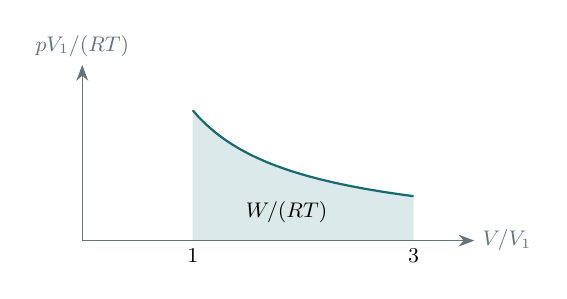
\begin{tikzpicture}[scale=.85,transform shape]
\begin{scope}[x=1.65cm,y=2.05cm]
\fill[accent!15,domain=1:3,samples=83](1,0)--plot(\x,{1/(\x-.2)-.3/\x^2})--(3,0)--cycle;
\draw[axis](0,0)--(3.55,0)node[right]{$V/V_1$};
\draw[axis](0,0)--(0,1.28)node[above]{$pV_1/(RT)$};
\draw[traj,domain=1:3,samples=85]plot(\x,{1/(\x-.2)-.3/\x^2});
\node[below]at(1,0){$1$};\node[below]at(3,0){$3$};
\node at(1.85,.21){$W/(RT)$};
\end{scope}
\end{tikzpicture}
\figcaption{变图热4.1V2\quad 可逆等温膨胀的对外功由压强曲线下的面积给出}
\end{minipage}\end{center}
\item 令 $V_2\to\infty$。在稳定单相的终态支上，由 $T_2=T_1+(a/C_V)(1/V_2-1/V_1)$ 得 $T_2\to T_\infty=T_1-a/(C_VV_1)$。取 $T_\infty>0$，温度对数趋于有限的 $C_V\ln(T_\infty/T_1)$，有效体积对数则按 $R\ln(V_2/V_1)$ 增长。变图热4.1V3画温度如何逼近下方水平线。若计算途中到了相共存区，改以相平衡求该段的温度和熵。
\begin{center}\begin{minipage}{.98\linewidth}\centering
\begin{tikzpicture}[scale=.85,transform shape]
\begin{scope}[x=.55cm,y=8cm]
\draw[axis](0,.73)--(10.35,.73)node[right]{$V_2/V_1$};
\draw[axis](0,.73)--(0,1.08)node[above]{$T_2/T_1$};
\draw[traj,domain=1:10,samples=99]plot(\x,{.8+.2/\x});
\draw[guide](0,.8)--(9.9,.8);
\node[left]at(0,.8){$.8$};\node[left]at(0,1){$1$};
\node[below]at(1,.73){$1$};
\node[below]at(10,.73){$10$};
\node[above]at(5.5,.91){$\varepsilon=.2$};
\end{scope}
\end{tikzpicture}
\figcaption{变图热4.1V3\quad 取吸引参数所对应的 $\varepsilon=0.2$，极限温度为 $0.8T_1$}
\end{minipage}\end{center}
\item 由 $\dd U=C_V\dd T+(a/V^2)\dd V$ 代入 $T\dd S=\dd U+p\dd V$。其中 $a/V^2$ 与状态方程中的 $-a/V^2$ 相消，留下 $R\dd V/(V-b)$。比较相同的两个温度与体积端点时，熵差表达式中因而没有 $a$。自由膨胀的温度终点仍随 $a$ 变，变图热4.1V4以 $V_2/V_1=3$ 给出 $T_2/T_1=1-(2/3)\varepsilon$。固定其余参数时，
\[
\frac{\partial \Delta S}{\partial a}=\frac{1/V_2-1/V_1}{T_2}<0,
\]
所以同一单相范围内增大吸引参数会减少熵增。
\begin{center}\begin{minipage}{.98\linewidth}\centering
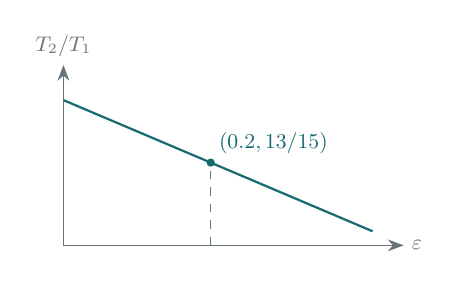
\begin{tikzpicture}[scale=.85,transform shape]
\begin{scope}[x=11cm,y=7cm]
\draw[axis](0,.69)--(.462,.69)node[right]{$\varepsilon$};
\draw[axis](0,.69)--(0,1.075)node[above]{$T_2/T_1$};
\draw[traj](0,1)--(.42,.72);
\fill[accent](.2,.8666667)circle(1.75pt)node[above right]{$(0.2,13/15)$};
\draw[guide](.2,.69)--(.2,.8666667);
\end{scope}
\end{tikzpicture}
\figcaption{变图热4.1V4\quad 在相同体积比下，吸引参数通过终温改变温度熵项}
\end{minipage}\end{center}
\item 取 $n$ 摩尔，$V$ 表示总容积。将摩尔容积换为 $V/n$，得 $p=nRT/(V-nb)-an^2/V^2$ 与 $U=U_*+nC_VT-an^2/V$。内能守恒给 $T_2-T_1=(an/C_V)(1/V_2-1/V_1)$，熵差为
\[
\Delta S=nC_V\ln(T_2/T_1)+nR\ln[(V_2-nb)/(V_1-nb)].
\]
变图热4.1V5在每摩尔初末容积相同的情况下比较1和2摩尔。总容积与有效容积都随 $n$ 放大，温度和摩尔熵差保持，故总熵差加倍。
\begin{center}\begin{minipage}{.98\linewidth}\centering
\begin{tikzpicture}[scale=.85,transform shape]
\node[left]at(0,1.8){$1\,\mathrm{mol}$};
\node[left]at(0,.4){$2\,\mathrm{mol}$};
\fill[accent!22](0,1.59)rectangle(1.12,2.01);
\draw[object](0,1.59)rectangle(2.24,2.01);
\fill[accent!22](0,.19)rectangle(2.24,.61);
\draw[object](0,.19)rectangle(4.48,.61);
\draw[guide](1.12,1.59)--(1.12,2.01);
\draw[guide](2.24,.19)--(2.24,.61);
\node[above]at(1.12,2.03){$v_1$};\node[above]at(2.24,2.03){$v_2$};
\node[below]at(2.24,.16){$2v_1$};\node[below]at(4.48,.16){$2v_2$};
\node[right]at(4.5,.65){每摩尔容积相同};
\end{tikzpicture}
\figcaption{变图热4.1V5\quad 相同每摩尔端态下，总容积与总熵差随物质的量成正比}
\end{minipage}\end{center}
\item 从初态作微小自由膨胀 $\delta V>0$。沿内能相等的平衡态曲线，$\delta T=-a\,\delta V/(C_VV_1^2)+O(\delta V^2)$。变图热4.1V6在初点用切线近似曲线。由 $T_1\delta S=\delta U+p_1\delta V+O(\delta V^2)$ 得 $\delta S=p_1\delta V/T_1+O(\delta V^2)$。若初态压强为正，膨胀的一阶熵差为正。实际绝热膨胀的熵产生等于完整端态熵差。
\begin{center}\begin{minipage}{.98\linewidth}\centering
\begin{tikzpicture}[scale=.85,transform shape]
\begin{scope}[x=7cm,y=7cm]
\draw[axis](.93,.83)--(1.58,.83)node[right]{$V/V_1$};
\draw[axis](.93,.83)--(.93,1.085)node[above]{$T/T_1$};
\draw[traj,domain=1:1.49,samples=71]plot(\x,{.8+.2/\x});
\draw[object,dashed](1,1)--(1.45,.91)node[below]{初点切线};
\fill[accent](1,1)circle(1.75pt);
\draw[guide](1,.905)--(1,1);
\draw[guide](1.2,.905)--(1.2,.967);
\draw[<->](1,.88)--(1.2,.88)node[midway,below]{$\delta V/V_1$};
\end{scope}
\end{tikzpicture}
\figcaption{变图热4.1V6\quad 微小体积增量的温度变化由初态等内能切线给出}
\end{minipage}\end{center}
\item 对同一对端点，可先在 $T_1$ 从 $V_1$ 等温走到 $V_2$，再在 $V_2$ 冷至 $T_2$。变图热4.1V7画出这条路径和先定容后等温的路径。两次等温步骤的熵变虽在不同温度下完成，均为 $R\ln[(V_2-b)/(V_1-b)]$。定容变温的熵变也都为 $C_V\ln(T_2/T_1)$。总熵差相同，各段热量则按各自的温度积分。路径取稳定单相区，经过共存区时另用相平衡或重选路径。
\begin{center}\begin{minipage}{.98\linewidth}\centering
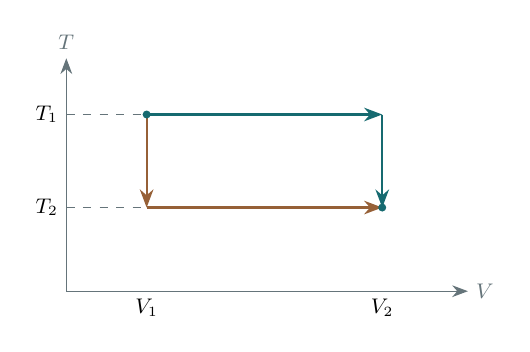
\begin{tikzpicture}[scale=.85,transform shape]
\draw[axis](0,0)--(6,0)node[right]{$V$};
\draw[axis](0,0)--(0,3.48)node[above]{$T$};
\draw[motion](1.2,2.64)--(4.72,2.64);
\draw[motion](4.72,2.64)--(4.72,1.25);
\draw[force](1.2,2.64)--(1.2,1.25);
\draw[force](1.2,1.25)--(4.72,1.25);
\fill[accent](1.2,2.64)circle(1.7pt);
\fill[accent](4.72,1.25)circle(1.7pt);
\draw[guide](0,2.64)--(1.2,2.64);\draw[guide](0,1.25)--(1.2,1.25);
\node[left]at(0,2.64){$T_1$};\node[left]at(0,1.25){$T_2$};
\node[below]at(1.2,0){$V_1$};\node[below]at(4.72,0){$V_2$};
\end{tikzpicture}
\figcaption{变图热4.1V7\quad 交换等温、定容两个步骤，保持初终态}
\end{minipage}\end{center}
\item 可逆绝热膨胀满足 $C_V\dd T/T=-R\dd V/(V-b)$，积分得 $T(V-b)^{R/C_V}=\mathrm{const}$。比较同一初态的两条曲线，
\[
\left(\frac{\dd T}{\dd V}\right)_S-
\left(\frac{\dd T}{\dd V}\right)_U=-\frac{p}{C_V}.
\]
在同一正压初态，可逆绝热线的斜率更负。变图热4.1V8取 $C_V/R=3/2,b/V_1=0.2,\varepsilon=0.2$。沿图中的等内能支，$\dd S=p\dd V/T>0$；沿可逆绝热线，熵保持初值。同一体积下 $(\partial S/\partial T)_V=C_V/T>0$，所以在图示的稳定单相区，实线在虚线上方。有限膨胀的终温分别由各自曲线积分求得。
\begin{center}\begin{minipage}{.98\linewidth}\centering
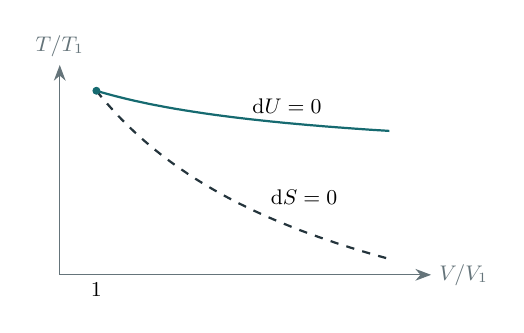
\begin{tikzpicture}[scale=.85,transform shape]
\begin{scope}[x=3.65cm,y=5.5cm]
\draw[axis](.85,.5)--(2.37,.5)node[right]{$V/V_1$};
\draw[axis](.85,.5)--(.85,1.07)node[above]{$T/T_1$};
\draw[traj,domain=1:2.2,samples=87]plot(\x,{.8+.2/\x});
\draw[object,dashed,domain=1:2.2,samples=87]plot(\x,{pow(.8/(\x-.2),2/3)});
\fill[accent](1,1)circle(1.7pt);
\node[above]at(1.78,.916){$\dd U=0$};
\node[above]at(1.85,.669){$\dd S=0$};
\node[below]at(1,.5){$1$};
\end{scope}
\end{tikzpicture}
\figcaption{变图热4.1V8\quad 在图示稳定单相区，同一终体积下等熵终温较低}
\end{minipage}\end{center}
\end{enumerate}

\clearpage

\pdfbookmark[2]{第 2 题 范德瓦耳斯氧气节流过程温度变化}{q2}

\section*{第 2 题\quad 范德瓦耳斯氧气节流过程温度变化}

1 mol氧气经绝热多孔塞节流，摩尔体积由高压侧$V_1=4.0\times10^{-3}\,\mathrm{m^3/mol}$增至低压侧$V_2=1.2\times10^{-2}\,\mathrm{m^3/mol}$。范德瓦耳斯参数$a=0.138\,\mathrm{Pa\cdot m^6/mol^2}$、$b=3.2\times10^{-5}\,\mathrm{m^3/mol}$，$C_V=20.8\,\mathrm{J/(mol\cdot K)}$恒定。流动动能和位能变化忽略。求温度变化：先写保留$b$、以初温$T_1$表示的关系，再在可忽略排斥体积对温差影响的近似下计算数值，并判断该近似需要什么条件。

\begin{center}\begin{minipage}{0.96\linewidth}\centering\begin{tikzpicture}[x=1cm,y=1cm,font=\small,every node/.append style={align=center}]\draw[object] (0,0) rectangle (7,1.8);\fill[pattern=north east lines] (3,0) rectangle (3.45,1.8);
\node at (1.4,1.2){高压侧\\$p_1,T_1,V_1$};\node at (5.4,1.2){低压侧\\$p_2,T_2,V_2$};
\draw[motion] (.4,.45)--(2.6,.45);\draw[motion] (3.8,.45)--(6.5,.45);\node[below] at (3.2,-.15){绝热多孔塞};\end{tikzpicture}\figcaption{图 热4.2　气体持续通过多孔塞，两侧流动带有压力功。}\end{minipage}\end{center}

\Needspace{5\baselineskip}

\pdfbookmark[3]{题型定位}{q2-h0}

\subsection*{题型定位}

用稳态绝热控制体的流动能量守恒求节流温差。保留排斥体积时读出温差对初温的依赖，再计算忽略该项的低密度估计。

\Needspace{5\baselineskip}

\pdfbookmark[3]{知识点}{q2-h1}

\subsection*{知识点}

稳态流动中，入口和出口的压力功分别与内能组成摩尔焓。范德瓦耳斯焓中，内能与 $pV$ 各含一项 $-a/V$。低密度展开后，温差中的吸引、排斥贡献分别由 $2a$ 和 $RbT_1$ 控制。


\Needspace{5\baselineskip}

\pdfbookmark[3]{物理图像}{q2-h2}

\subsection*{物理图像}

解图热4.2A的入口箭头表示上游推入一摩尔气体，出口箭头表示气体推开下游。解图热4.2B的直线每一点给一对不同的稳定端态。直线在 $T_*$ 过零，左边冷却、右边升温。

\Needspace{5\baselineskip}

\pdfbookmark[3]{解题入口}{q2-h3}

\subsection*{解题入口}

按解图热4.2A写 $U_1+p_1V_1=U_2+p_2V_2$。由状态方程求 $pV$，与 $U$ 相加得到 $H=U_*+A_iT-2a/V_i$。先解含 $T_1$ 的通式，再比较 $RbT_1/(2a)$，求可以略去排斥影响时的温差。


\Needspace{5\baselineskip}

\pdfbookmark[3]{标准解法}{q2-h4}

\subsection*{标准解法}

图中的气体流入、流出时，两侧压力分别推动入口气体和克服出口压力。对稳态绝热控制体，忽略动能、位能及轴功，每摩尔能量守恒为
\[
U_1+p_1V_1=U_2+p_2V_2,\qquad H_1=H_2.
\]
进、出口的流动功与相应的摩尔内能组成焓，因此两个端态等焓。
\begin{center}\begin{minipage}{0.96\linewidth}\centering\begin{tikzpicture}[x=1cm,y=1cm,font=\small,every node/.append style={align=center}]\draw[object] (0,0) rectangle (6,2);\fill[pattern=north east lines] (2.85,0) rectangle (3.15,2);
\draw[force] (-1,1)--(.5,1) node[above]{$p_1V_1$};\draw[force] (5.5,1)--(7,1) node[above]{$p_2V_2$};
\node at (1.45,1.1){$U_1$};\node at (4.5,1.1){$U_2$};\node[below] at (3,-.1){1 mol流入、1 mol流出：$U_1+p_1V_1=U_2+p_2V_2$};\end{tikzpicture}\figcaption{解图 热4.2A　进出口以各自的内能和流动功合计能量。}\end{minipage}\end{center}
解图热4.2A中入口、出口的压力功与内能一起构成焓，故两端焓相等。由$\dd U=C_V\dd T+a\dd V/V^2$积分得$U=U_*+C_VT-a/V$。再用状态方程计算
\[
pV=\frac{RTV}{V-b}-\frac aV,
\qquad H=U_*+\left(C_V+\frac{RV}{V-b}\right)T-\frac{2a}{V}.
\]
记$A_i=C_V+RV_i/(V_i-b)$，焓相等给
\[
A_2T_2-A_1T_1=2a\left(\frac1{V_2}-\frac1{V_1}\right),
\]
即保留排斥体积的结果为
\[
\result{\Delta T=T_2-T_1=\frac{(A_1-A_2)T_1+2a(1/V_2-1/V_1)}{A_2}}.
\]
其中
\[
A_1-A_2=Rb\left(\frac1{V_1-b}-\frac1{V_2-b}\right)>0.
\]
吸引作用给负温差，排斥体积项给与 $T_1$ 成正比的正贡献。保留 $b$ 时用上式表示温差随初温的变化。

\textbf{低密度近似。} 因$b/V_1=0.0080$、$b/V_2=0.00267$，可展开$V/(V-b)=1+b/V+O(b^2/V^2)$。当温差也小，保留$1/V$的一阶修正得
\[
\Delta T\simeq\frac{2a-RbT_1}{C_V+R}\left(\frac1{V_2}-\frac1{V_1}\right).
\]
$b/V$ 衡量排斥修正相对总焓的大小。温差由小的焓差决定，此时应比较 $RbT_1$ 与 $2a$ 两个首阶修正。若进一步满足$RbT_1\ll2a$，或明确采用忽略$b$对温差影响的模型，则
\begin{align*}
\Delta T&\simeq\frac{2a}{C_V+R}\left(\frac1{V_2}-\frac1{V_1}\right)\\
&=\frac{0.276}{20.8+8.31446}\left(\frac1{0.012}-\frac1{0.004}\right)\,\mathrm K
=-1.580\,\mathrm K\simeq-1.6\,\mathrm K.
\end{align*}
\begin{center}\begin{minipage}{0.96\linewidth}\centering\begin{tikzpicture}[x=3.4cm,y=1.1cm,font=\small]
\draw[axis] (0,0)--(1.7,0) node[right] {$u=T_1/(1000\,\mathrm K)$};
\draw[axis] (0,-1.5)--(0,1) node[above] {$\Delta T/\mathrm K$};
\draw[traj,domain=.2:1.4,samples=80] plot (\x,{1.538298224467*\x+(-1.578765403436)});
\draw[guide] (1.026306458868,0)--(1.026306458868,-1.4) node[below] {$T_*\simeq1026\,\mathrm K$};

\node[left] at (0,-1) {$-1$};\node[left] at (0,.5) {$0.5$};
\node[above] at (.5,0) {$0.5$};\node[above] at (1.5,0) {$1.5$};
\node at (.4,.55) {冷却};\node at (1.4,.75) {升温};
\end{tikzpicture}\figcaption{解图 热4.2B　给定两体积下的完整等焓温差，零点为有限过程分界$T_*$。}\end{minipage}\end{center}
\textbf{节流的升降温分界。} 一阶模型的冷却、升温分界约为$T_1=2a/(Rb)=1.037\times10^3\,\mathrm K$；解图热4.2B画的是保留b的完整关系，其零点与此首阶估计接近。若另给$T_1=300\,\mathrm K$，保留排斥参数$b$时算得$\Delta T=-1.117\,\mathrm K$。略去排斥项对温差的贡献才得到$-1.6\,\mathrm K$；保留该项时，温差随初温而变。取$a=b=0$，有$H=(C_V+R)T+U_*$，理想气体节流不变温。
\subsubsection*{控制体压力功和内能的两次吸引项}
解图热4.2A中，入口外侧气体把一摩尔气体推入控制体，
对它作压力功$p_1V_1$；出口的一摩尔气体则对出口外侧作功$p_2V_2$。
若通过同样一摩尔的稳态时间段，控制体不积累能量，
流入的内能与入口功之和等于流出的内能与出口功之和。
这里U、H取摩尔内能和摩尔焓，V取摩尔体积，
因此热容量、参数及压力功的单位也按每摩尔配套。
侧壁绝热，能量随进出口的气体与压力功穿过控制面。
入口、出口的压力功使本题守恒焓；刚性封闭容器向真空膨胀时则守恒内能。

由状态方程的热力学恒等式，
\[
\left(\frac{\partial U}{\partial V}\right)_T
=T\frac R{V-b}-\left(\frac{RT}{V-b}-\frac a{V^2}\right)
=\frac a{V^2}.
\]
积分内能时$\int aV^{-2}\dd V=-a/V$，
状态方程的$pV$中又含$-a/V$，
内能和流动功各贡献一次，得到焓的吸引项 $-2a/V$。
取 $b=0$ 比较从 $V_1$ 到 $V_2$ 的两种过程。节流把焓中的吸引项变化 $-2a(1/V_2-1/V_1)$ 用热容量 $C_V+R$ 换成温变；封闭气体向真空膨胀时，$\Delta U=0$，温差为 $a(1/V_2-1/V_1)/C_V$。这两个温降的比值（节流比自由膨胀）为 $2C_V/(C_V+R)$。

\subsubsection*{保留排斥项后的精确分界}
完整等焓式对初温$T_1$是仿射关系，斜率$(A_1-A_2)/A_2>0$。
令温差为零，可得本次给定两个体积的分界温度
\[
\begin{aligned}
T_*&=\frac{2a(1/V_1-1/V_2)}{A_1-A_2}\\
&=\frac{2a}{Rb}
\left(1-\frac b{V_1}\right)
\left(1-\frac b{V_2}\right).
\end{aligned}
\]
因此完整温差也可写成
\[
\Delta T=\frac{A_1-A_2}{A_2}(T_1-T_*).
\]
低于$T_*$冷却、高于它升温，但仍须位于相应稳定单相支并保证真实流动从高压到低压。
本题$T_*\simeq1.026\times10^3$ K，
与低密度首阶的$2a/(Rb)\simeq1.037\times10^3$ K接近而不完全相同。
解图热4.2B的零点给这两个指定体积的等温端态。若要了解相邻端态如何随压强变化，则沿等焓条件求温压导数。

忽略b时的数值分子为
$2a(1/V_2-1/V_1)=0.276(83.3333-250)=-46.0$ J/mol，
分母$C_V+R=29.11446$ J/(mol\,K)，故温差为$-1.580$ K。
两个大体积相对b都很大，只保证状态方程中排斥修正小；
温差由焓的相近量相减得到，保留的一阶修正却可能与吸引项同量级。
首阶忽略排斥贡献的相对判据是$RbT_1/(2a)\ll1$，
在300 K时这一比值约0.289，排斥项使温差绝对值减少约0.46 K。
完整式的$-1.117$ K与$-1.580$ K正体现这种差别。

稳态气体仍处于同一稳定气相时，每摩尔熵差为
\[
\Delta S=C_V\ln\frac{T_2}{T_1}
+R\ln\frac{V_2-b}{V_1-b}.
\]
若补给初温300 K，使用完整终温，得熵增约$9.10$ J/(mol\,K)，为正。
节流时外壁绝热，给定流向上的熵差等于每摩尔流过多孔塞所产生的熵。
若所需的是微分焦耳—汤姆孙系数，则应从$\dd H=0$对相邻状态求导，
在各相邻状态求温压导数的零点，可得到微分反转曲线。


\Needspace{5\baselineskip}

\pdfbookmark[3]{关键洞察}{q2-h5}

\subsection*{关键洞察}

本题是在几项大能量之间求小的焓差。即使 $b/V_1=0.008$，在300 K时排斥项和吸引项比值也已约0.289。有限的两端体积给 $T_*$，相邻端态另由微分的等焓斜率处理。

\Needspace{5\baselineskip}

\pdfbookmark[3]{易错点}{q2-h6}

\subsection*{易错点}

进、出口的压力功用各自的压强和摩尔体积。以摩尔量配套 $R,C_V,a,b$。保留排斥项时，初温进入结果。判断流向时沿给定两端分别算压强。等焓的压降产生熵，正熵差由端态熵函数计算。

\Needspace{5\baselineskip}

\pdfbookmark[3]{课堂讲解建议}{q2-h7}

\subsection*{课堂讲解建议}

先照解图热4.2A分别画压力功箭头，问哪一方对入口、出口处的一摩尔气体做功。由 $U$ 与 $pV$ 的两个修正得到系数 $2a$，再将各项归入 $A_iT$ 和 $-2a/V_i$。

在解图热4.2B读直线过零点，依次讨论300 K和高于 $T_*$ 的端态。用变图热4.2V5把300 K的温差拆为吸引项和排斥项，说明小的 $b/V_i$ 为何仍使数值变化约0.46 K。然后让学生算一组端压与熵差，判断方向并说明不可逆压降的能量流动。

\Needspace{5\baselineskip}

\pdfbookmark[3]{变式训练}{q2-h8}

\subsection*{变式训练}

\begin{enumerate}
\item 取 $a=b=0$，摩尔焓为 $H=U_*+(C_V+R)T$。变图热4.2V1中，两个节流端点具有同一个焓值，该水平线在焓温直线上只对应一个温度，故 $T_2=T_1$。若改成可逆绝热膨胀，气体由 $\dd U=-p\dd V$ 把内能转为外功，在同一理想气体模型内会降温。
\begin{center}\begin{minipage}{.98\linewidth}\centering
\begin{tikzpicture}[scale=.85,transform shape]
\draw[axis](0,0)--(5.55,0)node[right]{$T$};
\draw[axis](0,0)--(0,3.12)node[above]{$H$};
\draw[traj](0,.55)--(4.8,2.85)node[above right]{$U_*+(C_V+R)T$};
\draw[guide](0,1.9875)--(3,1.9875)--(3,0);
\fill[accent](3,1.9875)circle(1.8pt);
\node[left]at(0,1.9875){$H_1=H_2$};\node[below]at(3,0){$T_1=T_2$};
\end{tikzpicture}
\figcaption{变图热4.2V1\quad 理想气体的等焓端点在焓温图中重合}
\end{minipage}\end{center}
\item 把进、出口体积交换，并重新取入口温度为300 K。忽略 $b$，体积倒数差变号，所以等焓温差变成 $+1.580\,\mathrm K$。用同一状态方程计算这组代数端态，$V=0.012$ 处为约207 kPa，$V=0.004$ 处为约618 kPa。变图热4.2V2表明该方向是低压到高压。自然流过无轴功多孔塞的气体从高压侧向低压侧流，这组反向端态只给出了等焓方程的代数解。
\begin{center}\begin{minipage}{.98\linewidth}\centering
\begin{tikzpicture}[scale=.85,transform shape]
\draw[axis](0,0)--(5.45,0)node[right]{两端};
\draw[axis](0,0)--(0,3.6)node[above]{$p/\mathrm{kPa}$};
\fill[accent!25](.8,0)rectangle(1.53,1.035);
\fill[warm!35](3.47,0)rectangle(4.2,3.09);
\node[above]at(1.165,1.035){$207$};\node[above]at(3.835,3.09){$618$};
\node[below]at(1.165,0){设为入口};\node[below]at(3.835,0){设为出口};
\draw[motion,dashed](1.58,1.5)--(3.22,1.5)node[midway,above]{交换方向};
\end{tikzpicture}
\figcaption{变图热4.2V2\quad 交换容积后的等焓候选端态，出口压强高于入口}
\end{minipage}\end{center}
\item 用温差反求吸引参数。忽略 $b$ 时，变图热4.2V3的直线斜率为 $2(1/V_2-1/V_1)/(C_V+R)$，故 $a=(C_V+R)\Delta T/[2(1/V_2-1/V_1)]$。扩容使体积倒数差为负，实测冷却也给 $\Delta T<0$，所以两负量相除得正 $a$。保留 $b$ 并已知 $T_1$ 时，改用
\[
a=\frac{A_2\Delta T-(A_1-A_2)T_1}{2(1/V_2-1/V_1)}.
\]
\begin{center}\begin{minipage}{.98\linewidth}\centering
\begin{tikzpicture}[scale=.85,transform shape]
\draw[axis](0,0)--(5.8,0)node[right]{$a/(\mathrm{Pa\,m^6/mol^2})$};
\draw[axis](0,-3.05)--(0,.6)node[above]{$\Delta T/\mathrm K$};
\draw[traj](0,0)--(5.05,-2.891);
\draw[guide](2.76,0)--(2.76,-1.58)--(0,-1.58);
\fill[accent](2.76,-1.58)circle(1.7pt);
\node[above]at(2.76,0){$0.138$};
\node[left]at(0,-1.58){$-1.58$};
\end{tikzpicture}
\figcaption{变图热4.2V3\quad 忽略排斥修正时，温差随吸引参数线性下降}
\end{minipage}\end{center}
\item 有限过程的升降温分界为 $T_*=[2a/(Rb)](1-b/V_1)(1-b/V_2)\simeq1026\,\mathrm K$。变图热4.2V4比较完整直线与低密度首阶直线，后者由 $2a-RbT_1=0$ 给约 $1037\,\mathrm K$。完整模型中，稳定气体从高压侧流到低压侧，$T_1<T_*$ 时冷却，$T_1>T_*$ 时升温。这一零点随两指定体积变化。
\begin{center}\begin{minipage}{.98\linewidth}\centering
\begin{tikzpicture}[scale=.85,transform shape]
\begin{scope}[x=.033cm,y=11cm]
\draw[axis](950,0)--(1115,0)node[right]{$T_1/\mathrm K$};
\draw[axis](950,-.135)--(950,.155)node[above]{$\Delta T/\mathrm K$};
\draw[traj,domain=960:1100,samples=45]plot(\x,{.001538298*(\x-1026.3065)});
\draw[object,dashed,domain=960:1100,samples=45]plot(\x,{0.001523084634*(\x-1037.3493889)});
\fill[accent](1026.3065,0)circle(1.5pt);
\fill[ink](1037.35,0)circle(1.5pt);
\node[above left]at(1026.3065,0){$1026$};
\node[below right]at(1037.35,0){$1037$};
\node[above]at(1070,.09){完整式};
\node[below]at(987,-.09){首阶式};
\end{scope}
\end{tikzpicture}
\figcaption{变图热4.2V4\quad 放大零温差附近，区分完整有限过程与首阶分界}
\end{minipage}\end{center}
\item 给定 $T_1=300\,\mathrm K$。完整式中吸引项为 $-1.5788\,\mathrm K$，排斥项为 $+0.4615\,\mathrm K$。变图热4.2V5从零向左画吸引项，再向右加排斥项，终点 $\Delta T=-1.1173\,\mathrm K$，所以 $T_2\simeq298.883\,\mathrm K$。取 $b=0$ 得 $-1.5800\,\mathrm K$，温降绝对值比完整值约大41\%。这些数值使用题给的常摩尔热容量。
\begin{center}\begin{minipage}{.98\linewidth}\centering
\begin{tikzpicture}[scale=.85,transform shape]
\draw[axis](-5.47,0)--(.8,0)node[right]{$\Delta T/\mathrm K$};
\draw[motion](0,1.52)--(-4.7364,1.52)node[midway,above]{吸引 $-1.579$};
\draw[force](-4.7364,.74)--(-3.3519,.74)node[midway,above]{排斥 $+0.461$};
\draw[guide](0,0)--(0,1.52);
\draw[guide](-4.7364,.74)--(-4.7364,1.52);
\draw[guide](-3.3519,0)--(-3.3519,.74);
\fill[accent](-3.3519,0)circle(1.75pt)node[below]{$-1.117$};
\node[below]at(0,0){$0$};
\end{tikzpicture}
\figcaption{变图热4.2V5\quad 300 K 时，排斥项抵消了一部分吸引降温}
\end{minipage}\end{center}
\item 改为封闭容器向真空自由膨胀。摩尔内能守恒给 $\Delta T_U=a(1/V_2-1/V_1)/C_V\simeq-1.106\,\mathrm K$。同一对体积下，取 $b=0$ 的节流温差为 $\Delta T_H\simeq-1.580\,\mathrm K$。变图热4.2V6用降温量比较，二者之比为 $2C_V/(C_V+R)\simeq1.429$。吸引项系数从 $a$ 变为 $2a$，对应分母也从 $C_V$ 变成 $C_V+R$。
\begin{center}\begin{minipage}{.98\linewidth}\centering
\begin{tikzpicture}[scale=.85,transform shape]
\draw[axis](0,0)--(5.6,0)node[right]{过程};
\draw[axis](0,0)--(0,3.25)node[above]{$-\Delta T/\mathrm K$};
\fill[accent!28](.82,0)rectangle(1.73,1.991);
\fill[accent!55](3,0)rectangle(3.91,2.844);
\node[above]at(1.275,1.991){$1.106$};\node[above]at(3.455,2.844){$1.580$};
\node[below]at(1.275,0){等内能};\node[below]at(3.455,0){等焓，$b=0$};
\end{tikzpicture}
\figcaption{变图热4.2V6\quad 相同体积变化下，两个守恒条件给出不同的温降}
\end{minipage}\end{center}
\item 保留宏观动能和位能，记摩尔质量为 $\mu$。变图热4.2V7的进出口能量流各含三项，稳态绝热、无轴功时
\[
H_1+\frac{\mu u_1^2}{2}+\mu g z_1
=H_2+\frac{\mu u_2^2}{2}+\mu g z_2.
\]
同高度且出口较快时，减少的摩尔焓转为宏观动能。若壁面传热 $Q$ 或气体对轴做功 $W_s$，则在上式的入口总量上加 $Q-W_s$，两量均按一摩尔计算。
\begin{center}\begin{minipage}{.98\linewidth}\centering
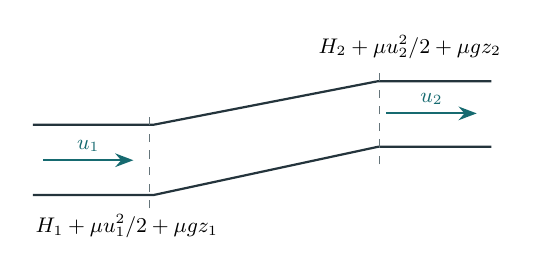
\begin{tikzpicture}[scale=.85,transform shape]
\draw[object](-.6,1.5)--(1.2,1.5)--(4.55,2.15)--(6.25,2.15);
\draw[object](-.6,.45)--(1.2,.45)--(4.55,1.17)--(6.25,1.17);
\draw[motion](-.45,.97)--(.9,.97)node[midway,above]{$u_1$};
\draw[motion](4.68,1.67)--(6.03,1.67)node[midway,above]{$u_2$};
\draw[guide](1.14,.25)--(1.14,1.68);
\draw[guide](4.58,.91)--(4.58,2.32);
\node[below]at(.8,.28){$H_1+\mu u_1^2/2+\mu gz_1$};
\node[above]at(5.03,2.36){$H_2+\mu u_2^2/2+\mu gz_2$};
\end{tikzpicture}
\figcaption{变图热4.2V7\quad 进出口同时带走或带入焓、动能和位能}
\end{minipage}\end{center}
\item 给定入口300 K并使用完整终温298.883 K。将熵差拆成 $C_V\ln(T_2/T_1)\simeq-0.0776\,\mathrm{J/(mol\cdot K)}$ 与 $R\ln[(V_2-b)/(V_1-b)]\simeq9.1789\,\mathrm{J/(mol\cdot K)}$。变图热4.2V8比较两项的符号，合计 $\Delta S\simeq9.1013\,\mathrm{J/(mol\cdot K)}$。稳态绝热时外壁熵流为零，这一正值是每摩尔流过产生的熵。
\begin{center}\begin{minipage}{.98\linewidth}\centering
\begin{tikzpicture}[scale=.85,transform shape]
\draw[axis](0,0)--(5.72,0)node[right]{熵差项};
\draw[axis](0,-.62)--(0,3.34)node[above]{$\mathrm{J/(mol\cdot K)}$};
\fill[accent!40](.64,0)rectangle(1.45,2.7537);
\fill[warm!45](2.46,0)rectangle(3.27,-.0233);
\fill[accent!61](4.12,0)rectangle(4.93,2.7304);
\node[above]at(1.045,2.7537){$9.1789$};
\node[below]at(2.865,-.03){$-0.0776$};
\node[above]at(4.525,2.7304){$9.1013$};
\node[below]at(1.045,0){容积};
\node[above]at(2.865,0){温度};
\node[below]at(4.525,0){合计};
\end{tikzpicture}
\figcaption{变图热4.2V8\quad 有效容积增长带来的正熵差主要决定总熵增}
\end{minipage}\end{center}
\end{enumerate}

\clearpage

\pdfbookmark[2]{第 3 题 乙醚临界现象中气液质量比}{q3}

\section*{第 3 题\quad 乙醚临界现象中气液质量比}

纯乙醚封装在玻璃管内，管容积恰等于所装乙醚的总临界体积。加热时气、液两相共存，达到临界点时界面消失。其摩尔状态方程为$(p+a/V^2)(V-b)=RT$。已知摩尔临界体积$V_K$；温度$T$时，饱和气相与液相的摩尔体积分别为$V_g,V_l$。求两相各占总体积的比例$B_g,B_l$及两相质量比例。在$V_g\gg V_l$时，用$a,b,T$近似表示$V_l$。若20℃封装，取$T_K=466.95\,\mathrm K$、$p_K=34.60\,\mathrm{atm}$，求所需液相体积比例，并核查近似的精度。

\begin{center}\begin{minipage}{0.96\linewidth}\centering\begin{tikzpicture}[x=1cm,y=1cm,font=\small,every node/.append style={align=center}]\draw[object] (0,0) rectangle (1.7,3.4);\fill[blue!20] (0,0) rectangle (1.7,1.05);
\draw[object] (0,1.05)--(1.7,1.05);\node at (.85,.5){液相};\node at (.85,2.2){气相};
\node[right] at (2,2.9){总量$\nu$\\管容积$\nu V_K$};\draw[motion] (3,.5)--(3,1.7) node[above]{缓慢加热};\end{tikzpicture}\figcaption{图 热4.3　两相共存时摩尔数分配与体积分配不同。}\end{minipage}\end{center}

\Needspace{5\baselineskip}

\pdfbookmark[3]{题型定位}{q3-h0}

\subsection*{题型定位}

由临界装填的总物质的量和总容积求气液分配，再用范德瓦耳斯方程确定液、气两个共存端点。比较近似与完整结果对装填比例的影响。

\Needspace{5\baselineskip}

\pdfbookmark[3]{知识点}{q3-h1}

\subsection*{知识点}

定总体积给杠杆规则。纯物质两相摩尔质量相同，质量分数等于摩尔分数，体积分数由各相摩尔数乘对应摩尔体积求得。在等温线上以 $\dd g=V\dd p$ 积分，摩尔吉布斯势相等给等面积条件。临界处两个体积导数同时为零。


\Needspace{5\baselineskip}

\pdfbookmark[3]{物理图像}{q3-h2}

\subsection*{物理图像}

图热4.3固定管容积为 $\nu V_K$。解图热4.3A的共存水平线连接液相小体积端点和气相大体积端点。线段内改变的是两相分配。解图热4.3B的杠杆上，气相分数由靠近液相端的短臂给出，气相摩尔体积较大，乘上去后仍可占管容积过半。

\Needspace{5\baselineskip}

\pdfbookmark[3]{解题入口}{q3-h3}

\subsection*{解题入口}

先解总摩尔数和总容积的两个守恒式。确定 $x_g,x_l$ 后分别乘 $V_g/V_K,V_l/V_K$ 得体积分数。用同压与等面积共同求 $V_l,V_g$。在气相摩尔体积远大的情形，保留 $b$ 求液相小根，并用等温负斜率选稳定支。


\Needspace{5\baselineskip}

\pdfbookmark[3]{标准解法}{q3-h4}

\subsection*{标准解法}

设总量为$\nu$ mol，玻璃管容积为$\nu V_K$。温度$T<T_K$时，气、液摩尔数分别$n_g,n_l$，同一种乙醚的两相摩尔质量相同。守恒约束为
\[
n_g+n_l=\nu,\qquad n_gV_g+n_lV_l=\nu V_K.
\]
相减消元给摩尔分数及质量分数
\[
x_g=\frac{n_g}{\nu}=\frac{V_K-V_l}{V_g-V_l},\qquad
x_l=\frac{n_l}{\nu}=\frac{V_g-V_K}{V_g-V_l},
\qquad \frac{m_g}{m_l}=\frac{V_K-V_l}{V_g-V_K}.
\]
体积比例还要乘各自摩尔体积，故
\[
\result{B_g=\frac{(V_K-V_l)V_g}{(V_g-V_l)V_K},\quad
B_l=\frac{(V_g-V_K)V_l}{(V_g-V_l)V_K}}.
\]
二者和为1；要写百分数时再乘$100\%$。可共存的装填条件为$V_l\le V_K\le V_g$。这些比例与总量$\nu$无关。
\begin{center}\begin{minipage}{0.96\linewidth}\centering\begin{tikzpicture}[x=1.85cm,y=2.8cm,font=\small]
\draw[axis] (.3,0)--(3.65,0) node[right] {$v=V/V_K$};
\draw[axis] (.3,0)--(.3,1.03) node[above] {$p/p_K$};
\fill[blue!15] plot[domain=0.553360458439:1.145305205726,samples=90] (\x,{6.8/(3*\x-1)-3/(\x*\x)})--(1.145305205726,0.504491649791)--(0.553360458439,0.504491649791)--cycle;
\fill[warm!18] plot[domain=1.145305205726:3.127639292398,samples=90] (\x,{6.8/(3*\x-1)-3/(\x*\x)})--(3.127639292398,0.504491649791)--(1.145305205726,0.504491649791)--cycle;

\draw[traj,domain=.525:3.5,samples=190] plot (\x,{6.8/(3*\x-1)-3/(\x*\x)});
\draw[object] (0.553360458439,0.504491649791)--(3.127639292398,0.504491649791);
\draw[guide] (0.553360458439,0) node[below left] {$V_l/V_K$}--(0.553360458439,0.504491649791);
\draw[guide] (3.127639292398,0) node[below] {$V_g/V_K$}--(3.127639292398,0.504491649791);
\node[above right] at (3.15,.55) {$p_s/p_K$};

\draw[guide] (1,0) node[below] {$1$}--(1,.4);
\node at (2,.9) {$T/T_K=0.85$};
\node at (2,.75) {上下阴影面积相等};
\end{tikzpicture}\figcaption{解图 热4.3A　按状态方程绘制的共存线与等面积，两端分别为液相与气相。}\end{minipage}\end{center}
\textbf{求共存摩尔体积。} 解图热4.3A的水平线为饱和压强$p_s$，两端点满足相同温度和压强。等面积条件为
\[
\int_{V_l}^{V_g}p(V,T)\dd V=p_s(V_g-V_l).
\]
代入并逐项积分，得
\[
RT\ln\frac{V_g-b}{V_l-b}-a\left(\frac1{V_l}-\frac1{V_g}\right)
=p_s(V_g-V_l),
\]
另外两个端点条件为
\[
p_s=\frac{RT}{V_l-b}-\frac a{V_l^2}
=\frac{RT}{V_g-b}-\frac a{V_g^2}.
\]
消去$p_s$可写成完整组
\begin{align*}
RT\ln\frac{V_g-b}{V_l-b}
&=a\left(\frac1{V_l}-\frac1{V_g}\right)
\left(\frac{V_g-b}{V_g}+\frac{V_l-b}{V_l}\right),\\
RT\left(\frac1{V_l-b}-\frac1{V_g-b}\right)
&=a\left(\frac1{V_l^2}-\frac1{V_g^2}\right).
\end{align*}
\textbf{气相体积远大于液相时。} 若$V_g\gg V_l$，忽略上述方程中的$1/V_g$小项，第二式简化为$RT/(V_l-b)=a/V_l^2$，即
\[
RTV_l^2-aV_l+ab=0,\qquad
V_l=\frac{a\pm\sqrt{a(a-4bRT)}}{2RT}.
\]
应取液相的高密度稳定根，即负号。除$b<V_l<V_K=3b$之外，还须满足$\left(\partial p/\partial V\right)_T<0$；由近似根满足$RT=a(V_l-b)/V_l^2$，有
\[
\left(\frac{\partial p}{\partial V}\right)_{T,V_l}
=-\frac{RT}{(V_l-b)^2}+\frac{2a}{V_l^3}
=\frac{a(V_l-2b)}{V_l^3(V_l-b)}.
\]
分母为正，负斜率要求$V_l<2b$，因此取较小的根。较大根位于 $V>2b$ 处，等温斜率为正。第一式则给
\[
RT\ln\frac{V_g-b}{V_l-b}\simeq\frac a{V_l}\left(2-\frac b{V_l}\right)
=RT+\frac a{V_l},
\quad V_g\simeq(V_l-b)\exp\left(1+\frac a{RTV_l}\right)+b.
\]
\begin{center}\begin{minipage}{0.96\linewidth}\centering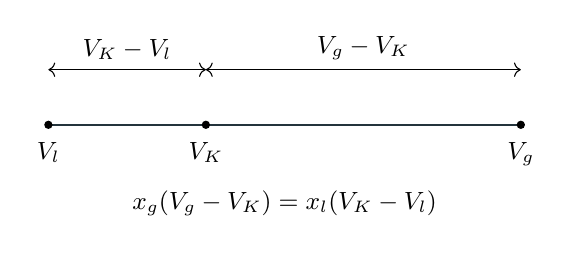
\begin{tikzpicture}[x=1cm,y=1cm,font=\small,every node/.append style={align=center}]\draw[object] (0,1)--(6,1);\foreach \x/\lab in {0/V_l,2/V_K,6/V_g}{\fill (\x,1) circle (1.5pt);\node[below] at (\x,.9){$\lab$};}
\draw[<->] (0,1.7)--(2,1.7) node[midway,above]{$V_K-V_l$};\draw[<->] (2,1.7)--(6,1.7) node[midway,above]{$V_g-V_K$};
\node at (3,0){$x_g(V_g-V_K)=x_l(V_K-V_l)$};\end{tikzpicture}\figcaption{解图 热4.3B　杠杆规则给摩尔分数，乘各相摩尔体积才得体积分数。}\end{minipage}\end{center}
\textbf{20℃装填数值。} 解图热4.3B用两相摩尔体积分配总物质的量，下面再由临界条件确定计算所需的气体常量。临界等温线在临界点有水平拐点，因此
\[
-\frac{RT_K}{(V_K-b)^2}+\frac{2a}{V_K^3}=0,\qquad
\frac{2RT_K}{(V_K-b)^3}-\frac{6a}{V_K^4}=0.
\]
分别改写为$RT_K=2a(V_K-b)^2/V_K^3$与
$RT_K=3a(V_K-b)^3/V_K^4$，相除得$2V_K=3(V_K-b)$。
故$V_K=3b$，回代第一式求$T_K$，再代状态方程求$p_K$，得到
\[
V_K=3b,\qquad p_K=\frac a{27b^2},\qquad T_K=\frac{8a}{27Rb}.
\]
因此，用SI单位$p_K=34.60\times101325\,\mathrm{Pa}$，有
\[
b=\frac{RT_K}{8p_K}=1.38427\times10^{-4}\,\mathrm{m^3/mol},\qquad
a=27p_Kb^2=1.81385\,\mathrm{Pa\cdot m^6/mol^2},
\]
\[
V_K=4.15282\times10^{-4}\,\mathrm{m^3/mol},\qquad T=293.15\,\mathrm K.
\]
按$V_g\gg V_l$近似，
\[
V_l=1.83846\times10^{-4},\qquad V_g=7.20938\times10^{-3}\quad(\mathrm{m^3/mol}),
\]
\[
B_l=\frac{(V_g-V_K)V_l}{(V_g-V_l)V_K}=0.428117,\quad
\result{B_l\simeq42.8\%,\quad B_g\simeq57.2\%\quad\text{（近似）}}.
\]
同一温度下，联立等压与等面积条件数值求解得
\[
V_l=1.83202\times10^{-4},\quad V_g=5.51626\times10^{-3}\,\mathrm{m^3/mol},
\quad p_s=3.93619\times10^5\,\mathrm{Pa},
\]
\[
\result{B_l=42.20\%,\quad B_g=57.80\%\quad\text{（完整范德瓦耳斯模型）}}.
\]
近似液相体积与完整值接近，最终液相体积比例相差约0.62个百分点。气相体积由指数式给出，对指数误差较敏感。接近临界点时 $V_g/V_l$ 趋于1，改用完整共存方程。近似要求比较 $V_g$ 与 $V_l$，而固定的 $V_K=3b$ 和液相摩尔体积 $V_l>b$ 属同一量级。
\subsubsection*{等面积条件与两相平衡的联系}
解图热4.3A的两个共存端点温度、压强和摩尔吉布斯势分别相等。
等温时$\dd g=V\dd p$，把状态方程的均匀流体支作数学延拓，分部积分得
\[
g_g-g_l=\int_{V_l}^{V_g}V\frac{\partial p}{\partial V}\dd V
=p_s(V_g-V_l)-\int_{V_l}^{V_g}p\dd V.
\]
所以两相化学势相等恰给等面积条件。
图中水平线上各点是两相按不同比例混合的状态。回环由均匀流体状态方程延拓得到，其中正斜率段的等温压缩系数为负，属于不稳定的均匀状态。
图A选$T/T_K=0.85$绘制完整状态方程，低于水平线和高于水平线的阴影面积相等。
这张图说明共存条件；20℃的具体端点仍由其自身温度求解。

还可展开上述消元的中间计算。
两端等压式相减并约去$V_g-V_l$，得
\[
RT=\frac{a(V_g+V_l)(V_g-b)(V_l-b)}{V_g^2V_l^2},\qquad
p_s=\frac{a[V_gV_l-b(V_g+V_l)]}{V_g^2V_l^2}.
\]
将第二式乘$V_g-V_l$，
\[
p_s(V_g-V_l)=a\left(\frac1{V_l}-\frac1{V_g}\right)
\left(1-\frac b{V_l}-\frac b{V_g}\right).
\]
与等面积积分式中的吸引项相加，正好得到前面完整方程组的第一个式子。
用两端同压确定同一等温线上的候选端点，再用等面积条件选出饱和压强。

\subsubsection*{液相小根的适用温度与体积误差}
为了避免低温下$a-\sqrt{a(a-4bRT)}$的相近量相减，
液相近似根也可有理化为
\[
V_l=\frac{2ab}{a+\sqrt{a(a-4bRT)}}.
\]
温度趋低时它趋近b，并仍应从大于b的一侧取值。
这个二次方程有实根的条件为
\[
T\le\frac{a}{4Rb}=\frac{27}{32}T_K.
\]
等号处二根合为 $V_l=2b$，等温斜率为零。因而近似式给出严格稳定液相根的必要条件是 $T<27T_K/32$，还要满足 $V_g\gg V_l$。解图热4.3A取 $0.85T_K$，已超过这个近似上限，图中的端点由完整两相平衡方程求出。

20℃完整解给气相摩尔分数约0.04352、液相约0.95648，
气液质量比约0.04550，而气相体积比例却约57.80\%。
解图热4.3B的较短臂$V_K-V_l$决定较少的气相物质的量，
乘上大得多的气相摩尔体积后，它仍能占过半管容积。
用给出的完整数值逐项比较，液相体积近似误差约0.35\%，
气相体积约30.7\%，液相体积比例则相差约0.62个百分点。
三个数分别以液相摩尔体积、气相摩尔体积和液相体积分数为比较对象。完整求解保留了范德瓦耳斯模型中的气相倒数体积项。要进一步比较实际乙醚的相平衡，还需使用实验数据或更精细的状态方程。


\Needspace{5\baselineskip}

\pdfbookmark[3]{关键洞察}{q3-h5}

\subsection*{关键洞察}

严格稳定的液相近似根要求 $T<27T_K/32$ 且 $V_g\gg V_l$，接近临界点时用完整共存条件。气相体积由指数式确定，液相体积仅约0.35\%的近似差足以影响气相体积。20℃完整模型的气相质量分数约4.35\%，体积分数约57.80\%。

\Needspace{5\baselineskip}

\pdfbookmark[3]{易错点}{q3-h6}

\subsection*{易错点}

$V_K$ 是整个管子的平均摩尔体积，总容积为 $\nu V_K$。等压端点还以等面积条件确定。液相二次小根选 $b<V_l<2b$，对应正等温压缩系数。临界附近改求完整共存曲线。把 $p_K$ 由 atm 转为 Pa 之后再与 SI 制的 $R$ 联用。

\Needspace{5\baselineskip}

\pdfbookmark[3]{课堂讲解建议}{q3-h7}

\subsection*{课堂讲解建议}

在图热4.3上分别标气、液各自的物质的量与实际体积。用解图热4.3B的短臂、长臂写出摩尔数比，请学生说明气体为何质量少而体积大。

在解图热4.3A移动一条水平线，让学生用 $\dd g=V\dd p$ 解释只有等面积时两端化学势相等。再用变图热4.3V6看两条近似根的切线方向，得到压缩时压力上升的稳定液相分支。

把20℃的两组端点并列，用变图热4.3V7分别读气相摩尔体积和液相占比的差值。最后沿变图热4.3V4接近临界点，讨论等临界平均容积时的杠杆分式怎样取极限。

\Needspace{5\baselineskip}

\pdfbookmark[3]{变式训练}{q3-h8}

\subsection*{变式训练}

\begin{enumerate}
\item 把平均摩尔体积设为 $\bar V$，由 $x_gV_g+(1-x_g)V_l=\bar V$ 得 $x_g=(\bar V-V_l)/(V_g-V_l)$。在 $V_l\le\bar V\le V_g$ 时，两相分配非负。变图热4.3V1画临界附近的两条共存支和一条偏左的定容线。升温时液相端点先向右碰到这条定容线，该点 $x_g=0$，继续沿定容线升温便进入单相。取 $\bar V>V_K$ 的定容线时，先从气相一侧离开共存区。
\begin{center}\begin{minipage}{.98\linewidth}\centering
\begin{tikzpicture}[scale=.85,transform shape]
\draw[axis](0,0)--(6.05,0)node[right]{$V/V_K$};
\draw[axis](0,0)--(0,3.15)node[above]{$T/T_K$};
\draw[traj,domain=.62:5.26,samples=93]plot(\x,{2.56-.31*(\x-3)^2});
\draw[object,dashed](2.1,0)--(2.1,2.8);
\draw[guide](3,0)--(3,2.56);
\fill[accent](2.1,2.3089)circle(1.8pt)node[above left]{$x_g=0$};
\fill[accent](3,2.56)circle(1.75pt)node[above right]{临界点};
\node[below]at(2.1,0){$\bar V/V_K$};\node[below]at(3,0){$1$};
\node[above]at(4.39,1.55){共存气相};
\node[left]at(.88,1.07){共存液相};
\end{tikzpicture}
\figcaption{变图热4.3V1\quad 靠近临界点的共存曲线示意，较小等容线先穿过液相端点}
\end{minipage}\end{center}
\item 在同一温度的共存线上，$n_g/n_l=(\bar V-V_l)/(V_g-\bar V)$，乘同一个摩尔质量得同样的质量比。气体与液体所占容积之比还乘 $V_g/V_l$。以本题20℃完整解为例，变图热4.3V2的上行气相给约 $4.35\%$ 的质量，下行给约 $57.80\%$ 的容积。这两行的总长度各归一到1。
\begin{center}\begin{minipage}{.98\linewidth}\centering
\begin{tikzpicture}[scale=.85,transform shape]
\foreach \y/\cut/\lab in {1.72/.261/质量,.28/3.468/容积}{
\fill[accent!38](0,\y)rectangle(\cut,{\y+.5});
\fill[rulegray](\cut,\y)rectangle(6,{\y+.5});
\draw[object](0,\y)rectangle(6,{\y+.5});
\node[left]at(0,{\y+.24}){\lab};}
\draw[guide](.261,2.22)--(.74,2.61);
\node[right]at(.74,2.61){气相 $4.35\%$};
\node at(1.72,.52){气相 $57.80\%$};
\node at(4.73,.52){液相};
\end{tikzpicture}
\figcaption{变图热4.3V2\quad 两相摩尔质量相同，气液占据的空间由各自摩尔体积决定}
\end{minipage}\end{center}
\item 给定气液质量比 $q$，纯物质有 $n_g=qn_l$ 和 $n_g+n_l=\nu$，因此 $\bar V=(qV_g+V_l)/(q+1)$，总管容积为 $\nu\bar V$。变图热4.3V3以 $x_g=q/(1+q)$ 为横坐标，线段相应位置的纵值就是所需的 $\bar V$。例如 $q=1$ 时气、液摩尔数相等，取两端体积的算术平均。两端体积取自同一个等温共存态。
\begin{center}\begin{minipage}{.98\linewidth}\centering
\begin{tikzpicture}[scale=.85,transform shape]
\draw[axis](0,0)--(5.77,0)node[right]{$x_g=q/(1+q)$};
\draw[axis](0,0)--(0,3.25)node[above]{$\bar V$};
\draw[traj](0,.55)--(4.95,2.9);
\fill[accent](2.475,1.725)circle(1.75pt)node[above left]{$q=1$};
\draw[guide](2.475,0)--(2.475,1.725);
\draw[guide](4.95,0)--(4.95,2.9)--(0,2.9);
\node[left]at(0,.55){$V_l$};\node[left]at(0,2.9){$V_g$};
\node[below]at(2.475,0){$1/2$};\node[below]at(4.95,0){$1$};
\end{tikzpicture}
\figcaption{变图热4.3V3\quad 先依据气相质量比求气相摩尔分数，再读出装填体积}
\end{minipage}\end{center}
\item 令 $\tau=1-T/T_K>0$ 和 $z=V/V_K-1$。临界附近 $p/p_K=1-4\tau+6\tau z-\frac32z^3+O(\tau z^2,z^4)$。保留所列项时，等面积条件关于 $z=0$ 对称，水平线 $p/p_K=1-4\tau$ 交两端于 $z\simeq\pm2\sqrt\tau$。变图热4.3V4画出这两支的领先项。取固定 $\bar V=V_K$，两个杠杆臂在首阶等长，故 $x_g,x_l\to1/2$。两相密度相同的极限下，占据体积的比例也趋于 $1/2$，临界点之后界面消失。
\begin{center}\begin{minipage}{.98\linewidth}\centering
\begin{tikzpicture}[scale=.85,transform shape]
\draw[axis](0,0)--(6.18,0)node[right]{$\tau$};
\draw[axis](0,-1.42)--(0,1.62)node[above]{$V/V_K-1$};
\draw[traj,domain=0:5.7,samples=96]plot(\x,{.52*sqrt(\x)});
\draw[object,dashed,domain=0:5.7,samples=96]plot(\x,{-.52*sqrt(\x)});
\draw[<->](4.62,0)--(4.62,1.1177);
\draw[<->](4.62,0)--(4.62,-1.1177);
\node[above]at(4.28,1.22){气相端};
\node[below]at(4.28,-1.23){液相端};
\node[below left]at(0,0){$0$};
\end{tikzpicture}
\figcaption{变图热4.3V4\quad 临界附近，两端点与临界体积的距离在首阶同时按 $\sqrt{\tau}$ 缩小}
\end{minipage}\end{center}
\item 任取共存端点间的 $\bar V$，有 $x_g+x_l=1$ 及 $x_gV_g+x_lV_l=\bar V$。因此 $B_l=x_lV_l/\bar V$、$B_g=x_gV_g/\bar V$，均在0至1之间且和为1。变图热4.3V5取归一化的共存体积例 $V_l=V_*,V_g=4V_*$，画出两体积分数在端点间变化。先由同温同压、等化学势求端点，再套这两条分配式。
\begin{center}\begin{minipage}{.98\linewidth}\centering
\begin{tikzpicture}[scale=.85,transform shape]
\draw[axis](0,0)--(6.08,0)node[right]{$\bar V/V_*$};
\draw[axis](0,0)--(0,2.97)node[above]{体积分数};
\draw[traj,domain=1.35:5.4,samples=77]plot(\x,{2.32*(4-\x/1.35)/(3*\x/1.35)});
\draw[object,dashed,domain=1.35:5.4,samples=77]plot(\x,{2.32*4*(\x/1.35-1)/(3*\x/1.35)});
\draw[guide](0,2.32)--(5.4,2.32);
\node[left]at(0,2.32){$1$};\node[below]at(1.35,0){$1$};\node[below]at(5.4,0){$4$};
\node[above]at(4.32,2.12){$B_g$};\node[above]at(2.66,.9){$B_l$};
\end{tikzpicture}
\figcaption{变图热4.3V5\quad 液相和气相的体积分数在整个共存线上的和为1}
\end{minipage}\end{center}
\item 在液相近似方程 $RT/(V_l-b)=a/V_l^2$ 上，
$p'(V_l)=a(V_l-2b)/[V_l^3(V_l-b)]$。因此正等温压缩系数对应 $b<V_l<2b$ 的负斜率小根。变图热4.3V6取 $T=0.65T_K$，用 $z=V/b$ 作横坐标，两个近似零压根约为1.352和3.840，斜率一负一正。实根存在要求 $T\le27T_K/32$。等号处两根合在 $V_l=2b$，斜率为零；有严格负斜率的小根要求 $T<27T_K/32$。气、液摩尔体积接近时，转用完整的共存等温线。
\begin{center}\begin{minipage}{.98\linewidth}\centering
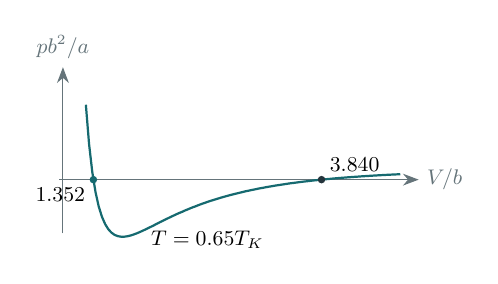
\begin{tikzpicture}[scale=.85,transform shape]
\begin{scope}[x=1.37cm,y=12cm]
\draw[axis](.98,0)--(4.9,0)node[right]{$V/b$};
\draw[axis](1.02,-.067)--(1.02,.14)node[above]{$pb^2/a$};
\draw[traj,domain=1.27:4.7,samples=99]plot(\x,{(8*.65/27)/(\x-1)-1/\x^2});
\fill[accent](1.352085,0)circle(1.6pt);
\fill[ink](3.840223,0)circle(1.6pt);
\node[below left]at(1.352085,0){$1.352$};
\node[above right]at(3.840223,0){$3.840$};
\node[below right]at(1.89,-.054){$T=0.65T_K$};
\end{scope}
\end{tikzpicture}
\figcaption{变图热4.3V6\quad 低压近似的较小根位于等温负斜率的液相支}
\end{minipage}\end{center}
\item 给定20℃，将等压、等面积条件同时求根得 $V_l=1.83202\times10^{-4}$、$V_g=5.51626\times10^{-3}\,\mathrm{m^3/mol}$。代入杠杆式得 $B_l\simeq42.20\%$。变图热4.3V7把各个量相对完整模型的近似偏差归一比较。液相体积约高 $0.35\%$，气相约高 $30.7\%$。液相占比约由 $42.20\%$ 变为 $42.81\%$，绝对差约 $0.62$ 个百分点，体积分数的相对差约 $1.46\%$。结论适用于给定状态方程。
\begin{center}\begin{minipage}{.98\linewidth}\centering
\begin{tikzpicture}[scale=.85,transform shape]
\draw[axis](0,0)--(6.03,0)node[right]{各量};
\draw[axis](0,0)--(0,3.46)node[above]{相对偏差};
\foreach \x/\h/\lab/\val in {1.1/.035/{液相摩尔\\体积}/{0.35},3.05/3.07/{气相摩尔\\体积}/{30.7},5/.146/{液相体积\\分数}/{1.46}}{
\fill[accent!38]({\x-.38},0)rectangle({\x+.38},\h);
\node[above]at(\x,\h){$\val\%$};
\node[below,align=center]at(\x,0){\lab};}
\end{tikzpicture}
\figcaption{变图热4.3V7\quad 液相摩尔体积的近似偏差小，气相体积的偏差较大}
\end{minipage}\end{center}
\item 把小根分子有理化，得
\[
V_l=\frac{2ab}{a+\sqrt{a(a-4bRT)}}.
\]
当 $RTb/a\to0$，分母趋于 $2a$，故 $V_l/b$ 由上侧趋于1。令 $\chi=RTb/a$，还可展开 $V_l/b=1+\chi+2\chi^2+O(\chi^3)$。变图热4.3V8把有理化形式与一阶展开画在一起。有理化使分母为加法，便于低温数值计算；两式均从忽略气相倒数体积项的模型出发。
\begin{center}\begin{minipage}{.98\linewidth}\centering
\begin{tikzpicture}[scale=.85,transform shape]
\begin{scope}[x=19cm,y=4cm]
\draw[axis](0,.94)--(.28,.94)node[right]{$\chi$};
\draw[axis](0,.94)--(0,2.13)node[above]{$V_l/b$};
\draw[traj,domain=0:.25,samples=105]plot(\x,{2/(1+sqrt(max(0,1-4*\x)))});
\draw[object,dashed,domain=0:.25,samples=73]plot(\x,{1+\x});
\fill[accent](0,1)circle(1.7pt);
\node[left]at(0,1){$1$};
\node[below]at(.25,.94){$1/4$};
\node[above left]at(.218,1.50){有理化小根};
\node[below]at(.157,1.148){$1+\chi$};
\end{scope}
\end{tikzpicture}
\figcaption{变图热4.3V8\quad 从低温向临界近似上限升温，小根从 $b$ 向 $2b$ 增大}
\end{minipage}\end{center}
\end{enumerate}

\clearpage

\pdfbookmark[2]{第 4 题 毛细现象永动机方案的热力学破绽}{q4}

\section*{第 4 题\quad 毛细现象永动机方案的热力学破绽}

图示密闭装置与温度恒定的大气导热。A为完全润湿的毛细区域，B为实心隔挡，其外侧空间C较大；导管D内有可无摩擦移动的活塞E。活门F在一定正压差下打开、压差近零时关闭；G的开闭顺序相反。所有空白空间只含该液体蒸汽，底部及毛细区装同一液体。设计者假定毛细凹液面附近的饱和蒸汽压$p_1$与下方平液面附近的$p_2$相同，又用蒸汽的重力压差，声称能循环地从单一热源取热并全部变为活塞功。先说明这一推证的过程，再否定它并导出$p_1,p_2$的定量关系。设毛细半径$r$，升高$h$，液体与蒸汽密度为$\rho_l,\rho_v$，表面张力系数为$\sigma$；采用密度近似恒定的小高度模型。

\begin{center}\begin{minipage}{.96\linewidth}\centering
\begin{tikzpicture}[x=.85cm,y=.85cm,font=\small]
\draw[object] (0,0) rectangle (8,6);
\fill[blue!12] (0,0) rectangle (8,1.2);
\fill[blue!12] (0,1.2)--(1.8,1.2)--(1.8,3.2) .. controls (1.2,2.94) and (.6,2.94) .. (0,3.2)--cycle;
\fill[pattern=north east lines] (1.8,1.2) rectangle (4.8,3.2);
\draw[object] (1.8,1.2) rectangle (4.8,3.2);
\node[fill=white,inner sep=2pt] at (3.3,2.1){B：实心隔挡};\node at (.85,1.9){A};
\draw[traj] (0,3.2) .. controls (.6,2.94) and (1.2,2.94) .. (1.8,3.2);
\draw[object] (1.8,4)--(1.8,6) (1.8,4)--(3.6,4) (4.2,4)--(4.8,4);
\draw[object,very thick] (4.8,3.2)--(4.8,4);
\draw[object] (4.8,3.6)--(8.7,3.6);
\draw[object] (1.8,4)--(2.15,3.57);\node[left] at (1.75,3.75){F};
\draw[object] (4.2,4)--(3.85,3.62);\node[above] at (3.9,4.08){G};
\node at (2.95,3.6){D};\node[above right] at (4.8,4.03){E};
\node at (5.7,5.0){C：蒸汽空间};
\fill (.7,3.3) circle (1.3pt) node[above]{$p_1$};
\fill (5.8,3.3) circle (1.3pt) node[above]{$p_0$};
\fill (5.8,1.3) circle (1.3pt) node[above]{$p_2$};
\draw[guide] (5.4,3.2)--(7.5,3.2) (5.4,1.2)--(7.5,1.2);
\draw[<->] (7.2,1.2)--(7.2,3.2) node[midway,right]{$h$};
\draw[object] (0,0) rectangle (8,6);
\end{tikzpicture}\figcaption{图 热4.4　F连通A与活塞左腔D，G连通D与C；活塞右侧属于C。阀片位置仅示意通路。}\end{minipage}\end{center}

\Needspace{5\baselineskip}

\pdfbookmark[3]{题型定位}{q4-h0}

\subsection*{题型定位}

用静力和曲率修正分析毛细装置。先跟踪设计者的设想，再从两侧实际压强找出推出阶段的力和功。

\Needspace{5\baselineskip}

\pdfbookmark[3]{知识点}{q4-h1}

\subsection*{知识点}

液体与蒸汽分别满足 $\dd p=-\rho g\dd z$。同高度的连通蒸汽在等温平衡时等压，凹液面满足 $p_v-p_l=2\sigma/r$。两相摩尔吉布斯势相等可得同一个小曲率压差。单热源下，若装置循环复原而输出净功，总熵会减少。


\Needspace{5\baselineskip}

\pdfbookmark[3]{物理图像}{q4-h2}

\subsection*{物理图像}

图热4.4中F接A与D，G接D与C，活塞右侧一直在C中。解图热4.4B、C分别画设想的推出和返回。解图热4.4A中 $p_1,p_0$ 处于同一高度，$p_2$ 取下方平液面处的值。向上时液相压强降得较快，跨凹液面的压强增量补足两种梯度的差。

\Needspace{5\baselineskip}

\pdfbookmark[3]{解题入口}{q4-h3}

\subsection*{解题入口}

先按F、G的两种开闭复述假想循环。以平液面为零点写液相压力、汽相压力和凹面压差，配合同高度的 $p_1=p_0$ 求高度与 $p_1-p_2$。再把两相化学势在平液面饱和压强附近展开，解释曲率为何改变饱和蒸汽压。


\Needspace{5\baselineskip}

\pdfbookmark[3]{标准解法}{q4-h4}

\subsection*{标准解法}

先按图热4.4的通路追踪设计者假设的循环：F连接A与D，G连接D与C，活塞E右面始终受到C的蒸汽压力。若$p_1=p_2$，而C中蒸汽下部压强$p_2=p_0+\rho_vgh$，便有$p_1>p_0$。于是F打开、G关闭，D中蒸汽把E向右推，输出功约为$\int(p_1-p_0)\dd V>0$。压差消失后F关闭、G打开，解图热4.4C中D经G与C相通，设计者认为等压下E可无功返回，C内部分蒸汽凝结、毛细区部分液体蒸发，使装置完全复原。循环内能变化为零，输出功便来自同一温度的大气所供热量。
\begin{center}\begin{minipage}{.97\linewidth}\centering
\begin{tikzpicture}[x=.72cm,y=.72cm,font=\small]
\foreach \dx in {0,7.4}{\begin{scope}[shift={(\dx,0)}]
\draw[object] (0,0) rectangle (5.7,2.3);
\draw[object] (1.4,0)--(1.4,.65) (1.4,1.45)--(1.4,2.3);
\draw[object] (1.4,1.45)--(2.65,1.45) (3.3,1.45)--(3.7,1.45);
\draw[object,very thick] (3.7,.65)--(3.7,1.45);\draw[object] (3.7,1.05)--(5.9,1.05);
\draw[object] (1.4,.65)--(3.7,.65);
\node at (.6,1.05){A};\node at (2.45,1.03){D};\node at (4.75,1.85){C};
\node[below] at (1.4,-.1){F};\node[above] at (3.5,1.65){G};\node[below] at (3.8,.45){E};
\end{scope}}
\draw[motion] (.9,1.05)--(2.05,1.05);\draw[very thick,warm] (2.65,1.45)--(3.3,1.45);
\draw[motion] (3.9,-.55)--(5.2,-.55) node[midway,below]{推出};
\node[above,align=center] at (2.8,2.5){F开、G闭\\假设$p_1>p_0$};
\draw[very thick,warm] (8.8,.65)--(8.8,1.45);
\draw[<->,accent,thick] (10.35,1.05)--(10.35,2.0);
\draw[motion] (12.5,-.55)--(11.2,-.55) node[midway,below]{设想等压返回};
\node[above,align=center] at (10.2,2.5){F闭、G开\\D、C等压};
\end{tikzpicture}\figcaption{解图 热4.4B、C　设计者设想的做功与复位阶段；左图所需的平衡压差实际不存在。}\end{minipage}\end{center}

解图热4.4B、C所设想的做功及复位若能循环，这相当于只从一个热源取热、把它全部转为功而不留下其他变化，违反第二定律。下面用静力和表面张力求两侧压强，说明即使活塞无摩擦，推出阶段也缺少压差。
\begin{center}\begin{minipage}{0.96\linewidth}\centering\begin{tikzpicture}[x=1cm,y=1cm,font=\small,every node/.append style={align=center}]\draw[object] (0,0)--(6,0);\node[below] at (4.7,-.1){平液面：$p_2$};
\draw[object] (.5,0)--(.5,2.4);\draw[object] (1.1,0)--(1.1,2.4);\draw[traj] (.5,2.15) .. controls (.7,1.85) and (.9,1.85) .. (1.1,2.15);
\node[left] at (.5,2.2){$p_1$};\node[right] at (1.1,1.75){$p_A$};\fill (4.7,2) circle (1.5pt) node[right]{$p_0$};
\draw[guide] (1.2,2)--(5.2,2);\draw[<->] (3.1,0)--(3.1,2) node[midway,right]{$h$};
\node at (3,-.8){$p_1-p_A=2\sigma/r$；液体梯度$\rho_lg$，蒸汽梯度$\rho_vg$};\end{tikzpicture}\figcaption{解图 热4.4A　先在两种介质中分别比较高度，再跨越凹液面。}\end{minipage}\end{center}
\textbf{按图逐层比较压强。} 沿解图热4.4A的高度线比较，在下方平液面处，液体与蒸汽压强均取$p_2$。高度$h$处，毛细液面下方液体压强为$p_A$，其上方蒸汽为$p_1$；C内同高度蒸汽压强为$p_0$。静水关系分别给
\[
p_A=p_2-\rho_lgh,\qquad p_0=p_2-\rho_vgh.
\]
凹液面处蒸汽侧压强高于液体侧，完全润湿时曲率半径为$r$，单界面的拉普拉斯关系是
\[
p_1-p_A=\frac{2\sigma}{r}.
\]
同温且连通的蒸汽在同一高度平衡，应有$p_1=p_0$。四式联立：
\[
\frac{2\sigma}{r}=(\rho_l-\rho_v)gh,
\qquad h=\frac{2\sigma}{(\rho_l-\rho_v)gr}.
\]
因此毛细凹液面上方的饱和蒸汽压与下方平液面附近的值不同：
\[
\result{p_1-p_2=-\rho_vgh
=-\frac{2\sigma\rho_v}{(\rho_l-\rho_v)r}<0}.
\]
活塞两边在同一高度的正确平衡压强其实相同，假想循环的驱动压差不再存在。

\textbf{饱和压强为何还与曲率有关。} 固定温度时，饱和压强还随液面曲率改变。凹液面的液侧压强较低，液相化学势降低，平衡蒸汽压也随之降低。可用两相化学势相等计算这一修正。令同温平液面饱和压强为$p_f$，凹液面处蒸汽压为$p_v$、液压为$p_l$，
摩尔质量仍记为$\mu$，两相摩尔吉布斯势记为$g_v,g_l$。
等温时$\dd g=V_m\dd p$；理想蒸汽有$V_{m,v}=RT/p$，不可压液体有$V_{m,l}=\mu/\rho_l$，故
\[
g_v(T,p_v)-g_v(T,p_f)=RT\ln\frac{p_v}{p_f},\qquad
g_l(T,p_l)-g_l(T,p_f)=\frac{\mu}{\rho_l}(p_l-p_f).
\]
平液面和凹液面处各自满足两相吉布斯势相等，再用$p_l=p_v-2\sigma/r$消去液压：
\[
RT\ln\frac{p_v}{p_f}=\frac{\mu}{\rho_l}
\left(p_v-p_f-\frac{2\sigma}{r}\right).
\]
小曲率修正下，$p_v-p_f\simeq p_f\ln(p_v/p_f)$；右侧这一项相对左侧的系数为
$\mu p_f/(\rho_lRT)=\rho_v/\rho_l\ll1$，可以略去。于是
\[
\ln\frac{p_{\rm concave}}{p_{\rm flat}}
\simeq-\frac{2\sigma\mu}{\rho_lRTr}.
\]
蒸汽静力平衡同时给$p(h)=p(0)\exp[-\mu gh/(RT)]$。在 $\rho_v\ll\rho_l$ 且 $\mu gh/(RT)\ll1$ 时，指数关系的首项给 $-\rho_vgh$，与前面的常密度式一致。
\subsubsection*{闭合压强回路与装置复位}
沿解图热4.4A从下方平液面出发，
先在液体中上升h，再跨越凹液面，最后在蒸汽中下降h回到同一平液面，
回到同一平液面时压强恢复为起点值，所以三段压强改变量相加为零：
\[
-\rho_lgh+\frac{2\sigma}{r}+\rho_vgh=0.
\]
三项沿回路的符号依次为负、正、正。上升和下降两段的合计是 $-(\rho_l-\rho_v)gh$。
由同高度蒸汽平衡$p_1=p_0$及$p_2-p_0=\rho_vgh$，
得到$p_1<p_2$。图B的活塞两侧在同一高度，实际相连的蒸汽压强是$p_1$与$p_0$，二者相等。$p_2$位于更低处，$p_2-p_0$是蒸汽柱重量造成的压差。

在两侧等压时，蒸汽对活塞的合力为零，所设返回段没有蒸汽驱动力。若用重物、弹簧或外力带动复位，循环要计入它们的状态变化和复位功。即使活塞与阀门均无摩擦，正功段两侧的$p_1=p_0$也给零压差。
若假设整个装置真能循环且从唯一温度T的热源吸收Q并输出同量功，
系统熵恢复，热源熵减少Q/T，整体熵变化为$-Q/T<0$。
整体熵减少违反第二定律。如果液量、界面面积或重物高度在末态改变，这些量的变化也属于过程结果，装置尚未完成循环复原。

\subsubsection*{保留蒸汽密度的一阶曲率修正}
前面的化学势方程还可在小压差下保留蒸汽密度项。
令$\delta p=p_v-p_f$，在平液面饱和压强附近线性化，得
\[
\left(\frac{RT}{p_f}-\frac{\mu}{\rho_l}\right)\delta p
=-\frac{2\sigma\mu}{\rho_lr}.
\]
使用平液面蒸汽的理想关系$\rho_v=\mu p_f/(RT)$，整理为
\[
\delta p=-\frac{2\sigma\rho_v}{(\rho_l-\rho_v)r}.
\]
它与液、汽静力及拉普拉斯关系联立的答案一致。
再令$\rho_v/\rho_l\ll1$，才退化为前述常用的凹面Kelvin近似。
这说明忽略液体摩尔体积相对于蒸汽摩尔体积的贡献，与忽略上升高度式中的蒸汽密度，是相配套的近似。
接近临界点时，以同一温度下的两相密度、表面张力和真实蒸汽性质求平衡。

若完全润湿改成接触角$\theta$，圆管静态弯月面的曲率项变为$2\sigma\cos\theta/r$，
毛细高度和相应小压差也同时乘$\cos\theta$。
从液体内部量接触角。$\theta<\pi/2$ 时，凹液面高于平液面，液面上蒸汽压较低。$\theta>\pi/2$ 时，弯月面凸起而整体低于大液面，两处蒸汽压差反号。


\Needspace{5\baselineskip}

\pdfbookmark[3]{关键洞察}{q4-h5}

\subsection*{关键洞察}

$p_2-p_0$ 是低处到同高度的蒸汽压差，活塞两侧却比较同一高度的 $p_1$ 与 $p_0$。曲率导致 $p_1=p_0<p_2$，推出的压差为零。若另设复位装置，循环还要包括复位装置的状态变化与功。

\Needspace{5\baselineskip}

\pdfbookmark[3]{易错点}{q4-h6}

\subsection*{易错点}

将凹液面的高压侧放在蒸汽一边。拉普拉斯压差取单界面系数2。液面和活塞处的压强按各自高度使用；求首个非零汽压差时保留 $\rho_v$。线性静力式用于小高度，理想蒸汽在较大高度使用指数式。

\Needspace{5\baselineskip}

\pdfbookmark[3]{课堂讲解建议}{q4-h7}

\subsection*{课堂讲解建议}

请学生沿图热4.4画F、G的两条通路，在活塞两侧填同一高度的压强。再从解图热4.4A的平液面开始，沿液柱上升，跨过凹面，再沿蒸汽下降。用三个压差相加为零求毛细高度。

比较解图热4.4B与变图热4.4V1的活塞两侧数值。接着把等压复位改成外力复位，让学生说出循环末还要恢复哪些状态。

用变图热4.4V3画单热源、装置和负载间的能量箭头，写系统与环境的熵变。随后改变弯月面方向或接触角，让学生用变图热4.4V8同时读出高度和汽压差的符号。

\Needspace{5\baselineskip}

\pdfbookmark[3]{变式训练}{q4-h8}

\subsection*{变式训练}

\begin{enumerate}
\item 设想的第一阶段F开、G关，活塞左腔D接毛细区A。变图热4.4V1上行可读 $p_{\rm D}=p_1$，右腔C在同高度给 $p_0$，而平衡时 $p_1=p_0$。故第一阶段的蒸汽推力 $A_E(p_{\rm D}-p_0)=0$，其中 $A_E$ 为活塞面积。第二阶段F关、G开，D接C，同样是两侧等压。阀门耗散可消耗机械能，理想平衡下两阶段的蒸汽推力已经为零。
\begin{center}\begin{minipage}{.98\linewidth}\centering
\begin{tikzpicture}[scale=.85,transform shape]
\foreach \y/\leftlab/\rightlab/\stage in {1.75/A/{D,\ p_1}/{F开，G关},.22/C/{D,\ p_0}/{F关，G开}}{
\node[draw] (left) at(0,\y){$\leftlab$};
\node[draw] (right) at(2.9,\y){$\rightlab$};
\draw[motion](left.east)--(right.west)node[midway,above]{\stage};
\draw[object,very thick](4.02,{\y-.38})--(4.02,{\y+.38});
\node[right]at(4.27,\y){C，$p_0$};}
\node[above]at(4.03,2.28){活塞E};
\end{tikzpicture}
\figcaption{变图热4.4V1\quad 切换蒸汽通路后，活塞左腔仍与右腔等压}
\end{minipage}\end{center}
\item 把活塞和阀门取为理想元件。装置等温平衡时，变图热4.4V2的压差曲线沿零线，推程的净汽压功和返程的净汽压功都为零。若外力带动活塞返回，则以 $W_{\rm ext}=\int F_{\rm ext}\dd x$ 计入外力功，并在一周末恢复施力装置的状态。单热源条件下，合计一周的净正功仍受第二定律限制。
\begin{center}\begin{minipage}{.98\linewidth}\centering
\begin{tikzpicture}[scale=.85,transform shape]
\draw[axis](0,0)--(6,0)node[right]{过程};
\draw[axis](0,-.58)--(0,1.8)node[above]{$p_{\rm D}-p_0$};
\draw[traj,line width=1.2pt](.53,0)--(5.65,0);
\draw[guide](2.8,-.32)--(2.8,1.26);
\node[above]at(1.55,.41){推程};
\node[above]at(4.2,.41){返程};
\node[left]at(0,0){$0$};
\node[below]at(2.8,-.32){切换通路};
\end{tikzpicture}
\figcaption{变图热4.4V2\quad 理想静力过程中，两个阶段的活塞压差都在零线}
\end{minipage}\end{center}
\item 按变图热4.4V3给出一个假想能量流：唯一热源以温度 $T$ 放出 $Q$，装置把 $W$ 交给负载。周期首尾的内能相同，所以 $Q=W$。装置熵回复初值，负载只接收机械功，热源熵变为 $-Q/T$。由此总熵变为 $-Q/T$，因此循环复原时要求 $Q\le0$，即该流向下 $W\le0$。
\begin{center}\begin{minipage}{.98\linewidth}\centering
\begin{tikzpicture}[scale=.85,transform shape]
\node[draw,align=center] (S) at(0,1){单一热源\\$T$};
\node[draw,align=center] (D) at(3.1,1){装置\\$\Delta U=\Delta S=0$};
\node[draw] (L) at(6.28,1){负载};
\draw[motion](S.east)--(D.west)node[midway,above]{$Q$};
\draw[motion](D.east)--(L.west)node[midway,above]{$W$};
\node[below]at(0,.39){熵变 $-Q/T$};
\end{tikzpicture}
\figcaption{变图热4.4V3\quad 单热源向循环装置供热，负载接收机械功}
\end{minipage}\end{center}
\item 只用第二定律时，把装置、热源和所有会改变状态的物体一起纳入。变图热4.4V4左侧给装置复原和单热源放热时的两项熵变，若只有这两项，正功要求的 $Q>0$ 使总熵减少。若另有燃料、温差、液量或重物高度发生变化，右侧所示的各项也进入总能量与总熵。此时净功取决于这些量在全过程端点的实际变化。
\begin{center}\begin{minipage}{.98\linewidth}\centering
\begin{tikzpicture}[scale=.85,transform shape]
\draw[axis](0,0)--(5.78,0)node[right]{对象};
\draw[axis](0,-1.75)--(0,1.52)node[above]{熵变};
\fill[ink](.98,0)circle(1.65pt);
\draw[force](2.65,0)--(2.65,-1.1)node[below]{$-Q/T$};
\draw[guide](4.51,-1.05)--(4.51,1.05);
\node[right]at(4.56,.78){按其状态求};
\node[below]at(.98,0){装置};
\node[above]at(2.65,.06){热源};
\node[below]at(4.51,0){其他物体};
\end{tikzpicture}
\figcaption{变图热4.4V4\quad 判定一周是否成立，要把各对象的终态都计入}
\end{minipage}\end{center}
\item 令 $\epsilon=\rho_v/\rho_l$，并记 $h_0=2\sigma/(\rho_lgr)$。精确到本题常密度模型，有 $h/h_0=(1-\epsilon)^{-1}$，$p_1-p_2=-(2\sigma/r)\epsilon/(1-\epsilon)$。变图热4.4V5画出小 $\epsilon$ 下的压差首阶。求高度的零阶可用 $h_0$，而汽压差的首个非零项是 $-\rho_vgh_0$。令 $\rho_v=0$ 时，这一压差也为零。
\begin{center}\begin{minipage}{.98\linewidth}\centering
\begin{tikzpicture}[scale=.85,transform shape]
\draw[axis](0,0)--(5.55,0)node[right]{$\epsilon$};
\draw[axis](0,0)--(0,2.95)node[above]{$-(p_1-p_2)r/(2\sigma)$};
\draw[traj,domain=0:5,samples=80]plot(\x,{7.5*(\x/20)/(1-\x/20)});
\draw[object,dashed](0,0)--(5,1.875);
\node[above]at(4.48,2.18){常密度式};
\node[below]at(4.24,1.51){首阶项};
\node[below]at(5,0){$0.25$};
\end{tikzpicture}
\figcaption{变图热4.4V5\quad 蒸汽密度较小时，汽压差从一阶项开始}
\end{minipage}\end{center}
\item 改成半径 $r$ 的凸球液面，拉普拉斯式变为 $p_l-p_v=2\sigma/r$。平液面给基准 $p_f$。用相同的等温吉布斯势积分，低密度蒸汽和小曲率下得
\[
\ln(p_{\rm convex}/p_f)\simeq\frac{2\sigma\mu}{\rho_lRTr}.
\]
变图热4.4V6把凸滴与凹液面并列，两侧相对同一个平液面压强的修正方向相反。若蒸发和重建液滴，界面面积变化带来的能量也进入完整过程。
\begin{center}\begin{minipage}{.98\linewidth}\centering
\begin{tikzpicture}[scale=.85,transform shape]
\fill[accent!20](0,1.24)circle(.68);
\draw[traj](0,1.24)circle(.68);
\draw[force](0,1.24)--(.68,1.24)node[midway,above]{$r$};
\node[above]at(0,2.01){凸滴};
\node[below]at(0,.51){$p_v>p_f$};
\fill[accent!20](3.13,.31)--(4.63,.31)--(4.63,1.89)..controls(4.1,1)and(3.68,1)..(3.13,1.89)--cycle;
\draw[object](3.13,.31)--(3.13,2.11) (4.63,.31)--(4.63,2.11);
\draw[traj](3.13,1.89)..controls(3.68,1)and(4.1,1)..(4.63,1.89);
\node[above]at(3.88,2.11){凹液面};
\node[below]at(3.88,.23){$p_v<p_f$};
\end{tikzpicture}
\figcaption{变图热4.4V6\quad 凸滴和平液面相比汽压较高，凹液面则较低}
\end{minipage}\end{center}
\item 高度较大时，把蒸汽看成理想气体，$\dd p/\dd z=-\mu gp/(RT)$ 给 $p_1=p_2e^{-\kappa h}$，其中 $\kappa=\mu g/(RT)$。液体仍取不可压，故 $p_A=p_2-\rho_lgh$。再代入 $p_1-p_A=2\sigma/r$，得到
\[
\rho_lgh+p_2(e^{-\kappa h}-1)=2\sigma/r.
\]
变图热4.4V7比较蒸汽压的指数式与初点切线。左式在 $h=0$ 为零，其斜率为 $g[\rho_l-\rho_v(0)e^{-\kappa h}]$，其中 $\rho_v(0)=\kappa p_2/g$。当 $\rho_l>\rho_v(0)$ 时，左式随 $h$ 单调增加至无穷大，所以给定正的 $2\sigma/r$ 就有唯一正高度。对于 $\kappa h\ll1$，由初点切线可得常密度近似。在同一高度，指数式高于切线，因而保留指数式所得的平衡高度比常密度值小。
\begin{center}\begin{minipage}{.98\linewidth}\centering
\begin{tikzpicture}[scale=.85,transform shape]
\draw[axis](0,0)--(5.8,0)node[right]{$\kappa h$};
\draw[axis](0,0)--(0,2.87)node[above]{$p(h)/p_2$};
\draw[traj,domain=0:5,samples=94]plot(\x,{2.42*exp(-.16*\x)});
\draw[object,dashed](0,2.42)--(5,.484);
\node[above right]at(3.44,1.4){指数式};
\node[below left]at(3.95,.91){初点切线};
\node[left]at(0,2.42){$1$};
\draw[object](5,0)--(5,.10);
\node[below]at(5,0){$0.8$};
\end{tikzpicture}
\figcaption{变图热4.4V7\quad 高度较大时，气柱压强由指数关系给出}
\end{minipage}\end{center}
\item 接触角为 $\theta$ 时，曲率项改成 $2\sigma\cos\theta/r$。由静力合得 $h=h_0\cos\theta$，其中 $h_0=2\sigma/[(\rho_l-\rho_v)gr]$。汽侧压差满足 $p_1-p_2=-\rho_vgh$。变图热4.4V8对比高度和汽压差的归一化曲线。$\theta$ 从小到大跨过 $90^\circ$ 时，凹面上升改为凸面下降，两者的压差符号也交换。
\begin{center}\begin{minipage}{.98\linewidth}\centering
\begin{tikzpicture}[scale=.85,transform shape]
\draw[axis](0,0)--(6.07,0)node[right]{$\theta$};
\draw[axis](0,-1.24)--(0,1.48)node[above]{比值};
\draw[traj,domain=0:5.7,samples=91]plot(\x,{cos(180*\x/5.7)});
\draw[object,dashed,domain=0:5.7,samples=91]plot(\x,{-cos(180*\x/5.7)});
\draw[guide](2.85,-.75)--(2.85,.75);
\node[below]at(2.85,0){$90^\circ$};
\node[below]at(5.7,0){$180^\circ$};
\node[above]at(1.08,.86){$h/h_0$};
\node[above]at(4.74,.86){$(p_1-p_2)/(\rho_vgh_0)$};
\end{tikzpicture}
\figcaption{变图热4.4V8\quad 高度和压差由同一个接触角因子决定，符号相反}
\end{minipage}\end{center}
\end{enumerate}

\clearpage

\pdfbookmark[2]{第 5 题 毛细管中不同长度水柱的液面形状}{q5}

\section*{第 5 题\quad 毛细管中不同长度水柱的液面形状}

两端开口的竖直圆柱毛细管内径为1.0 mm，完全润湿水。管内水柱的高度分别为2.00 cm、4.00 cm和2.98 cm，求各情形下下液面是向液体内凹、向外凸，还是近似平面。取表面张力$\sigma=0.073\,\mathrm{N/m}$、水密度$\rho=10^3\,\mathrm{kg/m^3}$、$g=9.80\,\mathrm{m/s^2}$。上液面按半球处理；下液面允许接触线钉扎或端口约束，以有符号曲率半径描述。

\begin{center}\begin{minipage}{0.96\linewidth}\centering\begin{tikzpicture}[x=1cm,y=1cm,font=\small,every node/.append style={align=center}]\foreach \x/\h/\lab in {0/1.8/2.00,2.6/2.9/4.00,5.2/2.35/2.98}{
\draw[object] (\x,0)--(\x,3.3);\draw[object] (\x+.8,0)--(\x+.8,3.3);
\draw[traj] (\x,3) .. controls (\x+.25,2.7) and (\x+.55,2.7) .. (\x+.8,3);
\draw[guide] (\x,3-\h)--(\x+.8,3-\h);\node[below] at (\x+.4,-.2){$h=\lab\,\mathrm{cm}$};}
\node at (3,4){上液面为凹半球；虚线处下液面形状待求};\end{tikzpicture}\figcaption{图 热4.5　在同一符号约定下比较三个高度。}\end{minipage}\end{center}

\Needspace{5\baselineskip}

\pdfbookmark[3]{题型定位}{q5-h0}

\subsection*{题型定位}

已知上端凹半球和水柱高度，用静水压求下端弯月面的有符号曲率。第三个高度接近曲率过零点，结论按给定精度报告。

\Needspace{5\baselineskip}

\pdfbookmark[3]{知识点}{q5-h1}

\subsection*{知识点}

单液汽界面的压差由两个主曲率之和给出，球面时为 $2\sigma/R$。液体内向下的压强增量为 $\rho gh$。下端接触线钉扎时曲率可随压差变动。$\mathrm{Bo}=\rho gr^2/\sigma$ 估计单个液面的重力影响。


\Needspace{5\baselineskip}

\pdfbookmark[3]{物理图像}{q5-h2}

\subsection*{物理图像}

图热4.5的三个上端液面均为同样的凹半球，液侧压强低于大气292 Pa。解图热4.5A随柱高增加，下端液侧压强由低于外压变为高于外压。解图热4.5B的直线通过零曲率点，给出三种形状的顺序。

\Needspace{5\baselineskip}

\pdfbookmark[3]{解题入口}{q5-h3}

\subsection*{解题入口}

标出两端外压和液侧A、B。先用上端半球半径求 $p_A$，再加 $\rho gh$ 得 $p_B$。规定下端向液体内凹为正曲率，用下端压差直接求 $R_B^{-1}$。


\Needspace{5\baselineskip}

\pdfbookmark[3]{标准解法}{q5-h4}

\subsection*{标准解法}

取管半径$R_A=0.50\,\mathrm{mm}=5.0\times10^{-4}\,\mathrm m$。上端完全润湿液面近似凹半球，其内侧A点压强为
\[
p_A=p_0-\frac{2\sigma}{R_A}.
\]
下端内侧B点比A低$h$，故$p_B=p_A+\rho gh$。规定下液面曲率半径$R_B>0$表示向液体内部凹，$R_B<0$表示向外凸，平面为$1/R_B=0$。用同一约定写
\[
p_B=p_0-\frac{2\sigma}{R_B}.
\]
两式相减得
\[
\result{\frac1{R_B}=\frac1{R_A}-\frac{\rho gh}{2\sigma}}.
\]
\begin{center}\begin{minipage}{0.96\linewidth}\centering\begin{tikzpicture}[x=1cm,y=.65cm,font=\small]
\foreach \x in {0,3,6}{\draw[object] (\x,0)--(\x,4.7) (\x+1,0)--(\x+1,4.7);
\draw[traj] (\x,4.2)..controls(\x+.3,3.9) and(\x+.7,3.9)..(\x+1,4.2);
\node[left] at (\x,4.2){A};}
\draw[traj] (0,2.2)..controls(.3,2.55) and(.7,2.55)..(1,2.2);
\draw[traj] (3,1.22)--(4,1.22);
\draw[traj] (6,.2)..controls(6.3,-.15) and(6.7,-.15)..(7,.2);
\foreach \x/\y/\lab in {0/2.2/2.00,3/1.22/2.98,6/.2/4.00}{
\node[left] at (\x,\y){B};
\draw[<->] (\x+1.4,\y)--(\x+1.4,4.2) node[midway,right] {$h$};
\node[below] at (\x+.5,-.45){$h=\lab\,\mathrm{cm}$};}
\node[below] at (.5,-1.05){内凹};\node[below] at (3.5,-1.05){近似平面};\node[below] at (6.5,-1.05){外凸};
\end{tikzpicture}\figcaption{解图 热4.5A　上端压强固定；液柱越长，下端压强越高。}\end{minipage}\end{center}
解图热4.5A从左到右比较不同长度液柱：上端液面相同，液体内侧压强$p_A$不变；下端B越低，$p_B=p_A+\rho gh$越大。将图中的短柱、近临界柱和长柱依次代入同一个有符号曲率关系，便得到下端由内凹经平面变为外凸的次序。

令下液面为平面，得到临界高度
\[
h_c=\frac{2\sigma}{\rho gR_A}
=\frac{0.146}{1000\times9.80\times5.0\times10^{-4}}\,\mathrm m
=2.97959\,\mathrm{cm}.
\]
逐项代入，保持高度单位为米：
\begin{center}\begin{tabular}{ccc}\toprule $h/\mathrm{cm}$ & $1/R_B\,(\mathrm{m^{-1}})$ & 下端液面\\\midrule
2.00 & $2000-1342.47=657.53$ & 向液体内凹\\
4.00 & $2000-2684.93=-684.93$ & 向外凸\\
2.98 & $2000-2000.274\simeq0$ & 近似平面\\\bottomrule\end{tabular}\end{center}
前两种曲率半径约为$+1.52\,\mathrm{mm}$、$-1.46\,\mathrm{mm}$。第三种高度与 $h_c$ 的相对差约为 $0.014\%$，按给定精度判为近似平面。

较短水柱的下端压力仍低于大气，表面向液体内凹；较长水柱的下端压力超过大气，表面向外凸。本题让下端的接触线钉在端口或由端口提供约束，曲率便可按液柱重量所需的压差调整。
\subsubsection*{压力方向、球面近似与可支持高度}
解图热4.5A的A点取在上液面液体侧，B点取在下液面液体侧，
高度h比较这两个液内参考点。
上端压降$2\sigma/R_A=292$ Pa固定，液体向下的静水增量分别约196、392和292 Pa。
因此短柱的$p_B-p_0\simeq-96$ Pa，长柱约$+100$ Pa，临界柱接近零；
压强符号与图中下液面凹、凸、平逐一对应。
每个液面各为单个液汽界面，跨该界面的压差大小为 $2\sigma/|R|$。

球面近似还需比较弯月面尺度的重力和表面张力。
以管半径r定义$\mathrm{Bo}=\rho gr^2/\sigma$，本题约0.0336，
说明一个弯月面内部的重力压差相对曲率压差较小。
整柱压强增量为 $\rho gh$。当 $h$ 远大于管径时，该项可与上端的曲率压差同量级。
液面附近的高度定义、端口形状及接触角约束会影响更高精度的曲面解；
这里按题设的球面与柱高模型计算，第三组只作近似平面判断。

\begin{center}\begin{minipage}{.96\linewidth}\centering
\begin{tikzpicture}[x=1.25cm,y=1cm,font=\small]
\draw[axis] (0,0)--(4.8,0) node[right] {$h/\mathrm{cm}$};
\draw[axis] (0,-1.1)--(0,2.5) node[above] {$R_B^{-1}/(10^3\,\mathrm{m^{-1}})$};
\draw[traj,domain=0:4.4] plot (\x,{2-0.671232876712*\x});
\draw[guide] (2,0) node[below] {$2$}--(2,.6575342466);
\draw[guide] (4,0) node[above] {$4$}--(4,-.6849315068);
\fill (2.979591837,0) circle(1.5pt) node[above right] {$h_c\simeq2.98$};
\node[left] at (0,2) {$2$};\node at (1.5,1.7) {内凹};\node at (3.6,-1) {外凸};
\end{tikzpicture}
\figcaption{解图 热4.5B　有符号曲率随高度线性下降，零曲率对应平面。}
\end{minipage}\end{center}
解图热4.5B纵轴画曲率而非半径：通过$h_c$时曲率平滑变号，
半径的绝对值趋向无穷大，对应液面平滑趋近于平面。
圆管中跨越半径r的球面截面必须满足$|R_B|\ge r$。
在上端半径等于r的近似下，代入曲率式给形式上的范围$0\le h\le2h_c$，
最大支持高度约5.96 cm，对应下端最凸的半球。
这个上界按接触线钉扎和球冠跨越管径给出。实际端口的接触角范围、脱钉或滴落条件决定可维持的最大高度。若柱长和管径接近，两端形状要一起求解。


\Needspace{5\baselineskip}

\pdfbookmark[3]{关键洞察}{q5-h5}

\subsection*{关键洞察}

决定凹凸的是 $p_0-p_B$，它在 $h_c$ 处过零。下端的曲率平滑换号，半径在平面极限的绝对值趋于无穷。题中2.98 cm与 $h_c$ 的差小于高度读数的末位。

\Needspace{5\baselineskip}

\pdfbookmark[3]{易错点}{q5-h6}

\subsection*{易错点}

按液体在弯月面的哪一侧定义内凹。1.0 mm是内径，球面上端半径为0.50 mm。静水压向下增加，每个界面取单面系数2。球冠跨管径要求 $|R_B|\ge r$，实际端口的钉扎条件会进一步限制静止范围。

\Needspace{5\baselineskip}

\pdfbookmark[3]{课堂讲解建议}{q5-h7}

\subsection*{课堂讲解建议}

沿解图热4.5A从上端大气进入液体，再向下走到B。先由短柱的液侧压强低于外压画下端曲面，再加长柱高，让学生指出曲率在哪处过零。把三组高度投到解图热4.5B，用给定精度判断临界附近的曲面。

对照变图热4.5V7讨论两端都取自由零接触角时的约束，再用变图热4.5V8比较单个弯月面与整柱的重力压差。

\Needspace{5\baselineskip}

\pdfbookmark[3]{变式训练}{q5-h8}

\subsection*{变式训练}

\begin{enumerate}
\item 内径加倍，半径 $r'=1.0\,\mathrm{mm}$，故 $h_c'=h_c/2=1.48980\,\mathrm{cm}$。将三高度代入曲率式，$h=2.00,\ 2.98,\ 4.00\,\mathrm{cm}$ 依次给 $-342.47,-1000.27,-1684.93\,\mathrm{m^{-1}}$。变图热4.5V1用球冠可跨管径的条件标出 $-1/r'$，它对应下端最凸的半球。短柱可取外凸，2.98 cm在给定精度内位于这一几何极限附近，4.00 cm所需曲率已超出球冠可跨管径的范围。
\begin{center}\begin{minipage}{.98\linewidth}\centering
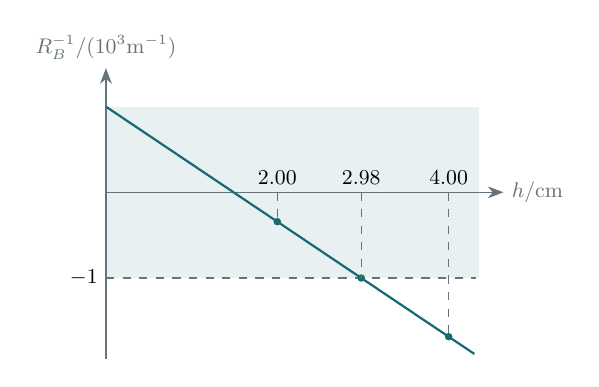
\begin{tikzpicture}[scale=.85,transform shape]
\begin{scope}[x=1.28cm,y=1.28cm]
\fill[accent!10](0,-1)rectangle(4.35,1);
\draw[axis](0,0)--(4.64,0)node[right]{$h/\mathrm{cm}$};
\draw[axis](0,-1.94)--(0,1.45)node[above]{$R_B^{-1}/(10^3\mathrm{m^{-1}})$};
\draw[guide](0,-1)--(4.32,-1);
\draw[traj,domain=0:4.3,samples=30]plot(\x,{1-.671232876712*\x});
\foreach \x/\y/\lab in {2/-.342466/2.00,2.98/-1.000274/2.98,4/-1.684932/4.00}{
\fill[accent](\x,\y)circle(1.6pt); \draw[guide](\x,0)--(\x,\y);
\node[above]at(\x,0){$\lab$};}
\node[left]at(0,-1){$-1$};
\end{scope}
\end{tikzpicture}
\figcaption{变图热4.5V1\quad 加倍管径后，阴影给下端球冠可采用的曲率范围}
\end{minipage}\end{center}
\item 求下端恰为平面时的高度。平面有 $p_B=p_0$，故沿变图热4.5V2的压力直线求零点。上端内侧比大气低292 Pa，液柱补回的压强是 $\rho gh$，所以 $h_c=292/(\rho g)=2.97959\,\mathrm{cm}$，按给定精度为2.98 cm。表面张力仍以原数值决定上端压降。
\begin{center}\begin{minipage}{.98\linewidth}\centering
\begin{tikzpicture}[scale=.85,transform shape]
\draw[axis](0,0)--(6.0,0)node[right]{$h$};
\draw[axis](0,-1.91)--(0,1.62)node[above]{$p_B-p_0$};
\draw[traj](0,-1.6)--(5.3,1.28);
\fill[accent](2.94444,0)circle(1.7pt);
\draw[guide](2.94444,0)--(2.94444,-.53);
\node[below]at(2.94444,-.53){$h_c=2.98\,\mathrm{cm}$};
\node[left]at(0,-1.6){$-292\,\mathrm{Pa}$};
\end{tikzpicture}
\figcaption{变图热4.5V2\quad 下端过零压差时，内外液面压强相同}
\end{minipage}\end{center}
\item 上端接触角为 $\theta_A$，从液体一侧量角。圆管内球面上端给 $R_A=r/\cos\theta_A$，于是 $h_c=2\sigma\cos\theta_A/(\rho gr)$。变图热4.5V3按零接触角时的 $h_{c0}$ 归一。若 $\theta_A=60^\circ$，上端压降减半，临界高度也减半。下端仍用题设的端口约束。
\begin{center}\begin{minipage}{.98\linewidth}\centering
\begin{tikzpicture}[scale=.85,transform shape]
\draw[axis](0,0)--(5.9,0)node[right]{$\theta_A$};
\draw[axis](0,0)--(0,2.9)node[above]{$h_c/h_{c0}$};
\draw[traj,domain=0:5.25,samples=73]plot(\x,{2.4*cos(90*\x/5.25)});
\fill[accent](3.5,1.2)circle(1.65pt);
\draw[guide](3.5,0)--(3.5,1.2)--(0,1.2);
\node[left]at(0,2.4){$1$};\node[left]at(0,1.2){$1/2$};
\node[below]at(3.5,0){$60^\circ$};\node[below]at(5.25,0){$90^\circ$};
\end{tikzpicture}
\figcaption{变图热4.5V3\quad 上端接触角改变其曲率压差及临界高度}
\end{minipage}\end{center}
\item 同一根管、同一重力条件下，$h_c$ 与 $\sigma/\rho$ 成正比。变图热4.5V4比较水与一种 $\sigma=0.060\,\mathrm{N/m}$、$\rho=800\,\mathrm{kg/m^3}$ 的液体，两者均取完全润湿。后一液体的 $\sigma/\rho=7.50\times10^{-5}\,\mathrm{m^3/s^2}$，略高于水的 $7.30\times10^{-5}\,\mathrm{m^3/s^2}$，临界高度因而为 $3.06\,\mathrm{cm}$。固定 $h$ 时，再用 $R_B^{-1}=r^{-1}(1-h/h_c)$ 判凹凸。
\begin{center}\begin{minipage}{.98\linewidth}\centering
\begin{tikzpicture}[scale=.85,transform shape]
\draw[axis](0,0)--(5.66,0)node[right]{液体};
\draw[axis](0,0)--(0,3.15)node[above]{$h_c/\mathrm{cm}$};
\fill[accent!28](.79,0)rectangle(1.82,2.384);
\fill[accent!54](2.95,0)rectangle(3.98,2.449);
\node[above]at(1.305,2.384){$2.98$};\node[above]at(3.465,2.449){$3.06$};
\node[below]at(1.305,0){水};\node[below]at(3.465,0){另一液体};
\end{tikzpicture}
\figcaption{变图热4.5V4\quad 改变液体时，临界高度由表面张力与密度之比决定}
\end{minipage}\end{center}
\item 令 $\delta h=h-h_c$。由曲率式得 $R_B^{-1}=-\rho g\delta h/(2\sigma)$，因此变图热4.5V5的曲率直线连续穿过原点。对应半径 $R_B=-2\sigma/(\rho g\delta h)$，当 $\delta h$ 从两侧趋向零，曲率都趋零，而半径的绝对值增大。
\begin{center}\begin{minipage}{.98\linewidth}\centering
\begin{tikzpicture}[scale=.85,transform shape]
\draw[axis](-3.15,0)--(3.35,0)node[right]{$\delta h/h_c$};
\draw[axis](0,-1.8)--(0,2.05)node[above]{$r/R_B$};
\draw[traj](-2.55,1.55)--(2.55,-1.55);
\fill[accent](0,0)circle(1.75pt);
\node[above left]at(-1.32,1.14){短柱，正曲率};
\node[below right]at(1.25,-1.07){长柱，负曲率};
\node[above right]at(.36,.16){平面};
\end{tikzpicture}
\figcaption{变图热4.5V5\quad 临界点上，曲率连续通过零}
\end{minipage}\end{center}
\item 两端外压分别为 $p_{0A},p_{0B}$。沿变图热4.5V6从上端外侧进入液体，过上液面后减 $2\sigma/R_A$，再向下加 $\rho gh$，所得 $p_B$ 与下端外压相减，得到
\[
\frac1{R_B}=\frac1{R_A}+\frac{p_{0B}-p_{0A}-\rho gh}{2\sigma}.
\]
提高下端外压时正曲率增加。平面条件改为 $\rho gh_c=2\sigma/R_A+(p_{0B}-p_{0A})$，取正柱高的解。
\begin{center}\begin{minipage}{.98\linewidth}\centering
\begin{tikzpicture}[scale=.85,transform shape]
\node[draw](O)at(0,1.65){$p_{0A}$};
\node[draw](A)at(2.45,1.65){$p_A$};
\node[draw](B)at(4.93,1.65){$p_B$};
\draw[motion](O.east)--(A.west)node[midway,above]{$-2\sigma/R_A$};
\draw[motion](A.east)--(B.west)node[midway,above]{$+\rho gh$};
\node[draw](P)at(4.93,.18){$p_{0B}$};
\draw[<->](B.south)--(P.north)node[midway,right]{$p_{0B}-p_B$};
\end{tikzpicture}
\figcaption{变图热4.5V6\quad 先求下端的液侧压强，再与该端自己的气侧压强比较}
\end{minipage}\end{center}
\item 若上、下接触线都能在同一圆管内自由移动，并在液体侧保持零接触角，变图热4.5V7中的两个弯月面都向水柱内部凹，球面半径均为 $r$。在同一外压 $p_0$ 下，两个液侧压强同为 $p_0-2\sigma/r$，静力条件给 $\rho gh=0$。因此这一自由接触线模型下没有正高度的静止柱。题中的三种静止高度利用下端钉扎改变曲率。
\begin{center}\begin{minipage}{.98\linewidth}\centering
\begin{tikzpicture}[scale=.85,transform shape]
\draw[object](0,0)--(0,3.15) (1.25,0)--(1.25,3.15);
\fill[accent!17](0,.42)arc[start angle=180,end angle=0,radius=.625]--(1.25,2.74)arc[start angle=0,end angle=-180,radius=.625]--cycle;
\draw[traj](0,.42)arc[start angle=180,end angle=0,radius=.625];
\draw[traj](0,2.74)arc[start angle=180,end angle=360,radius=.625];
\node at(.625,1.59){水};
\node[right]at(1.49,2.43){$p_A=p_0-2\sigma/r$};
\node[right]at(1.49,.72){$p_B=p_0-2\sigma/r$};
\node[left]at(-.08,2.87){空气 $p_0$};
\node[left]at(-.08,.18){空气 $p_0$};
\end{tikzpicture}
\figcaption{变图热4.5V7\quad 两端的半球都凹向水柱，液侧压强相同}
\end{minipage}\end{center}
\item 本题半径 $r=0.50\,\mathrm{mm}$，$\mathrm{Bo}=\rho gr^2/\sigma\simeq0.0336$。在单个弯月面尺度，重力压差与曲率压差之比 $\rho gr/(2\sigma/r)=\mathrm{Bo}/2\simeq0.0168$。变图热4.5V8再比较 $h=4.00\,\mathrm{cm}$ 的整体静水压，$\rho gh/(2\sigma/r)\simeq1.34$。单个弯月面近似球面，整柱计算仍保留重力。
\begin{center}\begin{minipage}{.98\linewidth}\centering
\begin{tikzpicture}[scale=.85,transform shape]
\draw[axis](0,0)--(5.73,0)node[right]{长度尺度};
\draw[axis](0,0)--(0,3.2)node[above]{$\rho g\ell/(2\sigma/r)$};
\fill[accent!32](.75,0)rectangle(1.65,.0353);
\fill[accent!55](3.17,0)rectangle(4.07,2.8192);
\node[above]at(1.2,.0353){$0.0168$};\node[above]at(3.62,2.8192){$1.34$};
\node[below]at(1.2,0){弯月面，$\ell=r$};
\node[below]at(3.62,0){整柱，$\ell=h$};
\end{tikzpicture}
\figcaption{变图热4.5V8\quad 整柱高度比管半径大，静水压随长度累积}
\end{minipage}\end{center}
\end{enumerate}

\clearpage

\pdfbookmark[2]{第 6 题 双液体U形毛细管表面张力比}{q6}

\section*{第 6 题\quad 双液体U形毛细管表面张力比}

总长$L$、内半径$R$均匀的倒U形毛细管，其两开口竖直向下，略浸入两种液体的等高液面。两液体密度$\rho_1,\rho_2$，与管壁接触角均为零；毛细管中气体不漏出，压缩过程等温，液体上升高度分别为$h_1,h_2$。插入前气体压强为大气压$p_0$，开口浸入深度忽略。求两液体表面张力系数$\sigma_1/\sigma_2$，并说明$h_1+h_2<L$的意义。

\begin{center}\begin{minipage}{0.96\linewidth}\centering\begin{tikzpicture}[x=1cm,y=1cm,font=\small,every node/.append style={align=center}]\fill[blue!15] (-.5,-.7) rectangle (1.8,.8);\fill[brown!15] (3.2,-.7) rectangle (5.5,.8);
\draw[object] (-.5,.8)--(1.8,.8);\draw[object] (3.2,.8)--(5.5,.8);
\draw[object] (.5,0)--(.5,3) .. controls (.5,3.5) and (4.5,3.5) ..(4.5,3)--(4.5,0);
\draw[object] (.8,0)--(.8,2.8) ..controls(.8,3.15) and(4.2,3.15)..(4.2,2.8)--(4.2,0);
\draw[traj] (.5,2.1)..controls(.6,1.95) and(.7,1.95)..(.8,2.1);
\draw[traj] (4.2,1.8)..controls(4.3,1.65) and(4.4,1.65)..(4.5,1.8);
\draw[<->] (1.3,.8)--(1.3,2.1) node[midway,right]{$h_1$};\draw[<->] (3.7,.8)--(3.7,1.8) node[midway,left]{$h_2$};
\node at (2.5,3.8){封闭气体$p$，长度$L-h_1-h_2$};\node at (.3,-.45){液体1};\node at (4.6,-.45){液体2};\end{tikzpicture}\figcaption{图 热4.6　倒U形管中的气体被两液柱共同压缩。}\end{minipage}\end{center}

\Needspace{5\baselineskip}

\pdfbookmark[3]{题型定位}{q6-h0}

\subsection*{题型定位}

两支液柱共同压缩倒U管中的气体。用气体压缩关系和两个液面压差求表面张力之比，再求有限表面张力允许的上升范围。

\Needspace{5\baselineskip}

\pdfbookmark[3]{知识点}{q6-h1}

\subsection*{知识点}

气体等温且密闭，$p(L-H)=p_0L$。每支液体的液侧压强为 $p_0-\rho_i gh_i$，跨完全润湿凹面的压强增量为 $2\sigma_i/R$。有限表面张力限制 $\Delta p$，两个上升高度之和因而有上界。


\Needspace{5\baselineskip}

\pdfbookmark[3]{物理图像}{q6-h2}

\subsection*{物理图像}

图热4.6两端液体挤压同一团气体，弯管也含在气柱长度中。解图热4.6B从槽面出发，沿每支液体向上减去静水压，跨凹面增加毛细压差，两条路径都到达同一气压。

\Needspace{5\baselineskip}

\pdfbookmark[3]{解题入口}{q6-h3}

\subsection*{解题入口}

令 $H=h_1+h_2$，用剩余长度 $L-H$ 得 $\Delta p$。对两端分别沿解图热4.6B写 $p=p_0-\rho_i gh_i+2\sigma_i/R$，相除消去 $R$。若要张力差，则将两式相减消去 $\Delta p$。


\Needspace{5\baselineskip}

\pdfbookmark[3]{标准解法}{q6-h4}

\subsection*{标准解法}

沿图热4.6的倒 U 形管，管道截面积恒定，两端液柱升起使气柱长度由 $L$ 减为 $L-h_1-h_2$。封闭气体取等温理想气体，管内两端的气体静压差约为 $\rho_{\rm gas}g|h_1-h_2|$，这里忽略这项，取共同气压 $p$，得到
\[
p(L-h_1-h_2)=p_0L,
\quad p=\frac{p_0L}{L-h_1-h_2},
\quad \Delta p=p-p_0=\frac{p_0(h_1+h_2)}{L-h_1-h_2}.
\]
在液体1内，毛细液面下方的压力也可由外界等高液面计算：
\[
p_{l1}=p_0-\rho_1gh_1.
\]
完全润湿的凹半球跨面压力关系为$p-p_{l1}=2\sigma_1/R$。液体2同理。因此
\[
\frac{2\sigma_1}{R}=\Delta p+\rho_1gh_1,\qquad
\frac{2\sigma_2}{R}=\Delta p+\rho_2gh_2.
\]
\begin{center}\begin{minipage}{0.96\linewidth}\centering\begin{tikzpicture}[x=1cm,y=1cm,font=\small,every node/.append style={align=center}]\node[draw] at (2.8,2.5){$p(L-h_1-h_2)=p_0L$};
\draw[object] (0,0)--(0,1.8);\draw[object] (.7,0)--(.7,1.8);\draw[traj] (0,1.5)..controls(.2,1.2) and(.5,1.2)..(.7,1.5);
\node[left] at (0,1.6){气体$p$};\node[right] at (.7,1){$p_{l1}=p_0-\rho_1gh_1$};
\node at (3.1,.1){$2\sigma_1/R=(p-p_0)+\rho_1gh_1$\\$2\sigma_2/R=(p-p_0)+\rho_2gh_2$};\end{tikzpicture}\figcaption{解图 热4.6A　两端共用同一压强增量，而静水项各自计算。}\end{minipage}\end{center}
解图热4.6A中，对任一支液体从槽外水平面走到管内气体，压力变化可按同一路径逐段相加：
\begin{center}\begin{minipage}{0.96\linewidth}\centering
\begin{tikzpicture}[x=1cm,y=1cm]
\node[draw,minimum width=1cm] (A) at (0,0) {$p_0$};
\node[draw,minimum width=1.2cm] (B) at (3.5,0) {$p_{li}$};
\node[draw,minimum width=1cm] (C) at (7,0) {$p$};
\draw[->,thick,color=accent] (A)--(B) node[midway,above] {$-\rho_i gh_i$};
\draw[->,thick,color=accent] (B)--(C) node[midway,above] {$+2\sigma_i/R$};
\node[below] at (1.7,-.15) {沿液体向上};\node[below] at (5.25,-.15) {跨凹液面};
\end{tikzpicture}
\figcaption{解图热4.6B\quad 两支液体各有自己的静水项，但终点为同一封闭气体压强。}
\end{minipage}\end{center}
沿解图热4.6B相加得$p=p_0-\rho_i gh_i+2\sigma_i/R$。因此毛细压差要承担气体增压和液柱重力两项，所以 $p-p_{li}=\Delta p+\rho_i gh_i$。

相除消去共同管半径，并代入封闭气体的增压项，得到
\[
\result{\frac{\sigma_1}{\sigma_2}
=\frac{p_0(h_1+h_2)+\rho_1gh_1(L-h_1-h_2)}
{p_0(h_1+h_2)+\rho_2gh_2(L-h_1-h_2)}}.
\]
气体若与大气连通，取 $p=p_0$，张力比为 $\rho_1h_1/(\rho_2h_2)$。题设给出的是两支通过同一个封闭气体耦合的平衡。

\textbf{封闭气柱长度与张力比的极限。} 等温压缩关系适用于封闭气柱仍有正长度的状态，即$h_1+h_2<L$。若$h_1=h_2$且$\rho_1=\rho_2$，两边静水项相等，张力比为1。固定两液柱高度比较时，增压项远大于两个静水项，张力比趋近1。改变$L$时，则由完整平衡方程联立求新的$h_1,h_2$。
\subsubsection*{共同增压对张力差和张力比的影响}
解图热4.6B的两条路径都从槽外$p_0$出发，以同一封闭气体p结束，
但两段液体的静水压降分别为$\rho_1gh_1$和$\rho_2gh_2$。
共同的$\Delta p$是两条毛细压差中的加数，只有相减才会消去：
\[
\frac{2(\sigma_1-\sigma_2)}R
=g(\rho_1h_1-\rho_2h_2).
\]
两种张力相等时，密度和高度的乘积相等。高度之比为两种密度的反比。
在张力比中，两侧毛细压差均含共同的加数 $\Delta p$。

令$H=h_1+h_2$、$\lambda=H/L$及$G_i=\rho_igh_i/p_0$，
答案可整理为
\[
\frac{\sigma_1}{\sigma_2}
=\frac{\lambda+(1-\lambda)G_1}
{\lambda+(1-\lambda)G_2},\qquad0<\lambda<1.
\]
这个表达式分开表示封闭气体压缩和两侧重力贡献。
开孔后的公式相当于气体增压为零，
要把闭气结果近似成开孔结果，须有$\Delta p\ll\rho_igh_i$对相关两侧都成立，
即使 $H/L$ 较小，也要比较这一压缩量与两侧静水项的实际量级。

\subsubsection*{剩余气体体积与有限张力的约束}
题图给定的是管长和测得高度，气体体积按统一截面积乘剩余长度计算。
这里忽略弯月面的端部体积和极小浸入深度，管子弯曲部分的长度已计入总长L。
若端部体积不可忽略，应直接用实际气体体积写$pV_g=p_0V_{g0}$，
实际气体体积包括弯管部分。两侧静水压仍按各自界面与槽面的竖直高度差计算。

由于两液体都上升，$\rho_igh_i>0$，有限的毛细压差要求
\[
\Delta p<\min\left(\frac{2\sigma_1}R,\frac{2\sigma_2}R\right)=c,
\qquad H<\frac{c}{p_0+c}L<L.
\]
每侧还有$h_i<2\sigma_i/(\rho_i gR)$。
有限表面张力给 $H<[c/(p_0+c)]L$，可达的上升总长早于气柱体积趋零。改变管长、排气状态或温度时，新的高度由气体和两支液柱的方程联立确定。


\Needspace{5\baselineskip}

\pdfbookmark[3]{关键洞察}{q6-h5}

\subsection*{关键洞察}

两支压缩气体所需的压差相同，支撑各自液柱所需的压差不同。两种张力恰相等时，$\rho_1h_1=\rho_2h_2$。当气体增压相对两侧静水项都很小，张力比接近开孔时的密度高度积之比。

\Needspace{5\baselineskip}

\pdfbookmark[3]{易错点}{q6-h6}

\subsection*{易错点}

气柱长度扣掉两支上升长度，弯管包含在总长内。静力项用竖直高度。张力比保留共同加数 $\Delta p$。改变几何或气体过程后重新联立两个液面高度。接触角改变时，保留各侧的 $\cos\theta_i$。

\Needspace{5\baselineskip}

\pdfbookmark[3]{课堂讲解建议}{q6-h7}

\subsection*{课堂讲解建议}

让学生沿解图热4.6B分别读两支的减压段和增压段，再在图热4.6把气体剩余长度写出来。比较张力差和张力比，问共同的气压在哪个运算中会消去。

再沿变图热4.6V1和V6比较开孔、封闭等温及封闭绝热的三种气体关系。改变管长时，在变图热4.6V3上说明交点怎样重新确定。最后以变图热4.6V7的水平线读有限毛细压差对 $H/L$ 的限制。

\Needspace{5\baselineskip}

\pdfbookmark[3]{变式训练}{q6-h8}

\subsection*{变式训练}

\begin{enumerate}
\item 若气体可缓慢逸出，平衡时 $p=p_0$。变图热4.6V1的排气孔使气体与大气等压，两侧静力和拉普拉斯式给 $2\sigma_i/R=\rho_i gh_i$，因此 $\sigma_1/\sigma_2=\rho_1h_1/(\rho_2h_2)$。开孔后实际高度由这两条新平衡式确定。
\begin{center}\begin{minipage}{.98\linewidth}\centering
\begin{tikzpicture}[scale=.85,transform shape]
\draw[object](0,0)--(0,2.75)--(2.15,2.75) (2.62,2.75)--(4.8,2.75)--(4.8,0);
\draw[object](.42,0)--(.42,2.32)--(4.38,2.32)--(4.38,0);
\draw[traj](0,1.45)..controls(.14,1.29)and(.28,1.29)..(.42,1.45);
\draw[traj](4.38,1.75)..controls(4.52,1.59)and(4.66,1.59)..(4.8,1.75);
\draw[motion](2.385,2.51)--(2.385,3.4)node[right]{排气孔};
\node[below]at(2.4,2.31){$p=p_0$};
\node[below]at(.21,0){液体1};\node[below]at(4.59,0){液体2};
\end{tikzpicture}
\figcaption{变图热4.6V1\quad 开孔后气体与大气连通，两支液体各由自身的静水项确定曲率压力}
\end{minipage}\end{center}
\item 若 $\rho_1=\rho_2=\rho$，比值化为 $(\Delta p+\rho gh_1)/(\Delta p+\rho gh_2)$。变图热4.6V2以 $h_1>h_2$ 为例，上推共同底段后，两个总高度的差仍为 $\rho g(h_1-h_2)$，所以 $\sigma_1>\sigma_2$。在等密度的条件下，$h_1=h_2$ 给 $\sigma_1/\sigma_2=1$。共同增压增加时，固定高度的两柱总高之比趋于1。
\begin{center}\begin{minipage}{.98\linewidth}\centering
\begin{tikzpicture}[scale=.85,transform shape]
\draw[axis](0,0)--(5.13,0)node[right]{支管};
\draw[axis](0,0)--(0,3.48)node[above]{$2\sigma_i/R$};
\foreach \x/\height/\i in {1.25/2.92/1,3.48/2.24/2}{
\fill[accent!25]({\x-.47},0)rectangle({\x+.47},1.27);
\fill[warm!30]({\x-.47},1.27)rectangle({\x+.47},\height);
\node at(\x,.6){$\Delta p$};
\node at(\x,{(\height+1.27)/2}){$\rho gh_{\i}$};
\node[below]at(\x,0){$\i$};}
\end{tikzpicture}
\figcaption{变图热4.6V2\quad 等密度时，两支毛细压差的差值由高度差决定}
\end{minipage}\end{center}
\item 增大总长 $L$ 时，如果先固定测得的 $H$，则 $p_0H/(L-H)$ 减小。对材料参数固定的实际装置，令 $C_i=2\sigma_i/R$，两侧方程相加给
\[
H=H_*-\mathcal B\Delta p,\quad
H_*=\frac1g\sum_i\frac{C_i}{\rho_i},\quad
\mathcal B=\frac1g\sum_i\frac1{\rho_i}.
\]
变图热4.6V3画出这条下降直线与两条气体曲线。$L$ 加长使同一 $\Delta p$ 下气体曲线 $H=L\Delta p/(p_0+\Delta p)$ 上移，交点的 $\Delta p$ 降低而 $H$ 增加。两液柱均上升时，再分别由 $(C_i-\Delta p)/(\rho_i g)$ 求高度。
\begin{center}\begin{minipage}{.98\linewidth}\centering
\begin{tikzpicture}[scale=.85,transform shape]
\draw[axis](0,0)--(5.88,0)node[right]{$\Delta p/p_0$};
\draw[axis](0,0)--(0,3.47)node[above]{$H$};
\draw[object](0,3.16)--(5.03,.51);
\draw[traj,domain=0:5.45,samples=76]plot(\x,{3.05*(\x/2)/(1+\x/2)});
\draw[object,dashed,domain=0:5.45,samples=76]plot(\x,{4.1*(\x/2)/(1+\x/2)});
\fill[accent](2.681851,1.747096)circle(1.5pt) (2.054552,2.077582)circle(1.5pt);
\node[above]at(4.78,2.18){较短管};
\node[above]at(4.68,2.96){较长管};
\node[above right]at(.59,2.84){液柱关系};
\node[below]at(2,0){$1$};
\end{tikzpicture}
\figcaption{变图热4.6V3\quad 管长改变时，在新的气体曲线上重新求与液柱直线的交点}
\end{minipage}\end{center}
\item 令 $G_i=\rho_i gh_i$。当 $\Delta p\gg G_i$ 对两侧都成立，
\[
\frac{\sigma_1}{\sigma_2}=1+\frac{G_1-G_2}{\Delta p+G_2}
=1+\frac{G_1-G_2}{\Delta p}+O\!\left(\frac{\max_iG_i^2}{(\Delta p)^2}\right).
\]
变图热4.6V4取 $G_1=2G_2$，画出比值随 $\Delta p/G_2$ 增大向1靠近。这一近似比较的是气体的增压 $\Delta p$ 和液柱静水项。
\begin{center}\begin{minipage}{.98\linewidth}\centering
\begin{tikzpicture}[scale=.85,transform shape]
\begin{scope}[x=.54cm,y=2.54cm]
\draw[axis](0,.86)--(10.34,.86)node[right]{$\Delta p/G_2$};
\draw[axis](0,.86)--(0,2.24)node[above]{$\sigma_1/\sigma_2$};
\draw[traj,domain=0:10,samples=95]plot(\x,{(\x+2)/(\x+1)});
\draw[guide](0,1)--(10,1);
\node[left]at(0,1){$1$};\node[left]at(0,2){$2$};
\node[below]at(0,.86){$0$};\node[below]at(10,.86){$10$};
\end{scope}
\end{tikzpicture}
\figcaption{变图热4.6V4\quad 增压项相对静水项变大时，张力比靠近1}
\end{minipage}\end{center}
\item 若两侧接触角不同，从各自液体内部量 $\theta_i$，使圆管凹面的曲率项为 $2\sigma_i\cos\theta_i/R$。由变图热4.6V5的两条压强路径，有
\[
\frac{\sigma_1}{\sigma_2}=
\frac{\Delta p+\rho_1gh_1}{\Delta p+\rho_2gh_2}
\frac{\cos\theta_2}{\cos\theta_1}.
\]
两液面都上升且 $\Delta p>0$ 时，各支的静水项与增压均为正，因而两接触角的余弦取正。
\begin{center}\begin{minipage}{.98\linewidth}\centering
\begin{tikzpicture}[scale=.85,transform shape]
\foreach \y/\i in {1.68/1,.28/2}{
\node[draw](A)at(0,\y){$p_0$};
\node[draw](B)at(2.7,\y){$p_{l\i}$};
\node[draw](C)at(5.72,\y){$p$};
\draw[motion](A.east)--(B.west)node[midway,above]{$-\rho_{\i}gh_{\i}$};
\draw[motion](B.east)--(C.west)node[midway,above]{$+2\sigma_{\i}\cos\theta_{\i}/R$};}
\end{tikzpicture}
\figcaption{变图热4.6V5\quad 不同接触角分别进入两条跨液面的压差}
\end{minipage}\end{center}
\item 若气体压缩近似准静态且对壁与液面的换热可略，以绝热式 $p(L-H)^\gamma=p_0L^\gamma$ 求 $p$。变图热4.6V6比较 $p/p_0=(1-H/L)^{-\gamma}$ 和等温关系。在相同压缩比例下，取 $\gamma>1$ 的绝热曲线给更高压力。将其减去 $p_0$ 后作为共同增压，再联立两支的静水与曲率方程。
\begin{center}\begin{minipage}{.98\linewidth}\centering
\begin{tikzpicture}[scale=.85,transform shape]
\begin{scope}[x=9cm,y=1.05cm]
\draw[axis](0,.72)--(.67,.72)node[right]{$H/L$};
\draw[axis](0,.72)--(0,4.16)node[above]{$p/p_0$};
\draw[traj,domain=0:.6,samples=84]plot(\x,{pow(1-\x,-1.4)});
\draw[object,dashed,domain=0:.6,samples=84]plot(\x,{1/(1-\x)});
\node[right]at(.45,2.59){绝热，$\gamma=1.4$};
\node[below]at(.43,1.75){等温};
\node[left]at(0,1){$1$};\node[below]at(.6,.72){$0.6$};
\end{scope}
\end{tikzpicture}
\figcaption{变图热4.6V6\quad 同一压缩比例下，绝热的气体压强高于等温值}
\end{minipage}\end{center}
\item 令 $\lambda=H/L$，封闭等温气体给 $\Delta p/p_0=\lambda/(1-\lambda)$。每支液体上升时都有 $\Delta p<C_i=2\sigma_i/R$。变图热4.6V7以 $c/p_0=1/2$ 为例，$c=\min(C_1,C_2)$，气体曲线与这条压差上限交于 $\lambda=1/3$。一般条件为 $\lambda<c/(p_0+c)$，所以在气体体积趋零之前，已先达到毛细压力所限的上升范围。
\begin{center}\begin{minipage}{.98\linewidth}\centering
\begin{tikzpicture}[scale=.85,transform shape]
\begin{scope}[x=6.8cm,y=1.5cm]
\draw[axis](0,0)--(.94,0)node[right]{$\lambda$};
\draw[axis](0,0)--(0,2.48)node[above]{$\Delta p/p_0$};
\draw[traj,domain=0:.69,samples=81]plot(\x,{\x/(1-\x)});
\draw[object,dashed](0,.5)--(.91,.5);
\fill[accent](.333333,.5)circle(1.8pt);
\draw[guide](.333333,0)--(.333333,.5);
\node[below]at(.333333,0){$1/3$};\node[below]at(.9,0){趋向1};
\node[right]at(.6,.5){$c/p_0=1/2$};
\end{scope}
\end{tikzpicture}
\figcaption{变图热4.6V7\quad 毛细压差的上限截断靠近剩余体积为零的气体曲线}
\end{minipage}\end{center}
\item 若两种表面张力均为 $\sigma$，设 $C=2\sigma/R$。由两式相减得 $\rho_1h_1=\rho_2h_2$。变图热4.6V8用等面积矩形表示相等的密度高度积，以 $\rho_2=2\rho_1$ 为例，此时 $h_1=2h_2$。总高确定后共同增压为 $p_0H/(L-H)$，还需满足
\[
C=\frac{p_0H}{L-H}+\frac{gH}{1/\rho_1+1/\rho_2}.
\]
右侧在 $0<H<L$ 随 $H$ 严格增加，解唯一。
\begin{center}\begin{minipage}{.98\linewidth}\centering
\begin{tikzpicture}[scale=.85,transform shape]
\draw[axis](0,0)--(5.8,0)node[right]{密度示意};
\draw[axis](0,0)--(0,2.94)node[above]{高度};
\fill[accent!30](.68,0)rectangle(1.72,2.36);
\fill[accent!45](2.88,0)rectangle(4.96,1.18);
\node[above]at(1.2,2.36){$h_1$};
\node[above]at(3.92,1.18){$h_2=h_1/2$};
\node[below]at(1.2,0){宽度 $\rho_1$};
\node[below]at(3.92,0){宽度 $2\rho_1$};
\end{tikzpicture}
\figcaption{变图热4.6V8\quad 等面积表示两侧的密度高度积相同}
\end{minipage}\end{center}
\end{enumerate}

\clearpage

\pdfbookmark[2]{第 7 题 微小水滴的曲率压强与密度变化}{q7}

\section*{第 7 题\quad 微小水滴的曲率压强与密度变化}

4℃、1 atm时水的表面张力$\sigma=7.24\times10^{-2}\,\mathrm{N/m}$，等温压缩系数$\beta=-(1/V)(\partial V/\partial p)_T=4.75\times10^{-5}\,\mathrm{atm^{-1}}$。同温、同外压下，平液面附近水的密度为$\rho_0$。求半径$r=1.0\times10^{-6}\,\mathrm{cm}$的微小水滴密度。计算中取$\sigma,\beta$为常量，并讨论该连续介质估算的条件。

\begin{center}\begin{minipage}{0.96\linewidth}\centering\begin{tikzpicture}[x=1cm,y=1cm,font=\small,every node/.append style={align=center}]\fill[blue!12] (0,0) circle (1.2);\draw[object] (0,0) circle (1.2);\draw[guide] (0,0)--(1.2,0) node[midway,above]{$r$};
\node at (0,-.45){$p,\rho$};\node at (2.2,1.2){外压$p_0$};\draw[force] (1.2,0)--(.84,0);
\draw[force] (-1.2,0)--(-.84,0);\node at (3,-.5){$p-p_0=2\sigma/r$};
\node[below] at (0,-1.22){箭头为张力在小曲面上的合力};\end{tikzpicture}\figcaption{图 热4.7　球形水滴只有一个界面，外压不是滴内压强。}\end{minipage}\end{center}

\Needspace{5\baselineskip}

\pdfbookmark[3]{题型定位}{q7-h0}

\subsection*{题型定位}

曲面两侧平衡给出附加压强，等温压缩关系把压力换成液体的密度变化。用同质量的体积与半径区分参考态和滴内状态。

\Needspace{5\baselineskip}

\pdfbookmark[3]{知识点}{q7-h1}

\subsection*{知识点}

球形单界面给 $\Delta p=2\sigma/r$，压缩系数为 $\beta=-V^{-1}(\partial V/\partial p)_T$。固定质量时 $\dd\ln\rho=-\dd\ln V$，等温积分给密度比。线性化由无量纲乘积 $z=\beta\Delta p$ 的大小决定。


\Needspace{5\baselineskip}

\pdfbookmark[3]{物理图像}{q7-h2}

\subsection*{物理图像}

题图热4.7中，若沿球心将液滴剖成两半，内外压差作用于圆盘 $\pi r^2$，表面张力沿圆周 $2\pi r$ 拉住半滴。体积压缩后保持同质量，滴内密度随之增大。解图热4.7A用曲线与切线表示指数解及其一次项。

\Needspace{5\baselineskip}

\pdfbookmark[3]{解题入口}{q7-h3}

\subsection*{解题入口}

先将厘米与大气压统一为米和帕，再由半球受力求滴内相对外界的压差。同一份水沿等温过程从 $p_0$ 积分到 $p_0+\Delta p$，把体积比倒过来得到密度比。算出 $z$ 后，再比较指数值与一次项。


\Needspace{5\baselineskip}

\pdfbookmark[3]{标准解法}{q7-h4}

\subsection*{标准解法}

图中液滴为单界面球面，滴内压强高于外压：$p-p_0=2\sigma/r$。压缩系数描述同一份水随压力的体积变化。在等温、$\beta$取常量时，
\[
\beta\dd p=-\frac{\dd V}{V},\qquad
\beta(p-p_0)=\ln\frac{V_0}{V}.
\]
同质量下$\rho V=\rho_0V_0$，于是
\[
\ln\frac{\rho}{\rho_0}=\beta(p-p_0),\qquad
\result{\rho=\rho_0\exp\left(\frac{2\sigma\beta}{r}\right)}.
\]
\begin{center}\begin{minipage}{0.96\linewidth}\centering\begin{tikzpicture}[x=4.7cm,y=1.35cm,font=\small]
\draw[axis] (0,0)--(1.2,0) node[right] {$z=2\sigma\beta/r$};
\draw[axis] (0,0)--(0,3.1) node[above] {$\rho/\rho_0$};
\draw[traj,domain=0:1,samples=100] plot(\x,{exp(\x)});
\draw[warm,thick,dashed,domain=0:1] plot(\x,{1+\x});
\foreach \x in {.5,1}{\draw (\x,-.04)--(\x,.04) node[below=3pt] {$\x$};}
\foreach \y in {1,2}{\draw (-.015,\y)--(.015,\y) node[left=3pt] {$\y$};}
\node[right] at (.82,2.7) {$e^z$};\node[right] at (.88,1.75) {$1+z$};
\end{tikzpicture}\figcaption{解图 热4.7A　先积分压缩系数，再用小指数作近似。}\end{minipage}\end{center}
指数关系使用的是同质量水的体积变化，而$r$是最终液滴的曲率半径。由质量守恒，
\[\frac{V}{V_0}=\frac{\rho_0}{\rho}=e^{-z},\qquad
\frac{r_0}{r}=\left(\frac{V_0}{V}\right)^{1/3}=e^{z/3},\quad
z=\frac{2\sigma\beta}{r}.\]
其中 $r_0$ 表示同质量水在外压 $p_0$ 下的参考半径。拉普拉斯压差按实际液面的曲率半径 $r$ 计算。题图热4.7的箭头表示液面小面元所受张力的向内合力。张力沿小面元的边缘作切向牵引，曲率使这些牵引有向内的合量；内外压差提供向外的平衡力。内压升高使同质量的水体积减小、密度增大，即 $V<V_0$、$\rho>\rho_0$。

数值计算先统一单位：
\[
r=1.0\times10^{-6}\,\mathrm{cm}=1.0\times10^{-8}\,\mathrm m,
\quad \beta=\frac{4.75\times10^{-5}}{101325}\,\mathrm{Pa^{-1}}
=4.68789\times10^{-10}\,\mathrm{Pa^{-1}}.
\]
曲率压差及无量纲指数为
\[
\Delta p=\frac{0.1448}{10^{-8}}=1.448\times10^7\,\mathrm{Pa},
\quad z=\beta\Delta p=6.78806\times10^{-3}.
\]
所以
\[
\frac{\rho}{\rho_0}=e^z=1.006811,
\quad \rho\simeq\rho_0(1+z)=1.006788\rho_0\simeq1.0068\rho_0.
\]
密度约增加0.68\%。曲率压差约143 atm，仍只造成小相对密度变化，原因是水的压缩系数很小。把指数保留到一次项，相对于总密度的误差约为 $z^2/2=2.3\times10^{-5}$。这里把 $10\,\mathrm{nm}$ 液滴视为连续液体，并在所用压差内取常量 $\beta$ 和 $\sigma$。
\subsubsection*{半球受力、压缩量与线性近似}
将题图热4.7中的液滴沿过球心平面剖成两半，
内外压力差在圆截面上的合力为$\Delta p\,\pi r^2$，
球面张力沿周长$2\pi r$的合力为$2\pi r\sigma$。
平衡给$\Delta p=2\sigma/r$，方向指向滴外的内压与收缩液面的表面张力相抵。
半球圆周和截面都由同一个实际半径决定，所以周长除以面积正比于 $1/r$。

在积分中，$\dd V/V=-\dd\rho/\rho$来自质量不变，
因此压缩系数也可写成$\beta=(1/\rho)(\partial\rho/\partial p)_T$。
积分从外压$p_0$起，到滴内压$p_0+2\sigma/r$止。压强升高使密度增加，固定质量的体积相应减小。
本题数值还给$V/V_0\simeq0.993235$及$r_0/r\simeq1.002265$，
体积缩小约 $0.677\%$。由 $r/r_0=e^{-z/3}$ 得半径缩小约 $0.226\%$，约为体积相对变化量的三分之一。

解图热4.7A同时画$e^z$与$1+z$，两曲线在$z=0$相切，
正指数时指数曲线始终在切线上方，所以一阶式略低估密度。
本题$z\simeq0.006788$，两式差为密度基准的约$2.31\times10^{-5}$，
相对于精确密度的误差约$2.29\times10^{-5}$；
若所求量是密度增量，以 $e^z-1$ 作分母，得到的相对误差约为 $z/2=0.34\%$。
两个相对误差的分母分别是精确总密度和密度增加量，后者较小，因此相对误差较大。
如果题目改为给定同质量在外压下的半径$r_0$，
则用质量关系$\rho/\rho_0=(r_0/r)^3$与曲率压差联立求实际半径$r$，再代入密度指数式。


\Needspace{5\baselineskip}

\pdfbookmark[3]{关键洞察}{q7-h5}

\subsection*{关键洞察}

压差约143个大气压，水的小压缩系数却使 $z\simeq0.006788$。同一个截断量，以总密度和以密度增量为分母时，相对误差约为 $2.29\times10^{-5}$ 和 $0.34\%$。这里的压缩关系采用连续液体及常物性参数，材料描述的精度由这些近似决定。若给的是 $r_0$，曲率压差和质量关系共同确定实际半径。

\Needspace{5\baselineskip}

\pdfbookmark[3]{易错点}{q7-h6}

\subsection*{易错点}

厘米换成米使半径的数值乘 $10^{-2}$，以大气压倒数给出的 $\beta$ 除以101325后可与帕相乘。水滴只有一层气液界面。质量守恒使 $\dd V/V$ 与 $\dd\rho/\rho$ 异号，所以增压导致增密。区分实际曲率半径、参考半径以及总密度和密度增量两个误差分母。

\Needspace{5\baselineskip}

\pdfbookmark[3]{课堂讲解建议}{q7-h7}

\subsection*{课堂讲解建议}

从半球受力开始。请学生在题图热4.7指出压力合力所用的圆盘和张力合力所用的圆周，各写出面积、周长，再说明为何压差随滴径减小而增大。用质量守恒把压缩系数改写成密度微分后，先报143个大气压，再报约 $0.68\%$ 的密度变化，解释中间相乘的小参数。

在解图热4.7A上指出 $e^z$ 与 $1+z$ 的差是同一段纵向间隔。分别以指数曲线的总高度和它高于 $\rho/\rho_0=1$ 的高度作参照，说明两种误差为什么相差两个数量级。接着把给定半径换成参考半径，让学生用质量关系与拉普拉斯式联立。

\Needspace{5\baselineskip}

\pdfbookmark[3]{变式训练}{q7-h8}

\subsection*{变式训练}

\begin{enumerate}
\item 半径由 $r_*$ 增至 $10r_*$，曲率压差从 $2\sigma/r_*$ 降至其十分之一。变图热4.7V1两标点的纵坐标也是 $z/z_*$，因为压缩系数固定。取题给物性参数，十倍半径给 $e^{z_*/10}-1\simeq6.7904\times10^{-4}$，密度增加约 $0.06790\%$。一次近似下，密度增量同样随半径的倒数变化。
\begin{center}\begin{minipage}{.98\linewidth}\centering
\begin{tikzpicture}[scale=.85,transform shape]
\begin{scope}[x=.58cm,y=2.7cm]
\draw[axis](0,0)--(10.82,0)node[right]{$r/r_*$};
\draw[axis](0,0)--(0,1.16)node[above]{$\Delta p/\Delta p_*$};
\draw[traj,domain=1:10,samples=90]plot(\x,{1/\x});
\draw[guide](1,0)--(1,1)--(0,1) (10,0)--(10,.1)--(0,.1);
\fill[accent](1,1)circle(1.6pt) (10,.1)circle(1.6pt);
\node[below]at(1,0){$1$};\node[below]at(10,0){$10$};
\node[left]at(0,1){$1$};\node[left]at(0,.1){$0.1$};
\end{scope}
\end{tikzpicture}
\figcaption{变图热4.7V1\quad 曲率压差与半径成反比，定压缩系数下 $z/z_*=\Delta p/\Delta p_*$}
\end{minipage}\end{center}
\item 把水滴改成浸在液体中的单个气泡。沿变图热4.7V2由自由液面降到泡心深度 $d$，泡外压力为 $p_0+\rho_\ell gd$。气泡足够小，取泡面附近液体压强为同一值。跨一个球面进入泡内，再加 $2\sigma/r$。若气体可作理想气体，摩尔质量为 $\mu$，则
\[
\rho_{\rm g}=\frac{\mu}{RT}\left(p_0+\rho_\ell gd+\frac{2\sigma}{r}\right).
\]
\begin{center}\begin{minipage}{.98\linewidth}\centering
\begin{tikzpicture}[scale=.85,transform shape]
\fill[accent!13](0,-2.65)rectangle(5.5,0);
\draw[object](0,-2.65)--(0,0)--(5.5,0)--(5.5,-2.65)--cycle;
\filldraw[fill=white,draw=accent,thick](3.72,-1.46)circle(.53);
\draw[guide](1.08,-1.46)--(3.19,-1.46);
\draw[object,<->](1.08,0)--(1.08,-1.46)node[midway,left]{$d$};
\draw[object,<->](3.72,-1.46)--(3.72,-.93)node[midway,right]{$r$};
\draw[motion](2.82,-1.88)--(3.38,-1.69);
\node[below]at(3.72,-2.00){$p_{\rm g}$};
\node[left]at(2.93,-2.02){$p_0+\rho_\ell gd$};
\node[above]at(2.6,0){$p_0$};
\end{tikzpicture}
\figcaption{变图热4.7V2\quad 静水压力取在气泡处，球面内侧压强另加 $2\sigma/r$}
\end{minipage}\end{center}
\item 令测得的密度比为 $1+\delta$，取正值 $\delta$，则 $z=\ln(1+\delta)$，实际半径为
\[
r=\frac{2\sigma\beta}{\ln(1+\delta)}
=\frac{2\sigma\beta}{\delta}\left[1+\frac{\delta}{2}+O(\delta^2)\right].
\]
变图热4.7V3在相同增量 $\delta$ 下画两种反求半径。由于 $\ln(1+\delta)<\delta$，倒数形式的一阶值偏小。以 $\delta=0.01$ 为例，先将 $\beta$ 换为 $\mathrm{Pa^{-1}}$，再代入得到 $r\simeq6.82\,\mathrm{nm}$，一次值约 $6.79\,\mathrm{nm}$。
\begin{center}\begin{minipage}{.98\linewidth}\centering
\begin{tikzpicture}[scale=.85,transform shape]
\begin{scope}[x=5.7cm,y=.25cm]
\draw[axis](0,0)--(1.10,0)node[right]{$\delta$};
\draw[axis](0,0)--(0,12.46)node[above]{$r/(2\sigma\beta)$};
\draw[traj,domain=.09:1,samples=90]plot(\x,{1/ln(1+\x)});
\draw[object,dashed,domain=.09:1,samples=90]plot(\x,{1/\x});
\node[right]at(.26,6.5){$1/\ln(1+\delta)$};
\draw[guide](.26,6.5)--(.20,5.4848);
\node[below]at(.54,1.48){$1/\delta$};
\node[below]at(1,0){$1$};
\end{scope}
\end{tikzpicture}
\figcaption{变图热4.7V3\quad 由密度增量反求半径，双曲线近似偏低}
\end{minipage}\end{center}
\item 在固定 $r,\sigma$ 下令 $\beta\to0$，拉普拉斯压差仍为 $2\sigma/r$。变图热4.7V4中两个压强平台相差 $\Delta p$。同一份水在参考外压和滴内压力下的密度均为 $\rho_0$。由 $V=V_0e^{-\beta\Delta p}$ 也可见，不可压极限给 $V=V_0$。
\begin{center}\begin{minipage}{.98\linewidth}\centering
\begin{tikzpicture}[scale=.85,transform shape]
\draw[axis](0,0)--(5.12,0)node[right]{位置};
\draw[axis](0,0)--(0,2.9)node[above]{$p$};
\draw[traj](.39,.65)--(2.46,.65) (2.46,2.14)--(4.82,2.14);
\draw[guide](2.46,0)--(2.46,2.14);
\draw[object,<->](3.58,.65)--(3.58,2.14)node[midway,right]{$2\sigma/r$};
\node[left]at(0,.65){$p_0$};\node[left]at(0,2.14){$p_0+\Delta p$};
\node[below]at(2.46,0){液面};
\node[above]at(1.05,.69){滴外};\node[above]at(4.19,2.22){滴内，$\rho=\rho_0$};
\draw[guide](.5,.26)--(4.71,.26);
\node[fill=white]at(2.46,.26){$\beta=0$};
\end{tikzpicture}
\figcaption{变图热4.7V4\quad 不可压极限下，压差仍由界面曲率决定}
\end{minipage}\end{center}
\item 若等温压缩系数随压力变，仍在 $p_0\le p'\le p_0+2\sigma/r$ 上积分
\[
\ln\frac{\rho}{\rho_0}=\int_{p_0}^{p_0+2\sigma/r}\beta(p')\,\dd p'.
\]
变图热4.7V5以 $\beta(p')=\beta_0[1+\eta(p'-p_0)/\Delta p]$、$\eta=-0.3$ 示范。当 $\eta>-1$ 时，梯形面积为 $\beta_0\Delta p(1+\eta/2)$。图中参数给的指数为常值模型的 $0.85$ 倍。对具体液体，面积由给定的等温 $\beta(p')$ 曲线确定。
\begin{center}\begin{minipage}{.98\linewidth}\centering
\begin{tikzpicture}[scale=.85,transform shape]
\begin{scope}[x=4.9cm,y=2.32cm]
\fill[accent!20](0,0)--(0,1)--(1,.7)--(1,0)--cycle;
\draw[axis](0,0)--(1.17,0)node[right]{$p'$};
\draw[axis](0,0)--(0,1.25)node[above]{$\beta(p')$};
\draw[traj](0,1)--(1,.7);
\draw[guide](1,0)--(1,1)--(0,1);
\node[left]at(0,1){$\beta_0$};\node[right]at(1,.7){$0.7\beta_0$};
\node[below]at(0,0){$p_0$};\node[below]at(1,0){$p_0+\Delta p$};
\node at(.46,.38){$\beta_0\Delta p(1+\eta/2)$};
\end{scope}
\end{tikzpicture}
\figcaption{变图热4.7V5\quad 梯形面积是密度比的对数}
\end{minipage}\end{center}
\item 变图热4.7V6按米标出两种代入值。厘米数乘 $10^{-2}$ 后得到实际的 $10^{-8}\,\mathrm m$，而 $10^{-6}\,\mathrm m$ 对应 $100$ 倍半径。代入较大的数，曲率压差及指数都变为正确数值的 $1/100$，密度增量由 $e^z-1\simeq6.8111\times10^{-3}$ 变成 $e^{z/100}-1\simeq6.7883\times10^{-5}$，即由约 $0.68\%$ 降为 $0.0068\%$。
\begin{center}\begin{minipage}{.98\linewidth}\centering
\begin{tikzpicture}[scale=.85,transform shape]
\draw[axis](0,0)--(6.17,0)node[right]{$r\;(\mathrm m)$};
\foreach \x/\k in {1/-8,3/-7,5/-6}{
\draw[object](\x,-.08)--(\x,.08);
\node[below]at(\x,-.08){$10^{\k}$};}
\draw[guide](1,.11)--(1,1.37) (5,.11)--(5,1.37);
\draw[motion](1,1.18)--(5,1.18)node[midway,above]{$r$ 乘100};
\node[above]at(1,1.47){$10^{-6}\,\mathrm{cm}$};
\node[above]at(5,1.47){当作米};
\draw[motion](1,-1.04)--(5,-1.04)node[midway,below]{$z$ 除以100};
\end{tikzpicture}
\figcaption{变图热4.7V6\quad 横轴采用对数刻度，两次幂对应半径相差100倍}
\end{minipage}\end{center}
\item 对 $z>0$，一次式少计的密度为 $\rho_0[e^z-1-z]$。变图热4.7V7对比曲线和切线到参考线的高度，放大了 $z$ 以显示两者之差。对题中 $z=0.00678806$，该差为约 $2.31\times10^{-5}\rho_0$。除以总密度 $\rho_0e^z$ 得 $2.29\times10^{-5}$，除以密度增量 $\rho_0(e^z-1)$ 得约 $0.339\%$。若所求精度涉及纳米液滴物性，表面张力和压缩系数可按已知的相应尺度数据代入。
\begin{center}\begin{minipage}{.98\linewidth}\centering
\begin{tikzpicture}[scale=.85,transform shape]
\begin{scope}[x=5.9cm,y=1.67cm]
\draw[axis](0,0)--(1.03,0)node[right]{$z$};
\draw[axis](0,0)--(0,2.82)node[above]{$\rho/\rho_0$};
\draw[guide](0,1)--(.97,1);
\draw[traj,domain=0:.9,samples=75]plot(\x,{exp(\x)});
\draw[object,dashed](0,1)--(.9,1.9);
\draw[guide](.69,0)--(.69,1.99372);
\draw[guide](.69,1.69)--(.745,1.69) (.69,1.99372)--(.745,1.99372);
\draw[object,<->](.745,1.69)--(.745,1.99372)node[right]{$e^z-1-z$};
\node[left]at(0,1){$1$};\node[above]at(.85,2.36){$e^z$};
\node[below]at(.83,1.79){$1+z$};
\end{scope}
\end{tikzpicture}
\figcaption{变图热4.7V7\quad 曲线与切线之差用于计算截断误差，两个相对误差使用不同参照高}
\end{minipage}\end{center}
\item 若已知的是参考半径 $r_0$，同质量给 $\rho/\rho_0=(r_0/r)^3$。令 $C=2\sigma\beta$，联立得
\[
3\ln(r_0/r)=C/r,\qquad 3w\ln(1/w)=C/r_0,\quad w=r/r_0.
\]
变图热4.7V8上，左式对 $w$ 的导数为 $3[\ln(1/w)-1]$，在 $w=1/e$ 为零，峰值为 $3/e$。因此 $0<C/r_0<3/e$ 时有两个代数根。左支 $w<1/e$ 对应 $\rho/\rho_0>e^3$；图中小压缩所取的是靠近 $w=1$ 的右支。令 $w=1-\epsilon$，左侧展开为 $3\epsilon+O(\epsilon^2)$，所以 $r=r_0-C/3+O(C^2/r_0)$。
\begin{center}\begin{minipage}{.98\linewidth}\centering
\begin{tikzpicture}[scale=.85,transform shape]
\begin{scope}[x=5.8cm,y=2.15cm]
\draw[axis](0,0)--(1.1,0)node[right]{$w=r/r_0$};
\draw[axis](0,0)--(0,1.25)node[above]{$3w\ln(1/w)$};
\draw[traj](0,0)--(.002,.03729);
\draw[traj,domain=.002:1,samples=105]plot(\x,{3*\x*ln(1/\x)});
\draw[guide](.367879,0)--(.367879,1.103638);
\draw[object,dashed](0,.22)--(.99,.22);
\fill[accent](0.923677,.22)circle(1.8pt);
\node[above right]at(.915,.27){小压缩支};
\node[left]at(0,.22){$C/r_0$};
\node[below]at(.367879,0){$1/e$};\node[below]at(1,0){$1$};
\end{scope}
\end{tikzpicture}
\figcaption{变图热4.7V8\quad 压差关系与质量关系联立，取实际半径接近参考半径的一支}
\end{minipage}\end{center}
\end{enumerate}

\clearpage

\pdfbookmark[2]{第 8 题 相通肥皂泡的稳定与不稳定平衡}{q8}

\section*{第 8 题\quad 相通肥皂泡的稳定与不稳定平衡}

两相同球冠形肥皂泡A、B固定在半径$r_1$相同的圆管口上；外界压强相同，两泡连通，外部供气阀K关闭，连接泡的阀门保持开启。表面张力系数恒定，忽略液膜厚度和气体密度变化。证明：两泡均小于半球时等形平衡稳定，均大于半球时等形平衡不稳定。后一情形取$r_1=2.00\,\mathrm{cm}$、初始球面曲率半径$r_2=2.50\,\mathrm{cm}$，求一泡变小、另一泡变大后再次平衡的曲率半径与球冠高度。

\begin{center}\begin{minipage}{0.96\linewidth}\centering\begin{tikzpicture}[x=1cm,y=1cm,font=\small,every node/.append style={align=center}]\draw[traj] (-0.7500,0.0000) -- (-0.7389,0.0201) -- (-0.7273,0.0399) -- (-0.7151,0.0594) -- (-0.7025,0.0786) -- (-0.6893,0.0974) -- (-0.6756,0.1158) -- (-0.6614,0.1339) -- (-0.6467,0.1516) -- (-0.6316,0.1688) -- (-0.6160,0.1857) -- (-0.6000,0.2021) -- (-0.5835,0.2181) -- (-0.5666,0.2336) -- (-0.5492,0.2487) -- (-0.5315,0.2633) -- (-0.5134,0.2774) -- (-0.4949,0.2911) -- (-0.4761,0.3042) -- (-0.4569,0.3168) -- (-0.4373,0.3289) -- (-0.4175,0.3404) -- (-0.3973,0.3514) -- (-0.3769,0.3619) -- (-0.3561,0.3718) -- (-0.3352,0.3811) -- (-0.3139,0.3899) -- (-0.2925,0.3981) -- (-0.2708,0.4057) -- (-0.2489,0.4127) -- (-0.2269,0.4192) -- (-0.2047,0.4250) -- (-0.1823,0.4302) -- (-0.1598,0.4348) -- (-0.1372,0.4389) -- (-0.1145,0.4423) -- (-0.0917,0.4450) -- (-0.0688,0.4472) -- (-0.0459,0.4488) -- (-0.0230,0.4497) -- (0.0000,0.4500) -- (0.0230,0.4497) -- (0.0459,0.4488) -- (0.0688,0.4472) -- (0.0917,0.4450) -- (0.1145,0.4423) -- (0.1372,0.4389) -- (0.1598,0.4348) -- (0.1823,0.4302) -- (0.2047,0.4250) -- (0.2269,0.4192) -- (0.2489,0.4127) -- (0.2708,0.4057) -- (0.2925,0.3981) -- (0.3139,0.3899) -- (0.3352,0.3811) -- (0.3561,0.3718) -- (0.3769,0.3619) -- (0.3973,0.3514) -- (0.4175,0.3404) -- (0.4373,0.3289) -- (0.4569,0.3168) -- (0.4761,0.3042) -- (0.4949,0.2911) -- (0.5134,0.2774) -- (0.5315,0.2633) -- (0.5492,0.2487) -- (0.5666,0.2336) -- (0.5835,0.2181) -- (0.6000,0.2021) -- (0.6160,0.1857) -- (0.6316,0.1688) -- (0.6467,0.1516) -- (0.6614,0.1339) -- (0.6756,0.1158) -- (0.6893,0.0974) -- (0.7025,0.0786) -- (0.7151,0.0594) -- (0.7273,0.0399) -- (0.7389,0.0201) -- (0.7500,0.0000);\draw[object] (-0.75,0)--(-.2,0) (.2,0)--(.75,0);\draw[traj] (2.2500,0.0000) -- (2.2611,0.0201) -- (2.2727,0.0399) -- (2.2849,0.0594) -- (2.2975,0.0786) -- (2.3107,0.0974) -- (2.3244,0.1158) -- (2.3386,0.1339) -- (2.3533,0.1516) -- (2.3684,0.1688) -- (2.3840,0.1857) -- (2.4000,0.2021) -- (2.4165,0.2181) -- (2.4334,0.2336) -- (2.4508,0.2487) -- (2.4685,0.2633) -- (2.4866,0.2774) -- (2.5051,0.2911) -- (2.5239,0.3042) -- (2.5431,0.3168) -- (2.5627,0.3289) -- (2.5825,0.3404) -- (2.6027,0.3514) -- (2.6231,0.3619) -- (2.6439,0.3718) -- (2.6648,0.3811) -- (2.6861,0.3899) -- (2.7075,0.3981) -- (2.7292,0.4057) -- (2.7511,0.4127) -- (2.7731,0.4192) -- (2.7953,0.4250) -- (2.8177,0.4302) -- (2.8402,0.4348) -- (2.8628,0.4389) -- (2.8855,0.4423) -- (2.9083,0.4450) -- (2.9312,0.4472) -- (2.9541,0.4488) -- (2.9770,0.4497) -- (3.0000,0.4500) -- (3.0230,0.4497) -- (3.0459,0.4488) -- (3.0688,0.4472) -- (3.0917,0.4450) -- (3.1145,0.4423) -- (3.1372,0.4389) -- (3.1598,0.4348) -- (3.1823,0.4302) -- (3.2047,0.4250) -- (3.2269,0.4192) -- (3.2489,0.4127) -- (3.2708,0.4057) -- (3.2925,0.3981) -- (3.3139,0.3899) -- (3.3352,0.3811) -- (3.3561,0.3718) -- (3.3769,0.3619) -- (3.3973,0.3514) -- (3.4175,0.3404) -- (3.4373,0.3289) -- (3.4569,0.3168) -- (3.4761,0.3042) -- (3.4949,0.2911) -- (3.5134,0.2774) -- (3.5315,0.2633) -- (3.5492,0.2487) -- (3.5666,0.2336) -- (3.5835,0.2181) -- (3.6000,0.2021) -- (3.6160,0.1857) -- (3.6316,0.1688) -- (3.6467,0.1516) -- (3.6614,0.1339) -- (3.6756,0.1158) -- (3.6893,0.0974) -- (3.7025,0.0786) -- (3.7151,0.0594) -- (3.7273,0.0399) -- (3.7389,0.0201) -- (3.7500,0.0000);\draw[object] (2.25,0)--(2.8,0) (3.2,0)--(3.75,0);\draw[traj] (-0.7500,-3.0000) -- (-0.7800,-2.9576) -- (-0.8076,-2.9137) -- (-0.8327,-2.8683) -- (-0.8552,-2.8215) -- (-0.8752,-2.7736) -- (-0.8924,-2.7247) -- (-0.9069,-2.6749) -- (-0.9187,-2.6243) -- (-0.9276,-2.5732) -- (-0.9337,-2.5217) -- (-0.9369,-2.4699) -- (-0.9373,-2.4180) -- (-0.9348,-2.3662) -- (-0.9294,-2.3146) -- (-0.9212,-2.2633) -- (-0.9101,-2.2126) -- (-0.8963,-2.1626) -- (-0.8797,-2.1135) -- (-0.8604,-2.0653) -- (-0.8385,-2.0182) -- (-0.8140,-1.9725) -- (-0.7871,-1.9282) -- (-0.7577,-1.8854) -- (-0.7260,-1.8443) -- (-0.6920,-1.8051) -- (-0.6560,-1.7677) -- (-0.6179,-1.7325) -- (-0.5780,-1.6994) -- (-0.5362,-1.6685) -- (-0.4929,-1.6400) -- (-0.4480,-1.6140) -- (-0.4017,-1.5904) -- (-0.3543,-1.5695) -- (-0.3057,-1.5512) -- (-0.2562,-1.5357) -- (-0.2059,-1.5229) -- (-0.1550,-1.5129) -- (-0.1036,-1.5057) -- (-0.0519,-1.5014) -- (0.0000,-1.5000) -- (0.0519,-1.5014) -- (0.1036,-1.5057) -- (0.1550,-1.5129) -- (0.2059,-1.5229) -- (0.2562,-1.5357) -- (0.3057,-1.5512) -- (0.3543,-1.5695) -- (0.4017,-1.5904) -- (0.4480,-1.6140) -- (0.4929,-1.6400) -- (0.5362,-1.6685) -- (0.5780,-1.6994) -- (0.6179,-1.7325) -- (0.6560,-1.7677) -- (0.6920,-1.8051) -- (0.7260,-1.8443) -- (0.7577,-1.8854) -- (0.7871,-1.9282) -- (0.8140,-1.9725) -- (0.8385,-2.0182) -- (0.8604,-2.0653) -- (0.8797,-2.1135) -- (0.8963,-2.1626) -- (0.9101,-2.2126) -- (0.9212,-2.2633) -- (0.9294,-2.3146) -- (0.9348,-2.3662) -- (0.9373,-2.4180) -- (0.9369,-2.4699) -- (0.9337,-2.5217) -- (0.9276,-2.5732) -- (0.9187,-2.6243) -- (0.9069,-2.6749) -- (0.8924,-2.7247) -- (0.8752,-2.7736) -- (0.8552,-2.8215) -- (0.8327,-2.8683) -- (0.8076,-2.9137) -- (0.7800,-2.9576) -- (0.7500,-3.0000);\draw[object] (-0.75,-3)--(-.2,-3) (.2,-3)--(.75,-3);\draw[traj] (2.2500,-3.0000) -- (2.2200,-2.9576) -- (2.1924,-2.9137) -- (2.1673,-2.8683) -- (2.1448,-2.8215) -- (2.1248,-2.7736) -- (2.1076,-2.7247) -- (2.0931,-2.6749) -- (2.0813,-2.6243) -- (2.0724,-2.5732) -- (2.0663,-2.5217) -- (2.0631,-2.4699) -- (2.0627,-2.4180) -- (2.0652,-2.3662) -- (2.0706,-2.3146) -- (2.0788,-2.2633) -- (2.0899,-2.2126) -- (2.1037,-2.1626) -- (2.1203,-2.1135) -- (2.1396,-2.0653) -- (2.1615,-2.0182) -- (2.1860,-1.9725) -- (2.2129,-1.9282) -- (2.2423,-1.8854) -- (2.2740,-1.8443) -- (2.3080,-1.8051) -- (2.3440,-1.7677) -- (2.3821,-1.7325) -- (2.4220,-1.6994) -- (2.4638,-1.6685) -- (2.5071,-1.6400) -- (2.5520,-1.6140) -- (2.5983,-1.5904) -- (2.6457,-1.5695) -- (2.6943,-1.5512) -- (2.7438,-1.5357) -- (2.7941,-1.5229) -- (2.8450,-1.5129) -- (2.8964,-1.5057) -- (2.9481,-1.5014) -- (3.0000,-1.5000) -- (3.0519,-1.5014) -- (3.1036,-1.5057) -- (3.1550,-1.5129) -- (3.2059,-1.5229) -- (3.2562,-1.5357) -- (3.3057,-1.5512) -- (3.3543,-1.5695) -- (3.4017,-1.5904) -- (3.4480,-1.6140) -- (3.4929,-1.6400) -- (3.5362,-1.6685) -- (3.5780,-1.6994) -- (3.6179,-1.7325) -- (3.6560,-1.7677) -- (3.6920,-1.8051) -- (3.7260,-1.8443) -- (3.7577,-1.8854) -- (3.7871,-1.9282) -- (3.8140,-1.9725) -- (3.8385,-2.0182) -- (3.8604,-2.0653) -- (3.8797,-2.1135) -- (3.8963,-2.1626) -- (3.9101,-2.2126) -- (3.9212,-2.2633) -- (3.9294,-2.3146) -- (3.9348,-2.3662) -- (3.9373,-2.4180) -- (3.9369,-2.4699) -- (3.9337,-2.5217) -- (3.9276,-2.5732) -- (3.9187,-2.6243) -- (3.9069,-2.6749) -- (3.8924,-2.7247) -- (3.8752,-2.7736) -- (3.8552,-2.8215) -- (3.8327,-2.8683) -- (3.8076,-2.9137) -- (3.7800,-2.9576) -- (3.7500,-3.0000);\draw[object] (2.25,-3)--(2.8,-3) (3.2,-3)--(3.75,-3);
\draw[object] (-.2,0)--(-.2,-.62)--(3.2,-.62)--(3.2,0) (.2,0)--(.2,-.30)--(2.8,-.30)--(2.8,0);
\draw[object] (-.2,-3)--(-.2,-3.62)--(3.2,-3.62)--(3.2,-3) (.2,-3)--(.2,-3.30)--(2.8,-3.30)--(2.8,-3);
\node at (1.5,1.2){小于半球};\node at (1.5,-.9){两泡连通};\node at (1.5,-3.9){大于半球};\end{tikzpicture}\figcaption{图 热4.8　同一管口的球冠越高，曲率半径未必越大。}\end{minipage}\end{center}

\Needspace{5\baselineskip}

\pdfbookmark[3]{题型定位}{q8-h0}

\subsection*{题型定位}

固定管口上两球冠通过连通管交换气体。先求体积变化引起的压强响应，再用等压、定体积和互补球冠的几何关系求再次平衡。

\Needspace{5\baselineskip}

\pdfbookmark[3]{知识点}{q8-h1}

\subsection*{知识点}

固定口径 $a$ 给 $R_c=(a^2+h^2)/(2h)$，肥皂膜双界面给 $\Delta p=4\sigma/R_c$。球冠体积满足 $\dd V/\dd h=\pi(a^2+h^2)/2$。体积交换的压差斜率为 $p'(V_A)+p'(V_B)$，也等于总界面能沿交换方向的二阶导数。


\Needspace{5\baselineskip}

\pdfbookmark[3]{物理图像}{q8-h2}

\subsection*{物理图像}

解图热4.8A左支浅冠多得气体后压强升高，气体回流。右支大冠多得气体后压强降低，气体继续流入。解图热4.8B把再次等压的一小一大两冠沿圆口拼合，圆口到两个顶点的高度相加等于球径。

\Needspace{5\baselineskip}

\pdfbookmark[3]{解题入口}{q8-h3}

\subsection*{解题入口}

先用图热4.8中共同的管口半径写 $R_c(h)$，再求 $\Delta p(h)$ 和 $V(h)$ 的导数。设A增加体积 $\delta V$、B减少等量体积，用 $p_A-p_B$ 的符号判断流向。新状态由同半径两冠拼成整球，体积来自初态两个大冠。


\Needspace{5\baselineskip}

\pdfbookmark[3]{标准解法}{q8-h4}

\subsection*{标准解法}

取固定管口半径$a=r_1$，球冠高度为$h$，曲率半径为$R_c$。轴截面的直角三角形给
\[
a^2+(R_c-h)^2=R_c^2,
\quad R_c=\frac{a^2+h^2}{2h}.
\]
肥皂膜有两个界面，故内外压差及球冠体积为
\[
\Delta p(h)=\frac{4\sigma}{R_c}=\frac{8\sigma h}{a^2+h^2},
\quad V(h)=\frac{\pi h}{6}(3a^2+h^2).
\]
其导数分别为
\[
\frac{\dd\Delta p}{\dd h}=\frac{8\sigma(a^2-h^2)}{(a^2+h^2)^2},
\qquad\frac{\dd V}{\dd h}=\frac\pi2(a^2+h^2)>0.
\]
\begin{center}\begin{minipage}{0.96\linewidth}\centering\begin{tikzpicture}[x=1.7cm,y=2.4cm,font=\small]
\draw[axis] (0,0)--(3.65,0) node[right] {$u=h/a$};
\draw[axis] (0,0)--(0,1.45) node[above] {$\Delta p/(4\sigma/a)$};
\draw[traj,domain=0:3.4,samples=130] plot(\x,{2*\x/(1+\x*\x)});
\draw[guide] (1,0) node[below] {$1$}--(1,1)--(0,1) node[left] {$1$};
\draw[warm,dashed] (.375833,0.658632)--(2.660754,0.658632);
\fill (.375833,.658632) circle(1.4pt);\fill (2.660754,.658632) circle(1.4pt);
\node[above left] at (.85,1.12) {同形稳定支};\node[above] at (2.45,1.12) {同形不稳定支};
\node[below] at (2.4,.46) {虚线连接一小一大新平衡};
\end{tikzpicture}\figcaption{解图 热4.8A　压强对球冠高度先升后降，半球处达到最大。}\end{minipage}\end{center}
\textbf{同形平衡的稳定性。} 对照解图热4.8A的压强曲线，当$h<a$，两泡均小于半球，增加体积会增加压强。若A略缩小，A压强下降，气体从B流回A，体积差随回流减小，平衡稳定。若$h>a$，增加体积反而降低压强。A略缩小时压强升高，气体由A流向B；A更小、B更大，扰动被放大，平衡不稳定。固定管口时，曲率半径按 $R_c=(a^2+h^2)/(2h)$ 变化，浅冠和大冠的 $\dd p/\dd V$ 分别为正和负。恰在$h=a$时一阶导数为零，需用更高阶项判定。

\textbf{再次平衡的几何与守恒。} 气体密度变化忽略，总泡体积守恒。初始两泡都是大球冠，故
\[
h_0=r_2+\sqrt{r_2^2-r_1^2}=2.50+\sqrt{6.25-4.00}=4.00\,\mathrm{cm}.
\]
每泡体积
\[
V_0=\pi h_0^2\left(r_2-\frac{h_0}{3}\right)
=\pi\times16\left(2.50-\frac43\right)
=\frac{56\pi}{3}\,\mathrm{cm^3}.
\]
新平衡两泡压强相等，因外压、$\sigma$相同，它们的曲率半径同为$r$。一泡是小球冠，另一泡是大球冠，管口相同，它们恰是一个球的互补两部分：
\[
h_-=r-\sqrt{r^2-r_1^2},\qquad h_+=r+\sqrt{r^2-r_1^2},
\quad V(h_-)+V(h_+)=\frac{4\pi r^3}{3}.
\]
\begin{center}\begin{minipage}{0.96\linewidth}\centering\begin{tikzpicture}[x=1cm,y=1cm,font=\small,every node/.append style={align=center}]\draw[traj] (-1.0000,0.0000) -- (-0.9793,0.0178) -- (-0.9583,0.0352) -- (-0.9370,0.0522) -- (-0.9153,0.0689) -- (-0.8934,0.0851) -- (-0.8712,0.1010) -- (-0.8487,0.1165) -- (-0.8260,0.1315) -- (-0.8029,0.1461) -- (-0.7796,0.1604) -- (-0.7561,0.1742) -- (-0.7323,0.1875) -- (-0.7083,0.2005) -- (-0.6840,0.2130) -- (-0.6595,0.2251) -- (-0.6349,0.2367) -- (-0.6100,0.2479) -- (-0.5849,0.2586) -- (-0.5596,0.2689) -- (-0.5341,0.2787) -- (-0.5085,0.2881) -- (-0.4827,0.2970) -- (-0.4568,0.3055) -- (-0.4307,0.3134) -- (-0.4044,0.3210) -- (-0.3781,0.3280) -- (-0.3516,0.3345) -- (-0.3250,0.3406) -- (-0.2982,0.3462) -- (-0.2714,0.3513) -- (-0.2445,0.3560) -- (-0.2176,0.3601) -- (-0.1905,0.3638) -- (-0.1634,0.3670) -- (-0.1363,0.3697) -- (-0.1091,0.3719) -- (-0.0818,0.3736) -- (-0.0546,0.3748) -- (-0.0273,0.3756) -- (0.0000,0.3758) -- (0.0273,0.3756) -- (0.0546,0.3748) -- (0.0818,0.3736) -- (0.1091,0.3719) -- (0.1363,0.3697) -- (0.1634,0.3670) -- (0.1905,0.3638) -- (0.2176,0.3601) -- (0.2445,0.3560) -- (0.2714,0.3513) -- (0.2982,0.3462) -- (0.3250,0.3406) -- (0.3516,0.3345) -- (0.3781,0.3280) -- (0.4044,0.3210) -- (0.4307,0.3134) -- (0.4568,0.3055) -- (0.4827,0.2970) -- (0.5085,0.2881) -- (0.5341,0.2787) -- (0.5596,0.2689) -- (0.5849,0.2586) -- (0.6100,0.2479) -- (0.6349,0.2367) -- (0.6595,0.2251) -- (0.6840,0.2130) -- (0.7083,0.2005) -- (0.7323,0.1875) -- (0.7561,0.1742) -- (0.7796,0.1604) -- (0.8029,0.1461) -- (0.8260,0.1315) -- (0.8487,0.1165) -- (0.8712,0.1010) -- (0.8934,0.0851) -- (0.9153,0.0689) -- (0.9370,0.0522) -- (0.9583,0.0352) -- (0.9793,0.0178) -- (1.0000,0.0000);\draw[object] (-1,0)--(1,0);\draw[traj] (3.0000,0.0000) -- (2.9327,0.0626) -- (2.8693,0.1292) -- (2.8100,0.1995) -- (2.7551,0.2733) -- (2.7048,0.3502) -- (2.6592,0.4301) -- (2.6185,0.5125) -- (2.5829,0.5973) -- (2.5525,0.6841) -- (2.5275,0.7725) -- (2.5078,0.8623) -- (2.4935,0.9532) -- (2.4848,1.0447) -- (2.4817,1.1366) -- (2.4841,1.2285) -- (2.4921,1.3201) -- (2.5056,1.4110) -- (2.5246,1.5010) -- (2.5490,1.5896) -- (2.5787,1.6766) -- (2.6137,1.7617) -- (2.6537,1.8445) -- (2.6987,1.9247) -- (2.7484,2.0020) -- (2.8027,2.0762) -- (2.8614,2.1469) -- (2.9243,2.2140) -- (2.9911,2.2771) -- (3.0617,2.3361) -- (3.1356,2.3907) -- (3.2128,2.4408) -- (3.2928,2.4860) -- (3.3754,2.5264) -- (3.4603,2.5616) -- (3.5472,2.5917) -- (3.6358,2.6165) -- (3.7256,2.6358) -- (3.8165,2.6497) -- (3.9081,2.6580) -- (4.0000,2.6608) -- (4.0919,2.6580) -- (4.1835,2.6497) -- (4.2744,2.6358) -- (4.3642,2.6165) -- (4.4528,2.5917) -- (4.5397,2.5616) -- (4.6246,2.5264) -- (4.7072,2.4860) -- (4.7872,2.4408) -- (4.8644,2.3907) -- (4.9383,2.3361) -- (5.0089,2.2771) -- (5.0757,2.2140) -- (5.1386,2.1469) -- (5.1973,2.0762) -- (5.2516,2.0020) -- (5.3013,1.9247) -- (5.3463,1.8445) -- (5.3863,1.7617) -- (5.4213,1.6766) -- (5.4510,1.5896) -- (5.4754,1.5010) -- (5.4944,1.4110) -- (5.5079,1.3201) -- (5.5159,1.2285) -- (5.5183,1.1366) -- (5.5152,1.0447) -- (5.5065,0.9532) -- (5.4922,0.8623) -- (5.4725,0.7725) -- (5.4475,0.6841) -- (5.4171,0.5973) -- (5.3815,0.5125) -- (5.3408,0.4301) -- (5.2952,0.3502) -- (5.2449,0.2733) -- (5.1900,0.1995) -- (5.1307,0.1292) -- (5.0673,0.0626) -- (5.0000,0.0000);\draw[object] (3,0)--(5,0);\draw[guide] (-1,0)--(1,0);\draw[guide] (3,0)--(5,0);
\node[below] at (0,-.2){小球冠$h_-$};\node[below] at (4,-.2){大球冠$h_+$};
\node at (2,3.3){共同曲率半径$r=3.04\,\mathrm{cm}$};\node at (2,-1){$h_-+h_+=2r$；两冠合成完整球};\end{tikzpicture}\figcaption{解图 热4.8B　新平衡由一小一大两个互补球冠组成。}\end{minipage}\end{center}
解图热4.8B中的两个球冠恰好合成同一完整球，体积守恒给$4\pi r^3/3=2V_0$，所以
\[
\result{r=\left(\frac{3V_0}{2\pi}\right)^{1/3}=28^{1/3}\,\mathrm{cm}=3.03659\,\mathrm{cm}}.
\]
进而
\[
\result{h_-=0.751666\,\mathrm{cm},\qquad h_+=5.32151\,\mathrm{cm}}.
\]
A、B均可成为小冠。小冠变大时压强增加，大冠体积相应减少时压强也增加。用两支的斜率比较这两个压强增量。由前面的两个导数相除，
\[
p'(V)=\frac{\dd\Delta p/\dd h}{\dd V/\dd h}
=\frac{16\sigma(a^2-h^2)}{\pi(a^2+h^2)^3}.
\]
在解图的小冠、大冠之间交换体积，设小冠增加$\delta V$而大冠减少$\delta V$，则一阶压差为
$p_--p_+=[p'(V_-)+p'(V_+)]\delta V$。
两互补高度满足$h_-h_+=a^2$，令$q=h_-/a$，则$0<q<1$、$h_+/a=1/q$。代入可得
\begin{align*}
p'(V_-)+p'(V_+)
&=\frac{16\sigma}{\pi a^4}
\left[\frac{1-q^2}{(1+q^2)^3}
+\frac{1-q^{-2}}{(1+q^{-2})^3}\right]\\
&=\frac{16\sigma}{\pi a^4}
\frac{(1-q^2)(1-q^4)}{(1+q^2)^3}>0.
\end{align*}
小冠若多得气体，它的压强便高于大冠，气体流回大冠；反向交换也被抑制。
所以这一新平衡对充分小的体积交换稳定，结论采用题设固定口径及总泡体积不变的近似。
\subsubsection*{球冠体积、表面能和恢复方向}
球冠体积可按截面逐层积分。
令球冠顶点向下的距离为z，球内截面半径平方为$2R_cz-z^2$，则
\[
V=\int_0^h\pi(2R_cz-z^2)\dd z
=\pi h^2\left(R_c-\frac h3\right)
=\frac{\pi h}{6}(3a^2+h^2).
\]
固定a时，$\dd V/\dd h>0$，所以按高度分析扰动与按体积分析扰动方向一致。
解图热4.8A的最大值严格位于$h/a=1$，
左支为浅冠、右支为大冠。曲率半径在半球处最小，体积仍随冠高增加。

单个球冠一个表面的面积为$S_c=2\pi R_ch=\pi(a^2+h^2)$，
肥皂膜有两个表面，故界面能$E_c=2\sigma S_c$。
沿固定管口的球冠族，
\[
\frac{\dd E_c}{\dd V}
=2\sigma\frac{2\pi h}{\pi(a^2+h^2)/2}
=\frac{8\sigma h}{a^2+h^2}=\Delta p.
\]
总泡体积固定时，外界大气压所对应的体积功在两泡间抵消。
若A增加$\delta V$而B减少相同体积，
总界面能的一阶变化为$(p_A-p_B)\delta V$，
在等压平衡处二阶系数正是$p'(V_A)+p'(V_B)$。
因此浅冠同形平衡和解图热4.8B的一小一大平衡都对应局部能量极小，
两大冠同形状态则是体积交换方向上的极大。
这一能量极小值沿两泡体积的交换方向定义。它的二阶系数等于两泡流动时的压差变化率。

在本题数值下，互补两冠总面积为$4\pi r^2$，初始两个冠的总面积为$40\pi\,\mathrm{cm^2}$。
两层膜的总界面能由$80\pi\sigma\,\mathrm{cm^2}$降至
$8\pi\sigma(28^{1/3})^2\,\mathrm{cm^2}$，
少去约$6.23\pi\sigma\,\mathrm{cm^2}$，与初态扰动向新平衡发展的方向相符。
气体在连通管中流动时，部分界面能暂时转为流动动能，等泡形静止后，下降的界面能经黏性耗散转为热。

\subsubsection*{恰为半球时的恢复力与定体积条件}
恰为半球时，一阶恢复系数为零。令两泡交换等量体积，再将压差展开到第一个非零的奇次项。
用 $u=(h-a)/a$ 和 $w=(V-V_{\rm hemi})/(\pi a^3)$。体积式给 $w=u+u^2/2+u^3/6$。将 $u=w+bw^2+cw^3+O(w^4)$ 代入，逐次比较系数得 $b=-1/2$、$c=1/3$。把所得 $u(w)$ 代入 $\Delta p/(4\sigma/a)=2(1+u)/[1+(1+u)^2]=1-u^2/2+u^3/2+O(u^4)$，得到
\[
\Delta p(w)=\frac{4\sigma}{a}
\left[1-\frac{w^2}{2}+w^3+O(w^4)\right].
\]
对两个泡取$+w$与$-w$，二者压差为$8\sigma w^3/a+O(w^5)$。
多得体积的一泡压强较高，气体回流。回流由立方项决定，体积扰动越小，恢复压差与扰动之比也越小。

总泡体积守恒使用题设空气密度变化可略，
常见的充分尺度条件是曲率压差相对绝对大气压很小，即$4\sigma/(p_0a)\ll1$。
如需保留压缩且两泡同温，应守恒气体物质的量，使用绝对压强的
$p_AV_A+p_BV_B+p_tV_t=\mathrm{const}$，
其中不可略的连通管体积$V_t$也要计入。
此时，将初态的泡内绝对压强和体积、末态的共同绝对压强及互补冠体积代入。管内气体也计入时，两端平衡后压强相同，取共同压力乘管体积。


\Needspace{5\baselineskip}

\pdfbookmark[3]{关键洞察}{q8-h5}

\subsection*{关键洞察}

同一曲率可在压差曲线的两支上各有一个高度，两高度乘积为 $a^2$。新平衡的一阶压差由两侧斜率相加决定，浅冠正斜率较大。恰半球的线性项消失时，压差首项是交换体积的三次方，仍给回流。

\Needspace{5\baselineskip}

\pdfbookmark[3]{易错点}{q8-h6}

\subsection*{易错点}

肥皂膜有两个界面。压强随体积的导数要在固定口径下计算。初态为大冠，所以高度取 $R_c+\sqrt{R_c^2-a^2}$。两泡交换时等量反向的是体积，冠高变化量由各自的 $\dd V/\dd h$ 决定。采用等温可压模型时，物质的量用绝对压强乘体积计算。

\Needspace{5\baselineskip}

\pdfbookmark[3]{课堂讲解建议}{q8-h7}

\subsection*{课堂讲解建议}

在解图热4.8A上从浅冠走到大冠，问半球处哪一个量取极值。令A稍增大，让学生在两支上分别判断压差和气流方向。然后用两片纸画出解图热4.8B的一小一大两冠，沿管口拼合，从整球体积直接求共同半径，再由两个冠高落回图上。

用变图热4.8V7中的两段斜率比较新平衡的恢复方向，再在变图热4.8V8上把同一斜率和解释成能量曲线的曲率。半球处的压强在单泡上有极大值，课堂上可追问两个压强的二次变化为何在交换中抵消。

\Needspace{5\baselineskip}

\pdfbookmark[3]{变式训练}{q8-h8}

\subsection*{变式训练}

\begin{enumerate}
\item 两泡起初都在 $h>a$ 的下降支。令A得到 $\delta V>0$，B让出等量体积。变图热4.8V1中A移到下降支右侧，B移到左侧，给
\[
p_A-p_B=2p'(V_0)\delta V+O((\delta V)^3)<0.
\]
气体由B流入A，体积差进一步增大。若起始扰动方向反过来，气体由A流入B，体积差也会增大。
\begin{center}\begin{minipage}{.98\linewidth}\centering
\begin{tikzpicture}[scale=.85,transform shape]
\draw[axis](0,0)--(6.12,0)node[right]{$V$};
\draw[axis](0,0)--(0,2.92)node[above]{$p-p_0$};
\draw[traj](.2,2.58)..controls(2,2.55)and(3.17,1.61)..(5.91,.71);
\fill[accent](1.871481,2.281852)circle(1.7pt)node[above right]{B};
\fill[accent](3.611852,1.588148)circle(1.7pt)node[above right]{A};
\draw[guide](1.871481,0)--(1.871481,2.281852) (3.611852,0)--(3.611852,1.588148);
\draw[motion](2.22,.38)--(4.13,.38)node[midway,above]{气体流动};
\node[below]at(1.871481,0){$V_0-\delta V$};\node[below]at(3.611852,0){$V_0+\delta V$};
\end{tikzpicture}
\figcaption{变图热4.8V1\quad 大冠支上，多得气体的泡压强降低，继续从另一泡得到气体}
\end{minipage}\end{center}
\item 打开连通阀前分别确定两泡曲率。变图热4.8V2以 $\sigma$ 和外压相同、$R_A<R_B$ 为例，由 $p_A-p_B=4\sigma(1/R_A-1/R_B)>0$ 得气体从A流向B。图中的A为半球，B为同管口的浅冠，较大的气泡此时具有较小的曲率半径。若保持 $R_B$、把 B 换为同一管口的高冠，气泡的体积改变，初始压差和箭头方向保持相同。
\begin{center}\begin{minipage}{.98\linewidth}\centering
\begin{tikzpicture}[scale=.85,transform shape]
\draw[traj](-0.860000,0.000000) arc[start angle=180.000000,end angle=-0.000000,radius=0.860000];
\draw[traj](2.790000,0.000000) arc[start angle=137.677480,end angle=42.322520,radius=1.163158];
\draw[object](-.86,0)--(-.23,0) (.23,0)--(.86,0)
             (2.79,0)--(3.42,0) (3.88,0)--(4.51,0);
\draw[object](-.23,0)--(-.23,-1.14)--(3.88,-1.14)--(3.88,0)
             (.23,0)--(.23,-.66)--(3.42,-.66)--(3.42,0);
\draw[motion](.69,-.90)--(2.96,-.90);
\node[below]at(1.825,-1.16){气体流向};
\node[above]at(0,.92){A：$R_A=a$};
\node[above]at(3.65,.45){B：$R_B>a$};
\end{tikzpicture}
\figcaption{变图热4.8V2\quad 开阀后气体从小曲率半径的一泡流向大曲率半径的一泡}
\end{minipage}\end{center}
\item 保留气体压缩，若温度均为 $T$，把变图热4.8V3三段绝对压强乘各自体积，再除以 $RT$，得到总物质的量：
\[
p_AV_A+p_BV_B+p_tV_t=nRT.
\]
图中管内压力 $p_t$ 取近似均匀的值。初末都已静止时，连通部分取各自平衡态的共同绝对压强。若初态为曲率半径 $R_2$ 的两只相同高冠、两泡的初始总体积为 $V_i$，而终态为半径 $R_c$ 的互补冠，则有 $V_A+V_B=4\pi R_c^3/3$ 和 $p=p_0+4\sigma/R_c$。固定管容积 $V_t$ 后，守恒式给出
\[
\left(p_0+\frac{4\sigma}{R_c}\right)\left(V_t+\frac{4\pi R_c^3}{3}\right)
=\left(p_0+\frac{4\sigma}{R_2}\right)(V_t+V_i).
\]
例如取 $V_t=0$，左式随 $R_c$ 增大而增大。初态两个高冠的总体积大于一个半径为 $R_2$ 的整球，故按体积不变估计的半径 $R_{\rm inc}=(3V_i/4\pi)^{1/3}$ 大于 $R_2$。若把 $R_{\rm inc}$ 代入左式，体积仍为 $V_i$，压强却比初态低，使左式小于右式；允许等温膨胀时，终态半径比这个估计大。若膜本身体积可计，另守恒液态膜材料，薄膜近似下为 $\sum_i S_i d_i$ 恒定，其中 $d_i$ 是各泡均匀膜厚，$S_i$ 为中面面积。
\begin{center}\begin{minipage}{.98\linewidth}\centering
\begin{tikzpicture}[scale=.85,transform shape]
\draw[traj](-0.780000,0.000000) arc[start angle=144.299363,end angle=35.700637,radius=0.960500];
\draw[traj](4.320000,0.000000) arc[start angle=204.814837,end angle=-24.814837,radius=0.859344];
\draw[object](-.78,0)--(-.3,0)--(-.3,-.98)--(5.4,-.98)--(5.4,0)--(5.88,0);
\draw[object](.78,0)--(.32,0)--(.32,-.39)--(4.8,-.39)--(4.8,0)--(4.32,0);
\node[above]at(0,.46){$p_A,V_A$};
\node[above]at(5.1,1.28){$p_B,V_B$};
\node at(2.55,-.69){$p_t,V_t$};
\end{tikzpicture}
\figcaption{变图热4.8V3\quad 两泡与连通管内的气体物质的量一并守恒}
\end{minipage}\end{center}
\item 单界面取液滴，双界面取薄肥皂泡。变图热4.8V4中使用相同的 $R_c$ 和 $\sigma$，左边跨液滴的一层界面得到 $2\sigma/R_c$，右边跨气泡的两层界面，每层贡献近似相等，合计 $4\sigma/R_c$。若额外约束为相同固定管口的球冠，且可作少量等体积交换，则单面压差曲线是双面曲线的一半，稳定性的导数符号仍由冠高在半球的哪一侧决定。
\begin{center}\begin{minipage}{.98\linewidth}\centering
\begin{tikzpicture}[scale=.85,transform shape]
\draw[traj](0,0)circle(.91);
\draw[traj](4.2,0)circle(.91) (4.2,0)circle(1.02);
\node at(0,0){液体};\node at(4.2,0){气体};
\draw[motion](-1.42,.58)--(-.42,.58);
\draw[motion](2.77,.58)--(3.78,.58);
\node[below]at(0,-1.16){单界面};
\node[below]at(4.2,-1.16){双界面};
\node[above]at(0,1.15){$\Delta p=2\sigma/R_c$};
\node[above]at(4.2,1.15){$\Delta p\simeq4\sigma/R_c$};
\end{tikzpicture}
\figcaption{变图热4.8V4\quad 液滴的液面和薄膜气泡的内外表面数目不同}
\end{minipage}\end{center}
\item 初态两泡恰为半球。令 $u=(h-a)/a$、$w=(V-V_{\rm hemi})/(\pi a^3)$，由体积式得
\[
w=u+\frac{u^2}{2}+\frac{u^3}{6},\qquad
u=w-\frac{w^2}{2}+\frac{w^3}{3}+O(w^4).
\]
写 $\Delta p/(4\sigma/a)=2(1+u)/[1+(1+u)^2]$，其展开为 $1-u^2/2+u^3/2+O(u^4)$，再代入 $u(w)$ 得 $1-w^2/2+w^3+O(w^4)$。变图热4.8V5在等距体积偏移 $+w,-w$ 处标出两压强。两侧相减时二次项抵消，得 $p(w)-p(-w)=8\sigma w^3/a+O(w^5)$，气体从较大的泡回流。
\begin{center}\begin{minipage}{.98\linewidth}\centering
\begin{tikzpicture}[scale=.85,transform shape]
\begin{scope}[x=8.4cm,y=13cm]
\draw[axis](-.36,.859)--(.38,.859)node[right]{$w$};
\draw[axis](0,.859)--(0,1.025)node[above]{$\Delta p/(4\sigma/a)$};
\draw[traj,domain=-.32:.32,samples=95]plot(\x,{1-(\x)^2/2+(\x)^3});
\draw[guide](-.27,.859)--(-.27,.943867) (.27,.859)--(.27,.983233);
\fill[accent](-.27,.943867)circle(1.7pt) (.27,.983233)circle(1.7pt);
\draw[motion](.247,.878)--(-.246,.878)node[midway,above]{气体回流};
\node[below]at(-.27,.859){$-w_*$};\node[below]at(.27,.859){$+w_*$};
\end{scope}
\end{tikzpicture}
\figcaption{变图热4.8V5\quad 半球附近压差的三阶示意，两个等体积偏移处有不同的压力}
\end{minipage}\end{center}
\item 变图热4.8V6将两冠拼成整球，接合圆半径为 $a=2.00\,\mathrm{cm}$。用 $r=28^{1/3}\,\mathrm{cm}$，得
\[
h_\pm=r\pm\sqrt{r^2-a^2},\qquad
h_-+h_+=2r,\quad h_-h_+=a^2.
\]
代入 $V(h)=\pi h(3a^2+h^2)/6$，两冠体积分别约为 $4.945$ 与 $112.341\,\mathrm{cm^3}$，和为 $112\pi/3\,\mathrm{cm^3}$。两侧的压差均为 $4\sigma/r$，所以连通管中无气体净流动。
\begin{center}\begin{minipage}{.98\linewidth}\centering
\begin{tikzpicture}[scale=.85,transform shape]
\draw[traj](-0.920000,0.000000) arc[start angle=131.195754,end angle=48.804246,radius=1.396831];
\begin{scope}[yscale=-1]
\draw[traj](-0.920000,0.000000) arc[start angle=228.804229,end angle=-48.804229,radius=1.396831];
\end{scope}
\draw[object](-.92,0)--(.92,0);
\draw[object,<->](0,0)--(-.92,0)node[midway,below]{$a$};
\draw[guide](0,-2.44789)--(0,.34576);
\draw[object,<->](1.72,0)--(1.72,.34576)node[midway,right]{$h_-$};
\draw[object,<->](1.72,-2.44789)--(1.72,0)node[midway,right]{$h_+$};
\draw[guide](0,.34576)--(1.72,.34576) (0,-2.44789)--(1.72,-2.44789) (.92,0)--(1.72,0);
\end{tikzpicture}
\figcaption{变图热4.8V6\quad 小冠与大冠沿同一圆口拼合，体积和等于一个整球}
\end{minipage}\end{center}
\item 对互补两冠，记 $q=h_-/a<1$。变图热4.8V7在同一纵轴画 $p'(V_-)$ 和 $p'(V_+)$。除以共同正因子 $16\sigma/(\pi a^4)$ 后，两数分别是
\[
\frac{1-q^2}{(1+q^2)^3},\qquad
-q^4\frac{1-q^2}{(1+q^2)^3}.
\]
较大的正斜率与较小的负斜率相加为正。小冠得到 $\delta V>0$ 后，两侧压力均升高，不过小冠升得更多，气体便回流。
\begin{center}\begin{minipage}{.98\linewidth}\centering
\begin{tikzpicture}[scale=.85,transform shape]
\draw[axis](0,0)--(5.22,0)node[right]{球冠};
\draw[axis](0,-.65)--(0,2.7)node[above]{$p'(V)$};
\fill[accent!40](.78,0)rectangle(1.45,2.20);
\fill[warm!52](2.26,-.1375)rectangle(2.93,0);
\fill[accent!55](3.78,0)rectangle(4.45,2.0625);
\node[above]at(1.115,2.21){小冠};
\node[below]at(2.595,-.1375){大冠};
\node[above]at(4.115,2.063){斜率和};
\node[above]at(2.595,.15){$q=1/2$};
\end{tikzpicture}
\figcaption{变图热4.8V7\quad 以 $q=1/2$ 为例，大冠贡献的绝对值等于小冠的 $1/16$}
\end{minipage}\end{center}
\item 取交换坐标 $s$，两泡体积为 $V_{A0}+s,V_{B0}-s$，总膜能用两层面积算。固定总泡体积时
\[
\frac{\dd E}{\dd s}=p_A-p_B,\qquad
\left.\frac{\dd^2E}{\dd s^2}\right|_{0}=p'(V_{A0})+p'(V_{B0}).
\]
变图热4.8V8以平衡态的膜能为参照。浅冠同形和一小一大互补冠的曲率为正，膜能在 $s=0$ 有局部极小。大冠同形的曲率为负，微小体积交换沿下降方向进行。恰半球由 $\dd E/\dd s\propto s^3$ 得局部膜能升高量正比于 $s^4$。
\begin{center}\begin{minipage}{.98\linewidth}\centering
\begin{tikzpicture}[scale=.85,transform shape]
\draw[axis](-3.07,0)--(3.1,0)node[right]{$s$};
\draw[axis](0,-1.41)--(0,1.9)node[above]{$E-E(0)$};
\draw[traj,domain=-2.25:2.25,samples=70]plot(\x,{.25*\x*\x});
\draw[object,dashed,domain=-2.25:2.25,samples=70]plot(\x,{-.20*\x*\x});
\draw[warm,thick,domain=-2.25:2.25,samples=70]plot(\x,{.024*(\x)^4});
\node[right]at(2.27,1.28){稳定支};
\node[right]at(2.27,.59){半球};
\node[right]at(2.27,-1.04){大冠同形};
\end{tikzpicture}
\figcaption{变图热4.8V8\quad 界面能的二次项区分普通稳定与失稳，恰半球时首项为四次}
\end{minipage}\end{center}
\end{enumerate}

\clearpage

\pdfbookmark[2]{第 9 题 润湿浮球温度变化时浸入体积不变条件}{q9}

\section*{第 9 题\quad 润湿浮球温度变化时浸入体积不变条件}

半径$R$、密度$\rho$的均匀球浮在0℃液体表面，球心高出远处液面$h$。球的热膨胀忽略；液体体膨胀系数为$\alpha$，表面张力$\sigma(t)=\sigma_0(1-\beta t)$，$t$为摄氏温度。液体完全润湿球。采用图中的接触圆与液面几何，证明0℃附近温度小幅变化时，浸入体积一阶不变的条件为\[\frac{\beta-\alpha}{\alpha}=\frac{2R^4\rho g}{3\sigma_0(R^2-h^2)}.\]

\begin{center}\begin{minipage}{0.96\linewidth}\centering\begin{tikzpicture}[x=1cm,y=1cm,font=\small,every node/.append style={align=center}]
\pgfmathsetmacro{\rc}{sqrt(1.3*1.3-.6*.6)}\fill[blue!12] (-2,-1.8) rectangle (2,0);\draw[object] (-2,0)--(2,0);\draw[object] (0,.6) circle (1.3);
\draw[guide] (-\rc,0)--(\rc,0);\draw[guide] (0,.6)--(\rc,0);\node at (.85,.65){$R$};
\draw[<->] (-1.6,0)--(-1.6,.6) node[midway,left]{$h$};\draw[guide] (\rc,0)--(2.05,-.1);\node[right] at (2.05,-.1){接触圆半径$r_c$};
\draw[force] (0,.6)--(0,-1.15) node[right]{$mg$};\draw[force] (-2.1,-.9)--(-2.1,.5) node[left]{$\rho_lgV_L$};\end{tikzpicture}\figcaption{图 热4.9　图中浸入体积按远处液面与球的几何截切计算。}\end{minipage}\end{center}

\Needspace{5\baselineskip}

\pdfbookmark[3]{题型定位}{q9-h0}

\subsection*{题型定位}

润湿浮球在小温度变化下的一阶力补偿。用接触圆上的切向牵引确定方向，再把温度引起的净力变化与竖直位移引起的恢复力分开。

\Needspace{5\baselineskip}

\pdfbookmark[3]{知识点}{q9-h1}

\subsection*{知识点}

接触圆半径 $r_c=\sqrt{R^2-h^2}$，完全润湿时线元牵引的竖直因子为 $r_c/R$，下拉力 $F_s=2\pi\sigma r_c^2/R$。固定质量的液样满足 $\rho_l'=-\alpha\rho_l$，且 $\sigma'=-\beta\sigma_0$。固定 $R$ 时，浸入体积的导数是 $-\pi r_c^2$。


\Needspace{5\baselineskip}

\pdfbookmark[3]{物理图像}{q9-h2}

\subsection*{物理图像}

解图热4.9A的牵引沿球面切向，接触圆两侧的水平分量相消，向下分量相加。解图热4.9B画出升温后的力差。浮力减小对应向下的变化，牵引减小对应向上的变化。两箭头等大时，球在初始高度仍保持一阶平衡。

\Needspace{5\baselineskip}

\pdfbookmark[3]{解题入口}{q9-h3}

\subsection*{解题入口}

沿解图热4.9A把线元竖直分量积分，列 $\rho_lgV_L=mg+\sigma C(h)$。固定浸入体积时 $h'=0$，比较两边的温度导数，得 $\alpha B_0=\beta F_{s0}$。再由初态平衡消去 $B_0$。允许球升降时，链式求导中保留 $V_L$ 和 $C$ 对 $h$ 的导数。


\Needspace{5\baselineskip}

\pdfbookmark[3]{标准解法}{q9-h4}

\subsection*{标准解法}

设液体密度为 $\rho_l$。按图热4.9的接触平面近似，接触圆所在平面与远处液面同高，球心在平面上方 $h$ 处。解图热4.9A中接触圆半径为 $r_c=\sqrt{R^2-h^2}$，该面以下的球冠体积为 $V_L$。重力不随温度变，为 $mg=4\pi R^3\rho g/3$，液体压力的向上合力为 $B=\rho_lgV_L$。完全润湿时液面沿球面切向牵引球，方向向下。
\begin{center}\begin{minipage}{0.96\linewidth}\centering\begin{tikzpicture}[x=1cm,y=1cm,font=\small,every node/.append style={align=center}]
\pgfmathsetmacro{\rc}{sqrt(1.3*1.3-.6*.6)}\draw[object] (0,.6) circle (1.3);\draw[guide] (0,.6)--(\rc,0);\draw[guide] (0,0)--(\rc,0) node[midway,below]{$r_c$};
\draw[force] (\rc,0)--(\rc-.6,-\rc);\node[left] at (.5,-.8){$\sigma\dd l$};\draw[force] (\rc,0)--(\rc,-\rc);\node[right] at (\rc,-1.4){$\dd f_y$};
\node[right] at (2.2,1.3){向下分量\\$\dd f_y=(r_c/R)\sigma\dd l$};\node[right] at (2.2,.25){$r_c^2=R^2-h^2$};\end{tikzpicture}\figcaption{解图 热4.9A　沿接触圆相加时水平分量抵消，竖直分量向下。}\end{minipage}\end{center}
接触圆上长度$\dd l$的线元所受表面张力大小为$\sigma\dd l$。图中的切线与竖直方向夹角满足竖直投影因子$r_c/R$，因此向下合力为
\begin{align*}
F_s&=\oint\frac{r_c}{R}\sigma\dd l
=\frac{\sigma r_c}{R}\,2\pi r_c\\
&=\frac{2\pi\sigma}{R}(R^2-h^2).
\end{align*}
平衡方程为
\[
B=mg+F_s,\qquad
\rho_lgV_L=\frac43\pi R^3\rho g+\frac{2\pi\sigma}{R}(R^2-h^2).
\]
\textbf{温度小变化。} 对一份固定质量的液体，$M_l=\rho_lV_l^{\rm mat}$，从$\alpha=(1/V_l^{\rm mat})(\dd V_l^{\rm mat}/\dd t)$得到
\[
\left.\frac{\dd\rho_l}{\dd t}\right|_0=-\alpha\rho_{l0},\qquad
\left.\frac{\dd\sigma}{\dd t}\right|_0=-\beta\sigma_0.
\]
这里固定质量液样的体积 $V_l^{\rm mat}$ 随温度变化。球的浸入体积 $V_L$ 由受力平衡和接触圆位置确定。若$V_L$一阶不变，因球半径固定，$h$也一阶不变。对力平衡求导便有
\[
-\alpha\rho_{l0}gV_L=-\beta\frac{2\pi\sigma_0}{R}(R^2-h^2),
\quad \alpha B_0=\beta F_{s0}.
\]
又$B_0=mg+F_{s0}$，消去$B_0$得
\[
(\beta-\alpha)F_{s0}=\alpha mg,
\quad \result{\frac{\beta-\alpha}{\alpha}
=\frac{2R^4\rho g}{3\sigma_0(R^2-h^2)}}.
\]
当 $\alpha>0$、接触圆存在且球重为正，右边为正，故 $\beta>\alpha$。在 $0\,{}^\circ\mathrm C$ 附近，升温引起的牵引减弱量正好等于浮力减弱量，两力的一阶变化相互抵消。

\textbf{未满足条件时的变化。} 在本几何模型中
\[
V_L=\frac\pi3(R-h)^2(2R+h),\qquad
\frac{\dd V_L}{\dd h}=-\pi(R^2-h^2).
\]
不预设$h'=0$而完整求导，得到
\[
\left[\rho_{l0}g\pi(R^2-h^2)-\frac{4\pi\sigma_0h}{R}\right]h'
=\beta F_{s0}-\alpha B_0.
\]
将方括号记为 $D$。当 $D>0$，球略微升高会受到向下净力。温度改变后的平衡高度，其斜率 $h'$ 由右边的温度响应和恢复系数 $D$ 共同确定。
\subsubsection*{温度求导中的几何项逐项展开}
在给定接触圆几何下，设$C(h)=2\pi(R^2-h^2)/R$，则$F_s=C(h)\sigma$。
平衡式写成$\rho_lgV_L(h)=mg+C(h)\sigma$，
其中球的质量与半径不变，但接触圆、浸入体积及材料系数可能随温度改变。
对温度求导时完整保留链式法则：
\[
gV_L\rho_l'+\rho_lg\frac{\dd V_L}{\dd h}h'
=C(h)\sigma'+\sigma\frac{\dd C}{\dd h}h',
\qquad \frac{\dd C}{\dd h}=-\frac{4\pi h}R.
\]
将$V_L'=-\pi(R^2-h^2)h'$及两个材料温度导数代入，
移项便得到前面的完整$D h'$式。
由于$|h|<R$时$\dd V_L/\dd h$严格不为零，浸入体积的一阶不变才与$h'=0$等价；
球半径固定时，升降改变球冠的高度和体积；液体材料的热膨胀已计入 $\rho_l'$。

定义$\alpha$时固定的是一份液体质量，
$0=\dd(\rho_lV_l^{\rm mat})/\dd t
=V_l^{\rm mat}\rho_l'+\rho_l(V_l^{\rm mat})'$，
所以$\rho_l'/\rho_l=-\alpha$。
在0℃附近也可写成
$\rho_l(t)=\rho_{l0}(1-\alpha t)+O(t^2)$及
$\sigma(t)=\sigma_0(1-\beta t)$，
代入固定h的平衡式比较t的一阶系数，同样给$\alpha B_0=\beta F_{s0}$。
在展开中，$-\alpha B_0$ 来自浮力，$-\beta F_{s0}$ 来自向下牵引的大小。

\begin{center}\begin{minipage}{.96\linewidth}\centering
\begin{tikzpicture}[x=1cm,y=1cm,font=\small]
\node[draw,minimum width=2.7cm,minimum height=.9cm] (P) at (0,0) {保持同一浸入几何};
\draw[force] (-.8,-.45)--(-.8,-1.9) node[below,align=center] {浮力减小\\净力变化$-\alpha B_0\delta t$};
\draw[force] (.8,.45)--(.8,1.9) node[above,align=center] {下拉力减小\\净力变化$+\beta F_{s0}\delta t$};
\node[right,align=left] at (2.1,0) {$\beta F_{s0}=\alpha B_0$\\一阶净力变化抵消};
\end{tikzpicture}
\figcaption{解图 热4.9B　升温时两个力的改变量方向相反；箭头表示净力变化。}
\end{minipage}\end{center}
解图热4.9B用两支箭头画出升温引起的净力变化。浮力减小对应向下的 $-\alpha B_0\,\dd t$，向下牵引减小对应向上的 $\beta F_{s0}\,\dd t$。相加后得到固定在原高度时的初始净力变化。

\subsubsection*{一阶补偿还须处于可持续的平衡支}
令竖直合力$N(h,t)=B-mg-F_s$向上为正，
初态有$N=0$且$\partial N/\partial h=-D$。
球稍升高时若$D>0$，合力向下，才有恢复性；
若 $D=0$，高度的一阶变化对净力的贡献为零。若温度项也为零，则高度的响应由完整平衡中的二阶或更高阶项决定。初态参数先满足 $B_0=mg+F_{s0}$。
最终相除式还用了$\alpha\ne0$与$F_{s0}\ne0$。
遇到$\alpha=0$时应回到$\alpha B_0=\beta F_{s0}$；
通常正热膨胀、正质量及非零接触圆的情形才可从比值直接推出$\beta>\alpha$。
若要计入接触圆相对远处液面的高度 $z_c$，可用面积为 $\pi r_c^2$ 的圆盘闭合浸液球冠。压强以远处液面的气体压强为零点，闭合曲面上的压力合力为 $\rho_lgV_L$，圆盘的向上贡献为 $\rho_lg z_c\pi r_c^2$，因此球面上的压力合力为 $\rho_lg(V_L-z_c\pi r_c^2)$。这里 $V_L$ 量到实际接触横截面；当 $|z_c|\pi r_c^2\ll V_L$ 时，可以采用图热4.9中的近似。进一步求 $z_c$ 及温度响应时，由界面曲率方程和接触角联立确定液面形状。


\Needspace{5\baselineskip}

\pdfbookmark[3]{关键洞察}{q9-h5}

\subsection*{关键洞察}

浮力同时承担球重和表面牵引，初始浮力大于牵引。若液体正热膨胀，一阶补偿需要张力的相对下降快于液体密度的相对下降。$D>0$ 确定竖直恢复性，$\beta F_{s0}-\alpha B_0=0$ 确定温度响应为零。

\Needspace{5\baselineskip}

\pdfbookmark[3]{易错点}{q9-h6}

\subsection*{易错点}

先沿完全润湿的接触点切线判方向，再投影求力。取固定质量的液样定义 $\alpha$，球冠体积单独用 $V_L(h)$。温度变化使接触圆随 $h$ 变化时，记入 $\dd C/\dd h$。若 $\alpha=0$ 或接触圆退化，使用 $\alpha B_0=\beta F_{s0}$ 判断。

\Needspace{5\baselineskip}

\pdfbookmark[3]{课堂讲解建议}{q9-h7}

\subsection*{课堂讲解建议}

让学生在解图热4.9A的右侧接触点画切线，标出与球面半径的直角，再找竖直投影和水平分量的配对。随后把两种温度导数放到解图热4.9B的箭头上，沿图写出固定球位置时的净力变化。问在恒定球重下，哪种力的相对下降需要更快。

补偿以外的情形可用变图热4.9V2。先由斜率找恢复力，再从曲线的竖直位移判断新高度。若允许球也膨胀，让学生用变图热4.9V5比较接触圆面积与半径改变给球冠体积带来的两项变化。

\Needspace{5\baselineskip}

\pdfbookmark[3]{变式训练}{q9-h8}

\subsection*{变式训练}

\begin{enumerate}
\item 接触角改为 $\theta$，按变图热4.9V1从球面湿侧的切向转到气液面的切向，在液体内量角。用 $\psi$ 表示液面沿离开接触线方向相对水平的带符号倾角，向上为正。接触圆轴对称时，张力竖直分量为 $F_{s,z}=2\pi r_c\sigma\sin\psi$。若沿图中的向右下方向，$\psi<0$，牵引仍向下。接触角与局部球面斜率一起确定 $\psi$，而接触圆位置由新的平衡及液面形状确定。
\begin{center}\begin{minipage}{.98\linewidth}\centering
\begin{tikzpicture}[scale=.85,transform shape]
\draw[object](0,0)circle(1.6);
\coordinate(P)at(1.28,-.96);
\draw[guide](0,0)--(P);
\fill[ink](P)circle(1.5pt)node[above right]{接触点};
\draw[object](P)--(.50,-2.00)node[below]{球面湿侧切向};
\draw[traj](P)..controls(1.52,-1.56)and(2.03,-1.70)..(3.96,-1.70);
\draw[motion](P)--(1.62,-1.81)node[below right]{$\sigma\,\dd l$};
\draw[guide](P)--(2.7,-.96);
\draw[object](.95,-1.40)arc[start angle=-126.87,end angle=-68.20,radius=.55];
\node at(1.14,-1.68){$\theta$};
\draw[object](2.07,-.96)arc[start angle=0,end angle=-68.2,radius=.79];
\node at(2.12,-1.48){$\psi$};
\end{tikzpicture}
\figcaption{变图热4.9V1\quad 接触角在液体侧量取，液面切向的竖直投影决定牵引}
\end{minipage}\end{center}
\item 变图热4.9V2纵轴为向上净力 $N$，横轴为球心高度偏移 $\delta h=h-h_0$。线性展开
\[
N=-D\delta h+Q\,\delta t,\quad
D=\rho_{l0}g\pi r_c^2-\frac{4\pi\sigma_0h_0}{R},\quad
Q=\beta F_{s0}-\alpha B_0.
\]
图中取 $D>0$ 且 $Q\delta t>0$。升温后初态高度受到向上的净力，球上升到新的零点 $\delta h=Q\delta t/D$。一般斜率为 $h'=Q/D$。
\begin{center}\begin{minipage}{.98\linewidth}\centering
\begin{tikzpicture}[scale=.85,transform shape]
\draw[axis](-1.16,0)--(5.17,0)node[right]{$\delta h$};
\draw[axis](0,-1.15)--(0,2.72)node[above]{$N$};
\draw[object,dashed](-.86,.69)--(1.1,-.88);
\draw[traj](-.93,2.03)--(2.92,-1.05);
\draw[guide](0,1.286)--(1.6,1.286)--(1.6,0);
\fill[accent](0,0)circle(1.6pt) (1.6075,0)circle(1.6pt);
\node[left]at(0,1.286){$Q\delta t$};
\node[below right]at(1.65,0){新平衡};
\node[right]at(1.69,1.25){升温后，斜率 $-D$};
\node[left]at(-.61,.69){初态};
\end{tikzpicture}
\figcaption{变图热4.9V2\quad 温度改变量使净力直线上移，新零点由恢复斜率确定}
\end{minipage}\end{center}
\item 在稳定支 $D>0$ 且 $\alpha>0$，保持同一组初始力，令 $\eta=\beta/\alpha$。则
\[
h'=\frac{\alpha F_{s0}}D\left(\eta-\frac{B_0}{F_{s0}}\right).
\]
变图热4.9V3的横轴交点是 $\eta_*=B_0/F_{s0}=1+mg/F_{s0}$。交点右侧升温使 $h$ 增大，浸入体积依 $\dd V_L/\dd h=-\pi r_c^2$ 减小；左侧升温则使球浸得更深。
\begin{center}\begin{minipage}{.98\linewidth}\centering
\begin{tikzpicture}[scale=.85,transform shape]
\draw[axis](0,0)--(6.18,0)node[right]{$\beta/\alpha$};
\draw[axis](0,-1.5)--(0,2.27)node[above]{$h'$};
\draw[traj](.24,-1.35)--(5.91,1.84);
\fill[accent](2.64,0)circle(1.7pt);
\node[below right]at(2.68,0){$B_0/F_{s0}$};
\node[below]at(1.4,-.66){浸入加深};
\node[above]at(4.26,.91){浸入减浅};
\end{tikzpicture}
\figcaption{变图热4.9V3\quad 稳定支上的温度响应随张力温度系数增加而由下沉转为上升}
\end{minipage}\end{center}
\item 取消表面牵引，变图热4.9V4的平衡只有球重与浮力，$\rho_lV_L=m$。球的质量固定，故 $V_L'=\alpha V_L$，并有 $h'=-\alpha V_L/(\pi r_c^2)$。若 $\alpha>0$，升温使浸入体积增加，图里相对于球心的液面升高。对于有限球重且 $\alpha>0$，单靠浮力无法使浸入体积的一阶变化为零。
\begin{center}\begin{minipage}{.98\linewidth}\centering
\begin{tikzpicture}[scale=.85,transform shape]
\draw[object](0,0)circle(1.46);
\draw[guide](-2.47,-.85)--(2.58,-.85);
\draw[traj](-2.47,-.39)--(2.58,-.39);
\fill[ink](0,0)circle(1.3pt)node[above]{球心};
\draw[force](0,.31)--(0,1.24)node[right]{$B$};
\draw[force](0,-.95)--(0,-1.66)node[right]{$mg$};
\draw[motion](1.69,-.85)--(1.69,-.39);
\node[right]at(2.54,-.39){升温后};
\node[right]at(2.58,-.85){初始面};
\end{tikzpicture}
\figcaption{变图热4.9V4\quad 以球心为参照，升温后球冠浸入部分增大}
\end{minipage}\end{center}
\item 允许球也作各向同性热膨胀。令 $R'=\lambda R$，其中 $\lambda$ 为球材料的线膨胀系数。质量固定，球密度满足 $\rho_{\rm ball}'/\rho_{\rm ball}=-3\lambda$，重力不变。由变图热4.9V5，在当前 $R,h$ 附近
\[
V_L'=2\pi R(R-h)R'-\pi r_c^2h',\qquad
C'=2\pi(1+h^2/R^2)R'-\frac{4\pi h}{R}h'.
\]
将其代入 $\rho_lgV_L=mg+\sigma C$ 的导数，有
\[
D h'=Q+\bigl[2\pi\rho_{l0}gR(R-h)-2\pi\sigma_0(1+h^2/R^2)\bigr]R'.
\]
若还要求 $V_L'=0$，先由球冠体积式取 $h'=2R R'/(R+h)$。代入张力导数，补偿条件变为
\[
\beta F_{s0}-\alpha B_0
=2\pi\sigma_0\left(1+\frac{h^2}{R^2}-\frac{4h}{R+h}\right)R'.
\]
右边是保持浸入体积时接触圆几何变化所引起的牵引变化。
\begin{center}\begin{minipage}{.98\linewidth}\centering
\begin{tikzpicture}[scale=.85,transform shape]
\draw[object](0,0)circle(1.36);
\draw[guide](0,0)circle(1.68);
\draw[traj](-2.22,-.61)--(2.23,-.61);
\draw[guide](-2.22,-.82)--(2.23,-.82);
\draw[object,<->](0,0)--(132:1.36)node[midway,below left]{$R$};
\draw[motion](38:1.36)--(38:1.68)node[above right]{$\delta R$};
\draw[object,<->](2.15,0)--(2.15,-.61)node[midway,right]{$h$};
\draw[motion](1.80,-.61)--(1.80,-.82)node[below right]{$\delta h$};
\draw[guide](0,0)--(2.23,0);
\fill[ink](0,0)circle(1.4pt);
\end{tikzpicture}
\figcaption{变图热4.9V5\quad 以球心为参照分别表示半径增加和液面相对高度的变化}
\end{minipage}\end{center}
\item 若 $\alpha=0$，升温时解图热4.9B的浮力温度项为零。变图热4.9V6只剩下下拉力减弱产生的向上净力 $\beta F_{s0}\,\delta t$，取 $\beta>0$。稳定且有接触圆时，$h'=\beta F_{s0}/D$。要使浸入体积一阶不变，须满足 $\beta F_{s0}=0$，即张力温度导数为零，或接触线无竖直牵引。
\begin{center}\begin{minipage}{.98\linewidth}\centering
\begin{tikzpicture}[scale=.85,transform shape]
\draw[object](0,0)circle(1.29);
\draw[traj](-2.13,-.58)--(2.13,-.58);
\draw[force](0,.15)--(0,1.11)node[right]{$\delta N=\beta F_{s0}\,\delta t$};
\draw[guide](-1.93,.57)--(-.36,.57);
\node[left]at(-1.95,.57){$\delta B=0$};
\node[below]at(0,-1.34){$\alpha=0,\ \delta t>0$};
\end{tikzpicture}
\figcaption{变图热4.9V6\quad 液体密度一阶不变时，净力变化来自表面牵引}
\end{minipage}\end{center}
\item 把条件写成 $(\beta-\alpha)/\alpha=mg/F_{s0}$ 来辨认单位。变图热4.9V7中球重是 $\rho g$ 乘球体积，另一个力是每单位长度的张力 $\sigma_0$ 乘圆周 $2\pi r_c$ 及无量纲投影 $r_c/R$。二者都用牛顿，右比值无量纲。左侧的 $\alpha,\beta$ 都用每温度单位表示。材料若用各向同性线膨胀系数描述，体膨胀系数是线值的三倍；本题液体采用体膨胀系数。
\begin{center}\begin{minipage}{.98\linewidth}\centering
\begin{tikzpicture}[scale=.85,transform shape]
\draw[object](0,0)circle(1.35);
\draw[traj](-1.84,-.64)--(3.46,-.64);
\draw[guide](0,0)--(1.187,-.64);
\draw[object,<->](0,-.79)--(1.187,-.79)node[midway,below]{$r_c$};
\draw[force](0,-.05)--(0,-1.6)node[below]{$mg=\rho gV_{\rm ball}$};
\draw[force](1.187,-.64)--(1.61,-1.43);
\node[right]at(1.68,-1.42){线元牵引 $\sigma_0\,\dd l$};
\node[right]at(1.45,.36){投影因子 $r_c/R$};
\draw[guide](1.46,.25)--(1.27,-.29);
\end{tikzpicture}
\figcaption{变图热4.9V7\quad 球重与接触圆上各线元产生的净向下力都以牛顿计}
\end{minipage}\end{center}
\item 取 $D=0$，且温度一阶项 $Q=\beta F_{s0}-\alpha B_0=0$。在变图热4.9V8的初态高度处，净力曲线的切线水平，$N_h=-D=0$。完整平衡展开为
\[
0=\tfrac12N_{hh}(\delta h)^2+N_{ht}\,\delta h\,\delta t+\tfrac12N_{tt}(\delta t)^2+\cdots .
\]
按本题的固定半径几何，$N_{hh}=2\pi\rho_{l0}gh_0+4\pi\sigma_0/R$。当 $D=0$ 且有非零接触圆时，$\rho_{l0}g\pi r_c^2=4\pi\sigma_0h_0/R$ 给 $h_0>0$，所以 $N_{hh}>0$。初始温度下，两侧的微小位移都受到向上的力，只有下侧的位移受到指向初始高度的力。若有形如 $\delta h=k\delta t+o(\delta t)$ 的平衡支，斜率由 $N_{hh}k^2+2N_{ht}k+N_{tt}=0$ 确定。
\begin{center}\begin{minipage}{.98\linewidth}\centering
\begin{tikzpicture}[scale=.85,transform shape]
\draw[axis](-3.0,0)--(3.12,0)node[right]{$\delta h$};
\draw[axis](0,-.27)--(0,2.48)node[above]{$N$};
\draw[traj,domain=-2.51:2.51,samples=74]plot(\x,{.30*\x*\x});
\draw[guide](-.94,0)--(.94,0);
\fill[accent](0,0)circle(1.6pt)node[below left]{$h_0$};
\node[right]at(.62,.71){$\partial N/\partial h=0$};
\draw[guide](.60,.66)--(.22,.06);
\node[left]at(-1.35,1.14){初态温度};
\end{tikzpicture}
\figcaption{变图热4.9V8\quad 退化平衡的净力曲线在零点切于横轴，二阶项决定两侧的力方向}
\end{minipage}\end{center}
\end{enumerate}

\clearpage

\pdfbookmark[2]{第 10 题 对称连体液膜中环形细线张力}{q10}

\section*{第 10 题\quad 对称连体液膜中环形细线张力}

两个相同球形液膜接触后形成对称连体膜：外侧是两个超过半球的球面，曲率半径均为$R$；中间为半径$r$的圆膜，边缘围一根均匀柔软细线。每个液膜都有两个表面，表面张力系数为$\sigma$，重力忽略。求细线内部张力$T$，并讨论柔软线不能受压所造成的几何限制。

\begin{center}\begin{minipage}{0.96\linewidth}\centering\begin{tikzpicture}[x=1cm,y=1cm,font=\small,every node/.append style={align=center}]\draw[traj] (0.0000,1.2000) -- (-0.0540,1.2387) -- (-0.1097,1.2749) -- (-0.1669,1.3086) -- (-0.2255,1.3398) -- (-0.2855,1.3684) -- (-0.3467,1.3942) -- (-0.4090,1.4174) -- (-0.4722,1.4377) -- (-0.5363,1.4552) -- (-0.6011,1.4699) -- (-0.6664,1.4817) -- (-0.7322,1.4906) -- (-0.7984,1.4966) -- (-0.8648,1.4996) -- (-0.9312,1.4997) -- (-0.9975,1.4968) -- (-1.0637,1.4910) -- (-1.1296,1.4823) -- (-1.1950,1.4707) -- (-1.2598,1.4562) -- (-1.3239,1.4389) -- (-1.3872,1.4187) -- (-1.4495,1.3957) -- (-1.5108,1.3700) -- (-1.5708,1.3416) -- (-1.6296,1.3106) -- (-1.6869,1.2770) -- (-1.7426,1.2410) -- (-1.7967,1.2024) -- (-1.8491,1.1616) -- (-1.8996,1.1184) -- (-1.9481,1.0730) -- (-1.9946,1.0256) -- (-2.0389,0.9761) -- (-2.0810,0.9247) -- (-2.1208,0.8716) -- (-2.1582,0.8167) -- (-2.1931,0.7602) -- (-2.2255,0.7022) -- (-2.2553,0.6428) -- (-2.2824,0.5822) -- (-2.3068,0.5204) -- (-2.3285,0.4576) -- (-2.3474,0.3939) -- (-2.3634,0.3294) -- (-2.3765,0.2643) -- (-2.3868,0.1987) -- (-2.3941,0.1327) -- (-2.3985,0.0664) -- (-2.4000,0.0000) -- (-2.3985,-0.0664) -- (-2.3941,-0.1327) -- (-2.3868,-0.1987) -- (-2.3765,-0.2643) -- (-2.3634,-0.3294) -- (-2.3474,-0.3939) -- (-2.3285,-0.4576) -- (-2.3068,-0.5204) -- (-2.2824,-0.5822) -- (-2.2553,-0.6428) -- (-2.2255,-0.7022) -- (-2.1931,-0.7602) -- (-2.1582,-0.8167) -- (-2.1208,-0.8716) -- (-2.0810,-0.9247) -- (-2.0389,-0.9761) -- (-1.9946,-1.0256) -- (-1.9481,-1.0730) -- (-1.8996,-1.1184) -- (-1.8491,-1.1616) -- (-1.7967,-1.2024) -- (-1.7426,-1.2410) -- (-1.6869,-1.2770) -- (-1.6296,-1.3106) -- (-1.5708,-1.3416) -- (-1.5108,-1.3700) -- (-1.4495,-1.3957) -- (-1.3872,-1.4187) -- (-1.3239,-1.4389) -- (-1.2598,-1.4562) -- (-1.1950,-1.4707) -- (-1.1296,-1.4823) -- (-1.0637,-1.4910) -- (-0.9975,-1.4968) -- (-0.9312,-1.4997) -- (-0.8648,-1.4996) -- (-0.7984,-1.4966) -- (-0.7322,-1.4906) -- (-0.6664,-1.4817) -- (-0.6011,-1.4699) -- (-0.5363,-1.4552) -- (-0.4722,-1.4377) -- (-0.4090,-1.4174) -- (-0.3467,-1.3942) -- (-0.2855,-1.3684) -- (-0.2255,-1.3398) -- (-0.1669,-1.3086) -- (-0.1097,-1.2749) -- (-0.0540,-1.2387) -- (0.0000,-1.2000);
\draw[traj] (-0.0000,1.2000) -- (0.0540,1.2387) -- (0.1097,1.2749) -- (0.1669,1.3086) -- (0.2255,1.3398) -- (0.2855,1.3684) -- (0.3467,1.3942) -- (0.4090,1.4174) -- (0.4722,1.4377) -- (0.5363,1.4552) -- (0.6011,1.4699) -- (0.6664,1.4817) -- (0.7322,1.4906) -- (0.7984,1.4966) -- (0.8648,1.4996) -- (0.9312,1.4997) -- (0.9975,1.4968) -- (1.0637,1.4910) -- (1.1296,1.4823) -- (1.1950,1.4707) -- (1.2598,1.4562) -- (1.3239,1.4389) -- (1.3872,1.4187) -- (1.4495,1.3957) -- (1.5108,1.3700) -- (1.5708,1.3416) -- (1.6296,1.3106) -- (1.6869,1.2770) -- (1.7426,1.2410) -- (1.7967,1.2024) -- (1.8491,1.1616) -- (1.8996,1.1184) -- (1.9481,1.0730) -- (1.9946,1.0256) -- (2.0389,0.9761) -- (2.0810,0.9247) -- (2.1208,0.8716) -- (2.1582,0.8167) -- (2.1931,0.7602) -- (2.2255,0.7022) -- (2.2553,0.6428) -- (2.2824,0.5822) -- (2.3068,0.5204) -- (2.3285,0.4576) -- (2.3474,0.3939) -- (2.3634,0.3294) -- (2.3765,0.2643) -- (2.3868,0.1987) -- (2.3941,0.1327) -- (2.3985,0.0664) -- (2.4000,0.0000) -- (2.3985,-0.0664) -- (2.3941,-0.1327) -- (2.3868,-0.1987) -- (2.3765,-0.2643) -- (2.3634,-0.3294) -- (2.3474,-0.3939) -- (2.3285,-0.4576) -- (2.3068,-0.5204) -- (2.2824,-0.5822) -- (2.2553,-0.6428) -- (2.2255,-0.7022) -- (2.1931,-0.7602) -- (2.1582,-0.8167) -- (2.1208,-0.8716) -- (2.0810,-0.9247) -- (2.0389,-0.9761) -- (1.9946,-1.0256) -- (1.9481,-1.0730) -- (1.8996,-1.1184) -- (1.8491,-1.1616) -- (1.7967,-1.2024) -- (1.7426,-1.2410) -- (1.6869,-1.2770) -- (1.6296,-1.3106) -- (1.5708,-1.3416) -- (1.5108,-1.3700) -- (1.4495,-1.3957) -- (1.3872,-1.4187) -- (1.3239,-1.4389) -- (1.2598,-1.4562) -- (1.1950,-1.4707) -- (1.1296,-1.4823) -- (1.0637,-1.4910) -- (0.9975,-1.4968) -- (0.9312,-1.4997) -- (0.8648,-1.4996) -- (0.7984,-1.4966) -- (0.7322,-1.4906) -- (0.6664,-1.4817) -- (0.6011,-1.4699) -- (0.5363,-1.4552) -- (0.4722,-1.4377) -- (0.4090,-1.4174) -- (0.3467,-1.3942) -- (0.2855,-1.3684) -- (0.2255,-1.3398) -- (0.1669,-1.3086) -- (0.1097,-1.2749) -- (0.0540,-1.2387) -- (-0.0000,-1.2000);
\draw[object,very thick] (0,-1.2)--(0,1.2);\node[right] at (.1,0){圆膜截面};\draw[guide] (-.9,0)--(0,1.2) node[midway,left]{$R$};
\node[above] at (0,1.6){中间圆膜半径$r$};\end{tikzpicture}\figcaption{图 热4.10　截面中两外球冠相同，中间膜为圆形平面。}\end{minipage}\end{center}

\Needspace{5\baselineskip}

\pdfbookmark[3]{题型定位}{q10-h0}

\subsection*{题型定位}

三张液膜在圆形柔线上相交，先求膜力在圆环径向的合力，再由弧段两端的线内张力给出几何限制。

\Needspace{5\baselineskip}

\pdfbookmark[3]{知识点}{q10-h1}

\subsection*{知识点}

每张双面液膜在线元 $\dd l$ 上施力 $2\sigma\dd l$。两球膜牵引的轴向分量相消，外径向投影因子为 $\sqrt{R^2-r^2}/R$。短弧两端张力的径向合力为 $2T\sin(\dd\varphi/2)$，除以弧长并取极限，给单位长度内向力 $T/r$。


\Needspace{5\baselineskip}

\pdfbookmark[3]{物理图像}{q10-h2}

\subsection*{物理图像}

解图热4.10A中两球膜的投影向外，中间圆膜的牵引向内；解图热4.10B上弧两端张力沿不同切线，合力指向圆心。膜力由外向转为内向时，圆形交界需要环向压力，柔线便向平膜内收缩。

\Needspace{5\baselineskip}

\pdfbookmark[3]{解题入口}{q10-h3}

\subsection*{解题入口}

先在轴截面找出球膜切向与外径向的夹角 $\phi$，然后以 $\dd l=r\dd\varphi$ 计算三张膜的合力。写成单位长度的力 $q=\dd F/\dd l$，与短弧两端给出的 $T/r$ 平衡。$q$ 的符号决定柔线是否能张紧。


\Needspace{5\baselineskip}

\pdfbookmark[3]{标准解法}{q10-h4}

\subsection*{标准解法}

沿圆环取很短的线元$\dd l=r\dd\varphi$。它同时连接左球膜、右球膜与中间圆膜，每个膜都有两个表面，所以每个牵引力大小都为$2\sigma\dd l$。
\begin{center}\begin{minipage}{0.96\linewidth}\centering\begin{tikzpicture}[x=1cm,y=1cm,font=\small,every node/.append style={align=center}]\fill (0,0) circle (2pt);\draw[force] (0,0)--(-1.2,1.5) node[above]{$2\sigma\dd l$};
\draw[force] (0,0)--(1.2,1.5) node[above]{$2\sigma\dd l$};\draw[force] (0,0)--(0,-1.4) node[right]{$2\sigma\dd l$};
\draw[motion] (.4,.2)--(.4,2.3) node[above]{$\dd F$向外};\node[anchor=west] at (2.1,.8){$\cos\phi=\sqrt{R^2-r^2}/R$};
\node[anchor=west,align=left] at (2.1,-.5){两段线张力的合力向内\\$2T\sin(\dd\varphi/2)$};\end{tikzpicture}\figcaption{解图 热4.10A　线元受三个双面液膜牵引，圆膜的牵引方向向内。}\end{minipage}\end{center}
解图热4.10A将交界线元单独隔离，左右两个斜箭头的轴向分量相消，径向分量相加；中间圆膜的箭头指向内侧。三个膜力合成后，与解图热4.10B中两端张力的内向合力平衡。

左右球膜的轴向分量互相抵消，两者的径向分量都向外。设其切向牵引与外径向的夹角为$\phi$，轴截面的球面几何给
\[
\cos\phi=\frac{\sqrt{R^2-r^2}}R.
\]
中间圆膜向内牵引，故三个膜合力的外径向分量为
\[
\dd F=2(2\sigma\dd l)\cos\phi-2\sigma\dd l
=2\sigma r(2\cos\phi-1)\dd\varphi.
\]
球膜牵引的径向投影与线张力的径向合力是两次不同的投影。前者先将每一膜的$2\sigma\dd l$乘$\cos\phi$；后者将线两端大小均为$T$的切向力合成为$2T\sin(\dd\varphi/2)$。线元受的膜力 $\dd F$ 和两端张力的径向合力均正比于所取转角。将平衡式除以 $\dd\varphi$，得到与线元大小无关的截面张力。

线元两端的线内张力$T$合成一个向内的力$2T\sin(\dd\varphi/2)$。小线元极限下，它等于$T\dd\varphi$。平衡给
\[
\result{T=2\sigma r\left(2\frac{\sqrt{R^2-r^2}}R-1\right)
=\frac{2\sigma r}{R}\left(2\sqrt{R^2-r^2}-R\right)}.
\]
\textbf{柔软细线的约束。} 张紧时两端张力的合力指向圆心，膜力需指向外侧。因此圆环平衡要求
\[
2\sqrt{R^2-r^2}\ge R,\qquad r\le\frac{\sqrt3}{2}R
\]
成立。等号时 $T=0$。若 $r>\sqrt3R/2$，三膜合力向内，维持圆环所需的截面力改为压力；柔线在膜力下向圆膜内收缩。在线滑入同一平膜、两侧牵引相消后，理想柔线可松弛，线内拉力为零。

\textbf{交界线微元的虚功。} 固定两球膜切向几何，对小线元作向外虚位移$\delta r$，三膜的表面能变化为$\delta E_s=-\dd F\delta r$；线元两端张力的虚功为$-T\dd\varphi\delta r$。平衡时，三膜释放的表面能等于两端张力所做负功的大小，得到$T\dd\varphi=\dd F$。若改用整体能量法，取符合两泡体积和接触几何的位移，并把压强作用随位移所做的功计入。
\subsubsection*{把膜力密度与线内张力分开}
解图热4.10A中每张膜对线元的牵引是力，除以线元长度才得到单位长度牵引
\[
q=\frac{\dd F}{\dd l}
=2\sigma\left(2\frac{\sqrt{R^2-r^2}}R-1\right).
\]
q的单位为N/m，T的单位为N。
对半径r的圆线，曲率为$1/r$，线张力产生的单位长度内向合力为T/r，
因此局部平衡是$T/r=q$。
沿圆周积分时，每一点的径向膜力都有相对点的反向膜力，所以整环合力为零。局部两端的切线方向不同，$T/r$ 依然存在。

\begin{center}\begin{minipage}{.96\linewidth}\centering
\begin{tikzpicture}[x=1.2cm,y=1.2cm,font=\small]
\draw[guide] (0,0)--(-.347296,1.969616) (0,0)--(.347296,1.969616);
\draw[object,very thick] (.347296,1.969616) arc[start angle=80,end angle=100,radius=2];
\draw[force] (-.347296,1.969616)--(-1.332104,1.795968) node[left] {$T$};
\draw[force] (.347296,1.969616)--(1.332104,1.795968) node[right] {$T$};
\draw[force] (0,2)--(0,1) node[right] {$2T\sin(\dd\varphi/2)$};
\draw[motion] (.65,2)--(.65,2.8) node[above] {$\dd F=q\,r\dd\varphi$};
\draw[->] (.14,.7878) arc[start angle=80,end angle=100,radius=.8];
\node[below] at (0,.6) {$\dd\varphi$};\node[below] at (0,0) {圆心};
\end{tikzpicture}
\figcaption{解图 热4.10B　小圆弧两端的张力沿切向，合力指向圆心；转角夸大以便辨认。}
\end{minipage}\end{center}
解图热4.10B把两端T画成不同的切向箭头，
两个箭头的切向分量相消，同向的内向分量各为 $T\sin(\dd\varphi/2)$。取 $\dd\varphi\to0$，两端合力为 $T\dd\varphi$；一张液膜的因子2则来自它的两个表面。

令$x=r/R$，无量纲张力为
\[
\frac{T}{2\sigma R}=x(2\sqrt{1-x^2}-1),
\qquad0<x\le\frac{\sqrt3}{2}.
\]
小x时$T=2\sigma r[1-x^2+O(x^4)]$，
在$x=\sqrt3/2$处膜的外向径向分量恰与中膜内向分量抵消。
若在等号右侧仍用具有抗压刚度的环固定交界形状，膜向内的径向载荷由环向压力或额外支承反力承担。环可变形时，还要根据其弯曲刚度判断圆形是否稳定。


\Needspace{5\baselineskip}

\pdfbookmark[3]{关键洞察}{q10-h5}

\subsection*{关键洞察}

三个倍数分别来自每张膜有两面、球膜共有两张、短弧有两个端点。短弧转角趋零时，端点合力与转角成正比。全环的净径向力因相对点相消，局部仍有膜力和张力曲率项。

\Needspace{5\baselineskip}

\pdfbookmark[3]{易错点}{q10-h6}

\subsection*{易错点}

轴截面的投影几何同时包含外膜曲率半径 $R$ 和交界半径 $r$。中间膜的牵引朝向圆心。$q$ 用 $\mathrm{N/m}$，$T$ 用 $\mathrm N$。使用整体能量法时，按泡体积约束选择位移，并计入相应的压力功。

\Needspace{5\baselineskip}

\pdfbookmark[3]{课堂讲解建议}{q10-h7}

\subsection*{课堂讲解建议}

先让学生在解图热4.10A画三个膜力，沿径向相加后把单位改写成 $\mathrm{N/m}$。再移到解图热4.10B，请学生从两端画切线，用三角形合成这两个力，最后除以弧长。两张图分别对应膜从哪里牵线和线自身怎样传递张力。

取 $r=0.9R$，先读变图热4.10V5所给的临界位置，再用变图热4.10V6讨论柔线与可抗压细杆环对相同载荷的响应。用变图热4.10V8追问在允许范围内何处张力最大，让学生解释为什么继续增大 $r$ 最后反而会松弛。

\Needspace{5\baselineskip}

\pdfbookmark[3]{变式训练}{q10-h8}

\subsection*{变式训练}

\begin{enumerate}
\item 令 $x=r/R\ll1$。球膜的径向投影 $\sqrt{1-x^2}=1-x^2/2+O(x^4)$，故
\[
q=2\sigma[1-x^2+O(x^4)],\qquad T=rq=2\sigma r[1-x^2+O(x^4)].
\]
变图热4.10V1用 $T/(2\sigma R)$ 和 $q/(2\sigma)$ 共用一条无量纲纵轴。小圆膜时外牵引密度趋于 $2\sigma$，平衡它所需的张力却正比于圆弧曲率半径 $r$，因此趋零。
\begin{center}\begin{minipage}{.98\linewidth}\centering
\begin{tikzpicture}[scale=.85,transform shape]
\begin{scope}[x=8.0cm,y=2.45cm]
\draw[axis](0,0)--(.78,0)node[right]{$x=r/R$};
\draw[axis](0,0)--(0,1.15)node[above]{无量纲力};
\draw[traj,domain=0:.68,samples=72]plot(\x,{2*sqrt(1-(\x)^2)-1});
\draw[object,dashed,domain=0:.68,samples=72]plot(\x,{\x*(2*sqrt(1-(\x)^2)-1)});
\node[left]at(0,1){$1$};
\node[right]at(.69,.45){$q/(2\sigma)$};
\node[right]at(.69,.27){$T/(2\sigma R)$};
\end{scope}
\end{tikzpicture}
\figcaption{变图热4.10V1\quad 交界圆缩小时，单位长度牵引保留有限值，线内张力随半径趋零}
\end{minipage}\end{center}
\item 若把三张膜都替换为表面张力同为 $\sigma$ 的理想单界面，变图热4.10V2的三个牵引向量各减半，给 $q=\sigma(2\cos\phi-1)$ 和 $T=r\sigma(2\cos\phi-1)$，临界角保持 $\cos\phi=1/2$。这一比较保持图中的切向和曲率，实际三相交界由各界面的张力及压差确定其几何。
\begin{center}\begin{minipage}{.98\linewidth}\centering
\begin{tikzpicture}[scale=.85,transform shape]
\draw[axis](-3.13,0)--(3.25,0)node[right]{轴向};
\draw[axis](0,-2.26)--(0,2.35)node[above]{外径向};
\draw[force](0,0)--(1.52,1.23)node[right]{$\sigma\,\dd l$};
\draw[force](0,0)--(-1.52,1.23)node[left]{$\sigma\,\dd l$};
\draw[force](0,0)--(0,-1.955326)node[right]{$\sigma\,\dd l$};
\draw[guide](1.52,1.23)--(0,1.23)--(-1.52,1.23);
\fill[ink](0,0)circle(1.7pt);
\node[right]at(.32,1.76){外膜牵引的径向投影相加};
\end{tikzpicture}
\figcaption{变图热4.10V2\quad 三张单界面的单位线长牵引都为表面张力系数}
\end{minipage}\end{center}
\item 在变图热4.10V3中截出圆弧 $\dd l=r\dd\varphi$。径向膜力密度是 $q=2\sigma(2\sqrt{R^2-r^2}/R-1)$，短弧上膜力径向大小为 $q\,\dd l$ 到一阶。端点张力的内向合力为 $2T\sin(\dd\varphi/2)$。取极限得内向力密度 $T/r$。直观上整环各对点的径向膜力相消，而短弧上的膜力由它的两个端点传递。
\begin{center}\begin{minipage}{.98\linewidth}\centering
\begin{tikzpicture}[scale=.85,transform shape]
\draw[object](0,0)circle(1.64);
\draw[traj,line width=1.1pt](145:1.64)arc[start angle=145,end angle=35,radius=1.64];
\draw[guide](0,0)--(145:1.64) (0,0)--(35:1.64);
\draw[object](35:.52)arc[start angle=35,end angle=145,radius=.52];
\node[above]at(0,.57){$\dd\varphi$};
\draw[force](145:1.64)--++(235:1.01)node[left]{$T$};
\draw[force](35:1.64)--++(-55:1.01)node[right]{$T$};
\foreach \angle in {59,90,121}{\draw[force](\angle:1.67)--(\angle:2.35);}
\node[above]at(0,2.38){膜力 $q\,\dd l$};
\end{tikzpicture}
\figcaption{变图热4.10V3\quad 弧上膜力指向外侧，两端张力的合力指向圆心，转角已放大}
\end{minipage}\end{center}
\item 保持同一小线元的瞬时膜切向，对其作变图热4.10V4所示的外径向虚位移 $\delta r$。两球膜各有一段 $\delta r\cos\phi$ 的投影，合计使两张双面膜的面积减少 $4\,\dd l\cos\phi\,\delta r$；中央膜的两面使面积增添 $2\,\dd l\,\delta r$。所以 $\delta E_s=-q\dd l\,\delta r$。两端张力在该位移上的虚功为 $-T\dd\varphi\,\delta r$，总虚功为零给 $q\,r=T$。
\begin{center}\begin{minipage}{.98\linewidth}\centering
\begin{tikzpicture}[scale=.85,transform shape]
\coordinate(P)at(0,0);
\coordinate(Q)at(0,1.37);
\draw[traj](P)--(-2.35,1.57) (P)--(2.35,1.57) (P)--(0,-.92);
\draw[guide](-.6324,.4225)--(Q)--(.6324,.4225);
\draw[motion](P)--(Q)node[midway,left]{$\delta r$};
\draw[guide](P)--(.19,-.2844) (.6324,.4225)--(.8224,.1381);
\draw[object,<->](.19,-.2844)--(.8224,.1381)node[midway,below right]{$\delta r\cos\phi$};
\fill[ink](P)circle(1.5pt); \fill[accent](Q)circle(1.5pt);
\node[above]at(Q){虚位移后的线元};
\node[above left]at(-1.53,1.02){外球膜};\node[right]at(0,-.82){中央膜};
\end{tikzpicture}
\figcaption{变图热4.10V4\quad 同一段径向位移在外膜切向上只计投影，在中央膜上计全长}
\end{minipage}\end{center}
\item 当 $r=\sqrt3R/2$ 时，$\cos\phi=1/2$。由变图热4.10V5可见，两张球膜各有 $\sigma\dd l$ 的外向分量，和恰等于中央膜的 $2\sigma\dd l$。此时线内张力为零。继续增大交界半径，球膜的外向投影变小，三膜合力转向内，柔线沿中央膜内收缩。
\begin{center}\begin{minipage}{.98\linewidth}\centering
\begin{tikzpicture}[scale=.85,transform shape]
\draw[axis](-2.8,0)--(2.89,0)node[right]{轴向};
\draw[axis](0,-2.76)--(0,1.92)node[above]{外径向};
\draw[force](0,0)--(30:2.48)node[right]{$2\sigma\,\dd l$};
\draw[force](0,0)--(150:2.48)node[left]{$2\sigma\,\dd l$};
\draw[force](0,0)--(0,-2.48)node[right]{$2\sigma\,\dd l$};
\draw[guide](150:2.48)--(30:2.48);
\draw[object](30:.89)arc[start angle=30,end angle=90,radius=.89];
\node at(.70,.79){$60^\circ$};
\node[left]at(-.13,1.50){每支径向分量为 $\sigma\,\dd l$};
\fill[ink](0,0)circle(1.7pt);
\end{tikzpicture}
\figcaption{变图热4.10V5\quad 临界几何下，两外膜的径向分量与中膜牵引恰好抵消}
\end{minipage}\end{center}
\item 用可承受压缩的细杆圆环代替柔线，取向外膜力密度 $q$ 为正，环向内力 $N$ 以拉为正。圆形且无其他径向支承时，平衡给 $N=rq$。变图热4.10V6以 $r=0.9R$ 为例，$q=2\sigma(2\sqrt{0.19}-1)\simeq-0.2564\sigma$，所以环内为压力，大小约 $0.2308\sigma R$。环若允许变形，还需用弯曲刚度和膜载荷随形状的变化判断是否失去圆形稳定性。
\begin{center}\begin{minipage}{.98\linewidth}\centering
\begin{tikzpicture}[scale=.85,transform shape]
\draw[object](0,0)circle(1.43);
\foreach \a in {0,45,...,315}{\draw[force](\a:2.11)--(\a:1.48);}
\draw[guide](0,0)--(132:1.43)node[midway,above]{$r$};
\node at(.11,-.31){杆环};
\node[right]at(2.18,.06){膜力密度 $q<0$};
\draw[object](4.27,-1.22)--(5.66,-1.22);
\draw[force](4.12,-1.22)--(4.63,-1.22);
\draw[force](5.80,-1.22)--(5.28,-1.22);
\node[below]at(4.97,-1.27){环向压力};
\end{tikzpicture}
\figcaption{变图热4.10V6\quad 可承压圆环受向内膜力时，截面传递环向压力}
\end{minipage}\end{center}
\item 令 $r\to R^-$，轴截面上外膜切向趋于水平轴向。变图热4.10V7中，两个球膜力方向相反，外径向投影趋零，只留下中间膜的内向牵引。若强制交界继续维持圆形，平衡将要求截面承压，形式值趋于 $-2\sigma R$。理想柔线可保持张紧的区间在 $r=\sqrt3R/2$ 已结束。
\begin{center}\begin{minipage}{.98\linewidth}\centering
\begin{tikzpicture}[scale=.85,transform shape]
\draw[axis](-2.67,0)--(2.91,0)node[right]{球心连线方向};
\draw[axis](0,-1.71)--(0,1.92)node[above]{外径向};
\draw[force](0,0)--(-1.92,0)node[above left]{$2\sigma\dd l$};
\draw[force](0,0)--(1.92,0)node[above right]{$2\sigma\dd l$};
\draw[force](0,0)--(0,-1.49)node[right]{$2\sigma\dd l$};
\fill[ink](0,0)circle(1.5pt);
\node[left]at(0,-1.44){中央膜};
\end{tikzpicture}
\figcaption{变图热4.10V7\quad 两张外膜的牵引趋于沿轴线反向，圆膜仍向内拉}
\end{minipage}\end{center}
\item 在 $0<x\le\sqrt3/2$ 内令 $f(x)=T/(2\sigma R)=x(2\sqrt{1-x^2}-1)$。求导得
\[
f'(x)=\frac{2(1-2x^2)}{\sqrt{1-x^2}}-1.
\]
驻点需满足 $2(1-2x^2)=\sqrt{1-x^2}$，所以 $x^2<1/2$。平方后令 $y=x^2$，得 $16y^2-15y+3=0$。可取根为 $y=(15-\sqrt{33})/32$。变图热4.10V8从小半径端上升，经 $x\simeq0.538$ 的驻点后下降到零，故这里张力最大。此计算固定 $R,\sigma$，比较的是各允许几何下的线内力。
\begin{center}\begin{minipage}{.98\linewidth}\centering
\begin{tikzpicture}[scale=.85,transform shape]
\begin{scope}[x=6.2cm,y=7cm]
\draw[axis](0,0)--(1,0)node[right]{$x=r/R$};
\draw[axis](0,0)--(0,.45)node[above]{$T/(2\sigma R)$};
\draw[traj,domain=0:.8660254,samples=86]plot(\x,{\x*(2*sqrt(1-(\x)^2)-1)});
\draw[guide](.537803,0)--(.537803,.369009);
\fill[accent](.537803,.369009)circle(1.6pt);
\node[above]at(.537803,.369009){最大张力};
\node[below]at(.537803,0){$0.538$};
\node[below]at(.8660254,0){$\sqrt3/2$};
\end{scope}
\end{tikzpicture}
\figcaption{变图热4.10V8\quad 固定球膜半径和表面张力时，线内张力在允许半径范围内先升后降}
\end{minipage}\end{center}
\end{enumerate}

\clearpage

\pdfbookmark[2]{第 11 题 润湿竖直平板上的毛细上升高度}{q11}

\section*{第 11 题\quad 润湿竖直平板上的毛细上升高度}

一块竖直无限大平板部分浸入密度$\rho$、表面张力系数$\sigma$的液体，与液体的接触角为$\theta$，$0\le\theta\le\pi/2$。远处液面水平，外界气压均匀。求液体沿板上升的高度$h$。要求从液面曲率与静水压平衡推导，不把平板当作圆毛细管。

\begin{center}\begin{minipage}{0.96\linewidth}\centering\begin{tikzpicture}[x=1cm,y=1cm,font=\small,every node/.append style={align=center}]\fill[blue!12] (0,-.7)--(6,-.7)--(6,0)--(0,0)--cycle;\draw[object,very thick] (0,-.7)--(0,3);
\draw[traj] (0,2.2) .. controls (.2,.6) and (1.8,.02) .. (5.8,0);\draw[guide] (0,0)--(6,0);
\draw[<->] (-.4,0)--(-.4,2.2) node[midway,left]{$h$};\node at (1,2.7){接触角$\theta$};\node at (3,-.4){远处水平液面$y=0$};\end{tikzpicture}\figcaption{图 热4.11　沿板方向平移不改变液面，第二主曲率为零。}\end{minipage}\end{center}

\Needspace{5\baselineskip}

\pdfbookmark[3]{题型定位}{q11-h0}

\subsection*{题型定位}

竖直单板附近的自由液面。由静水压和单主曲率求曲线，再用接触角和远处水平液面定上升高度。整体竖直力关系另给隆起面积。

\Needspace{5\baselineskip}

\pdfbookmark[3]{知识点}{q11-h1}

\subsection*{知识点}

沿板的水平方向为直母线，只有法截面贡献曲率 $y''/(1+y'^2)^{3/2}$。液侧压强随高度变化为 $p_0-\rho gy$。第一积分用远处 $y=y'=0$ 定常量，板端从液体侧量 $\theta$，润湿时 $y'(0)=-\cot\theta$。


\Needspace{5\baselineskip}

\pdfbookmark[3]{物理图像}{q11-h2}

\subsection*{物理图像}

解图热4.11A中的曲线沿离板方向下降，斜率由负值逐渐趋零。Q处切线和气侧法线标出截线的弯曲方向，平行板面的水平母线保持笔直。靠板处曲率最大，远处用 $y\propto e^{-x/\ell_c}$ 描述。

\Needspace{5\baselineskip}

\pdfbookmark[3]{解题入口}{q11-h3}

\subsection*{解题入口}

由 $p_0-p_l=\rho gy$ 和 $\sigma y''/(1+y'^2)^{3/2}$ 列曲率方程。用 $q=y'$，换成 $q\,\dd q/\dd y$ 积分。代入远处液面定积分常量，再用板边 $q=-\cot\theta$ 取 $h$。若求隆起面积，则直接对曲率方程沿水平位置积分。


\Needspace{5\baselineskip}

\pdfbookmark[3]{标准解法}{q11-h4}

\subsection*{标准解法}

取远处水平液面为$y=0$，平板为$x=0$，液面轴截线为$y(x)$。沿板横向平移不改变形状，故第二主曲率为零；第一曲率来自解图热4.11A中的截线。对于润湿上升，$y>0,y'<0,y''>0$，曲率中心在空气侧，液体压力低于空气。
\begin{center}\begin{minipage}{0.96\linewidth}\centering\begin{tikzpicture}[x=1.65cm,y=1.65cm,font=\small]
\draw[axis] (0,0)--(5.2,0) node[right] {$X=x/\ell_c$};
\draw[axis] (0,0)--(0,1.75) node[above] {$Y=y/\ell_c$};
\draw[traj,domain=1:60,samples=150,variable=\t]
plot ({ln(tan(15)/tan(\t/4))+2*(cos(30)-cos(\t/2))},{2*sin(\t/2)});
\pgfmathsetmacro{\qx}{ln(tan(15)/tan(7.5))+2*(cos(30)-cos(15))}
\pgfmathsetmacro{\qy}{2*sin(15)}
\fill (\qx,\qy) circle(1.4pt) node[below left] {$Q$};
\draw[guide] (\qx-.433013,\qy+.25)--(\qx+.433013,\qy-.25);
\draw[motion] (\qx,\qy)--(\qx+.5,\qy+.866025) node[above] {$\bm n$};
\draw[guide] (\qx,0)--(\qx,\qy);
\node[align=left] at (3,1.12) {$\theta=30^\circ$的曲线\\气体侧法线与切线垂直};
\node[left] at (0,1) {$h/\ell_c=1$};
\end{tikzpicture}\figcaption{解图 热4.11A　曲率中心在空气侧，液体侧压强低于外界。}\end{minipage}\end{center}
液体静水压和曲率压强分别给
\[
p_l=p_0-\rho gy,
\qquad p_l-p_0=-\sigma\frac{y''}{(1+y'^2)^{3/2}}.
\]
因此曲线方程为
\[
\frac{\rho g}{\sigma}y=\frac{y''}{(1+y'^2)^{3/2}}.
\]
令$q=y'$，则$y''=q\dd q/\dd y$，两边乘$\dd y$，得到
\[
\frac{\rho g}{\sigma}y\dd y=\frac{q\dd q}{(1+q^2)^{3/2}}.
\]
从远处$y=0,q=0$积分到一般点，右边的一个反导数为$-1/\sqrt{1+q^2}$，故
\[
\frac{\rho g}{2\sigma}y^2=1-\frac1{\sqrt{1+y'^2}}.
\]
板面处$y=h$，接触角从液体侧定义，$y'(0)=-\cot\theta$。在$0\le\theta\le\pi/2$，
\[
\frac1{\sqrt{1+\cot^2\theta}}=\sin\theta,
\quad \result{h=\sqrt{\frac{2\sigma}{\rho g}(1-\sin\theta)}}.
\]
完全润湿时 $h=\sqrt{2\sigma/(\rho g)}$。接触角为 $90^\circ$ 时液面保持水平。高度的长度尺度是 $\ell_c=\sqrt{\sigma/(\rho g)}$。

\textbf{自由液面和板面润湿的能量。} 仍按每单位板宽计量，相对平液面的能量为
\[
\mathcal E[y]=\int_0^\infty
\left[\sigma\bigl(\sqrt{1+y'^2}-1\bigr)+\frac12\rho gy^2\right]\dd x
-\sigma\cos\theta\,y(0).
\]
第一项是图中弯曲液面增加的表面能，第二项是每条液柱的重力势能
$\int_0^{y(x)}\rho gz\dd z$；末项来自液体沿板上升时固液界面替代固气界面，
其单位面积能量差由接触角条件给出$-\sigma\cos\theta$。
对任意小形变$\delta y$求一阶变化并分部积分：
\begin{align*}
\delta\mathcal E
&=\int_0^\infty\left[\rho gy-
\sigma\frac{\dd}{\dd x}\frac{y'}{\sqrt{1+y'^2}}\right]\delta y\dd x\\
&\quad-\sigma\left[\frac{y'(0)}{\sqrt{1+y'(0)^2}}+\cos\theta\right]\delta y(0).
\end{align*}
内点的$\delta y$和板端的$\delta y(0)$分别任取，平衡要求两个系数各为零，
于是恢复曲率方程；板端的条件为\[\frac{y'(0)}{\sqrt{1+y'(0)^2}}=-\cos\theta.\]
再将曲率方程乘$y'$，有
\[
\frac{\dd}{\dd x}\left[\frac12\rho gy^2+
\frac{\sigma}{\sqrt{1+y'^2}}\right]=0.
\]
远处$y=y'=0$定常量为$\sigma$，在板面代入$y=h$、$1/\sqrt{1+y'^2}=\sin\theta$，
即 $\rho gh^2/2=\sigma(1-\sin\theta)$。变分中的内点条件确定液面形状，板端的自由变化确定接触斜率。

\textbf{弯液面的总重与板边张力。} 每单位板宽的竖直表面张力为$\sigma\cos\theta$，它支承相对水平液面多出的液体重量$\rho g\int_0^\infty y(x)\dd x$。用曲线方程积分，
\[
\rho g\int_0^\infty y\dd x
=\sigma\left[\frac{y'}{\sqrt{1+y'^2}}\right]_{0}^{\infty}
=\sigma\cos\theta.
\]
这条力平衡式给出液面的总隆起量；曲率积分进一步给出曲线形状和板边高度$h$。若接触角大于90°，$\cos\theta<0$，液面下降，曲率方程取高度为负的分支。
\subsubsection*{由第一积分重建实际液面}
令毛细长度$\ell_c=\sqrt{\sigma/(\rho g)}$，
以$X=x/\ell_c$、$Y=y/\ell_c$表示解图热4.11A的曲线。
设向右下降的切线与水平线夹角的绝对值为$\psi$，
则$y'=-\tan\psi$，第一积分给
\[
Y^2=2(1-\cos\psi),\qquad Y=2\sin\frac\psi2,
\quad\psi_0=\frac\pi2-\theta.
\]
沿曲线向右，$\psi$从板边的$\psi_0$逐渐降至零。
利用$\dd Y/\dd X=-\tan\psi$积分，得到可直接绘图的参数式
\[
X=\ln\frac{\tan(\psi_0/4)}{\tan(\psi/4)}
+2\left(\cos\frac{\psi_0}{2}-\cos\frac\psi2\right),
\qquad Y=2\sin\frac\psi2.
\]
它在$\psi=\psi_0$处给$X=0$，在$\psi\to0$时给$X\to\infty,Y\to0$。
解图热4.11A取 $\theta=30^\circ$，Q处的 $\psi$ 给切线相对于水平线的方向，气体侧法线与此切线正交。
曲率来自沿法截线的弯曲，沿板的另一个方向则为直母线，曲率为零。

远处小高度区域$|y'|\ll1$，曲率方程简化为$y''\simeq y/\ell_c^2$。
一般解含增大与减小两个指数，远处液面趋零，取随距离减小的一支，
故$y\propto e^{-x/\ell_c}$，毛细长度同时决定水平衰减尺度。
远处可以使用小斜率近似；完全润湿的板边切线竖直，求h仍需完整曲率式。

\subsubsection*{整体重量与接触高度须用不同信息}
沿板每单位宽度多出的液体截面积为
$A_{\rm rise}=\int_0^\infty y\dd x=\ell_c^2\cos\theta$。
它给全部隆起液体的面积；最高点 $h$ 则由曲率方程的第一积分求得。
完全润湿时h仍为$\sqrt2\ell_c$，
曲线从板边以竖直切线离开，随后逐渐变缓，远处按指数衰减；从板面到远处的隆起面积等于 $\ell_c^2$。
在90°极限，第一积分给h为零，曲线为水平面；
气液表面张力仍非零，只是向上的接触线分量为零。
若计入外界气体密度，静力压差由$(\rho_l-\rho_v)gy$决定，
则上述毛细长度中的密度相应换成两相密度差。


\Needspace{5\baselineskip}

\pdfbookmark[3]{关键洞察}{q11-h5}

\subsection*{关键洞察}

局部曲率决定曲线的形状与最高点，整体张力的竖直分量决定多出的液体总重量。前者给 $h/\ell_c=\sqrt{2(1-\sin\theta)}$，后者给 $A_{\rm rise}/\ell_c^2=\cos\theta$。板边完全润湿时，切线竖直但两量仍有限。

\Needspace{5\baselineskip}

\pdfbookmark[3]{易错点}{q11-h6}

\subsection*{易错点}

平板液面只有一个非零主曲率。以远处液气两侧压力相等作基准，则高处气侧压力较大。积分常量同时用远处高度和斜率确定。板边的大斜率用完整曲率式，远处小斜率区域可用指数式。变分时计入润湿板面的能量和接触高度的变化。

\Needspace{5\baselineskip}

\pdfbookmark[3]{课堂讲解建议}{q11-h7}

\subsection*{课堂讲解建议}

先在解图热4.11A的Q处画气侧法线，让学生指出两条正交方向中哪一条弯曲。将板边接触角调整到 $0$ 或 $90^\circ$，分别从斜率和第一积分读高度。再让学生指出变图热4.11V3中的一个面元和一根液柱，分别写它们对表面能和重力势能的贡献。

在变图热4.11V2中，追问增加第二块板后哪一个长度定下曲率。比较变图热4.11V7的两条曲线，让学生分别读高度、横向衰减尺度和隆起面积随 $\sigma$ 的变化。

\Needspace{5\baselineskip}

\pdfbookmark[3]{变式训练}{q11-h8}

\subsection*{变式训练}

\begin{enumerate}
\item 当 $\theta=90^\circ$，变图热4.11V1的接触线处，液面切线与竖直板成直角，故 $y'(0)=0$。第一积分随即给 $h^2/(2\ell_c^2)=0$，液面取水平解 $y(x)=0$。液气界面的表面张力沿水平，作用在接触线上的竖直分量 $\sigma\cos90^\circ=0$，高差引起的静水压差和曲率压差均为零。
\begin{center}\begin{minipage}{.98\linewidth}\centering
\begin{tikzpicture}[scale=.85,transform shape]
\fill[accent!15](0,-1.6)rectangle(5.21,0);
\draw[object,line width=1pt](0,-1.55)--(0,1.64)node[above]{竖直板};
\draw[traj](0,0)--(5.21,0)node[right]{$y=0$};
\draw[object](0,-.37)--(.37,-.37)--(.37,0);
\draw[force](.53,0)--(2.18,0)node[midway,above]{$\sigma$};
\node at(1.22,-.67){$\theta=90^\circ$};
\node at(3.32,1.01){气体};\node at(3.32,-.89){液体};
\end{tikzpicture}
\figcaption{变图热4.11V1\quad 接触角为 $90^\circ$ 时液面水平，接触线的张力没有竖直分量}
\end{minipage}\end{center}
\item 改成相距 $d$ 的两块平行板，取 $d\ll\ell_c$，接触角相同且为严格润湿的 $\theta<90^\circ$。变图热4.11V2中，窄缝液面近似柱面的一段圆弧。两接触点的液面法线指向同一圆心，沿水平方向各投影 $r_c\cos\theta$，所以 $d=2r_c\cos\theta$，得到
\[
\rho gh\simeq\frac{\sigma}{r_c}=\frac{2\sigma\cos\theta}{d},
\qquad h\simeq\frac{2\sigma\cos\theta}{\rho gd}.
\]
变图热4.11V2中，圆心到接触点的半径竖直投影为 $r_c\sin\theta$，到弧底的竖直距离为 $r_c$。所以接触点比弧底高
\[
\Delta h=r_c(1-\sin\theta)=\frac{d\cos\theta}{2(1+\sin\theta)},\qquad
\frac{\Delta h}{h}\simeq\frac{d^2}{4\ell_c^2(1+\sin\theta)}.
\]
这个比值随 $d/\ell_c$ 的平方减小，接触点高度可作为整个窄缝液面的一阶估计。
\begin{center}\begin{minipage}{.98\linewidth}\centering
\begin{tikzpicture}[scale=.85,transform shape]
\draw[object](-1.3,-1.44)--(-1.3,2.31) (1.3,-1.44)--(1.3,2.31);
\draw[traj](-1.3,.7)arc[start angle=210,end angle=330,radius=1.501111];
\draw[guide](-1.3,.7)--(0,1.450556)--(1.3,.7);
\fill[ink](0,1.450556)circle(1.5pt)node[above]{曲率中心};
\node[left]at(-.55,1.02){$r_c$};
\draw[object,<->](-1.3,2)--(1.3,2)node[midway,above]{$d$};
\draw[guide](-2.25,-1.18)--(2.48,-1.18)node[right]{外部液面};
\draw[object,<->](1.77,-1.18)--(1.77,.7)node[midway,right]{$h$};
\draw[guide](.08,.7)--(1.2,.7);
\draw[guide](0,-.0506)--(.2,-.0506);
\draw[object,<->](.17,-.0506)--(.17,.7)node[midway,right]{$\Delta h$};
\end{tikzpicture}
\figcaption{变图热4.11V2\quad 窄缝两板共同限定曲率，沿板水平长方向的曲率为零}
\end{minipage}\end{center}
\item 变图热4.11V3中的小液柱宽 $\dd x$，弧长为 $\sqrt{1+y'^2}\,\dd x$，重力势能按柱内高度积分。每单位板宽的能量为
\[
\mathcal E=\int_0^\infty[\sigma(\sqrt{1+y'^2}-1)+\rho gy^2/2]\,\dd x
-\sigma\cos\theta\,h .
\]
令 $P=y'/\sqrt{1+y'^2}$。对表面项变分并分部积分后，内点系数为 $\rho gy-\sigma P'$，板端系数为 $-\sigma[P(0)+\cos\theta]$。平衡要求两系数为零。将曲率方程乘 $y'$ 积分，得 $\rho gh^2/2=\sigma(1-\sin\theta)$。直接对 $x$ 积分则给 $\rho gA_{\rm rise}=\sigma[P(\infty)-P(0)]=\sigma\cos\theta$。图上的阴影是后一式所求的隆起面积，竖直高度由前一积分确定。
\begin{center}\begin{minipage}{.98\linewidth}\centering
\begin{tikzpicture}[scale=.85,transform shape]
\draw[axis](0,0)--(5.76,0)node[right]{$x$};
\draw[object](0,-.37)--(0,2.63)node[above]{板};
\fill[accent!14] (0.00000,1.75000)--(0.05063,1.68365)--(0.10456,1.61931)--(0.16157,1.55698)--(0.22141,1.49665)--(0.28388,1.43832)--(0.34878,1.38195)--(0.41592,1.32753)--(0.48514,1.27501)--(0.55627,1.22436)--(0.62916,1.17554)--(0.70369,1.12850)--(0.77971,1.08321)--(0.85712,1.03960)--(0.93581,0.99765)--(1.01567,0.95728)--(1.09662,0.91847)--(1.17856,0.88115)--(1.26142,0.84529)--(1.34513,0.81082)--(1.42961,0.77771)--(1.51481,0.74591)--(1.60067,0.71536)--(1.68713,0.68604)--(1.77416,0.65788)--(1.86169,0.63085)--(1.94970,0.60491)--(2.03813,0.58001)--(2.12697,0.55612)--(2.21618,0.53320)--(2.30572,0.51121)--(2.39557,0.49011)--(2.48570,0.46987)--(2.57610,0.45046)--(2.66674,0.43184)--(2.75760,0.41398)--(2.84866,0.39686)--(2.93991,0.38044)--(3.03133,0.36469)--(3.12290,0.34959)--(3.21463,0.33511)--(3.30648,0.32122)--(3.39846,0.30791)--(3.49055,0.29515)--(3.58275,0.28291)--(3.67504,0.27118)--(3.76741,0.25994)--(3.85987,0.24916)--(3.95240,0.23882)--(4.04500,0.22891)--(4.13766,0.21941)--(4.23038,0.21031)--(4.32315,0.20158)--(4.41597,0.19321)--(4.50883,0.18519)--(4.60173,0.17750)--(4.69467,0.17013)--(4.78765,0.16307)--(4.78765,0)--(0,0)--cycle;
\draw[traj] (0.00000,1.75000)--(0.05063,1.68365)--(0.10456,1.61931)--(0.16157,1.55698)--(0.22141,1.49665)--(0.28388,1.43832)--(0.34878,1.38195)--(0.41592,1.32753)--(0.48514,1.27501)--(0.55627,1.22436)--(0.62916,1.17554)--(0.70369,1.12850)--(0.77971,1.08321)--(0.85712,1.03960)--(0.93581,0.99765)--(1.01567,0.95728)--(1.09662,0.91847)--(1.17856,0.88115)--(1.26142,0.84529)--(1.34513,0.81082)--(1.42961,0.77771)--(1.51481,0.74591)--(1.60067,0.71536)--(1.68713,0.68604)--(1.77416,0.65788)--(1.86169,0.63085)--(1.94970,0.60491)--(2.03813,0.58001)--(2.12697,0.55612)--(2.21618,0.53320)--(2.30572,0.51121)--(2.39557,0.49011)--(2.48570,0.46987)--(2.57610,0.45046)--(2.66674,0.43184)--(2.75760,0.41398)--(2.84866,0.39686)--(2.93991,0.38044)--(3.03133,0.36469)--(3.12290,0.34959)--(3.21463,0.33511)--(3.30648,0.32122)--(3.39846,0.30791)--(3.49055,0.29515)--(3.58275,0.28291)--(3.67504,0.27118)--(3.76741,0.25994)--(3.85987,0.24916)--(3.95240,0.23882)--(4.04500,0.22891)--(4.13766,0.21941)--(4.23038,0.21031)--(4.32315,0.20158)--(4.41597,0.19321)--(4.50883,0.18519)--(4.60173,0.17750)--(4.69467,0.17013)--(4.78765,0.16307);
\fill[accent!38](1.14,0)--(1.14,0.89848)--(1.51,0.74766)--(1.51,0)--cycle;
\draw[object,<->](-.53,0)--(-.53,1.75)node[midway,left]{$h$};
\draw[guide](1.14,0)--(1.14,0.89848) (1.51,0)--(1.51,0.74766);
\draw[object,<->](1.14,-.29)--(1.51,-.29)node[midway,below]{$\dd x$};
\draw[force](0,1.75)--(0,2.28)node[right]{$\sigma\cos\theta$};
\node[right]at(2.65,.78){液面弧长 $\dd s$};
\draw[guide](2.63,.76)--(1.48,0.74766);
\end{tikzpicture}
\figcaption{变图热4.11V3\quad 自由表面、柱内重力势能和板面润湿能分别随不同几何量变化}
\end{minipage}\end{center}
\item 固定 $\sigma,\theta$，把液体密度加为 $k\rho$。由第一积分和毛细长度得 $h_{\text{板}}(k\rho)/h_{\text{板}}(\rho)=k^{-1/2}$。在固定半径的圆细管内，液面曲率由管口和接触角确定，$\rho gh_{\text{管}}=2\sigma\cos\theta/r$，故高度比为 $k^{-1}$。变图热4.11V4把两种装置各自用初始高度归一化，取 $k=4$ 时，单板为 $1/2$，圆管为 $1/4$。
\begin{center}\begin{minipage}{.98\linewidth}\centering
\begin{tikzpicture}[scale=.85,transform shape]
\begin{scope}[x=1.35cm,y=2.72cm]
\draw[axis](.73,0)--(4.43,0)node[right]{$k$};
\draw[axis](.73,0)--(.73,1.16)node[above]{$h(k\rho)/h(\rho)$};
\draw[traj,domain=1:4,samples=84]plot(\x,{1/sqrt(\x)});
\draw[object,dashed,domain=1:4,samples=84]plot(\x,{1/\x});
\draw[guide](4,0)--(4,.5)--(.73,.5) (4,.25)--(.73,.25);
\fill[accent](4,.25)circle(1.65pt) (4,.5)circle(1.65pt);
\node[left]at(.73,.5){$1/2$};\node[left]at(.73,.25){$1/4$};
\node[below]at(4,0){$4$};
\node[right]at(4,.5){单板};\node[right]at(4,.25){圆管};
\end{scope}
\end{tikzpicture}
\figcaption{变图热4.11V4\quad 密度变化后，单板高度和细管高度按不同的幂次缩放}
\end{minipage}\end{center}
\item 完全润湿时 $\theta=0$，变图热4.11V5的板边切线竖直，故 $1/\sqrt{1+y'^2}$ 在板端趋零。代入第一积分得 $h=\sqrt2\ell_c$。若以切线角 $\psi$ 画曲线，则板端 $\psi=\pi/2$，$Y=2\sin(\psi/2)=\sqrt2$，随后 $\psi$ 向远处逐渐减小到零。板边的竖直切线可用这组参数直接画出。
\begin{center}\begin{minipage}{.98\linewidth}\centering
\begin{tikzpicture}[scale=.85,transform shape]
\draw[axis](0,0)--(5.85,0)node[right]{$x$};
\draw[object](0,-.27)--(0,2.93)node[above]{板};
\draw[traj] (0.00000,2.26274)--(0.00369,2.18771)--(0.01448,2.11361)--(0.03191,2.04064)--(0.05557,1.96899)--(0.08505,1.89879)--(0.11996,1.83015)--(0.15992,1.76316)--(0.20459,1.69790)--(0.25364,1.63442)--(0.30674,1.57274)--(0.36361,1.51289)--(0.42397,1.45489)--(0.48757,1.39872)--(0.55416,1.34438)--(0.62351,1.29185)--(0.69543,1.24111)--(0.76970,1.19213)--(0.84616,1.14488)--(0.92464,1.09932)--(1.00497,1.05542)--(1.08702,1.01313)--(1.17064,0.97241)--(1.25572,0.93322)--(1.34215,0.89551)--(1.42981,0.85925)--(1.51861,0.82437)--(1.60846,0.79085)--(1.69927,0.75864)--(1.79098,0.72768)--(1.88350,0.69795)--(1.97677,0.66939)--(2.07073,0.64196)--(2.16533,0.61563)--(2.26052,0.59035)--(2.35625,0.56609)--(2.45247,0.54280)--(2.54915,0.52045)--(2.64624,0.49901)--(2.74372,0.47843)--(2.84156,0.45870)--(2.93972,0.43976)--(3.03818,0.42160)--(3.13691,0.40418)--(3.23590,0.38747)--(3.33512,0.37144)--(3.43455,0.35607)--(3.53418,0.34134)--(3.63399,0.32721)--(3.73397,0.31365)--(3.83410,0.30066)--(3.93436,0.28820)--(4.03476,0.27626)--(4.13527,0.26481)--(4.23590,0.25383)--(4.33662,0.24330)--(4.43743,0.23321)--(4.53833,0.22354);
\draw[guide](0,2.26274)--(1.13,2.26274);
\draw[object,<->](-.71,0)--(-.71,2.26274)node[midway,left]{$\sqrt2\,\ell_c$};
\draw[motion](.045,2.29)--(.045,1.95);
\draw[guide](.045,1.94)--(.87,1.94);
\node[right]at(.88,1.94){板边竖直切向};
\end{tikzpicture}
\figcaption{变图热4.11V5\quad 完全润湿的液面从有限高度以竖直切线离开板面}
\end{minipage}\end{center}
\item 若 $90^\circ<\theta\le180^\circ$，板侧的气液界面向下弯，回到远处时 $y$ 从负值升向零。变图热4.11V6画出 $\theta=120^\circ$ 时的下降液面及 $\theta=60^\circ$ 时的对照，两角正弦相等。第一积分含 $h^2$，按曲线的方向取
\[
h=-\ell_c\sqrt{2(1-\sin\theta)}.
\]
此时 $y'(0)=-\cot\theta>0$，整体弯液面的有符号截面积 $\ell_c^2\cos\theta<0$，表示液体凹陷。
\begin{center}\begin{minipage}{.98\linewidth}\centering
\begin{tikzpicture}[scale=.85,transform shape]
\draw[axis](0,0)--(5.85,0)node[right]{$x$};
\draw[object](0,-1.63)--(0,1.63)node[above]{板};
\draw[object,dashed] (0.00000,1.08704)--(0.08226,1.04285)--(0.16541,1.00037)--(0.24938,0.95956)--(0.33411,0.92036)--(0.41953,0.88271)--(0.50560,0.84655)--(0.59225,0.81183)--(0.67945,0.77850)--(0.76715,0.74650)--(0.85530,0.71580)--(0.94388,0.68633)--(1.03284,0.65805)--(1.12216,0.63092)--(1.21181,0.60489)--(1.30175,0.57993)--(1.39198,0.55597)--(1.48246,0.53300)--(1.57317,0.51097)--(1.66410,0.48984)--(1.75523,0.46957)--(1.84653,0.45014)--(1.93801,0.43150)--(2.02964,0.41363)--(2.12140,0.39650)--(2.21330,0.38007)--(2.30532,0.36432)--(2.39745,0.34922)--(2.48967,0.33474)--(2.58199,0.32086)--(2.67440,0.30755)--(2.76688,0.29479)--(2.85943,0.28256)--(2.95205,0.27084)--(3.04473,0.25960)--(3.13747,0.24883)--(3.23025,0.23850)--(3.32309,0.22860)--(3.41596,0.21911)--(3.50888,0.21002)--(3.60183,0.20130)--(3.69482,0.19294)--(3.78783,0.18493)--(3.88088,0.17725)--(3.97395,0.16989)--(4.06704,0.16283)--(4.16016,0.15607)--(4.25329,0.14959)--(4.34645,0.14338)--(4.43962,0.13742)--(4.53281,0.13171)--(4.62601,0.12624)--(4.71922,0.12100)--(4.81245,0.11597)--(4.90569,0.11115)--(4.99893,0.10654)--(5.09219,0.10211)--(5.18546,0.09787);
\draw[traj] (0.00000,-1.08704)--(0.08226,-1.04285)--(0.16541,-1.00037)--(0.24938,-0.95956)--(0.33411,-0.92036)--(0.41953,-0.88271)--(0.50560,-0.84655)--(0.59225,-0.81183)--(0.67945,-0.77850)--(0.76715,-0.74650)--(0.85530,-0.71580)--(0.94388,-0.68633)--(1.03284,-0.65805)--(1.12216,-0.63092)--(1.21181,-0.60489)--(1.30175,-0.57993)--(1.39198,-0.55597)--(1.48246,-0.53300)--(1.57317,-0.51097)--(1.66410,-0.48984)--(1.75523,-0.46957)--(1.84653,-0.45014)--(1.93801,-0.43150)--(2.02964,-0.41363)--(2.12140,-0.39650)--(2.21330,-0.38007)--(2.30532,-0.36432)--(2.39745,-0.34922)--(2.48967,-0.33474)--(2.58199,-0.32086)--(2.67440,-0.30755)--(2.76688,-0.29479)--(2.85943,-0.28256)--(2.95205,-0.27084)--(3.04473,-0.25960)--(3.13747,-0.24883)--(3.23025,-0.23850)--(3.32309,-0.22860)--(3.41596,-0.21911)--(3.50888,-0.21002)--(3.60183,-0.20130)--(3.69482,-0.19294)--(3.78783,-0.18493)--(3.88088,-0.17725)--(3.97395,-0.16989)--(4.06704,-0.16283)--(4.16016,-0.15607)--(4.25329,-0.14959)--(4.34645,-0.14338)--(4.43962,-0.13742)--(4.53281,-0.13171)--(4.62601,-0.12624)--(4.71922,-0.12100)--(4.81245,-0.11597)--(4.90569,-0.11115)--(4.99893,-0.10654)--(5.09219,-0.10211)--(5.18546,-0.09787);
\node[above]at(1.28,.67){$\theta=60^\circ$};
\node[below]at(1.28,-.67){$\theta=120^\circ$};
\node[left]at(0,1.087){$|h|$};\node[left]at(0,-1.087){$-|h|$};
\end{tikzpicture}
\figcaption{变图热4.11V6\quad 互补接触角的液面关于远处水平线对称，高度的符号相反}
\end{minipage}\end{center}
\item 固定 $\rho,\theta$，令 $\sigma\to2\sigma$。毛细长度变为 $\sqrt2\ell_c$，因此 $h$ 与距板的水平衰减尺度一同乘 $\sqrt2$。变图热4.11V7按同一实际长度画两条同接触角的曲线，坐标缩放是 $(x,y)\mapsto(\sqrt2 x,\sqrt2 y)$，所以隆起截面积变为两倍。这也直接由 $A_{\rm rise}=\sigma\cos\theta/(\rho g)$ 得出。
\begin{center}\begin{minipage}{.98\linewidth}\centering
\begin{tikzpicture}[scale=.85,transform shape]
\draw[axis](0,0)--(7.51,0)node[right]{$x$};
\draw[object](0,-.25)--(0,3.04)node[above]{板};
\draw[object,dashed] (0.00000,1.64000)--(0.04372,1.57782)--(0.09030,1.51752)--(0.13953,1.45911)--(0.19122,1.40258)--(0.24517,1.34791)--(0.30122,1.29509)--(0.35920,1.24408)--(0.41898,1.19486)--(0.48041,1.14740)--(0.54337,1.10165)--(0.60773,1.05757)--(0.67339,1.01512)--(0.74024,0.97426)--(0.80820,0.93494)--(0.87717,0.89711)--(0.94708,0.86074)--(1.01785,0.82577)--(1.08941,0.79215)--(1.16170,0.75986)--(1.23467,0.72883)--(1.30825,0.69902)--(1.38240,0.67040)--(1.45707,0.64291)--(1.53223,0.61653)--(1.60782,0.59120)--(1.68383,0.56689)--(1.76021,0.54355)--(1.83693,0.52117)--(1.91397,0.49968)--(1.99130,0.47908)--(2.06890,0.45930)--(2.14674,0.44034)--(2.22481,0.42215)--(2.30309,0.40470)--(2.38156,0.38796)--(2.46020,0.37191)--(2.53901,0.35652)--(2.61796,0.34177)--(2.69705,0.32761)--(2.77627,0.31404)--(2.85560,0.30103)--(2.93504,0.28856)--(3.01457,0.27660)--(3.09419,0.26513)--(3.17390,0.25414)--(3.25368,0.24360)--(3.33353,0.23349)--(3.41344,0.22381)--(3.49341,0.21452)--(3.57343,0.20562)--(3.65351,0.19709)--(3.73363,0.18891)--(3.81379,0.18107)--(3.89399,0.17355)--(3.97422,0.16635)--(4.05449,0.15944)--(4.13479,0.15282);
\draw[traj] (0.00000,2.31931)--(0.06183,2.23137)--(0.12771,2.14610)--(0.19733,2.06349)--(0.27042,1.98354)--(0.34672,1.90623)--(0.42599,1.83153)--(0.50799,1.75940)--(0.59253,1.68979)--(0.67941,1.62267)--(0.76844,1.55796)--(0.85946,1.49563)--(0.95232,1.43560)--(1.04686,1.37781)--(1.14297,1.32220)--(1.24051,1.26871)--(1.33937,1.21727)--(1.43946,1.16781)--(1.54066,1.12028)--(1.64290,1.07460)--(1.74608,1.03072)--(1.85014,0.98857)--(1.95501,0.94809)--(2.06061,0.90922)--(2.16689,0.87190)--(2.27381,0.83608)--(2.38129,0.80170)--(2.48931,0.76870)--(2.59781,0.73704)--(2.70676,0.70666)--(2.81612,0.67751)--(2.92586,0.64955)--(3.03595,0.62273)--(3.14636,0.59700)--(3.25706,0.57233)--(3.36803,0.54866)--(3.47925,0.52597)--(3.59070,0.50420)--(3.70236,0.48333)--(3.81421,0.46332)--(3.92624,0.44413)--(4.03843,0.42572)--(4.15077,0.40808)--(4.26324,0.39117)--(4.37585,0.37495)--(4.48857,0.35940)--(4.60139,0.34450)--(4.71432,0.33021)--(4.82733,0.31651)--(4.94043,0.30338)--(5.05360,0.29079)--(5.16684,0.27872)--(5.28015,0.26716)--(5.39351,0.25607)--(5.50693,0.24544)--(5.62040,0.23525)--(5.73391,0.22548)--(5.84747,0.21612);
\node[right]at(1.1,1.79){$2\sigma$};
\node[right]at(1.25,.63){$\sigma$};
\draw[guide](0,1.64)--(.81,1.64) (0,2.31931)--(.81,2.31931);
\node[left]at(0,1.64){$h$};\node[left]at(0,2.319){$\sqrt2h$};
\end{tikzpicture}
\figcaption{变图热4.11V7\quad 表面张力加倍时，曲线在水平、竖直两方向都按相同倍数放大}
\end{minipage}\end{center}
\item 液体密度 $\rho_l$，气体密度 $\rho_v$。两侧分别从远处平液面的共同压强减去各自的静水项，得到 $p_v-p_l=(\rho_l-\rho_v)gy$。于是
\[
\ell_c=\sqrt{\frac{\sigma}{(\rho_l-\rho_v)g}},\qquad
h=\ell_c\sqrt{2(1-\sin\theta)}.
\]
变图热4.11V8保持 $\sigma,\theta$ 固定，取上升支，用忽略气相密度时的 $h_0$ 归一化，给 $h/h_0=(1-\rho_v/\rho_l)^{-1/2}$。若在实际液气临界点附近应用，应将同一温度下的两相密度与表面张力一同代入。
\begin{center}\begin{minipage}{.98\linewidth}\centering
\begin{tikzpicture}[scale=.85,transform shape]
\begin{scope}[x=6.7cm,y=1.11cm]
\draw[axis](0,.78)--(.94,.78)node[right]{$\rho_v/\rho_l$};
\draw[axis](0,.78)--(0,2.66)node[above]{$h/h_0$};
\draw[traj,domain=0:.84,samples=88]plot(\x,{1/sqrt(1-\x)});
\draw[guide](.75,.78)--(.75,2)--(0,2);
\fill[accent](.75,2)circle(1.6pt);
\node[below]at(.75,.78){$0.75$};
\node[left]at(0,1){$1$};\node[left]at(0,2){$2$};
\end{scope}
\end{tikzpicture}
\figcaption{变图热4.11V8\quad 表面张力固定时，两相密度差越小，毛细长度越大}
\end{minipage}\end{center}
\end{enumerate}

\clearpage

\pdfbookmark[2]{第 12 题 一维晶体作用势、弹性和断裂形变}{q12}

\section*{第 12 题\quad 一维晶体作用势、弹性和断裂形变}

均匀一维晶体由相同原子组成，只考虑最近邻作用，势能$V(x)=-A/x^6+B/x^{12}$，$A,B>0$，$x$为相邻间距。求零温静态模型下的平衡距离$x_0$；求小相对形变$\varepsilon=(x-x_0)/x_0$对应的力系数$K$，即外拉力$F\simeq K\varepsilon$；在缓慢增加外拉力的模型下，求失去稳定均匀平衡时的临界相对形变。分别注明相对形变系数、键刚度和实际有限形变的区别。

\begin{center}\begin{minipage}{0.96\linewidth}\centering\begin{tikzpicture}[x=1cm,y=1cm,font=\small,every node/.append style={align=center}]\foreach \x in {0,1.5,3,4.5,6}{\filldraw[fill=blue!15] (\x,0) circle(.18);}
\foreach \x in {0,1.5,3,4.5}{\draw[object] (\x+.18,0)--(\x+1.32,0);}
\draw[<->] (1.5,.65)--(3,.65) node[midway,above]{$x$};\draw[force] (-.2,0)--(-1,0) node[left]{$F$};
\draw[force] (6.2,0)--(7,0) node[right]{$F$};\node at (3,-.75){只计最近邻键；相对形变$\varepsilon=(x-x_0)/x_0$};\end{tikzpicture}\figcaption{图 热4.12　每条串联键承受同一外拉力。}\end{minipage}\end{center}

\Needspace{5\baselineskip}

\pdfbookmark[3]{题型定位}{q12-h0}

\subsection*{题型定位}

近邻作用势给出零力平衡、局部弹性和力控制下的拉伸极限。依次用势能的一阶和二阶导数确定三个量，再用外力积分求完全分离的能量。

\Needspace{5\baselineskip}

\pdfbookmark[3]{知识点}{q12-h1}

\subsection*{知识点}

取间距增大为正，内力为 $-V'$，维持静态的外拉力为 $V'$。$V'(x_0)=0$ 给无载平衡，$V''(x_0)>0$ 给局部刚度。$K=x_0V''(x_0)$ 对应相对形变；串联的 $N_b$ 键对全长的刚度为 $V''(x_0)/N_b$。恒外力用 $\Phi=V-F_{\rm ext}x$ 判断稳定性。


\Needspace{5\baselineskip}

\pdfbookmark[3]{物理图像}{q12-h2}

\subsection*{物理图像}

解图热4.12B的势阱底与解图热4.12A的零外力在同一间距。拉伸段中，力曲线先升至峰值再下降；峰值的横坐标也正是势能曲线的拐点。图A的平衡点切线给小应变弹性，图B从谷底到零势参考线的高度给分离功。

\Needspace{5\baselineskip}

\pdfbookmark[3]{解题入口}{q12-h3}

\subsection*{解题入口}

先求 $V'$ 和 $V''$，由 $V'(x_0)=0$ 写成 $B=Ax_0^6/2$，统一用 $x/x_0$ 化简。按应变展开读出线性系数，再对完整力曲线求导，结合 $\Phi''$ 定稳定支。求分离功时把完整 $F$ 从 $x_0$ 积到无穷远。


\Needspace{5\baselineskip}

\pdfbookmark[3]{标准解法}{q12-h4}

\subsection*{标准解法}

势能$V(x)$以分离的两个原子为零。对向外增加间距的坐标$x$，内部恢复力为$-V'(x)$；维持静态拉伸所需的\emph{外拉力}为$F(x)=V'(x)$。以下取使间距增加的外拉力为正。

\textbf{平衡距离与小形变。} 计算
\[
V'(x)=\frac{6A}{x^7}-\frac{12B}{x^{13}},\qquad
V''(x)=-\frac{42A}{x^8}+\frac{156B}{x^{14}}.
\]
无外力时$V'(x_0)=0$，得到$6Ax_0^6=12B$，故
\[
\result{x_0=(2B/A)^{1/6}}.
\]
代入$B=Ax_0^6/2$，有$V''(x_0)=36A/x_0^8>0$，确为稳定势能极小。
\begin{center}\begin{minipage}{0.96\linewidth}\centering\begin{tikzpicture}[x=6cm,y=8cm,font=\small]
\draw[axis] (.92,0)--(1.9,0) node[right] {$u=x/x_0$};
\draw[axis] (.94,-.15)--(.94,.34) node[above] {$F/(6A/x_0^7)$};
\draw[traj,domain=.982:1.8,samples=170] plot(\x,{pow(\x,-7)-pow(\x,-13)});
\draw[warm,thick,dashed,domain=.985:1.045] plot(\x,{6*(\x-1)});
\pgfmathsetmacro{\um}{pow(13/7,1/6)}
\pgfmathsetmacro{\fm}{pow(\um,-7)-pow(\um,-13)}
\draw[guide] (\um,0)--(\um,\fm);\fill (\um,\fm) circle(1.4pt);
\node[above right] at (\um,\fm) {$u_m=(13/7)^{1/6}$};
\foreach \u in {1,1.4,1.8}{\draw(\u,-.005)--(\u,.005) node[below=3pt] {$\u$};}
\node at (1.55,.13) {峰后$V''<0$};\node at (1.55,.28) {虚线为小形变切线};
\end{tikzpicture}\figcaption{解图 热4.12A　外拉力F为势能导数，原子间恢复力为其负值。}\end{minipage}\end{center}
解图热4.12A画的是维持拉伸的外拉力$F=V'(x)$：从平衡间距出发，斜率为正的上升支才在外力控制下稳定。解图热4.12B的势能谷底给$x_0$，谷底曲率给键刚度；当A图的力达到峰值时，B图相应位置的势能曲率归零，稳定的静态拉伸支到达终点。

令$x=x_0+\Delta x$，$|\Delta x|\ll x_0$。保留一阶展开，
\begin{align*}
F(x)&=\frac{6A}{x_0^7}\left(1-7\frac{\Delta x}{x_0}\right)
-\frac{12B}{x_0^{13}}\left(1-13\frac{\Delta x}{x_0}\right)+O(\Delta x^2)\\
&=\frac{36A}{x_0^7}\frac{\Delta x}{x_0}+O(\Delta x^2).
\end{align*}
因此相对形变力系数和单键刚度分别为
\[
\result{K=\frac{36A}{x_0^7}=\frac{18A^2}{B}\left(\frac A{2B}\right)^{1/6}},
\qquad k_{\rm bond}=\frac{K}{x_0}=\frac{36A}{x_0^8}.
\]
$K$的单位是力，$k_{\rm bond}$的单位是力/长度。$K$是力对相对形变在平衡位置的斜率，线性力律用于相对形变远小于1的范围。
\begin{center}\begin{minipage}{0.96\linewidth}\centering\begin{tikzpicture}[x=3.7cm,y=1.8cm,font=\small]
\draw[axis] (.82,0)--(2.5,0) node[right] {$u=x/x_0$};
\draw[axis] (.84,-1.35)--(.84,.65) node[above] {$V/[A^2/(4B)]$};
\draw[traj,domain=.88:2.35,samples=160] plot(\x,{pow(\x,-12)-2*pow(\x,-6)});
\draw[guide] (1,0)--(1,-1);\fill (1,-1) circle(1.4pt);
\node[below] at (1,-1.05) {$u=1$};\node[left] at (.84,-1) {$-1$};
\node[align=left] at (1.8,.44) {$V'(x_0)=0$\\$V''(x_0)>0$};
\end{tikzpicture}\figcaption{解图 热4.12B　势能极小确定平衡，势能曲率确定小形变刚度。}\end{minipage}\end{center}
\textbf{力控制下的断裂极限。} 准静态外力逐渐增加时，平衡满足$F_{\rm ext}=F(x)$，稳定要求$V''(x)>0$。在外拉力曲线最大值处$F'(x_m)=V''(x_m)=0$，有
\[
42Ax_m^6=156B,\qquad
x_m=\left(\frac{26B}{7A}\right)^{1/6}.
\]
继续增大拉力不再有稳定均匀的静态支，因此临界形变为
\[
\result{\varepsilon_m=\frac{x_m-x_0}{x_0}
=\left(\frac{13}{7}\right)^{1/6}-1=0.10868\simeq0.11}.
\]
相应极限拉力可写为$F_m=36A/(13x_m^7)$。这是最近邻、零温、均匀一维链且按外力加载的模型结果；实际缺陷、热涨落及不同加载约束都可能改变断裂。若链含$N_b$条相同串联键，整条链对总伸长的刚度为$k_{\rm bond}/N_b$，相同整体相对形变仍对应$F\simeq K\varepsilon$。
\subsubsection*{以无量纲力与势能逐点对应}
令$u=x/x_0$，利用$B=Ax_0^6/2$，完整势能和外拉力可写成
\[
\frac{V(x)}{A^2/(4B)}=u^{-12}-2u^{-6},\qquad
\frac{F(x)}{6A/x_0^7}=u^{-7}-u^{-13}.
\]
解图热4.12A、B分别按这两个函数绘制，
$u=1$在势能极小点也在外拉力零点，
$u=(13/7)^{1/6}$在外拉力峰值也在势能拐点。
外拉力的归一化斜率在$u=1$等于6，
图A的小形变切线因此是$F/(6A/x_0^7)=6(u-1)$。
切线给谷底处的局部斜率。力的峰值用完整力曲线求，分离功用同一完整曲线积分。

小形变展开的常数项消失是因为
$6A/x_0^7=12B/x_0^{13}$，
两个一次项的系数分别为$-7$与$+13$，相加才得6。
因此$F\simeq(36A/x_0^8)\Delta x$与
$F\simeq(36A/x_0^7)\varepsilon$对应以伸长量和相对形变为自变量的同一条局部力律。
若链有$N_b$条均匀串联键，能量二阶增量为
\[
\Delta E=\frac12N_b k_{\rm bond}(\Delta x)^2
=\frac12\frac{k_{\rm bond}}{N_b}(\Delta L)^2,
\qquad\Delta L=N_b\Delta x.
\]
能量式直接给整链对总伸长的刚度。若给链规定有效截面积 $S$，以应力除以应变得到的模量为 $K/S$。

\subsubsection*{外力做功、有效势与断裂判据}
固定拉力 $F_{\rm ext}$ 时，取有效势
$\Phi(x)=V(x)-F_{\rm ext}x$。
平衡由$\Phi'=0$给出，稳定由$\Phi''=V''>0$给出；
拉力增加到峰值时，稳定极小点与不稳定极大点合并，
继续增力便不存在相邻的稳定均匀静态支。
自由势能 $V$ 在整个拉伸支上持续升高并趋向零。稳定点合并发生在力的峰值，即 $V$ 的拐点。

把$B=7Ax_m^6/26$代入完整力，
\[
F_m=\frac{6A}{x_m^7}-\frac{12}{x_m^{13}}\frac{7Ax_m^6}{26}
=\frac{36A}{13x_m^7}.
\]
准静态把单键从$x_0$完全拆到无穷远所需净功为
\[
W_{\rm sep}=\int_{x_0}^{\infty}F(x)\dd x
=V(\infty)-V(x_0)=\frac{A^2}{4B}.
\]
分离功包含从力峰到无穷远的功，单位是焦耳。力控制下约 $10.87\%$ 的应变则是均匀稳定支终点的位置。多键链若只固定总长度，键长仍可相互补偿地变化；稳定性取决于 $\sum_i V''(x_i)(\delta x_i)^2$ 在 $\sum_i\delta x_i=0$ 的扰动下的符号。单键的间距被直接固定时，相对坐标由支承确定。


\Needspace{5\baselineskip}

\pdfbookmark[3]{关键洞察}{q12-h5}

\subsection*{关键洞察}

力对相对形变的斜率 $K$ 用牛顿，力对实际键伸长的斜率 $k_{\rm bond}$ 用牛顿每米。力峰给最大静态载荷，势阱深度给完全分离功。固定整条链的长度时，仍可在不同键之间交换伸长，二阶能量取决于这些扰动。

\Needspace{5\baselineskip}

\pdfbookmark[3]{易错点}{q12-h6}

\subsection*{易错点}

势能零点由分离态选定，平衡间距由 $V'=0$ 选定。内外力方向相反。小应变展开先用平衡关系消去常数项；串联刚度用全长变化，因此需要除以键数。力控制除了等力还要 $\Phi''>0$，分离功以完整力曲线的面积计算。

\Needspace{5\baselineskip}

\pdfbookmark[3]{课堂讲解建议}{q12-h7}

\subsection*{课堂讲解建议}

在解图热4.12A、B上对齐两个横坐标，让学生分别解释零力与谷底、力峰与拐点为何成对出现。把平衡点附近的伸长写成米和无量纲应变，比较两个斜率的单位。计算常数项及一次项时，请学生在两处幂律展开中各标出系数。

用变图热4.12V7追问“只固定两端，哪两个键可以作等量反向的伸长”。再用变图热4.12V8把峰前已做的功和峰后继续分离需做的功画成两块面积。

\Needspace{5\baselineskip}

\pdfbookmark[3]{变式训练}{q12-h8}

\subsection*{变式训练}

\begin{enumerate}
\item 推广为 $V=-Ax^{-p}+Bx^{-q}$，$q>p>0$。令 $F=V'=pAx^{-p-1}-qBx^{-q-1}$。由 $F(x_0)=0$ 得
\[
x_0=[qB/(pA)]^{1/(q-p)},\qquad K=x_0F'(x_0)=\frac{p(q-p)A}{x_0^{p+1}}.
\]
令 $u=x/x_0$，则 $F/(pA/x_0^{p+1})=u^{-p-1}-u^{-q-1}$。对它求导并令导数为零，得 $u_m=[(q+1)/(p+1)]^{1/(q-p)}$。变图热4.12V1以两对指数为例，均有零力平衡和力峰，二者的横向间距由幂次决定。
\begin{center}\begin{minipage}{.98\linewidth}\centering
\begin{tikzpicture}[scale=.85,transform shape]
\begin{scope}[x=10cm,y=11cm]
\draw[axis](.98,0)--(1.49,0)node[right]{$u$};
\draw[axis](1,0)--(1,.278)node[above]{$F/(pA/x_0^{p+1})$};
\draw[traj,domain=1:1.43,samples=78]plot(\x,{pow(\x,-7)-pow(\x,-13)});
\draw[object,dashed,domain=1:1.43,samples=78]plot(\x,{pow(\x,-4)-pow(\x,-7)});
\fill[accent](1.108683,.224158)circle(1.5pt);
\node[above]at(1.10868,.225){$p=6,\ q=12$};
\fill[ink](1.205071,.203223)circle(1.5pt);
\node[above right]at(1.222,.207){$p=3,\ q=6$};
\node[below]at(1,0){$1$};
\end{scope}
\end{tikzpicture}
\figcaption{变图热4.12V1\quad 以平衡间距自归一化后，两种幂律的力峰在不同间距出现}
\end{minipage}\end{center}
\item 两个相同质量 $m$ 的原子如变图热4.12V2所示，质心保持匀速，内振动坐标 $\xi=x-x_0$ 的两端位移为 $\mp\xi/2$。动能为 $m\dot\xi^2/4$，所以约化质量 $\mu_r=m/2$，相对运动满足
\[
\mu_r\ddot\xi+k_{\rm bond}\xi=0,\qquad
\omega=\sqrt{2k_{\rm bond}/m}.
\]
在无限等间距链中，位移 $u_j$ 满足 $m\ddot u_j=k_{\rm bond}(u_{j+1}-2u_j+u_{j-1})$。代入 $u_j\propto e^{\mathrm i(kjx_0-\omega t)}$，可得 $\omega=2\sqrt{k_{\rm bond}/m}\,|\sin(kx_0/2)|$。有限链允许的波数由端点约束确定。
\begin{center}\begin{minipage}{.98\linewidth}\centering
\begin{tikzpicture}[scale=.85,transform shape]
\draw[axis](-3.07,0)--(3.12,0)node[right]{键轴};
\filldraw[fill=accent!25,draw=ink,thick](-1.91,0)circle(.29) (1.91,0)circle(.29);
\draw[object](-1.62,0)--(-1.3,0)--(-1.12,.18)--(-.72,-.18)--(-.32,.18)--(.08,-.18)--(.48,.18)--(.88,-.18)--(1.06,0)--(1.62,0);
\draw[guide](0,-.96)--(0,1.36)node[above]{质心};
\draw[motion](-1.91,.62)--(-2.80,.62)node[midway,above]{$-\xi/2$};
\draw[motion](1.91,.62)--(2.80,.62)node[midway,above]{$+\xi/2$};
\node[below]at(-1.91,-.34){$m$};\node[below]at(1.91,-.34){$m$};
\end{tikzpicture}
\figcaption{变图热4.12V2\quad 单键振动采用两原子的相对位移，约化质量为单原子质量的一半}
\end{minipage}\end{center}
\item 变图热4.12V3在势能曲线上标三处间距。令 $V=0$ 可得有限零点 $x_z=(B/A)^{1/6}=2^{-1/6}x_0<x_0$。零力平衡位于谷底 $x=x_0$。拉伸中，曲率到 $x_m=(13/7)^{1/6}x_0\simeq1.10868x_0$ 才改变符号，故力控制的临界应变约为 $10.87\%$。无穷远处势能再趋零，对应完全分离。
\begin{center}\begin{minipage}{.98\linewidth}\centering
\begin{tikzpicture}[scale=.85,transform shape]
\begin{scope}[x=9.2cm,y=1.93cm]
\draw[axis](.84,0)--(1.56,0)node[right]{$x/x_0$};
\draw[axis](.84,-1.18)--(.84,.74)node[above]{$V/[A^2/(4B)]$};
\draw[traj,domain=.869:1.52,samples=95]plot(\x,{pow(\x,-12)-2*pow(\x,-6)});
\draw[guide](1,0)--(1,-1) (1.108683,0)--(1.108683,-.786982);
\fill[accent](.890899,0)circle(1.6pt) (1,-1)circle(1.6pt) (1.108683,-.786982)circle(1.6pt);
\node[above left]at(.90,0){$x_z/x_0$};
\node[below]at(1,-1){$x_0$};
\node[below right]at(1.108683,-.786982){$x_m/x_0$};
\end{scope}
\end{tikzpicture}
\figcaption{变图热4.12V3\quad 势能在有限间距的零点、谷底和拐点各对应不同的物理条件}
\end{minipage}\end{center}
\item 变图热4.12V4将横轴取为相对形变 $\varepsilon$，完整外拉力为
\[
F=(6A/x_0^7)\left[(1+\varepsilon)^{-7}-(1+\varepsilon)^{-13}\right].
\]
两幂律在零点取值同为1，一次项给 $6\varepsilon$，所以切线为 $F=K\varepsilon$。图中从切线偏到曲线再到峰值，可读出 $F_m=36A/(13x_m^7)$、$\varepsilon_m\simeq0.10868$。若以同样坐标画内力，则沿横轴镜像，拉伸支的内力指向减小间距。
\begin{center}\begin{minipage}{.98\linewidth}\centering
\begin{tikzpicture}[scale=.85,transform shape]
\begin{scope}[x=13cm,y=9.7cm]
\draw[axis](0,0)--(.477,0)node[right]{$\varepsilon$};
\draw[axis](0,0)--(0,.28)node[above]{$F/(6A/x_0^7)$};
\draw[traj,domain=0:.43,samples=82]plot(\x,{pow(1+\x,-7)-pow(1+\x,-13)});
\draw[object,dashed](0,0)--(.041,.246);
\draw[guide](0.108683,0)--(0.108683,0.224158);
\fill[accent](0.108683,0.224158)circle(1.6pt);
\node[right]at(.048,.245){小形变切线};
\node[above right]at(.118,.230){峰值 $F_m$};
\node[below]at(0.108683,0){$\varepsilon_m$};
\end{scope}
\end{tikzpicture}
\figcaption{变图热4.12V4\quad 从平衡点的切线得到小应变系数，从完整外力曲线得到峰位}
\end{minipage}\end{center}
\item 变图热4.12V5中的串联键在端部拉力 $F$ 下承受同一力。每键伸长 $\Delta x=F/k_{\rm bond}$，所以 $\Delta L=N_b F/k_{\rm bond}$，整链刚度为 $k_{\rm bond}/N_b$。但整链未伸长的长度是 $N_b x_0$，于是 $\Delta L/(N_bx_0)=\Delta x/x_0$。用整链应变作自变量时，系数仍为 $K=k_{\rm bond}x_0$。
\begin{center}\begin{minipage}{.98\linewidth}\centering
\begin{tikzpicture}[scale=.85,transform shape]
\foreach \i in {0,1,2,3}{
\fill[accent]({1.37*\i},0)circle(3pt);
\node[below]at({1.37*\i},-.12){$\i$};}
\foreach \i in {0,1,2}{
\draw[object]({1.37*\i+.08},0)--({1.37*\i+.42},.1)--({1.37*\i+.66},-.1)--({1.37*\i+.9},.1)--({1.37*\i+1.29},0);}
\draw[force](-.07,0)--(-1.29,0)node[left]{$F$};
\draw[force](4.17,0)--(5.35,0)node[right]{$F$};
\draw[object,<->](0,.54)--(1.37,.54)node[midway,above]{$x_0+\Delta x$};
\draw[object,<->](0,1.37)--(4.11,1.37)node[midway,above]{$N_bx_0+\Delta L$};
\end{tikzpicture}
\figcaption{变图热4.12V5\quad 串联链各键受同一拉力，各键伸长相加得到整链伸长}
\end{minipage}\end{center}
\item 变图热4.12V6把分离态 $V(\infty)=0$ 作为参考。代入 $B=Ax_0^6/2$，谷底为 $-A/(2x_0^6)=-A^2/(4B)$，从谷底到水平参考线的高度就是单键的势阱深度 $D=A^2/(4B)$。若用能达到任意指定键长的装置缓慢拉开，增量功为 $V'\dd x$，全程积分恰等于 $D$。力与距离的乘积只有取相应平均力时才等于积分。
\begin{center}\begin{minipage}{.98\linewidth}\centering
\begin{tikzpicture}[scale=.85,transform shape]
\begin{scope}[x=4.3cm,y=2.55cm]
\draw[axis](.82,0)--(2.22,0)node[right]{$x/x_0$};
\draw[axis](.82,-1.12)--(.82,.48)node[above]{$V/D$};
\draw[traj,domain=.873:2.15,samples=94]plot(\x,{pow(\x,-12)-2*pow(\x,-6)});
\draw[guide](1,-1)--(1.65,-1);
\draw[object,<->](1.65,-1)--(1.65,0)node[midway,right]{$W_{\rm sep}/D$};
\node[above]at(1.75,.04){分离态能量};
\node[below]at(1,-1){平衡谷底};
\end{scope}
\end{tikzpicture}
\figcaption{变图热4.12V6\quad 以完全分离为零势能，分离功等于从平衡谷底上升的能量差}
\end{minipage}\end{center}
\item 恒外力下令 $\Phi=V-F_{\rm ext}x$，平衡由 $\Phi'=0$ 给出，稳定要求 $\Phi''=V''>0$。固定两原子的间距时，相对坐标已被约束。对于图热4.12的多键推广，变图热4.12V7取两相邻键长分别改变 $+\delta,-\delta$，两端总长保持固定，能量改变量为
\[
V(x+\delta)+V(x-\delta)-2V(x)=V''(x)\delta^2+O(\delta^4).
\]
峰后均匀键长给 $V''(x)<0$，所以这样的长度重分配会降低能量，固定总长的多键链仍可出现非均匀失稳。在峰值恰有 $V''(x_m)=0$。利用 $B/x_m^6=7A/26$，得到 $V'''(x_m)=-252A/x_m^9$、$V''''(x_m)=5796A/x_m^{10}$。图中的两键交换使奇次项相消，首个非零项为正的 $V''''(x_m)\delta^4/12$，所以这条两键链在峰值仍是局部极小。若总长固定的链有至少三条键，可取长度增量 $(-\delta,-\delta,2\delta)$。二次项为零，三次项为 $V'''(x_m)\delta^3$，对小正 $\delta$ 会降低能量。
\begin{center}\begin{minipage}{.98\linewidth}\centering
\begin{tikzpicture}[scale=.85,transform shape]
\draw[object](0,0)--(6.15,0);
\fill[ink](0,0)circle(2.5pt) (6.15,0)circle(2.5pt);
\fill[accent](3.85,0)circle(3pt);
\draw[guide](3.075,-.8)--(3.075,1.04);
\draw[motion](3.075,-.62)--(3.85,-.62)node[midway,below]{$\delta$};
\draw[object,<->](0,.54)--(3.85,.54)node[midway,above]{$x+\delta$};
\draw[object,<->](3.85,.54)--(6.15,.54)node[midway,above]{$x-\delta$};
\node[below]at(.15,-.14){固定};\node[below]at(6,-.14){固定};
\end{tikzpicture}
\figcaption{变图热4.12V7\quad 端点固定时，中间原子的位移可使相邻两键等量反向伸缩}
\end{minipage}\end{center}
\item 变图热4.12V8的横纵坐标均已归一化。图上的面积乘坐标尺度 $x_0(6A/x_0^7)$ 后，等于实际力对间距的积分 $W_{\rm sep}=\int_{x_0}^\infty F(x)\,\dd x=A^2/(4B)$。到峰位的功为 $V(x_m)-V(x_0)$，峰后面积为 $-V(x_m)$，二项相加得势阱深度。用 $u_m=(13/7)^{1/6}$ 代入，$V(x_m)/[A^2/(4B)]=(7/13)^2-2(7/13)=-133/169$，因此峰前已经做的功只占总分离功的 $36/169\simeq21.3\%$。峰位的应变、峰值的外力和曲线的总面积分别描述位置、载荷和能量。
\begin{center}\begin{minipage}{.98\linewidth}\centering
\begin{tikzpicture}[scale=.85,transform shape]
\begin{scope}[x=6.9cm,y=12cm]
\fill[accent!35](1,0)--plot[domain=1:1.10868342,samples=45](\x,{pow(\x,-7)-pow(\x,-13)})--(1.10868342,0)--cycle;
\fill[warm!24](1.10868342,0)--plot[domain=1.10868342:1.82,samples=80](\x,{pow(\x,-7)-pow(\x,-13)})--(1.82,0)--cycle;
\draw[axis](.99,0)--(1.94,0)node[right]{$x/x_0$};
\draw[axis](1,0)--(1,.278)node[above]{$F/(6A/x_0^7)$};
\draw[traj,domain=1:1.82,samples=105]plot(\x,{pow(\x,-7)-pow(\x,-13)});
\draw[guide](1.10868342,0)--(1.10868342,0.2241584);
\node[below]at(1,0){$1$};
\node[below]at(1.10868342,0){$x_m/x_0$};
\node[above]at(1.44,.045){峰后继续分离};
\node[above left]at(1.105,.229){峰前};
\end{scope}
\end{tikzpicture}
\figcaption{变图热4.12V8\quad 阴影区分峰前与峰后外力所做的功，右侧尾部继续延伸到无穷远}
\end{minipage}\end{center}
\end{enumerate}

\clearpage

\pdfbookmark[2]{第 13 题 NaCl晶体结合能的估算}{q13}

\section*{第 13 题\quad NaCl晶体结合能的估算}

NaCl晶体平衡时最近邻异号离子距离$r_0=2.81\times10^{-10}\,\mathrm m$，绝热压缩系数$k_s=3.3\times10^{-11}\,\mathrm{Pa^{-1}}$，马德隆常量$\alpha_M=1.75$。采用每个离子对势能$u(r)=B/r^n-\alpha_M e^2/(4\pi\varepsilon_0r)$的库仑吸引与幂次排斥模型，晶体体积$V=2Nr^3$，热运动能量对弹性和结合能的影响忽略。求1 mol NaCl的平衡势能$E_{p0}$及把晶体拆成孤立离子所需的结合能大小。

\begin{center}\begin{minipage}{0.96\linewidth}\centering\begin{tikzpicture}[x=1cm,y=1cm,font=\small,every node/.append style={align=center}]\foreach \i in {0,1,2,3}{\foreach \j in {0,1,2,3}{\pgfmathtruncatemacro{\parity}{mod(\i+\j,2)}
\ifnum\parity=0 \node[draw,circle,fill=blue!12,inner sep=3pt] at(\i,\j){$+$};\else\node[draw,circle,fill=brown!12,inner sep=3pt] at(\i,\j){$-$};\fi}}
\draw[<->] (0,-.6)--(1,-.6) node[midway,below]{$r_0$};\node[right] at (3.7,1.5){交替离子截面\\库仑项与排斥项};\end{tikzpicture}\figcaption{图 热4.13　马德隆常量计入整个晶格的静电作用。}\end{minipage}\end{center}

\Needspace{5\baselineskip}

\pdfbookmark[3]{题型定位}{q13-h0}

\subsection*{题型定位}

由晶格平衡间距和绝热压缩系数反推势能的短程排斥，再计算每摩尔晶体的平衡势能和拆散功。晶胞图给离子对计数与体积换算。

\Needspace{5\baselineskip}

\pdfbookmark[3]{知识点}{q13-h1}

\subsection*{知识点}

每对的库仑能写作 $-C/r$，其中 $C=\alpha_Me^2/(4\pi\varepsilon_0)$。NaCl常规晶胞含四对，边长 $2r$，故 $V=2Nr^3$。静态模型中 $p=-\dd E_p/\dd V$，模量 $1/k_s=V\dd^2 E_p/\dd V^2$；体积的二阶链式含两个项。


\Needspace{5\baselineskip}

\pdfbookmark[3]{物理图像}{q13-h2}

\subsection*{物理图像}

解图热4.13A中两种离子各成面心立方子晶格。最近异号邻居之间的间距为常规晶胞边长的一半。解图热4.13B从压缩侧沿曲线走向平衡体积，压力下降；平衡处切线斜率对应体积模量。

\Needspace{5\baselineskip}

\pdfbookmark[3]{解题入口}{q13-h3}

\subsection*{解题入口}

先数晶胞角点、面、棱和体心在晶胞中的占有份额，得每对占据 $2r^3$。用 $E_p'(r_0)=0$ 消去 $B$。二阶体积导数先写成两项，在平衡点才令含 $E_p'$ 的项为零。从模量求 $n$ 后代入每对势能，并乘以 $N_A$。


\Needspace{5\baselineskip}

\pdfbookmark[3]{标准解法}{q13-h4}

\subsection*{标准解法}

短程排斥势的指数记为 $n>1$。记$C=\alpha_Me^2/(4\pi\varepsilon_0)$。$N$个NaCl离子对的势能为
\[
E_p(r)=N\left(\frac B{r^n}-\frac Cr\right).
\]
第一项排斥为正，第二项吸引为负；分离离子的势能零点取在无穷远。

\textbf{平衡消去排斥系数。} $E_p'(r_0)=0$给
\[
-\frac{nB}{r_0^{n+1}}+\frac C{r_0^2}=0,
\quad B=\frac Cn r_0^{n-1}.
\]
于是平衡势能为
\[
E_{p0}=\frac{NC}{r_0}\left(\frac1n-1\right)<0.
\]
还需用压缩系数确定$n$。在忽略热运动能量的模型中，绝热内能改变近似等于$\dd E_p=-p\dd V$，故
\[
p=-\frac{\dd E_p}{\dd V},\qquad
\frac1{k_s}=-V\frac{\dd p}{\dd V}=V\frac{\dd^2E_p}{\dd V^2}.
\]
\begin{center}\begin{minipage}{0.96\linewidth}\centering\begin{tikzpicture}[x=1cm,y=1cm,font=\small,every node/.append style={align=center}]\draw[object] (0,0) rectangle(2,2);\draw[object] (0,2)--(.7,2.7)--(2.7,2.7)--(2,2);
\draw[object] (2,0)--(2.7,.7)--(2.7,2.7);\draw[guide] (0,0)--(.7,.7)--(2.7,.7);\draw[guide] (.7,.7)--(.7,2.7);
\draw[<->] (0,-.5)--(2,-.5) node[midway,below]{$2r$};\node[right] at(3,1.5){常规立方晶胞含4个离子对\\$V_{\rm cell}=(2r)^3$\\每离子对体积$2r^3$};\end{tikzpicture}\figcaption{解图 热4.13A　NaCl的两种离子分别构成面心立方子晶格。}\end{minipage}\end{center}
解图热4.13A中，晶胞边长是最近邻异号离子间距的两倍，即$2r$；每个晶胞包含4个NaCl离子对。因此$N$个离子对占$N/4$个晶胞，总体积为$(N/4)(2r)^3=2Nr^3$。均匀压缩时晶胞体积与 $r^3$ 同比变化。

\textbf{把体积导数改写成间距导数。} NaCl常规立方晶胞边长$2r$，含4个离子对，故$V=2Nr^3$，并有
\[
\frac{\dd r}{\dd V}=\frac1{6Nr^2}.
\]
链式求导保留两项：
\[
\frac{\dd^2E_p}{\dd V^2}
=E_p''(r)\left(\frac{\dd r}{\dd V}\right)^2
+E_p'(r)\frac{\dd^2r}{\dd V^2}.
\]
只在平衡点，第二项因$E_p'(r_0)=0$消失。因此
\[
\frac1{k_s}=\frac{E_p''(r_0)}{18Nr_0}.
\]
再计算并代入已消元的$B$：
\begin{align*}
E_p''(r_0)&=N\left[\frac{n(n+1)B}{r_0^{n+2}}-\frac{2C}{r_0^3}\right]\\
&=\frac{NC}{r_0^3}[(n+1)-2]=\frac{N(n-1)C}{r_0^3}.
\end{align*}
所以
\[
\frac1{k_s}=\frac{(n-1)C}{18r_0^4},\qquad
\result{n=1+\frac{18r_0^4}{k_sC}}.
\]
用$e=1.602176634\times10^{-19}\,\mathrm C$、$\varepsilon_0=8.85419\times10^{-12}\,\mathrm{F/m}$、$N_A=6.02214076\times10^{23}\,\mathrm{mol^{-1}}$，有
\[
C=4.03739\times10^{-28}\,\mathrm{J\cdot m},\quad n=9.4233,
\quad\frac{N_AC}{r_0}\simeq8.65\times10^5\,\mathrm{J/mol}.
\]
从而
\[
\result{E_{p0}=-7.73\times10^5\,\mathrm{J/mol}}.
\]
分离后，离子彼此远离，势能为零。系统的势能变化为 $0-E_{p0}$，故拆成孤立离子所需的结合能大小为 $7.73\times10^5\,\mathrm{J/mol}$，约 $0.77\,\mathrm{MJ/mol}$。正值对应拆散时对系统输入的功。
\subsubsection*{晶胞计数与平衡点的压力斜率}
解图热4.13A中可把一种离子的晶胞计数写为
$8\times\frac18+6\times\frac12=4$，
另一种写为$12\times\frac14+1=4$，
所以每个边长2r的常规晶胞共含8个离子，即4个NaCl离子对。
马德隆常量给出每个离子对的库仑能量，已经计入晶格中各离子的相互作用和成对计数。晶体含$N$个离子对，故库仑能量为$-NC/r$。
单个离子的平均能量是每离子对能量的一半，摩尔NaCl则包含$N_A$个离子对。

由$\dd V/\dd r=6Nr^2$，完整压力函数为
\[
p(r)=-\frac{E_p'(r)}{6Nr^2}
=\frac16\left(\frac{nB}{r^{n+3}}-\frac C{r^4}\right).
\]
使用平衡消元式后，直接对r求导，再用$\dd r/\dd V$转回体积导数，
在平衡点的斜率来自两个幂项的导数之差，$n+3-4=n-1$，从而 $-V(\dd p/\dd V)_0=(n-1)C/(18r_0^4)$。
其中压力的正号对应压缩，膨胀支在这个静态模型内需外部拉应力维持。
在任意$r$处，体积二阶导数还包含径向一阶导数与$\dd^2r/\dd V^2$的乘积：
\[
\frac{\dd^2r}{\dd V^2}=-\frac1{18N^2r^5},\qquad
\frac{\dd^2E_p}{\dd V^2}
=\frac{E_p''(r)}{36N^2r^4}-\frac{E_p'(r)}{18N^2r^5}.
\]
只在零外压的平衡点$E_p'(r_0)=0$，后一项才消失。

\begin{center}\begin{minipage}{.96\linewidth}\centering
\begin{tikzpicture}[x=30cm,y=15cm,font=\small]
\draw[axis] (.93,0)--(1.08,0) node[right] {$v=V/V_0$};
\draw[axis] (.94,-.09)--(.94,.115) node[above] {$p/B_{s0}$};
\draw[traj,domain=.95:1.06,samples=100] plot(\x,{3/8.4233*(pow(\x,-12.4233/3)-pow(\x,-4/3))});
\draw[warm,dashed,thick,domain=.95:1.06] plot(\x,{1-\x});
\node[below] at (1,0) {$1$};\node at (1.025,.08) {虚线$1-v$};
\foreach \v in {.96,1.04}{\draw(\v,-.002)--(\v,.002) node[below=3pt] {$\v$};}
\foreach \p in {-.05,.05}{\draw(.939,\p)--(.941,\p) node[left=3pt] {$\p$};}
\end{tikzpicture}
\figcaption{解图 热4.13B　完整静态压力与平衡点切线，$B_{s0}=1/k_s$。}
\end{minipage}\end{center}
解图热4.13B的斜率在$v=1$为负1，
表示$p\simeq-B_{s0}\Delta V/V_0$，体积减少时压力增加。
曲线以$n\simeq9.4233$作图，纵轴按零压平衡点的体积模量$B_{s0}=1/k_s$归一化。
量纲上C为J乘m，$r_0^4/(k_sC)$无量纲；
$N_AC/r_0$则为每摩尔能量，最后的正拆散功约为0.773 MJ/mol。

热运动总能量和结合能绝对值相差较大。热压的大小及其对体积的导数则由热能随体积的变化决定。本题另取静态近似，把给定绝热模量主要归于晶格势能的曲率。若要分开等温和绝热弹性、热膨胀及晶格振动的贡献，需要热膨胀系数、热容量等相应热力学数据。


\Needspace{5\baselineskip}

\pdfbookmark[3]{关键洞察}{q13-h5}

\subsection*{关键洞察}

马德隆常量把库仑作用写成每离子对能量，乘对数即得全晶格的库仑能。零压平衡点的曲率给体积模量，势阱深度给拆散功。更换马德隆常量而保持实测间距和压缩系数时，反推出的 $n$ 也随之变。

\Needspace{5\baselineskip}

\pdfbookmark[3]{易错点}{q13-h6}

\subsection*{易错点}

一个摩尔 NaCl 含 $N_A$ 个离子对。模型以远离的孤立离子定零势，晶体势能为负，拆散所需功为正。压缩系数以 $\mathrm{Pa^{-1}}$ 计，取倒数得到模量。将间距当作求导自变量时，用 $\dd V/\dd r=6Nr^2$ 转换；偏离零压点时两项二阶链式均保留。

\Needspace{5\baselineskip}

\pdfbookmark[3]{课堂讲解建议}{q13-h7}

\subsection*{课堂讲解建议}

请学生在解图热4.13A分别数两个子晶格，再把每对的能量和体积统一到一摩尔。以压缩时的功说明压力的负导数符号。让一组从能量对体积的二阶导数求模量，另一组在解图热4.13B上先写出压力式再求斜率，比较分母中 $18$ 的出处。

回到变图热4.13V2，解释势能谷底为何高于同间距的纯库仑值。随后沿变图热4.13V7讨论若有热压，除了模量，平衡点一阶条件也怎样改变。

\Needspace{5\baselineskip}

\pdfbookmark[3]{变式训练}{q13-h8}

\subsection*{变式训练}

\begin{enumerate}
\item 固定 $r_0$ 和 $k_s$，设 $D=18r_0^4/k_s$，其单位与 $C$ 同为 $\mathrm{J\,m}$。更换 $\alpha_M$ 相当于更换 $C$，于是
\[
n=1+\frac DC,\qquad
-E_{p0}=\frac{N_A}{r_0}\frac{CD}{C+D}.
\]
变图热4.13V1的虚线表示 $n-1$ 随 $\alpha_M$ 增大而下降，实线表示拆散能量仍随之增大。若 $C$ 加倍，$n-1$ 减半；拆散能量则乘 $2(C+D)/(2C+D)$，其中 $C$ 是加倍前的数值。
\begin{center}\begin{minipage}{.98\linewidth}\centering
\begin{tikzpicture}[scale=.85,transform shape]
\begin{scope}[x=2.95cm,y=1.65cm]
\draw[axis](.43,0)--(2.13,0)node[right]{$C/C_0$};
\draw[axis](.43,0)--(.43,2.21)node[above]{相对初值};
\draw[traj,domain=.5:2,samples=77]plot(\x,{\x*(1+8.4233)/(\x+8.4233)});
\draw[object,dashed,domain=.5:2,samples=77]plot(\x,{1/\x});
\draw[guide](.43,1)--(1,1)--(1,0);
\fill[accent](1,1)circle(1.6pt);
\node[above right]at(1.41,1.46){拆散能量};
\node[below]at(1.46,.64){$n-1$};
\node[left]at(.43,1){$1$};\node[below]at(1,0){$1$};
\end{scope}
\end{tikzpicture}
\figcaption{变图热4.13V1\quad 固定平衡距离和压缩系数时，更强的库仑作用对应较小的反演排斥指数}
\end{minipage}\end{center}
\item 在图热4.13的平衡间距 $r_0$ 处，库仑项为 $E_C=-N_AC/r_0\simeq-865\,\mathrm{kJ/mol}$。平衡条件给排斥项 $E_B=N_AC/(nr_0)\simeq92\,\mathrm{kJ/mol}$。变图热4.13V2从零势线向下走到库仑值，再加上排斥能，得到总势能约 $-773\,\mathrm{kJ/mol}$。因此在这一平衡间距下，纯库仑能的绝对值给总结合能大小的上限。
\begin{center}\begin{minipage}{.98\linewidth}\centering
\begin{tikzpicture}[scale=.85,transform shape]
\draw[axis](0,-3.13)--(0,.71)node[above]{$E\;(\mathrm{kJ/mol})$};
\draw[guide](0,0)--(6.21,0);
\draw[force](1.05,0)--(1.05,-2.77)node[midway,right]{库仑项};
\draw[motion](3.31,-2.77)--(3.31,-2.475)node[midway,above right]{排斥项};
\draw[guide](0,-2.77)--(3.31,-2.77) (0,-2.475)--(5.8,-2.475);
\draw[force](5.55,0)--(5.55,-2.475)node[midway,right]{总势能};
\node[left]at(0,0){$0$};
\draw[guide](0,-2.77)--(-.25,-2.96);
\node[left]at(-.25,-2.96){$-865$};
\draw[guide](0,-2.475)--(-.25,-2.31);
\node[left]at(-.25,-2.31){$-773$};
\end{tikzpicture}
\figcaption{变图热4.13V2\quad 在固定晶格间距下，短程排斥能把总势能抬高到纯库仑值以上}
\end{minipage}\end{center}
\item 以体积模量 $B_s$ 代替 $k_s$。定义 $k_s=-(1/V)(\partial V/\partial p)_S$，所以 $B_s=-V(\partial p/\partial V)_S=1/k_s$。题给 $k_s=3.3\times10^{-11}\,\mathrm{Pa^{-1}}$，即 $B_s\simeq30.3\,\mathrm{GPa}$。变图热4.13V3中，体积在平衡点附近减少 $1\%$ 产生约 $0.303\,\mathrm{GPa}$ 的压力增量。由势能曲率得 $n=1+18B_sr_0^4/C$，其中乘积 $B_sr_0^4/C$ 无量纲。
\begin{center}\begin{minipage}{.98\linewidth}\centering
\begin{tikzpicture}[scale=.85,transform shape]
\draw[axis](0,0)--(6.09,0)node[right]{$\Delta V/V_0$};
\draw[axis](3.81,-1.43)--(3.81,2.54)node[above]{$\Delta p$};
\draw[traj](.82,2.25)--(5.6,-1.35);
\draw[guide](1.82,0)--(1.82,1.497)--(3.81,1.497);
\fill[accent](1.82,1.497)circle(1.6pt) (3.81,0)circle(1.6pt);
\node[below]at(1.82,0){$-1\%$};
\node[right]at(3.81,1.497){$0.303\,\mathrm{GPa}$};
\node[below right]at(3.81,0){$0$};
\node[right]at(4.32,-.8){斜率 $-B_s$};
\end{tikzpicture}
\figcaption{变图热4.13V3\quad 压力对相对体积变化的斜率为负的体积模量}
\end{minipage}\end{center}
\item 把几何推广为 $V=cNr^3$，则 $r_V=(3cNr^2)^{-1}$。零压点 $E_p'(r_0)=0$，故
\[
B_s=V_0E_p''(r_0)r_V^2=\frac{E_p''(r_0)}{9cNr_0}
=\frac{(n-1)C}{9cr_0^4}.
\]
NaCl 的 $c=2$。变图热4.13V4对照 CsCl 型常规立方晶胞。一类离子占八角，合计一个，另一类占体心，也为一个。最近异号间距为体对角线的一半，即 $r=\sqrt3 a/2$。每对占 $a^3=8r^3/(3\sqrt3)$，所以应改用 $c=8/(3\sqrt3)$ 及相应晶格的马德隆常量。
\begin{center}\begin{minipage}{.98\linewidth}\centering
\begin{tikzpicture}[scale=.85,transform shape]
\coordinate (A) at (0,0); \coordinate (B) at (3.0,0);
\coordinate (C) at (3.0,2.42); \coordinate (D) at (0,2.42);
\coordinate (E) at (1.05,.66); \coordinate (F) at (4.05,.66);
\coordinate (G) at (4.05,3.08); \coordinate (H) at (1.05,3.08);
\draw[object](A)--(B)--(C)--(D)--cycle (B)--(F)--(G)--(C) (D)--(H)--(G);
\draw[guide](A)--(E)--(F) (E)--(H);
\coordinate(K)at(2.025,1.54);
\draw[object,<->](A)--(K)node[midway,above left]{$r$};
\foreach \p in {A,B,C,D,E,F,G,H}{\filldraw[fill=white,draw=ink](\p)circle(2.0pt);}
\fill[accent](K)circle(3pt)node[right]{体心另一类离子};
\draw[object,<->](0,-.38)--(3,-.38)node[midway,below]{$a$};
\end{tikzpicture}
\figcaption{变图热4.13V4\quad CsCl 型晶胞中最近异号间距为体对角线的一半，每晶胞只有一个离子对}
\end{minipage}\end{center}
\item 固定 $C,r_0$，随 $n$ 改变而按平衡式调整 $B$。变图热4.13V5左图表示拆散能量对 $N_AC/r_0$ 的比值 $1-1/n$，随 $n$ 增大趋于1；右图的模量按 $C/(18r_0^4)$ 归一化，为 $n-1$。同一间距下，排斥项的平衡能量 $C/(nr_0)$ 趋零，而排斥势在较短距离处变得更陡，所以体积模量继续变大。
\begin{center}\begin{minipage}{.98\linewidth}\centering
\begin{tikzpicture}[scale=.85,transform shape]
\begin{scope}[x=.29cm,y=2.0cm]
\draw[axis](1,0)--(12.65,0)node[right]{$n$};
\draw[axis](1,0)--(1,1.16)node[above]{$-E_{p0}/(N_AC/r_0)$};
\draw[traj,domain=1:12,samples=81]plot(\x,{1-1/\x});
\draw[guide](1,1)--(12,1);\node[left]at(1,1){$1$};
\end{scope}
\begin{scope}[shift={(5.06,0)},x=.29cm,y=.16cm]
\draw[axis](1,0)--(12.65,0)node[right]{$n$};
\draw[axis](1,0)--(1,14.58)node[above]{$B_s/[C/(18r_0^4)]$};
\draw[traj](1,0)--(12,11);
\node[above]at(8,7){$n-1$};
\end{scope}
\end{tikzpicture}
\figcaption{变图热4.13V5\quad 排斥指数增大时，势阱深度趋于有限值，体积模量仍增长}
\end{minipage}\end{center}
\item 给定经验指数 $n$ 和平衡间距，反算得
\[
k_s=\frac{18r_0^4}{(n-1)C}.
\]
$E_p''(r_0)=N(n-1)C/r_0^3$，故 $n>1$ 对应正曲率和正压缩系数。变图热4.13V6用 NaCl 给定的 $r_0,C$，若另取 $n=9$，得 $k_s\simeq3.47\times10^{-11}\,\mathrm{Pa^{-1}}$，相应模量约 $28.8\,\mathrm{GPa}$。由实测值 $3.3\times10^{-11}\,\mathrm{Pa^{-1}}$ 反推的指数略大于9。
\begin{center}\begin{minipage}{.98\linewidth}\centering
\begin{tikzpicture}[scale=.85,transform shape]
\begin{scope}[x=.45cm,y=.55cm]
\draw[axis](4.6,0)--(17.25,0)node[right]{$n$};
\draw[axis](4.6,0)--(4.6,7.58)node[above]{$k_s/(10^{-11}\,\mathrm{Pa^{-1}})$};
\draw[traj,domain=5:17,samples=91]plot(\x,{27.7969/(\x-1)});
\draw[guide](9,0)--(9,3.4746125)--(4.6,3.4746125);
\fill[accent](9,3.4746125)circle(1.6pt);
\node[below]at(9,0){$9$};
\node[left]at(4.6,3.4746125){$3.47$};
\end{scope}
\end{tikzpicture}
\figcaption{变图热4.13V6\quad 排斥势指数越大，按同一物性和晶格间距反算的压缩系数越小}
\end{minipage}\end{center}
\item 计入晶格振动，写 $U(S,V)=E_p(V)+U_{\rm th}(S,V)$。沿变图热4.13V7的两支分别取体积导数，再相加，得
\[
p=p_{\rm stat}+p_{\rm th},\quad p_{\rm th}=-\left(\frac{\partial U_{\rm th}}{\partial V}\right)_S,\qquad
B_s=-V\left[\frac{\dd p_{\rm stat}}{\dd V}
+\left(\frac{\partial p_{\rm th}}{\partial V}\right)_S\right].
\]
先用热力学或晶格振动模型给出热压及其导数。零外压的平衡点满足 $p_{\rm stat}(V_0)=-p_{\rm th}(V_0)$，模量则同时含两支斜率。用这两个条件联立求排斥参数；当热压及其导数均可略去，才回到静态反演式。
\begin{center}\begin{minipage}{.98\linewidth}\centering
\begin{tikzpicture}[scale=.85,transform shape]
\node[draw] (E) at(0,1.5){$E_p(V)$};
\node[draw] (U) at(0,0){$U_{\rm th}(S,V)$};
\node[draw] (P) at(3.15,1.5){$p_{\rm stat}$};
\node[draw] (Q) at(3.15,0){$p_{\rm th}$};
\node[draw] (S) at(6.0,.75){$p(V,S)$};
\draw[motion](E.east)--(P.west)node[midway,above]{$-\partial_V$};
\draw[motion](U.east)--(Q.west)node[midway,above]{$-\partial_V$};
\draw[motion](P.east)--(S.west);
\draw[motion](Q.east)--(S.west);
\node[below]at(6.0,.22){求斜率得模量};
\end{tikzpicture}
\figcaption{变图热4.13V7\quad 沿同一熵值取体积导数，静态压力和振动热压相加}
\end{minipage}\end{center}
\item 从完整压力出发。用平衡式消去 $B$，令 $v=V/V_0=(r/r_0)^3$。变图热4.13V8用
\[
\frac{p}{B_{s0}}=\frac3{n-1}\left(v^{-(n+3)/3}-v^{-4/3}\right)
\]
画压力曲线。对 $v$ 求导，$v=1$ 处斜率为 $-1$，因此 $-V_0p_V(V_0)=B_{s0}=(n-1)C/(18r_0^4)$。若在其他体积处求斜率，两项幂律都保留；对应到 $E_{p,VV}$ 的链式，两项为 $E_p''r_V^2$ 及 $E_p'r_{VV}$。
\begin{center}\begin{minipage}{.98\linewidth}\centering
\begin{tikzpicture}[scale=.85,transform shape]
\begin{scope}[x=21cm,y=10cm]
\draw[axis](.872,0)--(1.167,0)node[right]{$v$};
\draw[axis](.88,-.135)--(.88,.226)node[above]{$p/B_{s0}$};
\draw[traj,domain=.883:1.148,samples=89]plot(\x,{3/(9.4233-1)*(pow(\x,-(9.4233+3)/3)-pow(\x,-4/3))});
\draw[object,dashed,domain=.903:1.133]plot(\x,{1-\x});
\fill[accent](1,0)circle(1.6pt);
\node[below left]at(1,0){$1$};
\node[above right]at(1.043,.024){平衡点切线斜率 $-1$};
\end{scope}
\end{tikzpicture}
\figcaption{变图热4.13V8\quad 静态模量由平衡体积处的压力斜率确定，压缩侧曲线斜率会继续改变}
\end{minipage}\end{center}
\end{enumerate}

\clearpage

\pdfbookmark[2]{第 14 题 等温压缩氟利昂的液化质量}{q14}

\section*{第 14 题\quad 等温压缩氟利昂的液化质量}

质量$M=2.0\,\mathrm{kg}$的氟利昂在$-13{}^\circ\mathrm{C}$下由$V_i=0.19\,\mathrm{m^3}$等温压缩至$V_f=0.10\,\mathrm{m^3}$。摩尔质量$\mu=121\times10^{-3}\,\mathrm{kg/mol}$，该温度液体密度$\rho_l=1.44\times10^3\,\mathrm{kg/m^3}$，饱和蒸汽压$p_s=2.08\times10^5\,\mathrm{Pa}$。饱和蒸汽视为理想气体。求压缩中液化的质量；先检查初态是否已有液体，保留终态液体所占体积。

\begin{center}\begin{minipage}{0.96\linewidth}\centering\begin{tikzpicture}[x=1cm,y=1cm,font=\small,every node/.append style={align=center}]\draw[object] (0,0) rectangle(2.3,2.8);\draw[object,very thick] (0,2.5)--(2.3,2.5);\node at(1.15,1.3){初态\\$V_i=0.19$};
\draw[motion] (2.7,1.4)--(3.7,1.4);\draw[object] (4.2,0) rectangle(6.5,2.8);\draw[object,very thick] (4.2,1.9)--(6.5,1.9);
\fill[blue!18] (4.2,0) rectangle(6.5,.5);\node at(5.35,1.2){饱和蒸汽};\node at(5.35,.25){液体};\node[below] at(3.2,-.4){全程$T=260.15\,\mathrm K$};\end{tikzpicture}\figcaption{图 热4.14　气、液两相共同占据终态体积。}\end{minipage}\end{center}

\Needspace{5\baselineskip}

\pdfbookmark[3]{题型定位}{q14-h0}

\subsection*{题型定位}

等温压缩越过饱和体积后的液化质量。先判初末相态，再按质量和体积分配末态液体与蒸汽。过程新增量由初末两个液体质量相减。

\Needspace{5\baselineskip}

\pdfbookmark[3]{知识点}{q14-h1}

\subsection*{知识点}

饱和蒸汽密度 $\rho_v=p_s\mu/(RT)$，饱和纯气端体积 $V_c=M/\rho_v$。气液共存时，$m_l=(M-\rho_v V)/(1-\rho_v/\rho_l)$，适用区间从纯液端 $M/\rho_l$ 到纯气端 $V_c$。准静态外功按气相和共存两段分别积分。


\Needspace{5\baselineskip}

\pdfbookmark[3]{物理图像}{q14-h2}

\subsection*{物理图像}

解图热4.14A从右向左经过双曲线和水平平台。气相段只减小蒸汽的体积；平台段在同一饱和压强下，蒸汽转成体积小得多的液体。解图热4.14B画出随容器体积变化的两相质量分配。

\Needspace{5\baselineskip}

\pdfbookmark[3]{解题入口}{q14-h3}

\subsection*{解题入口}

把初态假定为纯气体，算 $p_i$ 并与 $p_s$ 比较。将终体积放在 $M/\rho_l$ 和 $M/\rho_v$ 两标记之间判断相态。以 $V_g=V_f-m_l/\rho_l$ 及 $m_g=M-m_l$ 代入饱和气体方程，求一个未知量 $m_l$。


\Needspace{5\baselineskip}

\pdfbookmark[3]{标准解法}{q14-h4}

\subsection*{标准解法}

先由总体积判断初态的相态。若2.0 kg全部为气体，初压为
\[
p_i=\frac{MRT}{\mu V_i},\qquad T=273.15-13=260.15\,\mathrm K.
\]
代入得$p_i=1.88169\times10^5\,\mathrm{Pa}<p_s$，故初态未达到饱和，没有液态氟利昂。刚开始液化的总体积为
\[
V_c=\frac{MRT}{\mu p_s}=0.171886\,\mathrm{m^3}.
\]
实际终体积$0.10\,\mathrm{m^3}$小于$V_c$且大于$M/\rho_l$，因此终态有两相。
\begin{center}\begin{minipage}{0.96\linewidth}\centering\begin{tikzpicture}[x=4.6cm,y=2.1cm,font=\small]
\draw[axis] (.25,0)--(1.3,0) node[right] {$v=V/V_c$};
\draw[axis] (.3,0)--(.3,1.4) node[above] {$p/p_s$};
\draw[traj] (.38,1)--(1,1);
\draw[traj,domain=1:1.18,samples=70] plot(\x,{1/\x});
\draw[guide] (1,0) node[below] {$1$}--(1,1);
\draw[guide] (.58178,0) node[below] {$V_f/V_c$}--(.58178,1);
\fill (1.10538,.90467) circle(1.4pt) node[right] {初态};
\node[left] at (.3,1) {$1$};
\draw[motion] (.85,1.16)--(.62,1.16) node[midway,above] {压缩};
\end{tikzpicture}\figcaption{解图 热4.14A　先在全气态支压缩，达到饱和压强后继续液化。}\end{minipage}\end{center}
解图热4.14A中从右向左压缩：先沿全气态支到达$V_c$，随后在饱和压强$p_s$的平台上液化。图中终体积$V_f<V_c$，所以要把终态总体积分成液体和蒸汽两部分；蒸汽状态方程使用$V_f-m_l/\rho_l$，剩余的 $m_l/\rho_l$ 是液体体积。

设终态液体质量为$m_l$、蒸汽质量为$m_g=M-m_l$。液体体积$m_l/\rho_l$，所以蒸汽体积$V_g=V_f-m_l/\rho_l$。在共存态蒸汽压强为$p_s$，有
\[
p_s\left(V_f-\frac{m_l}{\rho_l}\right)
=\frac{M-m_l}{\mu}RT.
\]
展开并收集$m_l$，
\[
m_l\left(\frac{RT}{\mu}-\frac{p_s}{\rho_l}\right)
=\frac{MRT}{\mu}-p_sV_f,
\]
故
\Needspace{11\baselineskip}
\[
\result{m_l=\frac{MRT/\mu-p_sV_f}{RT/\mu-p_s/\rho_l}=0.84325\,\mathrm{kg}\simeq0.84\,\mathrm{kg}}.
\]
初态没有液体，故此数值全是在压缩过程中新液化的质量。终态液体体积约$5.86\times10^{-4}\,\mathrm{m^3}$，蒸汽质量约1.157 kg，仍有大量气相。

若忽略液体体积，式子会给$m_l\simeq M-p_s\mu V_f/(RT)=0.83643\,\mathrm{kg}$，相差约0.007 kg；题设给出液体密度，因此保留这一修正。公式只适用于气液共存：当$V_f\ge V_c$时液化质量为零；当 $V_f=M/\rho_l$ 时 $m_l=M$，蒸汽体积趋于零。随后若继续压缩，压力由纯液体的压缩关系决定。
\subsubsection*{两相密度与液体质量}
在给定温度，饱和蒸汽密度为
\[
\rho_v=\frac{p_s\mu}{RT}\simeq11.6357\,\mathrm{kg/m^3}.
\]
初态平均密度$M/V_i\simeq10.526\,\mathrm{kg/m^3}$小于饱和蒸汽密度，
所以初态为未饱和气体；终态平均密度20 $\mathrm{kg/m^3}$处于$\rho_v$与$\rho_l$之间，允许气液共存。
相同结论也由$M/\rho_l<V_f<M/\rho_v=V_c$得到。

两相质量及体积守恒写成
$M=m_l+\rho_v(V-m_l/\rho_l)$，解得
\[
m_l(V)=\frac{M-\rho_vV}{1-\rho_v/\rho_l},\qquad
\frac{\dd m_l}{\dd V}=-\frac{\rho_v}{1-\rho_v/\rho_l}.
\]
在同温共存区，气液密度均固定，液体质量随总体积线性下降。
若初态已经在共存区，新增液化量应取
\[
\Delta m_l=\frac{\rho_v(V_i-V_f)}{1-\rho_v/\rho_l},
\]
本题由全气态压至两相，体积从 $V_i$ 缩到 $V_c$ 时仍无液体。平台段的体积变化为 $V_c-V_f$，代入同一斜率得到过程新增液体质量。

\begin{center}\begin{minipage}{.96\linewidth}\centering
\begin{tikzpicture}[x=29cm,y=1.25cm,font=\small]
\draw[axis] (0,0)--(.213,0) node[right] {$V/\mathrm{m^3}$};
\draw[axis] (0,0)--(0,2.5) node[above] {$m_l/\mathrm{kg}$};
\draw[traj] (.001388889,2)--(.171886,0);
\draw[guide] (.171886,0)--(.19,0);
\draw[guide] (.1,0) node[below] {$0.10$}--(.1,.84325)--(0,.84325) node[left] {$0.843$};
\node[above right] at (.171886,0) {$V_c$};\node[left] at (0,2) {$2$};
\node at (.075,2.25) {共存区为直线};
\end{tikzpicture}
\figcaption{解图 热4.14B　终态液体质量取在共存直线上，初态尚位于右侧全气体区。}
\end{minipage}\end{center}
解图热4.14B的液体全质量端点是$V=M/\rho_l\simeq0.001389\,\mathrm{m^3}$，
当前终点离纯液端还有约 $0.0986\,\mathrm{m^3}$，终态容器的大部分空间仍由蒸汽占据。
忽略液体体积会把上式分母近似成1；
误差的小参数是$\rho_v/\rho_l\simeq0.00808$，
它也等于这一近似相对完整液化质量的偏小比例，约0.81\%。

若另取准静态等温压缩，外界对流体的功可以按解图热4.14A分段计算：
\[
W_{\rm on}=\frac M\mu RT\ln\frac{V_i}{V_c}+p_s(V_c-V_f).
\]
第一段为理想气体等温压缩，第二段为两相平台的恒压压缩。
气相等温段的理想气体内能不变，放热等于该段外功。在两相段，外功与汽液内能差共同决定放热。
若另给该温度每千克的汽化焓L，平台段放热为$m_lL$，
总放热为$(M/\mu)RT\ln(V_i/V_c)+m_lL$。
等温过程中液相质量改变，整个两相流体的内能仍会变化。


\Needspace{5\baselineskip}

\pdfbookmark[3]{关键洞察}{q14-h5}

\subsection*{关键洞察}

平台段的体积变化来自液化，以体积缩小量除以每千克两相的体积差可直接求液化质量。忽略液体体积使液化量偏小，偏小比例是 $\rho_v/\rho_l$。平台过程温度固定而气液比例改变，内能随比例变化。

\Needspace{5\baselineskip}

\pdfbookmark[3]{易错点}{q14-h6}

\subsection*{易错点}

先用绝对温度和以千克每摩尔表示的摩尔质量。气体方程使用蒸汽占据的体积，平台压强就是 $p_s$。初态若位于平台内，新增质量需扣除初始液体。压缩外功按实际经过的两段求，放热还要计入液化的相变焓。

\Needspace{5\baselineskip}

\pdfbookmark[3]{课堂讲解建议}{q14-h7}

\subsection*{课堂讲解建议}

先在解图热4.14A按压缩方向标 $V_i,V_c,V_f$，让学生说明哪一段气体尚未饱和。代入气体方程前，请学生在题图上标出蒸汽与液体各占的体积。用变图热4.14V6的杠杆式把相同计算改写成比体积之差，说明液体质量份额为何与右侧线段相对应。

将初态挪到平台内，再用变图热4.14V5读出两端的质量差。比较变图热4.14V7的热量箭头与变图热4.14V8的面积，分别说明能由现有数据求出的量和引入汽化焓后才能求出的量。

\Needspace{5\baselineskip}

\pdfbookmark[3]{变式训练}{q14-h8}

\subsection*{变式训练}

\begin{enumerate}
\item 保持温度和初态不变，比较不同终体积。变图热4.14V1中最右段 $V_f\ge V_c$，液体质量为零；中段 $M/\rho_l\le V_f\le V_c$，液体质量以斜率 $-\rho_v/(1-\rho_v/\rho_l)$ 随体积线性变化。在最左端 $V_f=M/\rho_l$，液体已占全部 $M$。再缩小容器时，按纯液体压缩描述压力。
\begin{center}\begin{minipage}{.98\linewidth}\centering
\begin{tikzpicture}[scale=.85,transform shape]
\begin{scope}[x=31cm,y=1.34cm]
\draw[axis](0,0)--(.22,0)node[right]{$V_f/\mathrm{m^3}$};
\draw[axis](0,0)--(0,2.42)node[above]{$m_l/\mathrm{kg}$};
\draw[traj](0.00138889,2)--(0.17188553,0)--(.21,0);
\fill[accent](0.00138889,2)circle(1.6pt) (0.17188553,0)circle(1.6pt);
\draw[guide](0.00138889,2)--(.041,2);
\node[right]at(.041,2){$V_f=M/\rho_l,\ m_l=M$};
\node[above right]at(.060,.91){两相};
\node[above]at(.196,.04){全气态};
\node[below]at(0.17188553,0){$V_c$};
\end{scope}
\end{tikzpicture}
\figcaption{变图热4.14V1\quad 沿等温压缩从右往左读液体质量，过饱和气体端点才开始出现液体}
\end{minipage}\end{center}
\item 刚到饱和时尚未出现有限液量。变图热4.14V2中未饱和双曲线 $p=MRT/(\mu V)$ 首次与 $p_s$ 相交，横坐标即为
\[
V_c=\frac{MRT}{\mu p_s}=0.171886\,\mathrm{m^3}.
\]
将这一体积代入共存式的分子，$M-\rho_v V_c=0$。因此液体质量从零连续增加，而压力保持在饱和值。
\begin{center}\begin{minipage}{.98\linewidth}\centering
\begin{tikzpicture}[scale=.85,transform shape]
\begin{scope}[x=29cm,y=2.68cm]
\draw[axis](.052,.66)--(.274,.66)node[right]{$V/\mathrm{m^3}$};
\draw[axis](.057,.66)--(.057,1.27)node[above]{$p/p_s$};
\draw[traj](.073,1)--(0.17188553,1);
\draw[traj,domain=0.17188553:.256,samples=75]plot(\x,{0.17188553/\x});
\draw[guide](0.17188553,.66)--(0.17188553,1);
\fill[accent](0.17188553,1)circle(1.7pt)node[above]{刚饱和};
\draw[motion](.236,.85)--(.205,.933)node[midway,above right]{压缩};
\node[below]at(0.17188553,.66){$V_c$};
\node[left]at(.057,1){$1$};
\end{scope}
\end{tikzpicture}
\figcaption{变图热4.14V2\quad 全气态等温支与饱和平台在刚开始液化的体积处相接}
\end{minipage}\end{center}
\item 若改变温度，变图热4.14V3的两端比体积随之移动。令 $v_l(T)=1/\rho_l(T)$、$v_v(T)=RT/[\mu p_s(T)]$，固定 $\bar v=V_f/M$。只要仍处在共存区，液体质量分数 $f=(v_v-\bar v)/(v_v-v_l)$。对 $\bar v=fv_l+(1-f)v_v$ 求导给
\[
f'=\frac{fv_l'+(1-f)v_v'}{v_v-v_l},\qquad
v_v'=v_v\left(\frac1T-\frac{p_s'}{p_s}\right).
\]
液体密度和饱和压随温度的变化共同决定液化量怎样改变。若某一端越过 $\bar v$，相态也相应改为单相。
\begin{center}\begin{minipage}{.98\linewidth}\centering
\begin{tikzpicture}[scale=.85,transform shape]
\draw[axis](0,0)--(6.82,0)node[right]{比体积};
\draw[object](.72,.62)--(6.02,.62);
\draw[traj](1.05,1.39)--(5.45,1.39);
\draw[guide](3.71,0)--(3.71,1.79);
\foreach \x/\y in {.72/.62,6.02/.62,1.05/1.39,5.45/1.39}{\fill[accent](\x,\y)circle(1.5pt);}
\draw[motion](.72,.79)--(1.05,1.20);
\draw[motion](6.02,.79)--(5.45,1.20);
\node[left]at(.70,.62){液体端};
\node[right]at(6.06,.62){蒸汽端};
\node[above]at(3.71,1.79){$\bar v$ 固定};
\node[below]at(3.71,0){$\bar v$};
\node[above left]at(2.68,1.40){变温后};
\end{tikzpicture}
\figcaption{变图热4.14V3\quad 液相端及气相端的移动方向和大小由各自的温度关系确定，图示为一例}
\end{minipage}\end{center}
\item 略去液体所占体积时，用 $V_f$ 代入蒸汽方程，得 $m_l^{(0)}=M-\rho_vV_f\simeq0.8364\,\mathrm{kg}$。完整式给 $m_l=m_l^{(0)}/(1-\rho_v/\rho_l)\simeq0.8432\,\mathrm{kg}$。变图热4.14V4中两标点相减约为 $0.0068\,\mathrm{kg}$；除以完整值后，偏小比例正好为 $\rho_v/\rho_l\simeq0.00808$。
\begin{center}\begin{minipage}{.98\linewidth}\centering
\begin{tikzpicture}[scale=.85,transform shape]
\draw[axis](0,0)--(6.13,0)node[right]{$m_l/\mathrm{kg}$};
\fill[accent](1.12,0)circle(1.7pt) (4.91,0)circle(1.7pt);
\draw[guide](1.12,0)--(1.12,.75) (4.91,0)--(4.91,.75);
\draw[object,<->](1.12,.72)--(4.91,.72)node[midway,above]{$0.0068$};
\node[below]at(1.12,0){$0.8364$};
\node[below]at(4.91,0){$0.8432$};
\node[above]at(1.12,1.19){将液体体积取零};
\node[above]at(4.91,1.19){计入液体体积};
\end{tikzpicture}
\figcaption{变图热4.14V4\quad 局部放大液体质量的刻度，液体体积修正使液化量增加}
\end{minipage}\end{center}
\item 若初体积改为 $0.14\,\mathrm{m^3}$，其位置在共存区。变图热4.14V5中初态已有 $m_l(0.14)\simeq0.3740\,\mathrm{kg}$，末态为 $m_l(0.10)\simeq0.8432\,\mathrm{kg}$。两点的纵坐标相减，得到
\[
\Delta m_l=m_l(V_f)-m_l(V_i)
=\frac{\rho_v(V_i-V_f)}{1-\rho_v/\rho_l}\simeq0.4692\,\mathrm{kg}.
\]
平台中每单位体积的压缩都沿同一条直线增加液量。
\begin{center}\begin{minipage}{.98\linewidth}\centering
\begin{tikzpicture}[scale=.85,transform shape]
\begin{scope}[x=44cm,y=2.38cm]
\draw[axis](.078,0)--(.192,0)node[right]{$V/\mathrm{m^3}$};
\draw[axis](.08,0)--(.08,1.29)node[above]{$m_l/\mathrm{kg}$};
\draw[traj](.08,1.07785734)--(0.17188553,0);
\fill[accent](.14,0.37403114)circle(1.6pt) (.10,0.84324860)circle(1.6pt);
\draw[guide](.10,0)--(.10,0.84324860)--(.171,0.84324860) (.14,0)--(.14,0.37403114)--(.171,0.37403114);
\draw[object,<->](.166,0.37403114)--(.166,0.84324860)node[midway,right]{$\Delta m_l$};
\node[below]at(.10,0){$0.10$};
\node[below]at(.14,0){$0.14$};
\end{scope}
\end{tikzpicture}
\figcaption{变图热4.14V5\quad 同一等温共存线上的液体质量增量是两个状态的纵坐标差}
\end{minipage}\end{center}
\item 采用质量分数 $f_l=m_l/M$。终态平均比体积 $\bar v=V_f/M=0.05000\,\mathrm{m^3/kg}$，位于 $v_l=1/\rho_l\simeq0.0006944$ 与 $v_v=1/\rho_v\simeq0.08594\,\mathrm{m^3/kg}$ 之间。由 $\bar v=f_l v_l+(1-f_l)v_v$ 得变图热4.14V6的比例关系
\[
f_l=\frac{v_v-\bar v}{v_v-v_l},\qquad
m_l=Mf_l\simeq0.8432\,\mathrm{kg}.
\]
在 $\bar v$ 到达液体端时，右侧线段等于全线段，液体份额为1；到达蒸汽端时右侧线段为零。
\begin{center}\begin{minipage}{.98\linewidth}\centering
\begin{tikzpicture}[scale=.85,transform shape]
\begin{scope}[x=62cm,y=1.0cm]
\draw[axis](0,0)--(.101,0)node[right]{$v\;(\mathrm{m^3/kg})$};
\draw[traj](.0006944,0)--(.0859428,0);
\fill[accent](.0006944,0)circle(1.7pt) (.05,0)circle(1.7pt) (.0859428,0)circle(1.7pt);
\node[below]at(.0006944,0){$v_l$};\node[below]at(.05,0){$\bar v$};\node[below]at(.0859428,0){$v_v$};
\draw[object,<->](.05,.58)--(.0859428,.58)node[midway,above]{$v_v-\bar v$};
\draw[object,<->](.0006944,1.25)--(.0859428,1.25)node[midway,above]{$v_v-v_l$};
\draw[guide](.0006944,.06)--(.0006944,1.25) (.05,.06)--(.05,.58) (.0859428,.06)--(.0859428,1.25);
\end{scope}
\end{tikzpicture}
\figcaption{变图热4.14V6\quad 混合比体积到蒸汽端的距离除以全段长度，给液体的质量份额}
\end{minipage}\end{center}
\item 以整个容器流体为系统。变图热4.14V7中等温压缩时，外界做功 $W_{\rm on}>0$ 且向外放热，第一定律写成 $Q_{\rm out}=W_{\rm on}-\Delta U$。在平台上，每千克蒸汽变成液体使总体积减少 $v_v-v_l$，内能减少 $u_v-u_l$。两项相加给每千克的汽化焓
\[
L=(u_v-u_l)+p_s(v_v-v_l),\qquad Q_{{\rm out},2}=\Delta m_l L.
\]
气相段的理想气体等温内能不变，故 $Q_{{\rm out},1}=W_{{\rm on},1}$。本题初态无液体，在平台生成的液体就是末态的 $m_l$。总放热由气相段的外功和平台的汽化焓相加得到。
\begin{center}\begin{minipage}{.98\linewidth}\centering
\begin{tikzpicture}[scale=.85,transform shape]
\node[draw,minimum width=3.12cm,minimum height=1.27cm] (S) at(0,0){气液流体};
\draw[force](-3.13,0)--(S.west)node[midway,above]{$W_{\rm on}$};
\draw[motion](S.east)--(3.19,0)node[midway,above]{$Q_{\rm out}$};
\node[below]at(0,-.69){内能改变量 $\Delta U$};
\node[above]at(0,.71){等温液化};
\end{tikzpicture}
\figcaption{变图热4.14V7\quad 气液系统同时交换机械功和热量，液相质量增加使系统内能下降}
\end{minipage}\end{center}
\item 变图热4.14V8的纵轴用 $p/p_s$。两块阴影各乘 $p_s$，得到压缩外功 $-\int p\,\dd V$ 的两段。气相段
\[
W_1=(M/\mu)RT\ln(V_i/V_c)\simeq3.58\,\mathrm{kJ},
\]
共存平台段 $W_2=p_s(V_c-V_f)\simeq14.95\,\mathrm{kJ}$，合计约 $18.5\,\mathrm{kJ}$。如果另给该温度下每千克的汽化焓 $L$，总放热为 $W_1+m_lL$。第二块功面积对应平台的体积功，而平台放热还包含液化引起的内能降低。
\begin{center}\begin{minipage}{.98\linewidth}\centering
\begin{tikzpicture}[scale=.85,transform shape]
\begin{scope}[x=59cm,y=2.35cm]
\fill[accent!31](.10,0)rectangle(0.17188553,1);
\fill[warm!40](0.17188553,0)--plot[domain=0.17188553:.19,samples=36](\x,{0.17188553/\x})--(.19,0)--cycle;
\draw[axis](.083,0)--(.213,0)node[right]{$V$};
\draw[axis](.086,0)--(.086,1.27)node[above]{$p/p_s$};
\draw[traj](.1,1)--(0.17188553,1);
\draw[traj,domain=0.17188553:.203,samples=57]plot(\x,{0.17188553/\x});
\draw[guide](0.17188553,0)--(0.17188553,1) (.19,0)--(.19,.9046607);
\node at(.134,.49){$W_2$};
\node at(.181,.49){$W_1$};
\node[below]at(.10,0){$V_f$};
\node[below]at(0.17188553,0){$V_c$};
\node[below]at(.19,0){$V_i$};
\draw[motion](.188,1.12)--(.109,1.12)node[midway,above]{压缩};
\end{scope}
\end{tikzpicture}
\figcaption{变图热4.14V8\quad 准静态外功由气相双曲线下和两相平台下的两段面积相加}
\end{minipage}\end{center}
\end{enumerate}

\clearpage

\pdfbookmark[2]{第 15 题 互不相溶液体共沸温度与蒸汽组成}{q15}

\section*{第 15 题\quad 互不相溶液体共沸温度与蒸汽组成}

互不相溶液体A、B的饱和蒸汽压满足$\ln(p_i/p_0)=a_i/T+b_i$，$T$用绝对温标，$p_0$为标准大气压。测得数据：
\begin{center}\begin{tabular}{ccc}\toprule 温度 & $p_A/p_0$ & $p_B/p_0$\\\midrule40℃&0.284&0.07278\\90℃&1.476&0.6918\\\bottomrule\end{tabular}\end{center}
外压为$p_0$，先求A、B各自沸点。再将100 g A、100 g B置于图示容器，在B上方覆盖不挥发、与A和B均不相溶的薄液层C，抑制B在自由液面的蒸发；各层静水压忽略。A、B蒸汽在界面气泡中混合，服从道尔顿分压定律，摩尔质量比$\mu_A/\mu_B=8$。持续缓慢加热，温度图有两段平台。求第一、第二平台温度$t_1,t_2$（到1℃），及图中第一平台结束、升温至第二平台的阶段内$\tau_1$时刻两液体剩余质量（到0.1 g）。气相滞留量及非沸腾阶段的自由蒸发损失忽略。

\begin{center}\begin{minipage}{0.96\linewidth}\centering\begin{tikzpicture}[x=1cm,y=1cm,font=\small,every node/.append style={align=center}]\draw[object] (0,0) rectangle(2.4,3);\fill[blue!18] (0,0) rectangle(2.4,1);\fill[brown!18] (0,1) rectangle(2.4,2);
\fill[gray!18] (0,2) rectangle(2.4,2.3);\node at(1.2,.5){A};\node at(1.2,1.5){B};\node at(1.2,2.15){C};
\draw[motion] (1.2,1)--(1.2,2.8) node[above]{混合气泡};
\draw[axis] (3.5,0)--(8.5,0) node[right]{$\tau$};\draw[axis] (3.5,0)--(3.5,3.3) node[above]{$t$};
\draw[traj] (3.6,.2)--(4.6,1.1)--(6.1,1.1)--(7.3,2.6)--(8.2,2.6);
\node[left] at(3.5,1.1){$t_1$};\node[left] at(3.5,2.6){$t_2$};\draw[guide] (6.65,0) node[below]{$\tau_1$}--(6.65,1.8);\end{tikzpicture}\figcaption{图 热4.15　A、B共同沸腾形成第一平台，剩余液体形成第二平台。}\end{minipage}\end{center}

\Needspace{5\baselineskip}

\pdfbookmark[3]{题型定位}{q15-h0}

\subsection*{题型定位}

互不相溶液体的共同沸点、蒸汽组成及分段余量。以两点数据拟合两条饱和压，在第一平台积分蒸汽质量比，再由剩余液体决定第二平台。

\Needspace{5\baselineskip}

\pdfbookmark[3]{知识点}{q15-h1}

\subsection*{知识点}

饱和压的拟合自变量是 $1/T$，纯沸点由 $a_i/T+b_i=0$ 得出。互不相溶的两液相共存时，气泡内各分压等于各自饱和压。道尔顿定律给分压之和，共享体积和温度给蒸汽摩尔数之比；质量比还乘 $\mu_A/\mu_B$。


\Needspace{5\baselineskip}

\pdfbookmark[3]{物理图像}{q15-h2}

\subsection*{物理图像}

题图热4.15中的混合气泡从A、B的界面取得两种蒸汽。解图热4.15A上，两种分压之和先达到外压，第一次平台温度低于两种纯沸点。解图热4.15B中A余量的下降更快，A耗尽后剩余B继续升温，直至第二次沸腾。

\Needspace{5\baselineskip}

\pdfbookmark[3]{解题入口}{q15-h3}

\subsection*{解题入口}

分别用40℃和90℃对应的绝对温度拟合 $a_i,b_i$。从压强和的单调性确定共沸根，再在该温度代入 $q=\mu_Ap_A/(\mu_Bp_B)$。将 $q$ 与初始质量比比较，确定第一平台终点及之后尚存的液体。


\Needspace{5\baselineskip}

\pdfbookmark[3]{标准解法}{q15-h4}

\subsection*{标准解法}

解图热4.15A比较两种饱和蒸汽压及其和，用压强和达到外压确定共同沸点；解图热4.15B再按蒸汽组成计算两种液体的质量损失。

拟合横坐标使用绝对温度的倒数，取 $T_{40}=313.15\,\mathrm K$、$T_{90}=363.15\,\mathrm K$。对每一种液体，两次测量相减给
\[
a_i=\frac{\ln[p_i(40)/p_0]-\ln[p_i(90)/p_0]}{1/T_{40}-1/T_{90}},\quad
b_i=\ln[p_i(40)/p_0]-\frac{a_i}{T_{40}}.
\]
数据代入得到
\begin{center}\begin{tabular}{ccc}\toprule 液体 &$a_i/\mathrm K$ &$b_i$\\\midrule
A&$-3748.4907$&10.711491\\B&$-5121.6396$&13.734914\\\bottomrule\end{tabular}\end{center}
\textbf{各自沸点。} 外压为$p_0$时纯液体沸腾条件是$p_i=p_0$，故$a_i/T_{bi}+b_i=0$。于是
\[
T_{bA}=-a_A/b_A=349.9504\,\mathrm K,\quad t_{bA}=76.8004{}^\circ\mathrm{C}\simeq77{}^\circ\mathrm{C},
\]
\[
T_{bB}=-a_B/b_B=372.8920\,\mathrm K,\quad t_{bB}=99.7420{}^\circ\mathrm{C}\simeq100{}^\circ\mathrm{C}.
\]
\begin{center}\begin{minipage}{0.96\linewidth}\centering\begin{tikzpicture}[x=.065cm,y=1.25cm,font=\small]
\draw[axis] (35,0)--(104,0) node[right] {$t/{}^\circ\mathrm C$};
\draw[axis] (38,0)--(38,2.9) node[above] {$p/p_0$};
\draw[traj,domain=40:100,samples=120] plot(\x,{exp(-3748.490701449689/(273.15+\x)+10.711491037894)});
\draw[brown,thick,domain=40:100,samples=120] plot(\x,{exp(-5121.639642083960/(273.15+\x)+13.734913893671)});
\draw[blue!60!black,thick,dashed,domain=40:94,samples=120] plot(\x,{exp(-3748.490701449689/(273.15+\x)+10.711491037894)+exp(-5121.639642083960/(273.15+\x)+13.734913893671)});

\draw[guide] (38,1) node[left] {$1$}--(102,1);
\draw[guide] (66.97083,0) node[below] {$66.97$}--(66.97083,1);
\foreach \t in {40,90}{\node[below] at (\t,0) {$\t$};}
\node at (78,2.6) {$p_A+p_B$};\node at (94,1.8) {$p_A$};\node at (96,.4) {$p_B$};
\end{tikzpicture}\figcaption{解图 热4.15A　两种饱和蒸汽压之和先达到外压。}\end{minipage}\end{center}
\textbf{第一平台。} 图中界面气泡同时含A、B蒸汽；两液体互不相溶且都尚未耗尽，各自分压为相应饱和蒸汽压。沸腾条件为
\[
p_A(T_1)+p_B(T_1)=p_0,
\quad Y(t)=e^{a_A/(273.15+t)+b_A}+e^{a_B/(273.15+t)+b_B}=1.
\]
两项随温度单调增加，故根唯一。用未提前舍入的参数作数值夹逼：
\begin{center}\begin{tabular}{cc}\toprule $t/{}^\circ\mathrm{C}$ & $Y(t)$\\\midrule
40&0.35678\\59&约0.749\\66&约0.966\\66.5&约0.984\\67&约1.001\\70&约1.113\\90&2.1678\\\bottomrule\end{tabular}\end{center}
继续夹逼得$T_1=340.12083\,\mathrm K$，即
\[
\result{t_1=66.9708{}^\circ\mathrm{C}\simeq67{}^\circ\mathrm{C}}.
\]
根处$p_A=0.733766p_0$、$p_B=0.266234p_0$，和正好为$p_0$。第一平台低于两种纯液体沸点，因为此时两分压共同支承外压。

\textbf{平台期间的质量损失。} 取一个温度$T_1$、体积$V$的混合气泡，两种气体占同一体积，分别满足
\[
p_AV=\frac{m_A}{\mu_A}RT_1,\quad p_BV=\frac{m_B}{\mu_B}RT_1.
\]
因此蒸汽质量比，也是两液体在共沸平台上的损失质量比，为
\[
\frac{\dd m_{A,\rm loss}}{\dd m_{B,\rm loss}}
=\frac{\mu_Ap_A}{\mu_Bp_B}
=8\frac{0.733766}{0.266234}=22.0488.
\]
两蒸汽的分压比是 $2.756$，即同一气泡中两种气体的摩尔数之比；乘上摩尔质量比8才得到气泡带走的质量比。两者初始均100 g，A先耗尽。A失去100 g时，B只失去$100/22.0488=4.53540\,\mathrm g$。
\begin{center}\begin{minipage}{0.96\linewidth}\centering\begin{tikzpicture}[x=1cm,y=1cm,font=\small,every node/.append style={align=center}]\node[draw] (a) at(0,1.4){A：100 g};\node[draw] (b) at(4,1.4){B：100 g};
\draw[motion] (a)--(0,-.4) node[below]{损失100 g，耗尽};\draw[motion] (b)--(4,-.4) node[below]{损失4.5354 g};
\node at(2,2.5){$\dd m_A/\dd m_B=8p_A/p_B=22.0488$};\node at(2,-1.4){第一平台结束：A为0，B为95.4646 g};\end{tikzpicture}\figcaption{解图 热4.15B　共同沸腾时，两种液体的质量按气泡组成的比例减少。}\end{minipage}\end{center}
\textbf{第二平台与指定时刻。} A耗尽后共沸条件不再成立。剩余B在$t_1$下的蒸汽压小于外压，沸腾停止，继续加热使温度升到B自己的沸点，故
\[
\result{t_2=t_{bB}=99.7420{}^\circ\mathrm{C}\simeq100{}^\circ\mathrm{C}}.
\]
图中的$\tau_1$在第一平台结束后的升温段；忽略这段非沸腾蒸发和气相滞留量，质量保持为
\[
\result{m_A(\tau_1)=0,\quad m_B(\tau_1)=95.4646\,\mathrm g\simeq95.5\,\mathrm g}.
\]
第一平台内温度固定，余量随累计蒸发量变化。题中的 $\tau_1$ 已离开第一平台。覆盖层 C 抑制 B 从自由表面蒸发，A、B 界面的气泡仍同时取得两种蒸汽。
\subsubsection*{饱和压拟合、共沸根与蒸汽组成}
拟合时同一液体的两式相减，消去截距b，
两次对数差除以$1/313.15-1/363.15$才给斜率a。
例如A的对数由$\ln0.284\simeq-1.25878$升至$\ln1.476\simeq0.38934$，
由于温度上升时$1/T$下降，斜率a应为负。
温度上升时$1/T$减小，乘负斜率$a$后$a/T+b$增大，因而纯液体饱和压上升。两点确定的拟合曲线分别通过40℃和90℃时的测量压强。

令$Y(T)=p_A(T)/p_0+p_B(T)/p_0$，其导数为
\[
\frac{\dd Y}{\dd T}
=\frac{-a_A}{T^2}e^{a_A/T+b_A}
+\frac{-a_B}{T^2}e^{a_B/T+b_B}>0.
\]
结合40℃时$Y<1$、90℃时$Y>1$，可先证明这个区间有且仅有一个共沸根，
再用二分法或其他保持区间的数值法逼近。
在纯A沸点，A自己的分压已等于外压，而B的饱和分压仍正，故压强和超过外压；
纯B沸点同理，所以共沸温度严格低于两个纯液体沸点。
解图热4.15A用完整拟合函数绘制，压强和在约66.97℃穿过1，
两条单组分曲线在更高温度分别穿过1。
将两条$\ln p$拟合式取指数得到各自饱和压，再按道尔顿定律将两压强相加。

两液相互不相溶时，各自的液面分别与蒸汽平衡。只要两液相都在，各分压就由温度确定，第一平台温度和蒸汽组成保持固定。初始的100 g比100 g给出液体质量，蒸汽质量比由摩尔质量和分压比决定。若是均匀混合的液相，则另写含液相组成的平衡关系。
在同一个气泡中，理想气体分子共享同一V和T，
所以摩尔比为$p_A/p_B\simeq2.756$，质量比还要乘8，
A的气相摩尔分数约为 $73.38\%$。由于每摩尔A的质量是B的8倍，A的蒸汽质量分数达到 $95.66\%$。

\subsubsection*{将平台质量变化积分到一相耗尽}
令z为第一平台上B累计损失的质量，以g计，则A累计损失为qz，
其中$q=22.0488$在两液相都存在时保持常量。
剩余质量沿解图热4.15B的过程满足
\[
m_A=100-qz,\qquad m_B=100-z,\qquad
0\le z\le\min(100,100/q).
\]
只要两液体均存在，各气泡的组成都相同。将气泡带走的质量逐一相加，累计损失仍满足同一比例。
本题 $q>1$，沿解图热4.15B先到 $z=100/q$，此时A为零，B尚余 $100-100/q$。
一般初始质量为$m_{A0},m_{B0}$时，A先尽的条件为$m_{A0}/m_{B0}<q$；
等号时两者同时耗尽，不再有相同的第二液相平台。

A耗尽后，B在第一平台温度的饱和压只有约$0.266p_0$，
不足以维持对外沸腾，继续加热先使B和覆盖层升温。
到B自己的饱和压达到外压时才出现第二平台，
第二平台由尚存的B的纯液体饱和关系确定。
温度图中的两段斜线上，液体和容器吸收显热，斜率由净加热功率与热容量确定。若第一平台的净加热功率为恒量 $P$，两物质的单位质量汽化焓为 $L_A,L_B$，以质量的千克数代入 $P\Delta\tau=m_{A0}L_A+(m_{A0}/q)L_B$，得到A耗尽所需时间。平台内部的累计损失随已供给的相变热增加。液相可以沿气泡通路分别与气相达到饱和，覆盖层C只抑制B自由表面处的额外损失。


\Needspace{5\baselineskip}

\pdfbookmark[3]{关键洞察}{q15-h5}

\subsection*{关键洞察}

温度固定时，气泡组成固定，累计损失与瞬时损失有同一质量比。改变初始质量会改变耗尽次序和平台长度；只要两相同时存在，共沸温度仍由相同的外压条件决定。第二平台是第一平台余下液体的纯沸点。

\Needspace{5\baselineskip}

\pdfbookmark[3]{易错点}{q15-h6}

\subsection*{易错点}

先将摄氏温度换成开尔文，再取倒数。对数拟合须先取指数，然后才能相加得到总压。第一平台里按 $\mu_i p_i$ 求质量份额，覆盖层C只影响自由表面的蒸发。算到 $0.1\,\mathrm g$ 时，在求根和分压量中保留中间位数。

\Needspace{5\baselineskip}

\pdfbookmark[3]{课堂讲解建议}{q15-h7}

\subsection*{课堂讲解建议}

先沿题图的温度曲线找到 $\tau_1$ 所在的升温段，解释这一段何以没有沸腾。请学生把一份气泡的两个状态方程并列，在变图热4.15V2分别标摩尔份额与质量份额。沿解图热4.15B追踪两个液体的余量，说明初始等质量为何A先耗尽。

再用变图热4.15V5将初始质量比调到刚好同时耗尽，由图追问何种条件下只剩一个平台。用变图热4.15V8把第一平台潜热和非沸腾段显热区分开。

\Needspace{5\baselineskip}

\pdfbookmark[3]{变式训练}{q15-h8}

\subsection*{变式训练}

\begin{enumerate}
\item 若外压改为 $P$，各纯沸点满足 $T_{bi}=a_i/[\ln(P/p_0)-b_i]$，共同平台仍由 $p_A+p_B=P$ 决定。变图热4.15V1以 $P=0.8p_0$ 为例，压强和与水平线相交于 $t_1\simeq60.80^\circ\mathrm C$。此时 $p_A/p_0\simeq0.59848$、$p_B/p_0\simeq0.20152$，故 $q\simeq23.76$。初始等质量时A先耗尽，B剩约 $95.79\,\mathrm g$，第二平台的纯B沸点降至约 $93.78^\circ\mathrm C$。
\begin{center}\begin{minipage}{.98\linewidth}\centering
\begin{tikzpicture}[scale=.85,transform shape]
\begin{scope}[x=.17cm,y=2.3cm]
\draw[axis](52,0)--(79,0)node[right]{$t/{}^\circ\mathrm C$};
\draw[axis](52,0)--(52,1.48)node[above]{压强除以 $p_0$};
\draw[traj,domain=52:76,samples=82] plot(\x,{exp(-3748.4907014/(273.15+\x)+10.7114910)+exp(-5121.6396421/(273.15+\x)+13.7349139)});
\draw[object,dashed](52,.8)--(76,.8) (52,1)--(76,1);
\draw[guide](60.7954,0)--(60.7954,.8) (66.9708,0)--(66.9708,1);
\fill[accent](60.7954,.8)circle(1.5pt) (66.9708,1)circle(1.5pt);
\node[left]at(52,.8){$0.8$};\node[left]at(52,1){$1.0$};
\node[below]at(60.7954,0){$60.80$};\node[below]at(66.9708,0){$66.97$};
\node[right]at(70,1.23){$(p_A+p_B)/p_0$};
\end{scope}
\end{tikzpicture}
\figcaption{变图热4.15V1\quad 降低外压后，混合蒸汽在较低温度达到沸腾条件}
\end{minipage}\end{center}
\item 同一气泡里 $n_A/n_B=p_A/p_B$，故气相摩尔分数 $x_A=p_A/(p_A+p_B)\simeq73.38\%$。变图热4.15V2下行把每摩尔A的质量按B的8倍换算，再重新求总质量份额：
\[
w_A=\frac{\mu_Ap_A}{\mu_Ap_A+\mu_Bp_B}
=\frac{q}{1+q}\simeq95.66\%.
\]
两条分段线都表示同一份气泡，分别按其总摩尔数和总质量归一化。
\begin{center}\begin{minipage}{.98\linewidth}\centering
\begin{tikzpicture}[scale=.85,transform shape]
\begin{scope}[x=6.1cm,y=1cm]
\foreach \y/\share in {.35/0.95661375,1.41/0.73376622}{
\fill[accent!60](0,\y)rectangle(\share,{\y+.47});
\fill[warm!58](\share,\y)rectangle(1,{\y+.47});
\draw[object](0,\y)rectangle(1,{\y+.47});}
\node[left]at(0,1.64){摩尔};
\node[left]at(0,.58){质量};
\node at(0.3668831,1.64){A：$73.38\%$};
\node at(0.4783069,.58){A：$95.66\%$};
\node at(.858,1.64){B};
\draw[guide](.976,.34)--(.976,-.04)node[below]{B};
\end{scope}
\end{tikzpicture}
\figcaption{变图热4.15V2\quad 较大摩尔质量使A的气相质量份额高于摩尔份额}
\end{minipage}\end{center}
\item 只有一组测量值 $(T_*,p_*)$ 时，$b=\ln(p_*/p_0)-a/T_*$。变图热4.15V3的两条线通过同一测量点，却给两个不同的横轴交点，所以一个测量点还留有一个自由参数。可补第二个温度下的饱和压，或另由近似恒定汽化焓与理想蒸汽关系给 $a\simeq-L_{\mathrm{mol}}/R$。斜率确定后，再用 $T_b=-a/b$ 求纯沸点。
\begin{center}\begin{minipage}{.98\linewidth}\centering
\begin{tikzpicture}[scale=.85,transform shape]
\draw[axis](0,0)--(6.45,0)node[right]{$1/T$};
\draw[axis](.12,-1.82)--(.12,1.38)node[above]{$\ln(p/p_0)$};
\draw[traj](1.05,1.15)--(5.78,-1.45);
\draw[object,dashed](.60,.71)--(5.95,-.94);
\draw[guide](3.448894,-0.168631)--(3.448894,0);
\fill[accent](3.448894,-0.168631)circle(1.7pt)node[below left]{测量点};
\fill[ink](3.142115,0)circle(1.5pt) (2.902121,0)circle(1.5pt);
\node[above]at(1.23,.86){一组可取斜率};
\node[above]at(3.83,.17){不同的沸点截距};
\end{tikzpicture}
\figcaption{变图热4.15V3\quad 同一测量点容许多条饱和压拟合线，还需一项独立数据}
\end{minipage}\end{center}
\item 令 $\xi=1000\,\mathrm K/T$。变图热4.15V4由两组实测数据画出直线 $\ln(p_i/p_0)=(a_i/1000\,\mathrm K)\xi+b_i$。两条直线均随 $\xi$ 增大而下降，各与横轴交于其纯沸点的倒数。共同沸点则用 $\exp[(a_A/1000\,\mathrm K)\xi+b_A]+\exp[(a_B/1000\,\mathrm K)\xi+b_B]=1$ 求，图中竖虚线对应 $\xi\simeq2.94013$。
\begin{center}\begin{minipage}{.98\linewidth}\centering
\begin{tikzpicture}[scale=.85,transform shape]
\begin{scope}[x=10cm,y=1.01cm]
\draw[axis](2.56,0)--(3.24,0)node[right]{$1000\,\mathrm K/T$};
\draw[axis](2.60,-2.84)--(2.60,1.39)node[above]{$\ln(p_i/p_0)$};
\draw[traj,domain=2.61:3.20]plot(\x,{-3.74849070*\x+10.71149104});
\draw[object,dashed,domain=2.61:3.20]plot(\x,{-5.12163964*\x+13.73491389});
\draw[guide](2.94013,-1.5)--(2.94013,.48);
\fill[accent](2.85755,0)circle(1.5pt) (2.68174,0)circle(1.5pt);
\node[above]at(2.94013,.48){共沸};
\node[above]at(2.85755,0){A纯沸点};
\node[below]at(2.68174,0){B纯沸点};
\node[right]at(3.20,-1.26){A};
\node[right]at(3.20,-2.65){B};
\end{scope}
\end{tikzpicture}
\figcaption{变图热4.15V4\quad 用绝对温度的倒数作横轴时，两种纯液的饱和压对数为直线}
\end{minipage}\end{center}
\item 设初始质量为 $m_{A0},m_{B0}$。变图热4.15V5以它们为坐标，分界直线为 $m_{A0}=q m_{B0}$。若点在线下，A先尽，剩余B为 $m_{B0}-m_{A0}/q$，第二平台是纯B沸点。若点在线上方，B先尽，剩余A为 $m_{A0}-qm_{B0}$，第二平台是纯A沸点。若点位于线上，两相同时耗尽，第一平台后已无待沸腾的A或B。
\begin{center}\begin{minipage}{.98\linewidth}\centering
\begin{tikzpicture}[scale=.85,transform shape]
\draw[axis](0,0)--(6.12,0)node[right]{$m_{B0}$};
\draw[axis](0,0)--(0,3.4)node[above]{$m_{A0}$};
\fill[accent!15](0,0)--(5.65,0)--(5.65,2.55)--cycle;
\draw[traj](0,0)--(5.65,2.55)node[right]{$m_{A0}=q m_{B0}$};
\node at(1.68,2.13){B先尽};
\node at(4.35,.72){A先尽};

\end{tikzpicture}
\figcaption{变图热4.15V5\quad 初始质量比位于直线哪一侧决定第一平台中先耗尽的成分}
\end{minipage}\end{center}
\item 若指定时刻仍在第一平台，设已经损失的A质量为 $z$，则变图热4.15V6中 $m_A=100-z$、$m_B=100-z/q$，质量以克计。若同时给已蒸发的总质量 $M_{\rm out}$，由 $M_{\rm out}=z(1+1/q)$ 得 $z=qM_{\rm out}/(1+q)$。例如蒸发 $51\,\mathrm g$ 时，A余约 $51.2\,\mathrm g$、B余约 $97.8\,\mathrm g$。单凭平台的温度，可确定斜率比和蒸汽组成。
\begin{center}\begin{minipage}{.98\linewidth}\centering
\begin{tikzpicture}[scale=.85,transform shape]
\begin{scope}[x=.059cm,y=.030cm]
\draw[axis](0,0)--(108,0)node[right]{$z/\mathrm g$};
\draw[axis](0,0)--(0,119)node[above]{余量 $(\mathrm g)$};
\draw[traj](0,100)--(100,0);
\draw[object,dashed](0,100)--(100,95.464601);
\draw[guide](48.787301,0)--(48.787301,97.787301);
\fill[accent](48.787301,51.212699)circle(1.5pt) (48.787301,97.787301)circle(1.5pt);
\node[above right]at(76,23){A};
\node[above right]at(76,95){B};
\node[below]at(100,0){$100$};
\node[below]at(48.787301,0){$z$};
\end{scope}
\end{tikzpicture}
\figcaption{变图热4.15V6\quad 第一平台内用累计质量损失定位过程，温度保持不变}
\end{minipage}\end{center}
\item 移除覆盖层C后，若两液相仍能使界面气泡达到饱和，其共同沸点仍由 $p_A+p_B=p_0$ 决定。变图热4.15V7另画出B自由表面蒸发的路径。设气泡每秒带走的B质量为 $j_B$，自由表面的额外损失为 $j_s$。第一平台内有 $\dot m_A=-qj_B$、$\dot m_B=-j_B-j_s$；平台前的额外蒸发也计入B质量。当额外损失可观时，须按蒸发速率及过程时长重新计算余量与耗尽次序。
\begin{center}\begin{minipage}{.98\linewidth}\centering
\begin{tikzpicture}[scale=.85,transform shape]
\fill[accent!20](0,0)rectangle(4.3,1.3);
\fill[warm!23](0,1.3)rectangle(4.3,2.56);
\draw[object](0,2.56)--(0,0)--(4.3,0)--(4.3,2.56);
\draw[object](0,1.3)--(4.3,1.3);
\draw[traj](0,2.56)--(4.3,2.56);
\filldraw[fill=white,draw=accent,thick](2.65,1.66)circle(.23);
\draw[motion](2.65,1.92)--(2.65,3.16)node[above right]{混合气泡};
\draw[motion](.68,2.59)--(.68,3.39)node[above]{$j_s$};
\node at(.53,.67){A};
\node at(.55,1.86){B};
\node[right]at(2.93,1.67){$qj_B+j_B$};
\end{tikzpicture}
\figcaption{变图热4.15V7\quad B可以经由自由表面失去质量，也可以随界面混合气泡逸出}
\end{minipage}\end{center}
\item 第一平台处若净加热功率 $P$ 恒定，且只计液相转为蒸汽的能量，变图热4.15V8上的累计净热量斜率为 $P$。当A先耗尽，平台终点累计蒸发A的质量 $m_{A0}$，蒸发B的质量 $m_{A0}/q$。设汽化焓 $L_A,L_B$ 按单位质量计，平台时长为
\[
\Delta\tau=\frac{m_{A0}L_A+(m_{A0}/q)L_B}{P}.
\]
质量用千克、汽化焓用焦耳每千克、功率用瓦。从第一平台升至第二平台时，净热量还会用于剩余液体、覆盖层和容器的显热。
\begin{center}\begin{minipage}{.98\linewidth}\centering
\begin{tikzpicture}[scale=.85,transform shape]
\draw[axis](0,0)--(6.23,0)node[right]{$\Delta\tau$};
\draw[axis](0,0)--(0,3.17)node[above]{累计净热量};
\draw[traj](0,0)--(4.81,2.61)node[above right]{A耗尽};
\draw[guide](4.81,0)--(4.81,2.61)--(0,2.61);
\fill[accent](4.81,2.61)circle(1.55pt);
\node[above]at(2.11,1.2){斜率 $P$};
\node[left]at(0,2.61){$m_{A0}L_A+(m_{A0}/q)L_B$};
\node[below]at(4.81,0){第一平台时长};
\end{tikzpicture}
\figcaption{变图热4.15V8\quad 累计净热量除以恒定净功率，给第一平台的时长}
\end{minipage}\end{center}
\end{enumerate}

\clearpage

\pdfbookmark[2]{第 16 题 冰水水蒸气三相定容加热后的质量分配}{q16}

\section*{第 16 题\quad 冰水水蒸气三相定容加热后的质量分配}

密闭刚性容器内只有冰、水、水蒸汽，初态三相质量均为1 g，在三相点$t=0.01{}^\circ\mathrm{C}$、$p=4.58\,\mathrm{mmHg}$平衡。保持容积不变，缓慢输入热量$Q=0.255\,\mathrm{kJ}$。求终态三相质量的估计。升华热$L_s=2.83\,\mathrm{kJ/g}$，汽化热$L_v=2.49\,\mathrm{kJ/g}$；水蒸汽视为理想气体，取水、冰密度约$10^3,0.9\times10^3\,\mathrm{kg/m^3}$。先检查三相是否仍共存，再说明忽略凝聚相体积变化的误差。

\begin{center}\begin{minipage}{0.96\linewidth}\centering\begin{tikzpicture}[x=1cm,y=1cm,font=\small,every node/.append style={align=center}]\draw[object] (0,0) rectangle(5.5,3.2);\fill[blue!10] (0,0) rectangle(5.5,.5);
\filldraw[fill=gray!25] (.3,.15) rectangle(1.1,.85);\node at(3,2){水蒸汽1 g\\占绝大部分容积};
\node[below] at(.7,-.1){冰1 g};\node[below] at(3.8,-.1){水1 g};\draw[force] (6.5,1)--(5.5,1) node[midway,above]{$Q$};\end{tikzpicture}\figcaption{图 热4.16　容器刚性密闭，三相共存时温度和压强固定。}\end{minipage}\end{center}

\Needspace{5\baselineskip}

\pdfbookmark[3]{题型定位}{q16-h0}

\subsection*{题型定位}

刚性容器在水的三相点加热。能量、总体积和总质量联立决定相质量；先估算哪一相可能耗尽，再解仍有三相时的质量变化。

\Needspace{5\baselineskip}

\pdfbookmark[3]{知识点}{q16-h1}

\subsection*{知识点}

一组分的三相共存固定 $T,p$。熔化焓 $L_f=L_s-L_v$，刚性壁给 $Q=\Delta U$。三相比体积在给定温压下固定，体积式给蒸汽增量与融冰量之比。总体系的 $p\Delta V$ 为零，各相焓差中的体积项按完整体积式相消。


\Needspace{5\baselineskip}

\pdfbookmark[3]{物理图像}{q16-h2}

\subsection*{物理图像}

题图热4.16中一克蒸汽的体积约为 $0.207\,\mathrm{m^3}$，一克冰或水的体积为立方厘米量级。解图热4.16A上输入热量达到全熔所需量的四分之三。冰熔化后减小的凝聚相体积给蒸汽，一小份水继续汽化填补。

\Needspace{5\baselineskip}

\pdfbookmark[3]{解题入口}{q16-h3}

\subsection*{解题入口}

先用 $L_s-L_v$ 求全熔的近似阈值。令 $x$ 是减少的冰、$y$ 是增加的蒸汽，液水变化为 $x-y$。从定容式求 $y/x$，再代入内能方程求 $x$。终态三相的质量均为正，故仍用三相点数据。


\Needspace{5\baselineskip}

\pdfbookmark[3]{标准解法}{q16-h4}

\subsection*{标准解法}

三相共存时，系统温度和压强保持在三相点。先估算熔化潜热：
\[
L_f=L_s-L_v=2.83-2.49=0.34\,\mathrm{kJ/g}.
\]
若1 g冰全部熔化，至少需要约0.34 kJ。实际输入0.255 kJ，尚不足以耗尽冰，这一热量只熔化部分冰，终态可保持三相温度和压强。再用体积与内能方程求小修正。
\begin{center}\begin{minipage}{0.96\linewidth}\centering\begin{tikzpicture}[x=1cm,y=1cm,font=\small,every node/.append style={align=center}]\draw[object] (0,0) rectangle(5,1);\fill[blue!20] (0,0) rectangle(3.75,1);\node at(1.8,.5){熔化0.75 g};\node at(4.4,.5){余冰};
\draw[<->] (0,1.5)--(5,1.5) node[midway,above]{1 g冰全熔：0.340 kJ};
\draw[<->] (0,-.5)--(3.75,-.5) node[midway,below]{实际加热：0.255 kJ};\end{tikzpicture}\figcaption{解图 热4.16A　输入热量不足以熔尽冰，三相点约束继续成立。}\end{minipage}\end{center}
解图热4.16A比较的是同一份1 g冰的熔化能量，0.255 kJ只占全熔所需0.340 kJ的四分之三。图中未耗尽的冰保证三相点约束仍成立，输入热量主要改变各相质量；后面再用刚性容器的体积约束估算蒸汽质量的微小修正。

\textbf{定容对水蒸汽质量的约束。} 初态$p=4.58\,\mathrm{mmHg}\simeq610.6\,\mathrm{Pa}$，$T=273.16\,\mathrm K$。理想水蒸汽密度为
\[
\rho_v=\frac{\mu p}{RT}
\simeq\frac{0.018\times610.6}{8.31446\times273.16}
=4.84\times10^{-3}\,\mathrm{kg/m^3}.
\]
它约比水、冰的密度小$2\times10^5$倍。初态三者质量相同，故1 g水蒸汽体积约0.207 $\mathrm{m^3}$，冰、水各约$10^{-6}\,\mathrm{m^3}$。容器绝大部分被蒸汽占据。

三相点温度、压强不变，蒸汽密度不变；忽略凝聚相体积相对于蒸汽体积的变化，定容就使蒸汽质量近似不变，仍为1 g。因此热量几乎全用于冰变水：
\[
\Delta m_{i\to l}=Q/L_f=0.255/0.34=0.75\,\mathrm g.
\]
终态结果为
\[
\result{m_i\simeq0.25\,\mathrm g,\quad m_l\simeq1.75\,\mathrm g,\quad m_v\simeq1.00\,\mathrm g}.
\]
终态还有约四分之一克冰，也有液水和蒸汽，三相均存在。

\Needspace{11\baselineskip}\textbf{凝聚相缩小后的蒸汽增量。} 若冰、水密度分别900、1000 $\mathrm{kg/m^3}$，熔化0.75 g使凝聚相总体积减少约
\[
\Delta V_c\simeq0.75\times10^{-3}\left(\frac1{1000}-\frac1{900}\right)
=-8.3\times10^{-8}\,\mathrm{m^3}.
\]
这相应增加蒸汽体积，质量增加约$\rho_v(-\Delta V_c)=4.0\times10^{-10}\,\mathrm{kg}=4.0\times10^{-7}\,\mathrm g$，汽化热修正约$10^{-6}\,\mathrm{kJ}$。刚性外壁无功，而所给潜热是近似定压焓差；改为内能差还应扣$p\Delta v$。其熔化项为约$6.8\times10^{-8}\,\mathrm{kJ/g}$，也远小于所需估算精度。终态蒸汽质量在所求精度下仍记为 $1.00\,\mathrm g$。
\subsubsection*{保留小体积项时的三方程解}
令x为冰减少的质量，y为蒸汽增加的质量，统一用kg。
则水增加$x-y$，总质量自动保持不变。
在三相点定义比体积$v_i=1/\rho_i$、$v_l=1/\rho_l$、$v_v=1/\rho_v$，
刚性容器的体积方程为
\[
-xv_i+(x-y)v_l+yv_v=0,
\qquad y=\frac{v_i-v_l}{v_v-v_l}x.
\]
冰融化后体积减小，故$y>0$，只需极少量水再汽化来填补增加的气相体积。
冰的比体积较大，由质量 $x$ 的冰转成水时释放出 $x(v_i-v_l)$ 的空间，重新分配给少量水蒸汽。

刚性外壁无体积功，输入热量等于内能增量。
所给潜热为近似焓差，将其转为每kg内能差：
\[
u_l-u_i=L_f-p(v_l-v_i),\qquad
u_v-u_l=L_v-p(v_v-v_l).
\]
其中$L_f=3.40\times10^5$ J/kg、$L_v=2.49\times10^6$ J/kg。
以冰为参考内能零点，完整能量方程为
\[
Q=x(u_l-u_i)+y(u_v-u_l).
\]
将体积式的y代入得
\[
x=\frac{Q}{L_f-p(v_l-v_i)
+\dfrac{v_i-v_l}{v_v-v_l}[L_v-p(v_v-v_l)]}.
\]
三相点压力固定，整个体积变化又为零，
上述分母中的两项p贡献实际恰好抵消：
\[
x=\frac{Q}{L_f+\dfrac{v_i-v_l}{v_v-v_l}L_v},\qquad
y=\frac{v_i-v_l}{v_v-v_l}x.
\]
凝聚相体积缩小，蒸汽体积相应增大。将两者乘同一三相点压力，所得两项大小相等、符号相反，故总内能增量等于总焓增量。

取题设近似密度及$p\simeq610.6$ Pa，得
$(v_i-v_l)/(v_v-v_l)\simeq5.377\times10^{-7}$，
$x\simeq0.7499970$ g、$y\simeq4.03\times10^{-7}$ g。
于是三相质量约为
\[
m_i=0.2500030\,\mathrm g,\quad
m_l=1.7499966\,\mathrm g,\quad
m_v=1.0000004\,\mathrm g.
\]
它们都为正、总质量仍为3 g，并满足同温、同压和定容，
所以终态仍处在三相点。
计算多保留几位小数以显示各相质量修正的量级，最终有效数字由所用密度和潜热的精度决定。
若继续加热，冰的质量先降为零。此后的温度、压强与水汽质量由水汽两相的能量、总体积和饱和条件决定。


\Needspace{5\baselineskip}

\pdfbookmark[3]{关键洞察}{q16-h5}

\subsection*{关键洞察}

气相比体积比冰水大五个数量级，凝聚相的体积变化只需要极少汽化量。冰比水疏松，融冰使气相体积增加。刚性容器使 $Q=\Delta U$；本题三相点压强固定，又使总焓增量与总内能增量相等。

\Needspace{5\baselineskip}

\pdfbookmark[3]{易错点}{q16-h6}

\subsection*{易错点}

升华焓由熔化焓与汽化焓相加。所有方程先统一千克、焦耳和帕，再把解换回克。冰融化产生的气相空间用比体积差算。把热量增加到冰耗尽时，下一段改用水汽两相的定容关系。

\Needspace{5\baselineskip}

\pdfbookmark[3]{课堂讲解建议}{q16-h7}

\subsection*{课堂讲解建议}

从解图热4.16A读热量占全熔份额，让学生先估算冰剩多少。再在题图中用一克蒸汽的实际体积理解凝聚相体积的尺度。按变图热4.16V5写出三个相质量的增减，观察总质量式如何先自动满足。

用变图热4.16V7分别比较熔化和汽化的焓与内能差，再用变图热4.16V8画出两个压力体积项相消。最后把输入热量改到 $0.40\,\mathrm{kJ}$，沿变图热4.16V1找到换用水汽两相模型的位置。

\Needspace{5\baselineskip}

\pdfbookmark[3]{变式训练}{q16-h8}

\subsection*{变式训练}

\begin{enumerate}
\item 输入改为 $0.40\,\mathrm{kJ}$。在三相段用 $y=rx$、$r=(v_i-v_l)/(v_v-v_l)$。变图热4.16V1上冰恰耗尽的位置对应
\[
Q_*=(1\,\mathrm g)(L_f+rL_v)\simeq0.3400013\,\mathrm{kJ}.
\]
约 $0.060\,\mathrm{kJ}$ 的剩余热量进入水汽两相阶段。若该阶段仍有水和饱和蒸汽，用 $M=m_l+m_v$、$V=m_l v_l(T)+m_v v_v(T)$ 及 $U-U_*=Q-Q_*$ 联立；其中 $p=p_s(T)$，比体积和比内能取新温度下的两相值。
\begin{center}\begin{minipage}{.98\linewidth}\centering
\begin{tikzpicture}[scale=.85,transform shape]
\draw[axis](0,0)--(6.05,0)node[right]{$Q/\mathrm{kJ}$};
\draw[axis](0,0)--(0,2.73)node[above]{$m_i/\mathrm g$};
\draw[traj](0,2.2)--(4.14,0);
\draw[object,dashed](4.14,0)--(5.4,0);
\fill[accent](4.14,0)circle(1.6pt);
\draw[guide](3.105,0)--(3.105,.55)--(0,.55);
\fill[accent](3.105,.55)circle(1.55pt);
\node[left]at(0,2.2){$1$};\node[left]at(0,.55){$0.25$};
\node[below]at(3.105,0){$0.255$};
\node[below]at(4.14,0){$0.340$};
\node[below]at(4.8706,0){$0.400$};
\node[right]at(4.08,.65){水汽两相阶段};
\end{tikzpicture}
\figcaption{变图热4.16V1\quad 冰的质量在三相段近似线性减少，越过冰耗尽点后改用水汽两相模型}
\end{minipage}\end{center}
\item 改用活塞，保持三相点外压，允许体积改变。准静态且只有体积功时 $Q=\Delta H=xL_f+yL_v$，质量变化仍为 $(-x,x-y,y)$。变图热4.16V2上这一能量式给出一条直线，线上各点对应不同的活塞位移。若指定容积变化，则加
\[
\Delta V=(v_l-v_i)x+(v_v-v_l)y
\]
求交点。或直接给定其中一相的质量变化，再由能量式求另一相。
\begin{center}\begin{minipage}{.98\linewidth}\centering
\begin{tikzpicture}[scale=.85,transform shape]
\draw[axis](0,0)--(5.64,0)node[right]{$x$};
\draw[axis](0,0)--(0,2.95)node[above]{$y$};
\draw[traj](0,2.42)--(4.88,0);
\fill[accent](1.38,1.73566)circle(1.6pt) (3.35,.75873)circle(1.6pt);
\node[above right]at(1.4,1.74){一组质量变化};
\node[above right]at(3.35,.75873){另一组};
\node[below]at(4.88,0){$Q/L_f$};
\node[left]at(0,2.42){$Q/L_v$};
\node[above]at(3.25,2.26){$L_f x+L_v y=Q$};
\end{tikzpicture}
\figcaption{变图热4.16V2\quad 定压给一条能量约束，容积变化或另一个独立相质量条件确定线上一点}
\end{minipage}\end{center}
\item 若系统由冰和液水组成，由活塞维持给定压力，在该压力下的熔点缓慢加热。变图热4.16V3里只发生冰到水的转化，熔化吸热为 $Q=L_f\Delta m_{i\to l}$。例如同取 $Q=0.255\,\mathrm{kJ}$、$L_f=0.34\,\mathrm{kJ/g}$，则融化 $0.75\,\mathrm g$。若一开始有冰 $1\,\mathrm g$，此时仍有 $0.25\,\mathrm g$ 冰，温度保持熔点。两相定压设置按给定压力选取相应的熔点和熔化焓。
\begin{center}\begin{minipage}{.98\linewidth}\centering
\begin{tikzpicture}[scale=.85,transform shape]
\fill[accent!19](0,0)rectangle(4.14,1.15);
\filldraw[fill=white,draw=accent,thick](.79,.38)rectangle(1.65,.91);
\draw[object](0,2.85)--(0,0)--(4.14,0)--(4.14,2.85);
\draw[object,line width=2.0pt](0,1.15)--(4.14,1.15)node[right]{可动活塞};
\draw[force](2.08,2.5)--(2.08,1.53)node[midway,right]{$p_{\rm ext}$};
\node at(1.22,.65){冰};\node at(2.7,.63){液水};
\draw[motion](2.05,-.85)--(2.05,-.02)node[midway,right]{$Q=L_f\Delta m_{i\to l}$};
\end{tikzpicture}
\figcaption{变图热4.16V3\quad 给定压力的冰水两相共存时，输入热量按熔化焓换算成融冰量}
\end{minipage}\end{center}
\item 变图热4.16V4用同一能量刻度表示输入热量、熔化一克和汽化一克所需的能量。前两条棒的长度比为 $0.255/0.340=3/4$，得到融冰量约 $0.75\,\mathrm g$。若在三相点压力下把输入热量都用于汽化，$Q/L_v$ 对应约 $0.102\,\mathrm g$ 蒸汽，在三相点要增加约 $2.1\times10^{-2}\,\mathrm{m^3}$ 的气相体积；冰水状态变化只释放微小体积，刚性容器的定容式由融冰和极少量汽化共同满足。
\begin{center}\begin{minipage}{.98\linewidth}\centering
\begin{tikzpicture}[scale=.85,transform shape]
\begin{scope}[x=2.0cm,y=.89cm]
\draw[axis](0,0)--(2.79,0)node[right]{能量 $(\mathrm{kJ})$};
\draw[object,line width=3pt](0,.52)--(.255,.52);
\draw[traj,line width=3pt](0,1.21)--(.34,1.21);
\draw[warm,line width=3pt](0,1.90)--(2.49,1.90);
\node[right]at(.28,.52){输入 $0.255$};
\node[right]at(.37,1.21){熔化一克 $0.340$};
\node[above]at(1.56,1.90){汽化一克 $2.49$};
\end{scope}
\end{tikzpicture}
\figcaption{变图热4.16V4\quad 融冰量由输入热量对熔化焓的比例估算，汽化量另受体积约束}
\end{minipage}\end{center}
\item 按变图热4.16V5把冰、液水、蒸汽的质量变化写成 $-x,x-y,y$。总质量恒定，且 $(v_l-v_i)x+(v_v-v_l)y=0$，得 $r=y/x=(v_i-v_l)/(v_v-v_l)\simeq5.38\times10^{-7}$。在固定 $p,V$ 时 $Q=\Delta U=\Delta H=xL_f+yL_v$。于是 $x=0.7499970\,\mathrm g$、$y\simeq4.03\times10^{-7}\,\mathrm g$。水增加量比融冰量小 $y$，三相终态约为 $0.2500030$、$1.7499966$、$1.0000004\,\mathrm g$。
\begin{center}\begin{minipage}{.98\linewidth}\centering
\begin{tikzpicture}[scale=.85,transform shape]
\node[draw] (I) at(0,0){冰};
\node[draw] (L) at(3.0,0){液水};
\node[draw] (V) at(6.0,0){蒸汽};
\draw[motion](I.east)--(L.west)node[midway,above]{$x$};
\draw[motion](L.east)--(V.west)node[midway,above]{$y$};
\node[below]at(0,-.3){$-x$};
\node[below]at(3,-.3){$x-y$};
\node[below]at(6,-.3){$y$};
\node at(3,-1.15){$(v_l-v_i)x+(v_v-v_l)y=0$};
\end{tikzpicture}
\figcaption{变图热4.16V5\quad 两种转化之间的质量流和容积约束共同决定三相质量变化}
\end{minipage}\end{center}
\item 将初始蒸汽质量改为 $10^{-5}\,\mathrm g$，冰和水仍各 $1\,\mathrm g$。初态气相容积为约 $2.07\,\mathrm{cm^3}$，与冰水合计 $2.11\,\mathrm{cm^3}$ 相近，见变图热4.16V6。三相比体积和输入热量均保持不变时，定容与能量方程仍给 $x\simeq0.7499970\,\mathrm g$、$y\simeq4.03\times10^{-7}\,\mathrm g$。蒸汽的绝对增量相同，但相对给定的初始蒸汽质量已约为 $4.0\%$。三相质量均保持为正时，此方程适用。
\begin{center}\begin{minipage}{.98\linewidth}\centering
\begin{tikzpicture}[scale=.85,transform shape]
\draw[axis](0,0)--(6.07,0)node[right]{体积 $(\mathrm{cm^3})$};
\fill[accent!50](0,.49)rectangle(2.74,1.23);
\fill[warm!53](2.74,.49)rectangle(5.42,1.23);
\draw[object](0,.49)rectangle(5.42,1.23);
\node at(1.37,.86){冰、水};
\node at(4.08,.86){蒸汽};
\node[below]at(0,0){$0$};
\node[below]at(2.74,0){$2.11$};
\node[below]at(5.42,0){$4.18$};
\draw[guide](2.74,0)--(2.74,.49) (5.42,0)--(5.42,.49);
\end{tikzpicture}
\figcaption{变图热4.16V6\quad 初态蒸汽很少时，气相与凝聚相可能占近似相同的容积}
\end{minipage}\end{center}
\item 在三相点的共同压强下，每一相变的比内能差满足 $\Delta u=\Delta h-p\Delta v$。冰熔化时 $v_l-v_i<0$，每克的 $u_l-u_i$ 比 $L_f$ 大约 $6.8\times10^{-8}\,\mathrm{kJ/g}$。汽化时 $v_v-v_l>0$，变图热4.16V7中每克的汽化焓减去约 $0.126\,\mathrm{kJ/g}$ 的膨胀项，给汽化内能约 $2.36\,\mathrm{kJ/g}$。本题蒸发质量极小，故该项对总能量的影响也小。
\begin{center}\begin{minipage}{.98\linewidth}\centering
\begin{tikzpicture}[scale=.85,transform shape]
\draw[axis](0,0)--(6.24,0)node[right]{能量 $(\mathrm{kJ/g})$};
\draw[object,line width=3pt](0,1.82)--(5.53,1.82);
\draw[traj,line width=3pt](0,.78)--(5.249,.78);
\draw[warm,line width=3pt](5.249,.78)--(5.53,.78);
\draw[guide](5.53,0)--(5.53,1.82) (5.249,0)--(5.249,.78);
\node[above]at(2.93,1.82){汽化焓 $2.49$};
\node[above]at(2.62,.78){汽化内能差约 $2.36$};
\node[right]at(5.57,.78){$p(v_v-v_l)$};
\end{tikzpicture}
\figcaption{变图热4.16V7\quad 汽化焓由汽化内能差和同压膨胀所需的功组成}
\end{minipage}\end{center}
\item 变图热4.16V8画凝聚相缩小和蒸汽体积增大。总体积变化为 $x(v_l-v_i)+y(v_v-v_l)=0$，两段变化乘以同一压力 $p$ 后仍相消。由 $H=U+pV$，三相共存期间 $p$ 固定、容器刚性给 $V$ 固定，故
\[
Q=\Delta U=\Delta H=xL_f+yL_v.
\]
对某个相变单独取 $\Delta H$ 与 $\Delta U$，二者相差对应那段的 $p\Delta V$。
\begin{center}\begin{minipage}{.98\linewidth}\centering
\begin{tikzpicture}[scale=.85,transform shape]
\draw[axis](0,0)--(6.21,0)node[right]{体积变化};
\draw[guide](3.11,-.38)--(3.11,1.83);
\draw[motion](3.11,1.31)--(.69,1.31)node[midway,above]{$x(v_l-v_i)$};
\draw[motion](3.11,.51)--(5.53,.51)node[midway,above]{$y(v_v-v_l)$};
\node[left]at(.66,1.31){凝聚体积项};
\node[right]at(5.54,.51){气相体积项};
\node[below]at(3.11,0){零};
\node[below]at(3.11,-.56){两箭头等长，乘以同一 $p$ 后相消};
\end{tikzpicture}
\figcaption{变图热4.16V8\quad 冰水汽的相变在容器内重新分配体积，外部体积未变}
\end{minipage}\end{center}
\end{enumerate}

\clearpage

\pdfbookmark[2]{第 17 题 地幔硅酸盐熔点随深度变化}{q17}

\section*{第 17 题\quad 地幔硅酸盐熔点随深度变化}

地幔固态硅酸盐的熔化潜热为单位质量的$L_m$，液、固密度比$\alpha=\rho_l/\rho_s$。$r$表示离地心的距离。结合静力平衡和克拉珀龙方程，求熔点$T_m$随$r$的变化率。先以一般重力加速度$g_r$表示，再在均匀密度地球模型中写成表面重力$g$、地球半径$R$的形式。上部地幔某处$T_m=1300{}^\circ\mathrm{C}$、$\alpha=0.9$、$L_m=10^5\,\mathrm{cal/kg}$，估算向地心深入1000 m后的熔点变化，取$g=9.80\,\mathrm{m/s^2}$、$1\,\mathrm{cal}=4.184\,\mathrm J$。

\begin{center}\begin{minipage}{0.96\linewidth}\centering\begin{tikzpicture}[x=1cm,y=1cm,font=\small]
\draw[object] (0,0) circle(1.45);
\fill[blue!18] (10:1.1) arc[start angle=10,end angle=30,radius=1.1]--(30:1.2) arc[start angle=30,end angle=10,radius=1.2]--cycle;
\draw[guide] (0,0)--(20:1.15) node[midway,above] {$r$};
\node[below left] at (0,0) {地心};
\draw[object,fill=blue!10] (4,-.7) rectangle(5.2,.7);
\draw[force] (2.5,0)--(4,0) node[midway,above] {$p(r)S$};
\draw[force] (6.5,0)--(5.2,0) node[midway,above] {$p(r+\dd r)S$};
\draw[force] (4.95,-.45)--(4.15,-.45) node[midway,below=4pt] {$\rho_sS\dd r\,g_r$};
\draw[<->] (4,1.1)--(5.2,1.1) node[midway,above] {$\dd r$};
\draw[axis] (3,-1.4)--(6.4,-1.4) node[right] {$r$向外};
\node at (4.6,1.8) {局部薄层受力};
\end{tikzpicture}\figcaption{图 热4.17　径向坐标向外增加，重力指向地心。}\end{minipage}\end{center}

\Needspace{5\baselineskip}

\pdfbookmark[3]{题型定位}{q17-h0}

\subsection*{题型定位}

用地幔静水压梯度把熔点的压强斜率换成半径或深度斜率，再用指定的重力模型估计小深度区间内的熔点变化。

\Needspace{5\baselineskip}

\pdfbookmark[3]{知识点}{q17-h1}

\subsection*{知识点}

固液平衡时两相比吉布斯势相等，求微分给 $\dd T_m/\dd p=T_m(v_l-v_s)/L_m$。薄层静力平衡给 $\dd p/\dd r=-\rho_s g_r$。球对称重力使用内部质量 $M(r)$，均匀球中特化为 $g_r=gr/R$。


\Needspace{5\baselineskip}

\pdfbookmark[3]{物理图像}{q17-h2}

\subsection*{物理图像}

题图热4.17的薄层内侧压力向外，外侧压力和重力向内。解图热4.17A画的是达到熔化平衡所需的温度。当液体较轻，增压有利于体积较小的固体，熔点向深处上升；液体较重时趋势反向。

\Needspace{5\baselineskip}

\pdfbookmark[3]{解题入口}{q17-h3}

\subsection*{解题入口}

从薄层受力得到径向压强梯度。对相邻的固液共存状态求比吉布斯势的微分，用 $L_m/T_m$ 替换熵差。以 $\alpha=\rho_l/\rho_s$ 写 $v_l-v_s$，两梯度相乘后固定坐标方向，再代入需用的重力函数。


\Needspace{5\baselineskip}

\pdfbookmark[3]{标准解法}{q17-h4}

\subsection*{标准解法}

先不指定地球密度分布。解图热4.17A给出熔点随深度变化的两种趋势，斜率的符号由熔化体积变化确定。图中径向坐标$r$向外增加，厚$\dd r$、面积$S$的地幔薄层受内侧较大的压力与向内的重力。静力平衡为
\[
[p(r)-p(r+\dd r)]S=\rho_sg_rS\dd r,
\qquad\frac{\dd p}{\dd r}=-\rho_sg_r.
\]
固液共存的克拉珀龙方程可由单位质量的吉布斯势相等求导得到：$-s_l\dd T+v_l\dd p=-s_s\dd T+v_s\dd p$，又$s_l-s_s=L_m/T_m$，所以
\[
\frac{\dd T_m}{\dd p}=\frac{T_m(v_l-v_s)}{L_m}.
\]
其中$v_l=1/(\alpha\rho_s)$、$v_s=1/\rho_s$，故
\[
v_l-v_s=\frac{1-\alpha}{\alpha\rho_s}.
\]
与静力梯度相乘，密度消去，得到一般表达式
\[
\result{\frac{\dd T_m}{\dd r}=\frac{\alpha-1}{\alpha}\frac{T_mg_r}{L_m}}.
\]
\begin{center}\begin{minipage}{0.96\linewidth}\centering\begin{tikzpicture}[x=4.7cm,y=.52cm,font=\small]
\draw[axis] (0,0)--(1.25,0) node[right] {$z/\mathrm{km}$};
\draw[axis] (0,-4.2)--(0,5.5) node[above] {$\Delta T_m/\mathrm K$};
\draw[traj] plot coordinates {(0.000000,0.000000000) (0.025000,0.102356673) (0.050000,0.204720006) (0.075000,0.307089999) (0.100000,0.409466653) (0.125000,0.511849968) (0.150000,0.614239945) (0.175000,0.716636584) (0.200000,0.819039885) (0.225000,0.921449848) (0.250000,1.023866476) (0.275000,1.126289766) (0.300000,1.228719721) (0.325000,1.331156341) (0.350000,1.433599626) (0.375000,1.536049576) (0.400000,1.638506192) (0.425000,1.740969474) (0.450000,1.843439423) (0.475000,1.945916039) (0.500000,2.048399323) (0.525000,2.150889275) (0.550000,2.253385895) (0.575000,2.355889184) (0.600000,2.458399143) (0.625000,2.560915771) (0.650000,2.663439070) (0.675000,2.765969039) (0.700000,2.868505680) (0.725000,2.971048992) (0.750000,3.073598975) (0.775000,3.176155632) (0.800000,3.278718961) (0.825000,3.381288963) (0.850000,3.483865639) (0.875000,3.586448989) (0.900000,3.689039014) (0.925000,3.791635714) (0.950000,3.894239089) (0.975000,3.996849140) (1.000000,4.099465867)};
\draw[brown,thick,dashed] plot coordinates {(0.000000,-0.000000000) (0.025000,-0.083741416) (0.050000,-0.167478374) (0.075000,-0.251210874) (0.100000,-0.334938918) (0.125000,-0.418662504) (0.150000,-0.502381633) (0.175000,-0.586096307) (0.200000,-0.669806523) (0.225000,-0.753512284) (0.250000,-0.837213589) (0.275000,-0.920910438) (0.300000,-1.004602833) (0.325000,-1.088290772) (0.350000,-1.171974256) (0.375000,-1.255653285) (0.400000,-1.339327860) (0.425000,-1.422997981) (0.450000,-1.506663649) (0.475000,-1.590324862) (0.500000,-1.673981622) (0.525000,-1.757633929) (0.550000,-1.841281783) (0.575000,-1.924925184) (0.600000,-2.008564133) (0.625000,-2.092198629) (0.650000,-2.175828674) (0.675000,-2.259454266) (0.700000,-2.343075407) (0.725000,-2.426692097) (0.750000,-2.510304336) (0.775000,-2.593912124) (0.800000,-2.677515461) (0.825000,-2.761114348) (0.850000,-2.844708785) (0.875000,-2.928298772) (0.900000,-3.011884310) (0.925000,-3.095465398) (0.950000,-3.179042037) (0.975000,-3.262614227) (1.000000,-3.346181968)};
\draw[guide] (1,-3.35)--(1,4.1);
\node[below right] at (1,0) {$1$};\node[left] at (0,4) {$4$};\node[left] at (0,-3) {$-3$};
\node at (.65,4.9) {$\alpha=0.9$};\node at (.65,-3.8) {$\alpha=1.1$};
\end{tikzpicture}\figcaption{解图 热4.17A　局部恒定重力示例：初熔点1573.15 K，熔化体积的正负决定温变方向。}\end{minipage}\end{center}
\textbf{均匀密度地球近似。} 若地球质量$M$均匀分布、半径为$R$，半径$r$内质量$M_r=M(r/R)^3$，因此
\[
g_r=\frac{GM_r}{r^2}=\frac{GMr}{R^3}=g\frac rR,
\quad\result{\frac{\dd T_m}{\dd r}=\frac{\alpha-1}{\alpha}\frac{T_m}{L_m}g\frac rR}.
\]
若$\alpha,L_m$还取常量，这个近似方程可积分为
\[
\ln\frac{T_m(r)}{T_m(r_0)}
=\frac{\alpha-1}{\alpha}\frac{g}{2RL_m}(r^2-r_0^2).
\]
在球对称但密度有径向变化的模型中，取半径 $r$ 内的质量 $M(r)$ 求 $g_r=GM(r)/r^2$，再用同一局部方程积分。

\textbf{向内1000 m的变化。} 上部地幔取 $r\simeq R$，所以在这一公里内用局部的 $g\simeq9.80\,\mathrm{m/s^2}$。向内位移为 $\Delta r=-1000\,\mathrm m$，初熔点用摄氏值加273.15，得 $T_{m0}=1573.15\,\mathrm K$。潜热换成SI单位，
\[
L_m=10^5\,\mathrm{cal/kg}=4.184\times10^5\,\mathrm{J/kg}.
\]
局部一阶估算
\begin{align*}
\Delta T_m&\simeq\frac{0.9-1}{0.9}\frac{1573.15}{4.184\times10^5}
\times9.80\times(-1000)\,\mathrm K\\
&=+4.0941\,\mathrm K\simeq+4℃.
\end{align*}
液态密度较低，熔化时体积增大，加压使熔点升高，故向内温差为正。绝对温度参与比例运算，而温差1 K与1℃相同。这一公里里的温升相对初温约为 $0.0026$。用初始绝对温度代替区间内变化的 $T_m$，给出题设状态附近约 $4.09\,\mathrm{K/km}$ 的局部温升。
\subsubsection*{相平衡斜率与薄层受力的中间步骤}
在相邻的固液共存状态，两相比吉布斯势相等，分别微分有
\[
-s_l\dd T_m+v_l\dd p=-s_s\dd T_m+v_s\dd p,
\quad (s_l-s_s)\dd T_m=(v_l-v_s)\dd p.
\]
熔化焓按每单位质量给出，故$L_m=T_m(s_l-s_s)$，
克拉珀龙式中的熵和体积同样按单位质量计。
本题的密度比是液比固，
$v_l-v_s=1/(\alpha\rho_s)-1/\rho_s$，
因此 $\alpha<1$ 对应熔化时体积增加。

题图热4.17的局部薄层内侧压力沿r正向，外侧压力和重力沿r负向。
压力差乘同一截面积S与质量$\rho_sS\dd r$乘重力相等，
约去S、除以$\dd r$并取薄层极限后，才得负的径向压强梯度。
若取向内深度$z=R-r$作自变量，此时 $\dd r=-\dd z$，所以
\[
\frac{\dd T_m}{\dd z}
=\frac{1-\alpha}{\alpha}\frac{T_mg_{R-z}}{L_m}.
\]
解图热4.17A的$\alpha=0.9$曲线因此向上，
而$\alpha=1.1$曲线向下；两条曲线共享随深度增大的压力。两相比体积差改变符号，使压强升高时的熔点响应反向。

\subsubsection*{一般重力场的积分与局部误差}
若$\alpha,L_m$近似为常量，定义引力势满足$\dd\Phi/\dd r=g_r$，
一般式可积分为
\[
\ln\frac{T_m(r)}{T_m(r_0)}
=\frac{\alpha-1}{\alpha L_m}[\Phi(r)-\Phi(r_0)].
\]
均匀球的 $g_r=gr/R$ 在半径积分中给 $r^2-r_0^2$。一般球对称分布中，半径 $r$ 外各球壳的引力在该点相消，势差可由内部质量函数决定的 $g_r$ 积出。

\Needspace{20\baselineskip}
若只考虑局部g不变、初始温度为$T_{m0}$的深度区间d，
可先不把T在右边固定，得到
\[
T_m(d)=T_{m0}\exp\left[\frac{1-\alpha}{\alpha}\frac{gd}{L_m}\right].
\]
本题指数约0.002603，完整局部指数式给温升约4.10 K，
一阶式为4.0941 K，两者只差约0.0053 K。
差值来自将指数展开保留到一次项。这里在所取区间内把 $g,\alpha,L_m$ 视为常量。
均匀球从$r_0=R$向内d时，指数中的gd应改为$g[d-d^2/(2R)]$，
其额外相对修正尺度为$d/(2R)$，小深度时可以检查后略去。

局部公式中固态密度消去，是因为同一$\rho_s$同时进入岩石静力梯度与该物质的相变比体积。
若夹杂物在密度为 $\rho_{\rm host}$ 的宿主介质中熔化，压力梯度改为 $-\rho_{\rm host}g_r$，夹杂物的比体积差仍含 $1/\rho_s$，相乘后保留因子 $\rho_{\rm host}/\rho_s$。跨越较大温压区间时，可在微分方程内使用随位置或状态变化的 $L_m$ 和 $\alpha$。


\Needspace{5\baselineskip}

\pdfbookmark[3]{关键洞察}{q17-h5}

\subsection*{关键洞察}

深度方向的压力增加，熔点响应的符号由熔化体积差决定。静压梯度和相变式中的密度能相消，是因为这两处用的是同一种物质的固态密度。上部一公里估算取初始绝对熔点和局部重力；更长的区间用位置依赖的重力及材料参数。

\Needspace{5\baselineskip}

\pdfbookmark[3]{易错点}{q17-h6}

\subsection*{易错点}

半径 $r$ 向外，深度 $z$ 向内，两种微分异号。液固密度比与液固比体积比互为倒数。熔化潜热按每千克计，乘以4.184换为焦耳每千克；参与乘除的温度用开尔文。地球内部的重力由该半径以内的质量决定。

\Needspace{5\baselineskip}

\pdfbookmark[3]{课堂讲解建议}{q17-h7}

\subsection*{课堂讲解建议}

先沿题图热4.17画薄层两端的压力箭头，再让学生单独判断增压时哪一相有较小的比吉布斯势。把这两个判断连接起来，用向外和向内坐标各写一次斜率。请学生在变图热4.17V5中把均匀球的重力曲线下面积写成梯形的面积，从而找出局部取常重力所略去的一项。

用变图热4.17V8区分给压力梯度的宿主和发生相变的夹杂物。把相平衡温度的曲线与实际温度曲线分开画，它们相交的位置才是给定热状态下可能出现相变的位置。

\Needspace{5\baselineskip}

\pdfbookmark[3]{变式训练}{q17-h8}

\subsection*{变式训练}

\begin{enumerate}
\item 若 $\alpha>1$，有 $v_l-v_s<0$。克拉珀龙式给 $\dd T_m/\dd p<0$。深度增大时压力升高，熔点反而降低。变图热4.17V1取其余参数相同，$\alpha=1.1$ 在初始状态给 $\dd T_m/\dd z\simeq-3.35\,\mathrm{K/km}$；题给 $\alpha=0.9$ 则是约 $+4.09\,\mathrm{K/km}$。两条线是局部熔点曲线的切线。
\begin{center}\begin{minipage}{.98\linewidth}\centering
\begin{tikzpicture}[scale=.85,transform shape]
\begin{scope}[x=5.5cm,y=.38cm]
\draw[axis](0,0)--(1.19,0)node[right]{$z/\mathrm{km}$};
\draw[axis](0,-4.03)--(0,4.9)node[above]{$\Delta T_m/\mathrm K$};
\draw[traj](0,0)--(1,4.094134);
\draw[object,dashed](0,0)--(1,-3.349746);
\fill[accent](1,4.094134)circle(1.55pt) (1,-3.349746)circle(1.55pt);
\draw[guide](1,-3.349746)--(1,4.094134);
\node[above]at(.69,2.827){$\alpha=0.9$};
\node[below]at(.69,-2.31){$\alpha=1.1$};
\node[below right]at(1,0){$1$};
\end{scope}
\end{tikzpicture}
\figcaption{变图热4.17V1\quad 液体密度较大时增压降低熔点，液体密度较小时增压提高熔点}
\end{minipage}\end{center}
\item 变图热4.17V2同时标出从地心向外的 $r$ 和从表面向内的 $z$，两者满足 $z=R-r$。因此
\[
\frac{\dd T_m}{\dd z}=-\frac{\dd T_m}{\dd r}
=\frac{1-\alpha}{\alpha}\frac{T_m g_r}{L_m}.
\]
代入上部给定状态得 $+0.004094\,\mathrm{K/m}=+4.094\,\mathrm{K/km}$。图中的向内 $1000\,\mathrm m$ 有 $\Delta z>0$，初态附近熔点升高约 $4.09\,\mathrm K$。
\begin{center}\begin{minipage}{.98\linewidth}\centering
\begin{tikzpicture}[scale=.85,transform shape]
\draw[axis](0,0)--(6.4,0)node[right]{$r$};
\draw[motion](5.42,1.25)--(1.55,1.25)node[midway,above]{$z$ 方向};
\draw[object](5.42,-.55)--(5.42,1.7);
\draw[guide](4.13,0)--(4.13,.67) (5.42,0)--(5.42,.67);
\draw[object,<->](4.13,.53)--(5.42,.53)node[midway,above]{$1000\,\mathrm m$};
\fill[accent](0,0)circle(1.7pt) (4.13,0)circle(1.7pt) (5.42,0)circle(1.7pt);
\node[below]at(0,0){地心};
\node[below]at(5.42,0){$R$};
\node[below]at(4.13,0){$R-1000\,\mathrm m$};
\node[right]at(5.53,1.48){地表};
\end{tikzpicture}
\figcaption{变图热4.17V2\quad 半径和深度方向相反，右端一公里区段的长度示意已放大}
\end{minipage}\end{center}
\item 统一代入量的单位。变图热4.17V3中上方将 $1300{}^\circ\mathrm C$ 换成 $1573.15\,\mathrm K$，中间将 $10^5\,\mathrm{cal/kg}$ 乘4.184换成 $4.184\times10^5\,\mathrm{J/kg}$。一公里重力势差的量级为 $g\Delta z=9800\,\mathrm{J/kg}$。用 $(1-\alpha)/\alpha=1/9$，得到
\[
\Delta T_m=\frac19\,1573.15\,\mathrm K\,\frac{9800}{4.184\times10^5}
\simeq4.094\,\mathrm K.
\]
温差换成摄氏度仍为约 $4.09{}^\circ\mathrm C$。
\begin{center}\begin{minipage}{.98\linewidth}\centering
\begin{tikzpicture}[scale=.85,transform shape]
\node[draw,minimum width=3.85cm] (A) at(0,1.76){$T_{m0}=1573.15\,\mathrm K$};
\node[draw,minimum width=3.85cm] (B) at(0,0){$L_m=4.184\times10^5\,\mathrm{J/kg}$};
\node[draw,minimum width=3.85cm] (C) at(0,-1.76){$g\Delta z=9800\,\mathrm{J/kg}$};
\node[draw] (D) at(6.4,0){$\Delta T_m=\dfrac{T_{m0}}9\,\dfrac{g\Delta z}{L_m}$};
\draw[motion](A.east)--(D.north west);
\draw[motion](B.east)--(D.west);
\draw[motion](C.east)--(D.south west);
\end{tikzpicture}
\figcaption{变图热4.17V3\quad 绝对温度保留开尔文，重力势差与单位质量熔化焓的单位相消}
\end{minipage}\end{center}
\item 在球对称但不均匀的地球模型中，$M(r)=4\pi\int_0^r\rho(s)s^2\,\dd s$，再用 $g_r=GM(r)/r^2$。变图热4.17V4以两层模型示意，核的半径为 $a$，其内密度为 $\rho_c$，外层密度为 $\rho_m$。若观察点 $r>a$，则
\[
M(r)=\frac{4\pi}{3}\left[\rho_c a^3+\rho_m(r^3-a^3)\right].
\]
用此重力代入 $\dd T_m/\dd r$。若矿物的密度比和熔化焓也随深度变，将它们作为位置或温压的函数一同代入。
\begin{center}\begin{minipage}{.98\linewidth}\centering
\begin{tikzpicture}[scale=.85,transform shape]
\fill[accent!14](0,0)circle(2.03);
\fill[warm!25](0,0)circle(.83);
\draw[object](0,0)circle(2.03) (0,0)circle(.83);
\draw[guide](0,0)circle(1.51);
\draw[motion](0,0)--(22:1.51)node[midway,below]{$r$};
\draw[object,<->](0,0)--(127:.83)node[midway,left]{$a$};
\draw[object,<->](0,0)--(282:2.03)node[pos=.69,right]{$R$};
\fill[accent](22:1.51)circle(1.7pt)node[above right]{观察点};
\node at(-.23,.22){$\rho_c$};\node at(-1.28,.53){$\rho_m$};
\end{tikzpicture}
\figcaption{变图热4.17V4\quad 局部重力由虚线圆圈以内的物质质量决定，图中密度按两层分布}
\end{minipage}\end{center}
\item 均匀球内 $g_r=gr/R$。常量 $\alpha,L_m$ 下分离变量求积分，
\[
\ln\frac{T_m(r)}{T_m(r_0)}
=\frac{(\alpha-1)g}{2\alpha R L_m}(r^2-r_0^2).
\]
若从表面向内走 $d$，变图热4.17V5的梯形面积为 $\int_{R-d}^R g_r\,\dd r=g[d-d^2/(2R)]$，故对数温升为 $(1-\alpha)g[d-d^2/(2R)]/(\alpha L_m)$。当 $d\ll R$，去掉二次几何项，再把指数展开到一次项，得到表面附近的局部结果。
\begin{center}\begin{minipage}{.98\linewidth}\centering
\begin{tikzpicture}[scale=.85,transform shape]
\draw[axis](0,0)--(6.48,0)node[right]{$r$};
\draw[axis](0,0)--(0,3.06)node[above]{$g_r$};
\fill[accent!33](3.12,0)--(5.6,0)--(5.6,2.48)--(3.12,1.3817)--cycle;
\draw[traj](0,0)--(5.6,2.48);
\draw[guide](3.12,0)--(3.12,1.3817) (5.6,0)--(5.6,2.48)--(0,2.48);
\node[left]at(0,2.48){$g$};
\node[below]at(3.12,0){$R-d$};\node[below]at(5.6,0){$R$};
\node at(4.46,.81){$\displaystyle\int_{R-d}^R g_r\,\dd r$};
\end{tikzpicture}
\figcaption{变图热4.17V5\quad 在均匀球内部的重力直线下积分，得到向内深度对应的引力势差大小}
\end{minipage}\end{center}
\item 若液体与固体等密度，$\alpha=1$，共存状态的比体积差为零。因此在 $L_m>0$ 时，$\dd T_m/\dd p=0$。变图热4.17V6用水平切线表示这个状态；若 $\alpha$ 在整段都为1，共存温度在这段内为常量。熔化的熵增仍为 $L_m/T_m$，所以即使体积相等，熔化仍需要吸热。
\begin{center}\begin{minipage}{.98\linewidth}\centering
\begin{tikzpicture}[scale=.85,transform shape]
\draw[axis](0,0)--(6.42,0)node[right]{$p$};
\draw[axis](0,0)--(0,2.89)node[above]{$T_m$};
\draw[traj](.54,1.46)--(5.98,1.46);
\fill[accent](3.33,1.46)circle(1.6pt);
\draw[guide](3.33,0)--(3.33,1.46);
\node[above]at(3.33,1.5){等比体积的共存状态};
\node[below]at(3.33,0){$p_*$};
\node[below right]at(3.62,1.40){$\dd T_m/\dd p=0$};
\end{tikzpicture}
\figcaption{变图热4.17V6\quad 按压强作横轴、熔点作纵轴，固液等比体积时共存线的切线水平}
\end{minipage}\end{center}
\item 将单位质量的熔化焓加倍，保持其他初始条件不变。变图热4.17V7的两条切线在同一初态出发，由 $\dd T_m/\dd z\propto1/L_m$ 可得新斜率为旧斜率的一半，在题给深度附近，从 $4.094$ 改为 $2.047\,\mathrm{K/km}$。在重力和材料参数均恒定的有限区间，若原来的对数温升为 $\eta$，加倍后为 $\eta/2$，温升本身之比为 $(e^{\eta/2}-1)/(e^\eta-1)=1/(1+e^{\eta/2})$，在小深度极限趋于 $1/2$。
\begin{center}\begin{minipage}{.98\linewidth}\centering
\begin{tikzpicture}[scale=.85,transform shape]
\begin{scope}[x=5.56cm,y=.62cm]
\draw[axis](0,0)--(1.14,0)node[right]{$z/\mathrm{km}$};
\draw[axis](0,0)--(0,4.82)node[above]{$\Delta T_m/\mathrm K$};
\draw[traj](0,0)--(1,4.094134);
\draw[object,dashed](0,0)--(1,2.047067);
\draw[guide](1,0)--(1,4.094134);
\fill[accent](1,4.094134)circle(1.6pt) (1,2.047067)circle(1.6pt);
\node[above]at(.7,2.94){$L_m$};
\node[below right]at(.68,1.392){$2L_m$};
\node[below]at(1,0){$1$};
\end{scope}
\end{tikzpicture}
\figcaption{变图热4.17V7\quad 熔化焓加倍后，只看同一初态的切线，新斜率是旧值的一半}
\end{minipage}\end{center}
\item 若由宿主介质提供静压，变图热4.17V8中宿主决定 $\dd p/\dd z=\rho_{\rm host}g_r$，夹杂物的熔化体积差为 $(1-\alpha)/(\alpha\rho_s)$。在局部压力传递近似静水的条件下，两式相乘得
\[
\frac{\dd T_m}{\dd z}
=\frac{\rho_{\rm host}}{\rho_s}\frac{1-\alpha}{\alpha}\frac{T_m g_r}{L_m}.
\]
例如 $\rho_{\rm host}=1.2\rho_s$ 且其余量同题设，局部温升为约 $4.91\,\mathrm{K/km}$。
\begin{center}\begin{minipage}{.98\linewidth}\centering
\begin{tikzpicture}[scale=.85,transform shape]
\fill[accent!16](-2.73,-1.27)rectangle(3.52,1.45);
\draw[object](-2.73,-1.27)rectangle(3.52,1.45);
\filldraw[fill=white,draw=ink,thick](.37,.01)circle(.69);
\node at(.37,.05){夹杂物};
\node at(.37,-.34){$\rho_s$};
\node[above left]at(-.89,1.25){宿主 $\rho_{\rm host}$};
\draw[force](-1.6,0)--(-.36,0)node[midway,above]{$p$};
\draw[force](2.11,0)--(1.1,0)node[midway,above]{$p$};
\draw[motion](-2.30,.69)--(-2.30,-.83)node[midway,right]{$z$};
\node[right]at(1.2,-.82){$\dd p/\dd z=\rho_{\rm host}g_r$};
\end{tikzpicture}
\figcaption{变图热4.17V8\quad 宿主介质的重量决定压强梯度，夹杂物自身的密度决定相变体积差}
\end{minipage}\end{center}
\end{enumerate}

\end{document}
